\documentclass{beamer}                             % presentation
% \documentclass[draft]{beamer}                      % improves compile time
\usepackage[utf8]{inputenc}                        % utf8
\usepackage[T1]{fontenc}                           % fix font encoding
\usepackage[english]{babel}                        % language
\usepackage[autostyle, english=american]{csquotes} % quotes
\usepackage{bm, mathtools}                         % extra math packages
\usepackage{graphicx, subcaption}                  % images
\usepackage{tikz, pgfplots}                        % plots and graphs
\usepackage[style=authoryear-comp]{biblatex}       % bibliography
\usepackage{geometry, hyperref}                    % misc.

\usetikzlibrary{positioning}                       % advanced positioning
\pgfplotsset{compat=newest}                        % version of pgfplots

\graphicspath{{./figures/}}
\addbibresource{references.bib}

%%% math

% serif font in math mode
\usefonttheme[onlymath]{serif}

\newcommand*{\defeq}{\coloneqq}
\newcommand*{\BigO}{\mathcal{O}}
\newcommand*{\N}{\mathcal{N}}
\newcommand*{\SpSet}{\mathcal{S}}
\newcommand*{\GP}{\mathcal{GP}}
\newcommand*{\Loss}{\mathcal{L}}
\newcommand*{\Order}{\mathcal{I}}
\newcommand*{\Reverse}{\updownarrow}
\newcommand*{\I}{I}
\newcommand*{\J}{J}
\newcommand*{\V}{V}
%
\renewcommand*{\vec}[1]{\bm{#1}}
\newcommand*{\Id}{\text{Id}}

% Names of variables
% covariance matrix
\newcommand*{\CM}{\Theta}
% precision matrix
\newcommand*{\PM}{Q}
\newcommand*{\mean}{\mu}
\newcommand*{\var}{\sigma^2}
\newcommand*{\std}{\sigma}
% kernel function
\newcommand*{\K}{K}
\newcommand*{\Train}{\text{Tr}}
\newcommand*{\Pred}{\text{Pr}}

% Names of operators
\DeclarePairedDelimiter{\norm}{\lVert}{\rVert}
\DeclarePairedDelimiter{\card}{\lvert}{\rvert}
\DeclareMathOperator{\diag}{diag}
\let\trace\relax
\DeclareMathOperator{\trace}{trace}
\DeclareMathOperator{\logdet}{logdet}
\DeclareMathOperator{\chol}{chol}
\DeclareMathOperator{\FRO}{FRO}

\DeclareMathOperator*{\argmin}{argmin}
\DeclareMathOperator*{\argmax}{argmax}

\DeclarePairedDelimiterX{\infdivx}[2]{(}{)}{%
  #1\;\delimsize\|\;#2%
}
\newcommand*{\KL}{\mathbb{D}_{\operatorname{KL}}\infdivx}
\DeclareMathOperator{\p}{\pi}
\DeclareMathOperator{\E}{\mathbb{E}}
\DeclareMathOperator{\Var}{\mathbb{V}ar}
\DeclareMathOperator{\Cov}{\mathbb{C}ov}
\DeclareMathOperator{\Corr}{\mathbb{C}orr}
\DeclareMathOperator{\entropy}{\mathbb{H}}
\DeclareMathOperator{\MI}{\mathbb{I}}

%%% colors

\definecolor{lightblue}{HTML}{a1b4c7}
\definecolor{orange}{HTML}{ea8810}
\definecolor{silver}{HTML}{b0aba8}
\definecolor{rust}{HTML}{b8420f}
\definecolor{seagreen}{HTML}{23553c}

\colorlet{lightsilver}{silver!20!white}
\colorlet{darkorange}{orange!85!black}
\colorlet{darksilver}{silver!85!black}
\colorlet{darklightblue}{lightblue!75!black}
\colorlet{darkrust}{rust!85!black}
\colorlet{darkseagreen}{seagreen!85!black}

\colorlet{zeroborder}{darksilver}
\colorlet{zerocolor}{lightsilver}
\colorlet{nnzborder}{darksilver}
\colorlet{nnzcolor}{silver}

\colorlet{colborder}{black}
\colorlet{targetcolor}{orange}
\colorlet{selcolor}{seagreen}
\colorlet{candcolor}{lightblue}

\hypersetup{
  colorlinks=true,
  linkcolor=darkrust,
  citecolor=darkseagreen,
  urlcolor=darksilver
}

\pgfplotsset{compat=newest}
\usepgfplotslibrary{fillbetween}
% make marks not follow the style of lines
\tikzset{every mark/.append style={solid}}
% cache tikz graphics
\usepgfplotslibrary{external}
\tikzexternalize
\tikzsetexternalprefix{external/}

%%% beamer settings

\usetheme{Pittsburgh}
\usecolortheme{dolphin}

% hide navigation buttons
\setbeamertemplate{navigation symbols}{}
% change title color
\setbeamercolor{title}{fg=darklightblue}
\setbeamercolor{frametitle}{fg=darklightblue}
% table of contents
\setbeamertemplate{section in toc}[default]
% change bibliography entry colors
\setbeamercolor{bibliography entry author}{fg=darklightblue}
\setbeamercolor{bibliography entry note}{fg=lightblue}
% customize \item in itemize
\setbeamercolor{structure}{fg=darklightblue}
\setbeamertemplate{itemize item}{}
\setbeamertemplate{enumerate item}[default]
% enumitem doesn't play well with beamer
% \setitemize{label={},itemsep=0.5cm}
% https://tex.stackexchange.com/questions/16793/
\newenvironment{wideitemize}
  {\itemize\setlength{\itemsep}{0.5cm}}
  {\enditemize}

% title page
\title[]{Sparse Cholesky Factorization by \\ Greedy Conditional Selection}
\subtitle{}
\author[Huan]{Stephen\ Huan}
\institute[Georgia Institute of Technology]
{
  % Georgia Institute of Technology
  \url{https://stephen-huan.github.io/projects/cholesky/}
}
\date[]{SIAM MDS22}
\subject
{
  Recent Advances in Kernel Methods for Computing and Learning - Part II of II
}

\begin{document}

\section{Introduction}

\frame{\titlepage}

\begin{frame}
\frametitle{Collaborators}
\framesubtitle{}
  \begin{columns}
    \begin{column}{0.22\textwidth}
      \centering
      \begin{figure}[h!]
        \centering
        % https://tex.stackexchange.com/questions/41370
        % latex renders at 72 dpi for "px"
        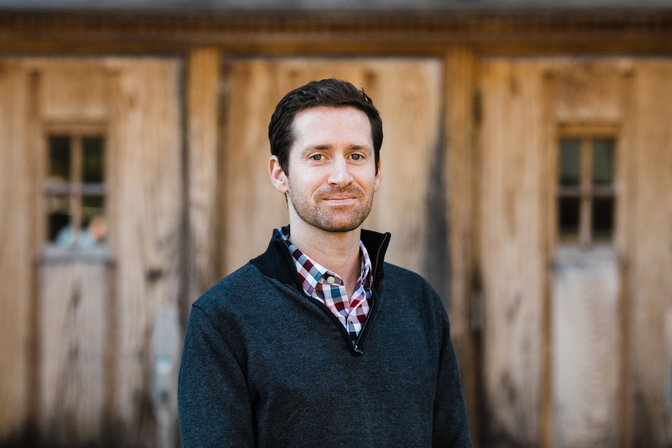
\includegraphics[width=2cm, height=2cm,
          trim={26.88px 0 26.88px 0}, clip]
          {figures/people/joe_guinness.jpg}
      \end{figure}
      Joe Guinness, \\ Cornell
    \end{column}
    \begin{column}{0.28\textwidth}
      \centering
      \begin{figure}[h!]
        \centering
        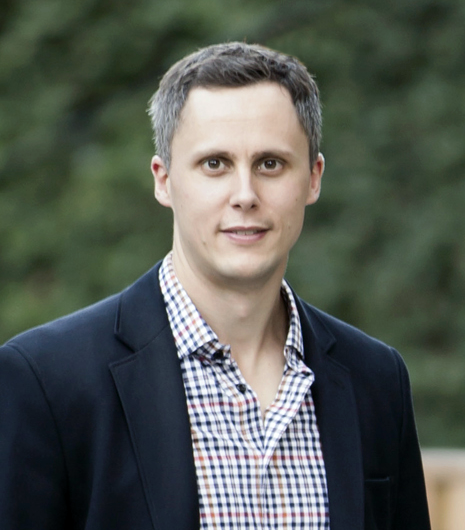
\includegraphics[width=2cm, height=2cm,
          trim={0 65px 0 0px}, clip]
          {figures/people/matthias_katzfuss.png}
      \end{figure}
      Matthias Katzfu{\ss}, \\ Texas A\&M
    \end{column}
    \begin{column}{0.26\textwidth}
      \centering
      \begin{figure}[h!]
        \centering
        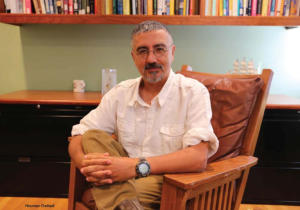
\includegraphics[width=2cm, height=2cm,
          trim={33.75px 0 33.75px 0}, clip]
          {figures/people/houman_owhadi.jpg}
      \end{figure}
      Houman Owhadi, \\ Caltech
    \end{column}
    \begin{column}{0.24\textwidth}
      \centering
      \begin{figure}[h!]
        \centering
        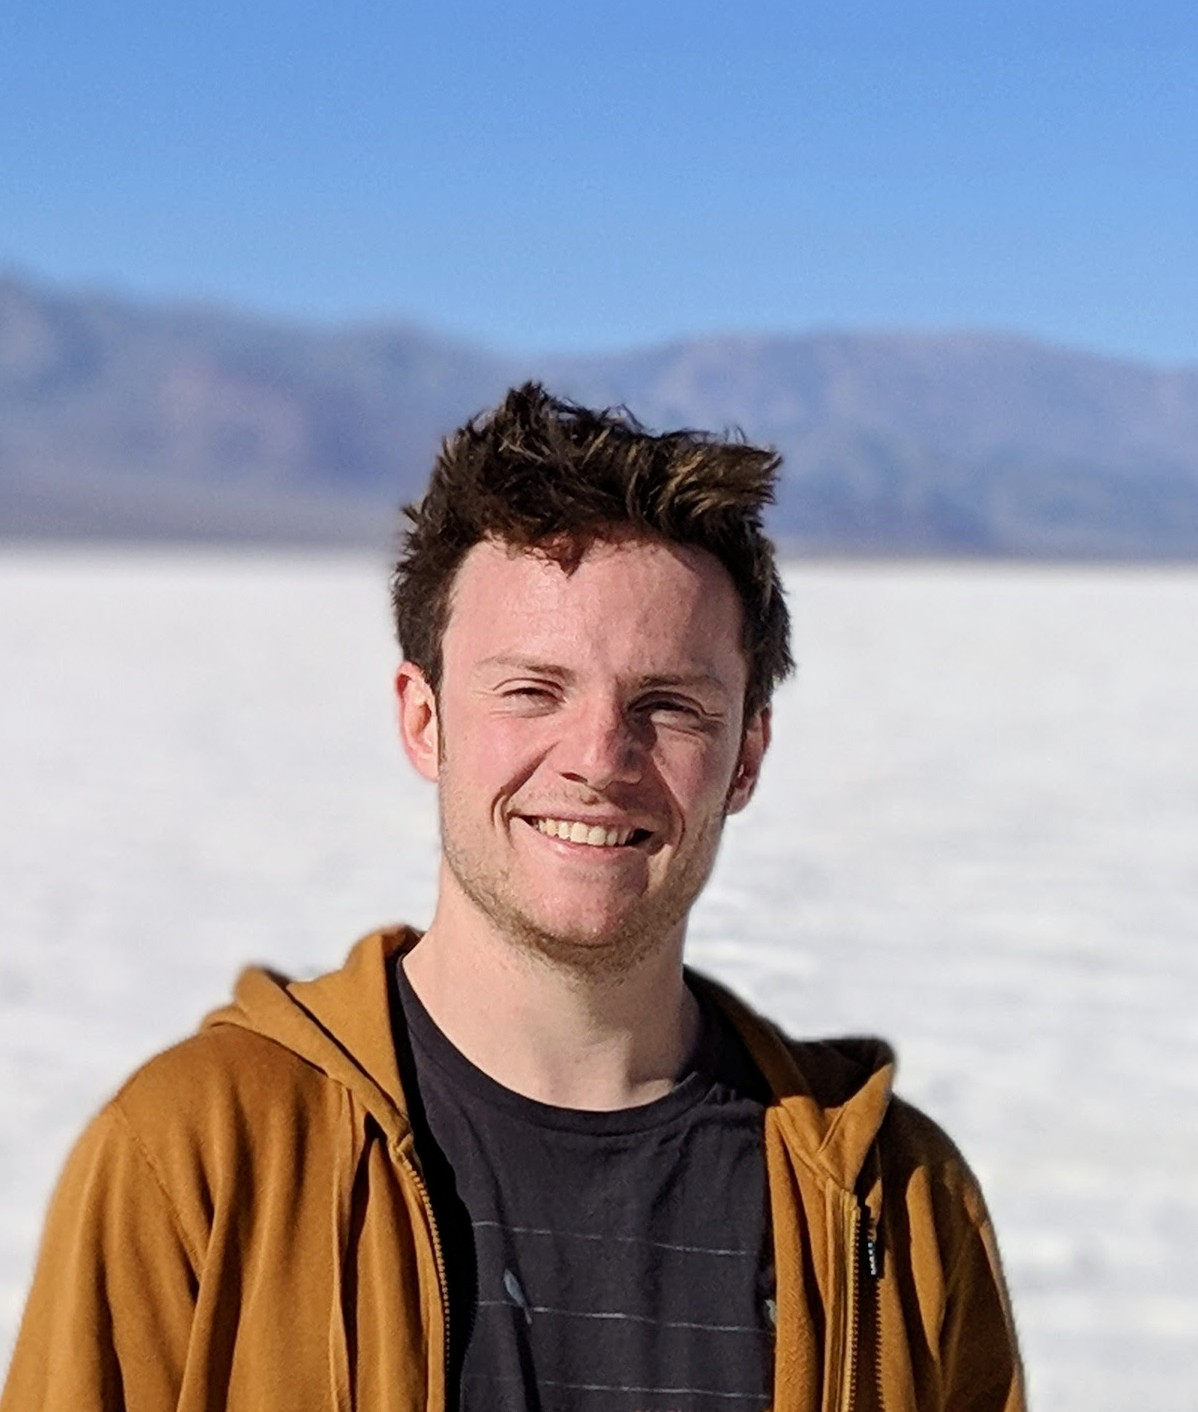
\includegraphics[width=2cm, height=2cm,
          trim={0 0 0 214px}, clip]
          {figures/people/florian_schaefer.jpg}
      \end{figure}
      Florian\ Sch{\"a}fer, Gatech
    \end{column}
  \end{columns}
\end{frame}

\begin{frame}
\frametitle{Overview}
\framesubtitle{}

\tableofcontents
\end{frame}

\begin{frame}
\frametitle{The problem}
\framesubtitle{}

\begin{wideitemize}
  \item<+-> Covariance matrices from pairwise kernel function evaluations
  \item
    i.e. \( \CM_{i, j} = \K(\vec{x}_i, \vec{x}_j) \) for points \( \{
    \vec{x}_i \}_{i = 1}^N \) and kernel function \( \K \)
  \item<+-> Kernel trick in machine learning
  \item<2-> Statistical inference in Gaussian
    processes on \( \vec{y} \sim \N(\vec{0}, \CM) \)
  \item<+-> Seek \emph{sparse} Cholesky
    factor for \emph{dense} covariance matrix
\end{wideitemize}
\end{frame}

\begin{frame}
\frametitle{Statistical Cholesky factorization}
% \framesubtitle{Covariance or precision?}

\begin{wideitemize}
  \item<+-> Factor covariance matrix \( \CM
    \) or precision matrix \( \PM = \CM^{-1} \)?
    \begin{align*}
      %    \text{marginal} & \text{ independence} &
      % \text{conditional} & \text{ independence} \\
      % \vec{y} &\sim \N(\vec{0}, \CM) &
      % \vec{y} &\sim \N(\vec{0}, \PM^{-1}) \\
      \CM_{i, i}      &= \Var[y_i] &
      \PM_{i, i}^{-1} &= \Var[y_i \mid y_{k \neq i}] \\
      % \frac{ \CM_{i, j}}{\sqrt{\CM_{i, i} \CM_{j, j}}} &= \Corr[y_i, y_j] &
      \CM_{i, j} &= \Cov[y_i, y_j] &
      % \frac{-\PM_{i, j}}{\sqrt{\PM_{i, i} \PM_{j, j}}} &=
      %   \frac{\Cov[y_i, y_j \mid y_{k \neq i, j}]}
      %        {\sqrt{\Var[y_i \mid y_{k \neq i, j}]
      %               \Var[y_j \mid y_{k \neq i, j}]}} \\
      \frac{-\PM_{i, j}}{\sqrt{\PM_{i, i} \PM_{j, j}}} &=
        \Corr[y_i, y_j \mid y_{k \neq i, j}] \\
      \intertext{
        Cholesky factorization \( \Leftrightarrow \)
        iterative conditioning of process
      }
      % observation 1 and observation 2 from phd thesis
      L &= \chol(\CM) &
      L &= \chol(\PM) \\
      L_{i, j} &=
        \frac{\Cov[y_i, y_j \mid y_{k < j}]}
       {\sqrt{\Var[y_j      \mid y_{k < j}]}} &
      -\frac{L_{i, j}}{L_{j, j}} &=
        \frac{\Cov[y_i, y_j \mid y_{k > j, k \neq i}]}
             {\Var[y_j      \mid y_{k > j, k \neq i}]}
    \end{align*}
  \item<+-> Conditional (near)-independence \(
    \Leftrightarrow \) (approximate) sparsity
  % \item<+-> Covariance matrix encodes marginal independence
  % \item<4-> Precision matrix encodes conditional independence
  \item<+-> Prefer precision matrix to attenuate density
\end{wideitemize}
\end{frame}

\begin{frame}
\frametitle{Cholesky factorization recipe}
\framesubtitle{}

\begin{wideitemize}
  \item<+-> Implied procedure for computing \( L L^{\top} \approx \CM^{-1} \)
    \begin{enumerate}
      \item Pick an ordering on the rows/columns of \( \CM \)
      \item Select a sparsity pattern lower triangular w.r.t. ordering
      \item Compute entries by minimizing objective over all factors
    \end{enumerate}
\end{wideitemize}
\end{frame}

\begin{frame}
\frametitle{Kullback-Leibler minimization}
\framesubtitle{}
\begin{wideitemize}
  \item<+-> Compute entries by minimizing Kullback-Leibler divergence
    \begin{align*}
      L \defeq \argmin_{\hat{L} \in \SpSet} \,
        \KL*{\N(\vec{0}, \CM)}
            {\N(\vec{0}, (\hat{L} \hat{L}^{\top})^{-1})}
    \end{align*}
  \item<+-> Efficient and embarrassingly parallel closed-form solution
    \begin{align*}
      L_{s_i, i} &= \frac{\CM_{s_i, s_i}^{-1} \vec{e}_1}
        {\sqrt{\vec{e}_1^{\top} \CM_{s_i, s_i}^{-1} \vec{e}_1}}
    \end{align*}
  \item<+-> Achieves state of the art \( \epsilon \)-accuracy in time
    complexity \( \BigO\left (N \log^{2d}\left (\frac{N}{\epsilon} \right
    ) \right ) \) with \( \BigO\left (N \log^{d}\left (\frac{N}{\epsilon}
    \right ) \right ) \) nonzero entries [\cite{schafer2021sparse}]
\end{wideitemize}
\end{frame}

\begin{frame}
\frametitle{Screening effect}
\framesubtitle{}

\begin{figure}[t]
  \centering
  \begin{tikzpicture}[baseline]
  \begin{axis}[
    width={0.49\linewidth},
    grid={major},
    % axis lines=none,
    ticks=none,
    xmin=-1.1, xmax=1.1, ymin=-1.1, ymax=1.1, zmin=-0.1, zmax=1,
  ]
  \addplot3 [only marks, orange]
    table {figures/screening/matern_uncond_points.csv};
  \addplot3 [mesh, lightblue]
    table {figures/screening/matern_uncond.csv};
  \end{axis}
\end{tikzpicture}
%
  \qquad
  \begin{tikzpicture}[baseline]
  \begin{axis}[
    width={0.49\linewidth},
    grid={major},
    % axis lines=none,
    ticks=none,
    xmin=-1.1, xmax=1.1, ymin=-1.1, ymax=1.1, zmin=-0.1, zmax=1,
  ]
  \addplot3 [only marks, orange]
    table {figures/screening/matern_cond_points.csv};
  \addplot3 [mesh, seagreen]
    table {figures/screening/matern_cond.csv};
  \end{axis}
\end{tikzpicture}

  \label{fig:screening}
\end{figure}

\begin{wideitemize}
  \item<+-> Conditional on points near a point of interest, \\
    far away points are almost independent [\cite{stein2002screening}]
  \item<+-> Suggests space-covering ordering
    and selecting nearby points % for the sparsity
\end{wideitemize}
\end{frame}

\section{Previous work}

\begin{frame}
\frametitle{Ordering and sparsity pattern}
\framesubtitle{}

% copied a bit from https://youtu.be/Hdhv-moeR5U?t=968
\begin{wideitemize}
  \item (Reverse) maximin ordering [\cite{guinness2018permutation}]
    selects the next \textcolor{orange}{point \( \vec{x}_i \)}
    with \textcolor{orange}{largest distance \( \ell_i \)} to
    \textcolor{lightblue}{points selected before}
  \item The \( i \)th column selects all points
    within a radius of \textcolor{seagreen}{\( \rho
    \ell_i \)} from \textcolor{orange}{\( \vec{x}_i \)}
\end{wideitemize}

% computer generated
\only<1>{
  \begin{figure}
    \centering
    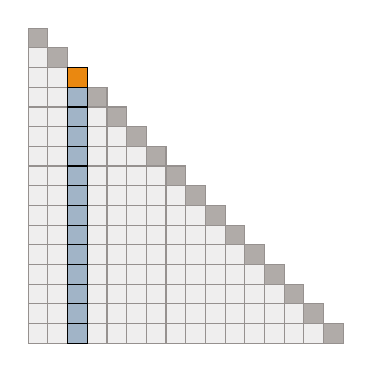
\begin{tikzpicture}[scale=4/16]
  \filldraw[draw=nnzborder, fill=nnzcolor] (0, 0) rectangle (1, -1);
  \filldraw[draw=zeroborder, fill=zerocolor] (0, -1) rectangle (1, -2);
  \filldraw[draw=zeroborder, fill=zerocolor] (0, -2) rectangle (1, -3);
  \filldraw[draw=zeroborder, fill=zerocolor] (0, -3) rectangle (1, -4);
  \filldraw[draw=zeroborder, fill=zerocolor] (0, -4) rectangle (1, -5);
  \filldraw[draw=zeroborder, fill=zerocolor] (0, -5) rectangle (1, -6);
  \filldraw[draw=zeroborder, fill=zerocolor] (0, -6) rectangle (1, -7);
  \filldraw[draw=zeroborder, fill=zerocolor] (0, -7) rectangle (1, -8);
  \filldraw[draw=zeroborder, fill=zerocolor] (0, -8) rectangle (1, -9);
  \filldraw[draw=zeroborder, fill=zerocolor] (0, -9) rectangle (1, -10);
  \filldraw[draw=zeroborder, fill=zerocolor] (0, -10) rectangle (1, -11);
  \filldraw[draw=zeroborder, fill=zerocolor] (0, -11) rectangle (1, -12);
  \filldraw[draw=zeroborder, fill=zerocolor] (0, -12) rectangle (1, -13);
  \filldraw[draw=zeroborder, fill=zerocolor] (0, -13) rectangle (1, -14);
  \filldraw[draw=zeroborder, fill=zerocolor] (0, -14) rectangle (1, -15);
  \filldraw[draw=zeroborder, fill=zerocolor] (0, -15) rectangle (1, -16);
  \filldraw[draw=nnzborder, fill=nnzcolor] (1, -1) rectangle (2, -2);
  \filldraw[draw=zeroborder, fill=zerocolor] (1, -2) rectangle (2, -3);
  \filldraw[draw=zeroborder, fill=zerocolor] (1, -3) rectangle (2, -4);
  \filldraw[draw=zeroborder, fill=zerocolor] (1, -4) rectangle (2, -5);
  \filldraw[draw=zeroborder, fill=zerocolor] (1, -5) rectangle (2, -6);
  \filldraw[draw=zeroborder, fill=zerocolor] (1, -6) rectangle (2, -7);
  \filldraw[draw=zeroborder, fill=zerocolor] (1, -7) rectangle (2, -8);
  \filldraw[draw=zeroborder, fill=zerocolor] (1, -8) rectangle (2, -9);
  \filldraw[draw=zeroborder, fill=zerocolor] (1, -9) rectangle (2, -10);
  \filldraw[draw=zeroborder, fill=zerocolor] (1, -10) rectangle (2, -11);
  \filldraw[draw=zeroborder, fill=zerocolor] (1, -11) rectangle (2, -12);
  \filldraw[draw=zeroborder, fill=zerocolor] (1, -12) rectangle (2, -13);
  \filldraw[draw=zeroborder, fill=zerocolor] (1, -13) rectangle (2, -14);
  \filldraw[draw=zeroborder, fill=zerocolor] (1, -14) rectangle (2, -15);
  \filldraw[draw=zeroborder, fill=zerocolor] (1, -15) rectangle (2, -16);
  \filldraw[draw=nnzborder, fill=nnzcolor] (3, -3) rectangle (4, -4);
  \filldraw[draw=zeroborder, fill=zerocolor] (3, -4) rectangle (4, -5);
  \filldraw[draw=zeroborder, fill=zerocolor] (3, -5) rectangle (4, -6);
  \filldraw[draw=zeroborder, fill=zerocolor] (3, -6) rectangle (4, -7);
  \filldraw[draw=zeroborder, fill=zerocolor] (3, -7) rectangle (4, -8);
  \filldraw[draw=zeroborder, fill=zerocolor] (3, -8) rectangle (4, -9);
  \filldraw[draw=zeroborder, fill=zerocolor] (3, -9) rectangle (4, -10);
  \filldraw[draw=zeroborder, fill=zerocolor] (3, -10) rectangle (4, -11);
  \filldraw[draw=zeroborder, fill=zerocolor] (3, -11) rectangle (4, -12);
  \filldraw[draw=zeroborder, fill=zerocolor] (3, -12) rectangle (4, -13);
  \filldraw[draw=zeroborder, fill=zerocolor] (3, -13) rectangle (4, -14);
  \filldraw[draw=zeroborder, fill=zerocolor] (3, -14) rectangle (4, -15);
  \filldraw[draw=zeroborder, fill=zerocolor] (3, -15) rectangle (4, -16);
  \filldraw[draw=nnzborder, fill=nnzcolor] (4, -4) rectangle (5, -5);
  \filldraw[draw=zeroborder, fill=zerocolor] (4, -5) rectangle (5, -6);
  \filldraw[draw=zeroborder, fill=zerocolor] (4, -6) rectangle (5, -7);
  \filldraw[draw=zeroborder, fill=zerocolor] (4, -7) rectangle (5, -8);
  \filldraw[draw=zeroborder, fill=zerocolor] (4, -8) rectangle (5, -9);
  \filldraw[draw=zeroborder, fill=zerocolor] (4, -9) rectangle (5, -10);
  \filldraw[draw=zeroborder, fill=zerocolor] (4, -10) rectangle (5, -11);
  \filldraw[draw=zeroborder, fill=zerocolor] (4, -11) rectangle (5, -12);
  \filldraw[draw=zeroborder, fill=zerocolor] (4, -12) rectangle (5, -13);
  \filldraw[draw=zeroborder, fill=zerocolor] (4, -13) rectangle (5, -14);
  \filldraw[draw=zeroborder, fill=zerocolor] (4, -14) rectangle (5, -15);
  \filldraw[draw=zeroborder, fill=zerocolor] (4, -15) rectangle (5, -16);
  \filldraw[draw=nnzborder, fill=nnzcolor] (5, -5) rectangle (6, -6);
  \filldraw[draw=zeroborder, fill=zerocolor] (5, -6) rectangle (6, -7);
  \filldraw[draw=zeroborder, fill=zerocolor] (5, -7) rectangle (6, -8);
  \filldraw[draw=zeroborder, fill=zerocolor] (5, -8) rectangle (6, -9);
  \filldraw[draw=zeroborder, fill=zerocolor] (5, -9) rectangle (6, -10);
  \filldraw[draw=zeroborder, fill=zerocolor] (5, -10) rectangle (6, -11);
  \filldraw[draw=zeroborder, fill=zerocolor] (5, -11) rectangle (6, -12);
  \filldraw[draw=zeroborder, fill=zerocolor] (5, -12) rectangle (6, -13);
  \filldraw[draw=zeroborder, fill=zerocolor] (5, -13) rectangle (6, -14);
  \filldraw[draw=zeroborder, fill=zerocolor] (5, -14) rectangle (6, -15);
  \filldraw[draw=zeroborder, fill=zerocolor] (5, -15) rectangle (6, -16);
  \filldraw[draw=nnzborder, fill=nnzcolor] (6, -6) rectangle (7, -7);
  \filldraw[draw=zeroborder, fill=zerocolor] (6, -7) rectangle (7, -8);
  \filldraw[draw=zeroborder, fill=zerocolor] (6, -8) rectangle (7, -9);
  \filldraw[draw=zeroborder, fill=zerocolor] (6, -9) rectangle (7, -10);
  \filldraw[draw=zeroborder, fill=zerocolor] (6, -10) rectangle (7, -11);
  \filldraw[draw=zeroborder, fill=zerocolor] (6, -11) rectangle (7, -12);
  \filldraw[draw=zeroborder, fill=zerocolor] (6, -12) rectangle (7, -13);
  \filldraw[draw=zeroborder, fill=zerocolor] (6, -13) rectangle (7, -14);
  \filldraw[draw=zeroborder, fill=zerocolor] (6, -14) rectangle (7, -15);
  \filldraw[draw=zeroborder, fill=zerocolor] (6, -15) rectangle (7, -16);
  \filldraw[draw=nnzborder, fill=nnzcolor] (7, -7) rectangle (8, -8);
  \filldraw[draw=zeroborder, fill=zerocolor] (7, -8) rectangle (8, -9);
  \filldraw[draw=zeroborder, fill=zerocolor] (7, -9) rectangle (8, -10);
  \filldraw[draw=zeroborder, fill=zerocolor] (7, -10) rectangle (8, -11);
  \filldraw[draw=zeroborder, fill=zerocolor] (7, -11) rectangle (8, -12);
  \filldraw[draw=zeroborder, fill=zerocolor] (7, -12) rectangle (8, -13);
  \filldraw[draw=zeroborder, fill=zerocolor] (7, -13) rectangle (8, -14);
  \filldraw[draw=zeroborder, fill=zerocolor] (7, -14) rectangle (8, -15);
  \filldraw[draw=zeroborder, fill=zerocolor] (7, -15) rectangle (8, -16);
  \filldraw[draw=nnzborder, fill=nnzcolor] (8, -8) rectangle (9, -9);
  \filldraw[draw=zeroborder, fill=zerocolor] (8, -9) rectangle (9, -10);
  \filldraw[draw=zeroborder, fill=zerocolor] (8, -10) rectangle (9, -11);
  \filldraw[draw=zeroborder, fill=zerocolor] (8, -11) rectangle (9, -12);
  \filldraw[draw=zeroborder, fill=zerocolor] (8, -12) rectangle (9, -13);
  \filldraw[draw=zeroborder, fill=zerocolor] (8, -13) rectangle (9, -14);
  \filldraw[draw=zeroborder, fill=zerocolor] (8, -14) rectangle (9, -15);
  \filldraw[draw=zeroborder, fill=zerocolor] (8, -15) rectangle (9, -16);
  \filldraw[draw=nnzborder, fill=nnzcolor] (9, -9) rectangle (10, -10);
  \filldraw[draw=zeroborder, fill=zerocolor] (9, -10) rectangle (10, -11);
  \filldraw[draw=zeroborder, fill=zerocolor] (9, -11) rectangle (10, -12);
  \filldraw[draw=zeroborder, fill=zerocolor] (9, -12) rectangle (10, -13);
  \filldraw[draw=zeroborder, fill=zerocolor] (9, -13) rectangle (10, -14);
  \filldraw[draw=zeroborder, fill=zerocolor] (9, -14) rectangle (10, -15);
  \filldraw[draw=zeroborder, fill=zerocolor] (9, -15) rectangle (10, -16);
  \filldraw[draw=nnzborder, fill=nnzcolor] (10, -10) rectangle (11, -11);
  \filldraw[draw=zeroborder, fill=zerocolor] (10, -11) rectangle (11, -12);
  \filldraw[draw=zeroborder, fill=zerocolor] (10, -12) rectangle (11, -13);
  \filldraw[draw=zeroborder, fill=zerocolor] (10, -13) rectangle (11, -14);
  \filldraw[draw=zeroborder, fill=zerocolor] (10, -14) rectangle (11, -15);
  \filldraw[draw=zeroborder, fill=zerocolor] (10, -15) rectangle (11, -16);
  \filldraw[draw=nnzborder, fill=nnzcolor] (11, -11) rectangle (12, -12);
  \filldraw[draw=zeroborder, fill=zerocolor] (11, -12) rectangle (12, -13);
  \filldraw[draw=zeroborder, fill=zerocolor] (11, -13) rectangle (12, -14);
  \filldraw[draw=zeroborder, fill=zerocolor] (11, -14) rectangle (12, -15);
  \filldraw[draw=zeroborder, fill=zerocolor] (11, -15) rectangle (12, -16);
  \filldraw[draw=nnzborder, fill=nnzcolor] (12, -12) rectangle (13, -13);
  \filldraw[draw=zeroborder, fill=zerocolor] (12, -13) rectangle (13, -14);
  \filldraw[draw=zeroborder, fill=zerocolor] (12, -14) rectangle (13, -15);
  \filldraw[draw=zeroborder, fill=zerocolor] (12, -15) rectangle (13, -16);
  \filldraw[draw=nnzborder, fill=nnzcolor] (13, -13) rectangle (14, -14);
  \filldraw[draw=zeroborder, fill=zerocolor] (13, -14) rectangle (14, -15);
  \filldraw[draw=zeroborder, fill=zerocolor] (13, -15) rectangle (14, -16);
  \filldraw[draw=nnzborder, fill=nnzcolor] (14, -14) rectangle (15, -15);
  \filldraw[draw=zeroborder, fill=zerocolor] (14, -15) rectangle (15, -16);
  \filldraw[draw=nnzborder, fill=nnzcolor] (15, -15) rectangle (16, -16);
  \filldraw[draw=colborder, fill=targetcolor] (2, -2) rectangle (3, -3);
  \filldraw[draw=colborder, fill=candcolor] (2, -3) rectangle (3, -4);
  \filldraw[draw=colborder, fill=candcolor] (2, -4) rectangle (3, -5);
  \filldraw[draw=colborder, fill=candcolor] (2, -5) rectangle (3, -6);
  \filldraw[draw=colborder, fill=candcolor] (2, -6) rectangle (3, -7);
  \filldraw[draw=colborder, fill=candcolor] (2, -7) rectangle (3, -8);
  \filldraw[draw=colborder, fill=candcolor] (2, -8) rectangle (3, -9);
  \filldraw[draw=colborder, fill=candcolor] (2, -9) rectangle (3, -10);
  \filldraw[draw=colborder, fill=candcolor] (2, -10) rectangle (3, -11);
  \filldraw[draw=colborder, fill=candcolor] (2, -11) rectangle (3, -12);
  \filldraw[draw=colborder, fill=candcolor] (2, -12) rectangle (3, -13);
  \filldraw[draw=colborder, fill=candcolor] (2, -13) rectangle (3, -14);
  \filldraw[draw=colborder, fill=candcolor] (2, -14) rectangle (3, -15);
  \filldraw[draw=colborder, fill=candcolor] (2, -15) rectangle (3, -16);
\end{tikzpicture}
%
    \qquad
    \begin{tikzpicture}[baseline]
  \begin{axis}[
    % calculated from Cholesky factor, exactly 16 cm x 16 cm
    width={4cm},
    height={4cm},
    axis lines={none},
    % force axis box to have exactly the right dimensions, ignoring labels
    scale only axis=true,
  ]
  % consistent size bounding box
  \draw [white, line width=0] (-0.1, -0.1) -- (-0.1,  1.1);
  \draw [white, line width=0] ( 1.1, -0.1) -- ( 1.1,  1.1);
  \draw [white, line width=0] (-0.1, -0.1) -- (-1.1, -0.1);
  \draw [white, line width=0] (-0.1,  1.1) -- (-1.1,  1.1);
  \draw [seagreen!15, fill, radius=4.0] (0.08564916714362436, 0.2368105065960997) circle;
  \draw [seagreen, radius=4.0] (0.08564916714362436, 0.2368105065960997) circle;
  \draw [orange!25, fill, radius=2.0] (0.08564916714362436, 0.2368105065960997) circle;
  \draw [orange, radius=2.0] (0.08564916714362436, 0.2368105065960997) circle;
  \addplot [only marks, mark size=1, silver]    table
    {figures/points_knn/all_points.csv};
  \addplot [only marks, mark size=2, lightblue] table
    {figures/points_knn/candidates_01.csv};
  \addplot [only marks, mark size=4, seagreen]  table
    {figures/points_knn/selected_01.csv};
  \addplot [only marks, mark size=4, orange]    table
    {figures/points_knn/target_01.csv};
  \end{axis}
\end{tikzpicture}

  \end{figure}
}
\only<2>{
  \begin{figure}
    \centering
    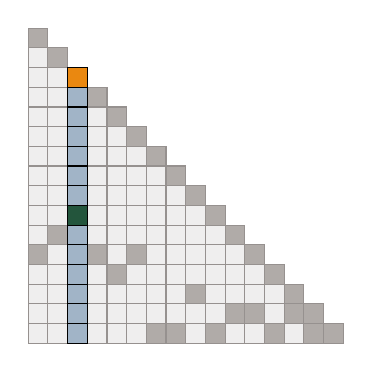
\begin{tikzpicture}[scale=4/16]
  \filldraw[draw=nnzborder, fill=nnzcolor] (0, 0) rectangle (1, -1);
  \filldraw[draw=zeroborder, fill=zerocolor] (0, -1) rectangle (1, -2);
  \filldraw[draw=zeroborder, fill=zerocolor] (0, -2) rectangle (1, -3);
  \filldraw[draw=zeroborder, fill=zerocolor] (0, -3) rectangle (1, -4);
  \filldraw[draw=zeroborder, fill=zerocolor] (0, -4) rectangle (1, -5);
  \filldraw[draw=zeroborder, fill=zerocolor] (0, -5) rectangle (1, -6);
  \filldraw[draw=zeroborder, fill=zerocolor] (0, -6) rectangle (1, -7);
  \filldraw[draw=zeroborder, fill=zerocolor] (0, -7) rectangle (1, -8);
  \filldraw[draw=zeroborder, fill=zerocolor] (0, -8) rectangle (1, -9);
  \filldraw[draw=zeroborder, fill=zerocolor] (0, -9) rectangle (1, -10);
  \filldraw[draw=zeroborder, fill=zerocolor] (0, -10) rectangle (1, -11);
  \filldraw[draw=nnzborder, fill=nnzcolor] (0, -11) rectangle (1, -12);
  \filldraw[draw=zeroborder, fill=zerocolor] (0, -12) rectangle (1, -13);
  \filldraw[draw=zeroborder, fill=zerocolor] (0, -13) rectangle (1, -14);
  \filldraw[draw=zeroborder, fill=zerocolor] (0, -14) rectangle (1, -15);
  \filldraw[draw=zeroborder, fill=zerocolor] (0, -15) rectangle (1, -16);
  \filldraw[draw=nnzborder, fill=nnzcolor] (1, -1) rectangle (2, -2);
  \filldraw[draw=zeroborder, fill=zerocolor] (1, -2) rectangle (2, -3);
  \filldraw[draw=zeroborder, fill=zerocolor] (1, -3) rectangle (2, -4);
  \filldraw[draw=zeroborder, fill=zerocolor] (1, -4) rectangle (2, -5);
  \filldraw[draw=zeroborder, fill=zerocolor] (1, -5) rectangle (2, -6);
  \filldraw[draw=zeroborder, fill=zerocolor] (1, -6) rectangle (2, -7);
  \filldraw[draw=zeroborder, fill=zerocolor] (1, -7) rectangle (2, -8);
  \filldraw[draw=zeroborder, fill=zerocolor] (1, -8) rectangle (2, -9);
  \filldraw[draw=zeroborder, fill=zerocolor] (1, -9) rectangle (2, -10);
  \filldraw[draw=nnzborder, fill=nnzcolor] (1, -10) rectangle (2, -11);
  \filldraw[draw=zeroborder, fill=zerocolor] (1, -11) rectangle (2, -12);
  \filldraw[draw=zeroborder, fill=zerocolor] (1, -12) rectangle (2, -13);
  \filldraw[draw=zeroborder, fill=zerocolor] (1, -13) rectangle (2, -14);
  \filldraw[draw=zeroborder, fill=zerocolor] (1, -14) rectangle (2, -15);
  \filldraw[draw=zeroborder, fill=zerocolor] (1, -15) rectangle (2, -16);
  \filldraw[draw=nnzborder, fill=nnzcolor] (3, -3) rectangle (4, -4);
  \filldraw[draw=zeroborder, fill=zerocolor] (3, -4) rectangle (4, -5);
  \filldraw[draw=zeroborder, fill=zerocolor] (3, -5) rectangle (4, -6);
  \filldraw[draw=zeroborder, fill=zerocolor] (3, -6) rectangle (4, -7);
  \filldraw[draw=zeroborder, fill=zerocolor] (3, -7) rectangle (4, -8);
  \filldraw[draw=zeroborder, fill=zerocolor] (3, -8) rectangle (4, -9);
  \filldraw[draw=zeroborder, fill=zerocolor] (3, -9) rectangle (4, -10);
  \filldraw[draw=zeroborder, fill=zerocolor] (3, -10) rectangle (4, -11);
  \filldraw[draw=nnzborder, fill=nnzcolor] (3, -11) rectangle (4, -12);
  \filldraw[draw=zeroborder, fill=zerocolor] (3, -12) rectangle (4, -13);
  \filldraw[draw=zeroborder, fill=zerocolor] (3, -13) rectangle (4, -14);
  \filldraw[draw=zeroborder, fill=zerocolor] (3, -14) rectangle (4, -15);
  \filldraw[draw=zeroborder, fill=zerocolor] (3, -15) rectangle (4, -16);
  \filldraw[draw=nnzborder, fill=nnzcolor] (4, -4) rectangle (5, -5);
  \filldraw[draw=zeroborder, fill=zerocolor] (4, -5) rectangle (5, -6);
  \filldraw[draw=zeroborder, fill=zerocolor] (4, -6) rectangle (5, -7);
  \filldraw[draw=zeroborder, fill=zerocolor] (4, -7) rectangle (5, -8);
  \filldraw[draw=zeroborder, fill=zerocolor] (4, -8) rectangle (5, -9);
  \filldraw[draw=zeroborder, fill=zerocolor] (4, -9) rectangle (5, -10);
  \filldraw[draw=zeroborder, fill=zerocolor] (4, -10) rectangle (5, -11);
  \filldraw[draw=zeroborder, fill=zerocolor] (4, -11) rectangle (5, -12);
  \filldraw[draw=nnzborder, fill=nnzcolor] (4, -12) rectangle (5, -13);
  \filldraw[draw=zeroborder, fill=zerocolor] (4, -13) rectangle (5, -14);
  \filldraw[draw=zeroborder, fill=zerocolor] (4, -14) rectangle (5, -15);
  \filldraw[draw=zeroborder, fill=zerocolor] (4, -15) rectangle (5, -16);
  \filldraw[draw=nnzborder, fill=nnzcolor] (5, -5) rectangle (6, -6);
  \filldraw[draw=zeroborder, fill=zerocolor] (5, -6) rectangle (6, -7);
  \filldraw[draw=zeroborder, fill=zerocolor] (5, -7) rectangle (6, -8);
  \filldraw[draw=zeroborder, fill=zerocolor] (5, -8) rectangle (6, -9);
  \filldraw[draw=zeroborder, fill=zerocolor] (5, -9) rectangle (6, -10);
  \filldraw[draw=zeroborder, fill=zerocolor] (5, -10) rectangle (6, -11);
  \filldraw[draw=nnzborder, fill=nnzcolor] (5, -11) rectangle (6, -12);
  \filldraw[draw=zeroborder, fill=zerocolor] (5, -12) rectangle (6, -13);
  \filldraw[draw=zeroborder, fill=zerocolor] (5, -13) rectangle (6, -14);
  \filldraw[draw=zeroborder, fill=zerocolor] (5, -14) rectangle (6, -15);
  \filldraw[draw=zeroborder, fill=zerocolor] (5, -15) rectangle (6, -16);
  \filldraw[draw=nnzborder, fill=nnzcolor] (6, -6) rectangle (7, -7);
  \filldraw[draw=zeroborder, fill=zerocolor] (6, -7) rectangle (7, -8);
  \filldraw[draw=zeroborder, fill=zerocolor] (6, -8) rectangle (7, -9);
  \filldraw[draw=zeroborder, fill=zerocolor] (6, -9) rectangle (7, -10);
  \filldraw[draw=zeroborder, fill=zerocolor] (6, -10) rectangle (7, -11);
  \filldraw[draw=zeroborder, fill=zerocolor] (6, -11) rectangle (7, -12);
  \filldraw[draw=zeroborder, fill=zerocolor] (6, -12) rectangle (7, -13);
  \filldraw[draw=zeroborder, fill=zerocolor] (6, -13) rectangle (7, -14);
  \filldraw[draw=zeroborder, fill=zerocolor] (6, -14) rectangle (7, -15);
  \filldraw[draw=nnzborder, fill=nnzcolor] (6, -15) rectangle (7, -16);
  \filldraw[draw=nnzborder, fill=nnzcolor] (7, -7) rectangle (8, -8);
  \filldraw[draw=zeroborder, fill=zerocolor] (7, -8) rectangle (8, -9);
  \filldraw[draw=zeroborder, fill=zerocolor] (7, -9) rectangle (8, -10);
  \filldraw[draw=zeroborder, fill=zerocolor] (7, -10) rectangle (8, -11);
  \filldraw[draw=zeroborder, fill=zerocolor] (7, -11) rectangle (8, -12);
  \filldraw[draw=zeroborder, fill=zerocolor] (7, -12) rectangle (8, -13);
  \filldraw[draw=zeroborder, fill=zerocolor] (7, -13) rectangle (8, -14);
  \filldraw[draw=zeroborder, fill=zerocolor] (7, -14) rectangle (8, -15);
  \filldraw[draw=nnzborder, fill=nnzcolor] (7, -15) rectangle (8, -16);
  \filldraw[draw=nnzborder, fill=nnzcolor] (8, -8) rectangle (9, -9);
  \filldraw[draw=zeroborder, fill=zerocolor] (8, -9) rectangle (9, -10);
  \filldraw[draw=zeroborder, fill=zerocolor] (8, -10) rectangle (9, -11);
  \filldraw[draw=zeroborder, fill=zerocolor] (8, -11) rectangle (9, -12);
  \filldraw[draw=zeroborder, fill=zerocolor] (8, -12) rectangle (9, -13);
  \filldraw[draw=nnzborder, fill=nnzcolor] (8, -13) rectangle (9, -14);
  \filldraw[draw=zeroborder, fill=zerocolor] (8, -14) rectangle (9, -15);
  \filldraw[draw=zeroborder, fill=zerocolor] (8, -15) rectangle (9, -16);
  \filldraw[draw=nnzborder, fill=nnzcolor] (9, -9) rectangle (10, -10);
  \filldraw[draw=zeroborder, fill=zerocolor] (9, -10) rectangle (10, -11);
  \filldraw[draw=zeroborder, fill=zerocolor] (9, -11) rectangle (10, -12);
  \filldraw[draw=zeroborder, fill=zerocolor] (9, -12) rectangle (10, -13);
  \filldraw[draw=zeroborder, fill=zerocolor] (9, -13) rectangle (10, -14);
  \filldraw[draw=zeroborder, fill=zerocolor] (9, -14) rectangle (10, -15);
  \filldraw[draw=nnzborder, fill=nnzcolor] (9, -15) rectangle (10, -16);
  \filldraw[draw=nnzborder, fill=nnzcolor] (10, -10) rectangle (11, -11);
  \filldraw[draw=zeroborder, fill=zerocolor] (10, -11) rectangle (11, -12);
  \filldraw[draw=zeroborder, fill=zerocolor] (10, -12) rectangle (11, -13);
  \filldraw[draw=zeroborder, fill=zerocolor] (10, -13) rectangle (11, -14);
  \filldraw[draw=nnzborder, fill=nnzcolor] (10, -14) rectangle (11, -15);
  \filldraw[draw=zeroborder, fill=zerocolor] (10, -15) rectangle (11, -16);
  \filldraw[draw=nnzborder, fill=nnzcolor] (11, -11) rectangle (12, -12);
  \filldraw[draw=zeroborder, fill=zerocolor] (11, -12) rectangle (12, -13);
  \filldraw[draw=zeroborder, fill=zerocolor] (11, -13) rectangle (12, -14);
  \filldraw[draw=nnzborder, fill=nnzcolor] (11, -14) rectangle (12, -15);
  \filldraw[draw=zeroborder, fill=zerocolor] (11, -15) rectangle (12, -16);
  \filldraw[draw=nnzborder, fill=nnzcolor] (12, -12) rectangle (13, -13);
  \filldraw[draw=zeroborder, fill=zerocolor] (12, -13) rectangle (13, -14);
  \filldraw[draw=zeroborder, fill=zerocolor] (12, -14) rectangle (13, -15);
  \filldraw[draw=nnzborder, fill=nnzcolor] (12, -15) rectangle (13, -16);
  \filldraw[draw=nnzborder, fill=nnzcolor] (13, -13) rectangle (14, -14);
  \filldraw[draw=nnzborder, fill=nnzcolor] (13, -14) rectangle (14, -15);
  \filldraw[draw=zeroborder, fill=zerocolor] (13, -15) rectangle (14, -16);
  \filldraw[draw=nnzborder, fill=nnzcolor] (14, -14) rectangle (15, -15);
  \filldraw[draw=nnzborder, fill=nnzcolor] (14, -15) rectangle (15, -16);
  \filldraw[draw=nnzborder, fill=nnzcolor] (15, -15) rectangle (16, -16);
  \filldraw[draw=colborder, fill=targetcolor] (2, -2) rectangle (3, -3);
  \filldraw[draw=colborder, fill=candcolor] (2, -3) rectangle (3, -4);
  \filldraw[draw=colborder, fill=candcolor] (2, -4) rectangle (3, -5);
  \filldraw[draw=colborder, fill=candcolor] (2, -5) rectangle (3, -6);
  \filldraw[draw=colborder, fill=candcolor] (2, -6) rectangle (3, -7);
  \filldraw[draw=colborder, fill=candcolor] (2, -7) rectangle (3, -8);
  \filldraw[draw=colborder, fill=candcolor] (2, -8) rectangle (3, -9);
  \filldraw[draw=colborder, fill=selcolor] (2, -9) rectangle (3, -10);
  \filldraw[draw=colborder, fill=candcolor] (2, -10) rectangle (3, -11);
  \filldraw[draw=colborder, fill=candcolor] (2, -11) rectangle (3, -12);
  \filldraw[draw=colborder, fill=candcolor] (2, -12) rectangle (3, -13);
  \filldraw[draw=colborder, fill=candcolor] (2, -13) rectangle (3, -14);
  \filldraw[draw=colborder, fill=candcolor] (2, -14) rectangle (3, -15);
  \filldraw[draw=colborder, fill=candcolor] (2, -15) rectangle (3, -16);
\end{tikzpicture}
%
    \qquad
    \begin{tikzpicture}[baseline]
  \begin{axis}[
    % calculated from Cholesky factor, exactly 16 cm x 16 cm
    width={4cm},
    height={4cm},
    axis lines={none},
    % force axis box to have exactly the right dimensions, ignoring labels
    scale only axis=true,
  ]
  % consistent size bounding box
  \draw [white, line width=0] (-0.1, -0.1) -- (-0.1,  1.1);
  \draw [white, line width=0] ( 1.1, -0.1) -- ( 1.1,  1.1);
  \draw [white, line width=0] (-0.1, -0.1) -- (-1.1, -0.1);
  \draw [white, line width=0] (-0.1,  1.1) -- (-1.1,  1.1);
  \draw [seagreen!15, fill, radius=1.9421300888061523] (0.7378377872921602, 0.9562672548360985) circle;
  \draw [seagreen, radius=1.9421300888061523] (0.7378377872921602, 0.9562672548360985) circle;
  \draw [orange!25, fill, radius=0.9710650444030762] (0.7378377872921602, 0.9562672548360985) circle;
  \draw [orange, radius=0.9710650444030762] (0.7378377872921602, 0.9562672548360985) circle;
  \addplot [only marks, mark size=1, silver]    table
    {figures/points_knn/all_points.csv};
  \addplot [only marks, mark size=2, lightblue] table
    {figures/points_knn/candidates_02.csv};
  \addplot [only marks, mark size=4, seagreen]  table
    {figures/points_knn/selected_02.csv};
  \addplot [only marks, mark size=4, orange]    table
    {figures/points_knn/target_02.csv};
  \end{axis}
\end{tikzpicture}

  \end{figure}
}
\only<3>{
  \begin{figure}
    \centering
    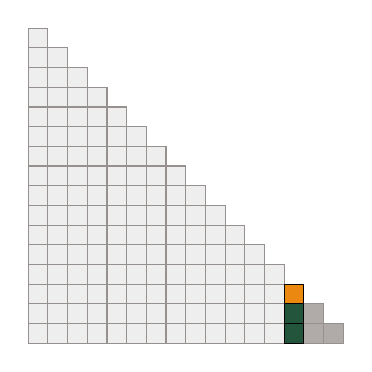
\begin{tikzpicture}[scale=4/16]
  \filldraw[draw=zeroborder, fill=zerocolor] (0, 0) rectangle (1, -1);
  \filldraw[draw=zeroborder, fill=zerocolor] (0, -1) rectangle (1, -2);
  \filldraw[draw=zeroborder, fill=zerocolor] (0, -2) rectangle (1, -3);
  \filldraw[draw=zeroborder, fill=zerocolor] (0, -3) rectangle (1, -4);
  \filldraw[draw=zeroborder, fill=zerocolor] (0, -4) rectangle (1, -5);
  \filldraw[draw=zeroborder, fill=zerocolor] (0, -5) rectangle (1, -6);
  \filldraw[draw=zeroborder, fill=zerocolor] (0, -6) rectangle (1, -7);
  \filldraw[draw=zeroborder, fill=zerocolor] (0, -7) rectangle (1, -8);
  \filldraw[draw=zeroborder, fill=zerocolor] (0, -8) rectangle (1, -9);
  \filldraw[draw=zeroborder, fill=zerocolor] (0, -9) rectangle (1, -10);
  \filldraw[draw=zeroborder, fill=zerocolor] (0, -10) rectangle (1, -11);
  \filldraw[draw=zeroborder, fill=zerocolor] (0, -11) rectangle (1, -12);
  \filldraw[draw=zeroborder, fill=zerocolor] (0, -12) rectangle (1, -13);
  \filldraw[draw=zeroborder, fill=zerocolor] (0, -13) rectangle (1, -14);
  \filldraw[draw=zeroborder, fill=zerocolor] (0, -14) rectangle (1, -15);
  \filldraw[draw=zeroborder, fill=zerocolor] (0, -15) rectangle (1, -16);
  \filldraw[draw=zeroborder, fill=zerocolor] (1, -1) rectangle (2, -2);
  \filldraw[draw=zeroborder, fill=zerocolor] (1, -2) rectangle (2, -3);
  \filldraw[draw=zeroborder, fill=zerocolor] (1, -3) rectangle (2, -4);
  \filldraw[draw=zeroborder, fill=zerocolor] (1, -4) rectangle (2, -5);
  \filldraw[draw=zeroborder, fill=zerocolor] (1, -5) rectangle (2, -6);
  \filldraw[draw=zeroborder, fill=zerocolor] (1, -6) rectangle (2, -7);
  \filldraw[draw=zeroborder, fill=zerocolor] (1, -7) rectangle (2, -8);
  \filldraw[draw=zeroborder, fill=zerocolor] (1, -8) rectangle (2, -9);
  \filldraw[draw=zeroborder, fill=zerocolor] (1, -9) rectangle (2, -10);
  \filldraw[draw=zeroborder, fill=zerocolor] (1, -10) rectangle (2, -11);
  \filldraw[draw=zeroborder, fill=zerocolor] (1, -11) rectangle (2, -12);
  \filldraw[draw=zeroborder, fill=zerocolor] (1, -12) rectangle (2, -13);
  \filldraw[draw=zeroborder, fill=zerocolor] (1, -13) rectangle (2, -14);
  \filldraw[draw=zeroborder, fill=zerocolor] (1, -14) rectangle (2, -15);
  \filldraw[draw=zeroborder, fill=zerocolor] (1, -15) rectangle (2, -16);
  \filldraw[draw=zeroborder, fill=zerocolor] (2, -2) rectangle (3, -3);
  \filldraw[draw=zeroborder, fill=zerocolor] (2, -3) rectangle (3, -4);
  \filldraw[draw=zeroborder, fill=zerocolor] (2, -4) rectangle (3, -5);
  \filldraw[draw=zeroborder, fill=zerocolor] (2, -5) rectangle (3, -6);
  \filldraw[draw=zeroborder, fill=zerocolor] (2, -6) rectangle (3, -7);
  \filldraw[draw=zeroborder, fill=zerocolor] (2, -7) rectangle (3, -8);
  \filldraw[draw=zeroborder, fill=zerocolor] (2, -8) rectangle (3, -9);
  \filldraw[draw=zeroborder, fill=zerocolor] (2, -9) rectangle (3, -10);
  \filldraw[draw=zeroborder, fill=zerocolor] (2, -10) rectangle (3, -11);
  \filldraw[draw=zeroborder, fill=zerocolor] (2, -11) rectangle (3, -12);
  \filldraw[draw=zeroborder, fill=zerocolor] (2, -12) rectangle (3, -13);
  \filldraw[draw=zeroborder, fill=zerocolor] (2, -13) rectangle (3, -14);
  \filldraw[draw=zeroborder, fill=zerocolor] (2, -14) rectangle (3, -15);
  \filldraw[draw=zeroborder, fill=zerocolor] (2, -15) rectangle (3, -16);
  \filldraw[draw=zeroborder, fill=zerocolor] (3, -3) rectangle (4, -4);
  \filldraw[draw=zeroborder, fill=zerocolor] (3, -4) rectangle (4, -5);
  \filldraw[draw=zeroborder, fill=zerocolor] (3, -5) rectangle (4, -6);
  \filldraw[draw=zeroborder, fill=zerocolor] (3, -6) rectangle (4, -7);
  \filldraw[draw=zeroborder, fill=zerocolor] (3, -7) rectangle (4, -8);
  \filldraw[draw=zeroborder, fill=zerocolor] (3, -8) rectangle (4, -9);
  \filldraw[draw=zeroborder, fill=zerocolor] (3, -9) rectangle (4, -10);
  \filldraw[draw=zeroborder, fill=zerocolor] (3, -10) rectangle (4, -11);
  \filldraw[draw=zeroborder, fill=zerocolor] (3, -11) rectangle (4, -12);
  \filldraw[draw=zeroborder, fill=zerocolor] (3, -12) rectangle (4, -13);
  \filldraw[draw=zeroborder, fill=zerocolor] (3, -13) rectangle (4, -14);
  \filldraw[draw=zeroborder, fill=zerocolor] (3, -14) rectangle (4, -15);
  \filldraw[draw=zeroborder, fill=zerocolor] (3, -15) rectangle (4, -16);
  \filldraw[draw=zeroborder, fill=zerocolor] (4, -4) rectangle (5, -5);
  \filldraw[draw=zeroborder, fill=zerocolor] (4, -5) rectangle (5, -6);
  \filldraw[draw=zeroborder, fill=zerocolor] (4, -6) rectangle (5, -7);
  \filldraw[draw=zeroborder, fill=zerocolor] (4, -7) rectangle (5, -8);
  \filldraw[draw=zeroborder, fill=zerocolor] (4, -8) rectangle (5, -9);
  \filldraw[draw=zeroborder, fill=zerocolor] (4, -9) rectangle (5, -10);
  \filldraw[draw=zeroborder, fill=zerocolor] (4, -10) rectangle (5, -11);
  \filldraw[draw=zeroborder, fill=zerocolor] (4, -11) rectangle (5, -12);
  \filldraw[draw=zeroborder, fill=zerocolor] (4, -12) rectangle (5, -13);
  \filldraw[draw=zeroborder, fill=zerocolor] (4, -13) rectangle (5, -14);
  \filldraw[draw=zeroborder, fill=zerocolor] (4, -14) rectangle (5, -15);
  \filldraw[draw=zeroborder, fill=zerocolor] (4, -15) rectangle (5, -16);
  \filldraw[draw=zeroborder, fill=zerocolor] (5, -5) rectangle (6, -6);
  \filldraw[draw=zeroborder, fill=zerocolor] (5, -6) rectangle (6, -7);
  \filldraw[draw=zeroborder, fill=zerocolor] (5, -7) rectangle (6, -8);
  \filldraw[draw=zeroborder, fill=zerocolor] (5, -8) rectangle (6, -9);
  \filldraw[draw=zeroborder, fill=zerocolor] (5, -9) rectangle (6, -10);
  \filldraw[draw=zeroborder, fill=zerocolor] (5, -10) rectangle (6, -11);
  \filldraw[draw=zeroborder, fill=zerocolor] (5, -11) rectangle (6, -12);
  \filldraw[draw=zeroborder, fill=zerocolor] (5, -12) rectangle (6, -13);
  \filldraw[draw=zeroborder, fill=zerocolor] (5, -13) rectangle (6, -14);
  \filldraw[draw=zeroborder, fill=zerocolor] (5, -14) rectangle (6, -15);
  \filldraw[draw=zeroborder, fill=zerocolor] (5, -15) rectangle (6, -16);
  \filldraw[draw=zeroborder, fill=zerocolor] (6, -6) rectangle (7, -7);
  \filldraw[draw=zeroborder, fill=zerocolor] (6, -7) rectangle (7, -8);
  \filldraw[draw=zeroborder, fill=zerocolor] (6, -8) rectangle (7, -9);
  \filldraw[draw=zeroborder, fill=zerocolor] (6, -9) rectangle (7, -10);
  \filldraw[draw=zeroborder, fill=zerocolor] (6, -10) rectangle (7, -11);
  \filldraw[draw=zeroborder, fill=zerocolor] (6, -11) rectangle (7, -12);
  \filldraw[draw=zeroborder, fill=zerocolor] (6, -12) rectangle (7, -13);
  \filldraw[draw=zeroborder, fill=zerocolor] (6, -13) rectangle (7, -14);
  \filldraw[draw=zeroborder, fill=zerocolor] (6, -14) rectangle (7, -15);
  \filldraw[draw=zeroborder, fill=zerocolor] (6, -15) rectangle (7, -16);
  \filldraw[draw=zeroborder, fill=zerocolor] (7, -7) rectangle (8, -8);
  \filldraw[draw=zeroborder, fill=zerocolor] (7, -8) rectangle (8, -9);
  \filldraw[draw=zeroborder, fill=zerocolor] (7, -9) rectangle (8, -10);
  \filldraw[draw=zeroborder, fill=zerocolor] (7, -10) rectangle (8, -11);
  \filldraw[draw=zeroborder, fill=zerocolor] (7, -11) rectangle (8, -12);
  \filldraw[draw=zeroborder, fill=zerocolor] (7, -12) rectangle (8, -13);
  \filldraw[draw=zeroborder, fill=zerocolor] (7, -13) rectangle (8, -14);
  \filldraw[draw=zeroborder, fill=zerocolor] (7, -14) rectangle (8, -15);
  \filldraw[draw=zeroborder, fill=zerocolor] (7, -15) rectangle (8, -16);
  \filldraw[draw=zeroborder, fill=zerocolor] (8, -8) rectangle (9, -9);
  \filldraw[draw=zeroborder, fill=zerocolor] (8, -9) rectangle (9, -10);
  \filldraw[draw=zeroborder, fill=zerocolor] (8, -10) rectangle (9, -11);
  \filldraw[draw=zeroborder, fill=zerocolor] (8, -11) rectangle (9, -12);
  \filldraw[draw=zeroborder, fill=zerocolor] (8, -12) rectangle (9, -13);
  \filldraw[draw=zeroborder, fill=zerocolor] (8, -13) rectangle (9, -14);
  \filldraw[draw=zeroborder, fill=zerocolor] (8, -14) rectangle (9, -15);
  \filldraw[draw=zeroborder, fill=zerocolor] (8, -15) rectangle (9, -16);
  \filldraw[draw=zeroborder, fill=zerocolor] (9, -9) rectangle (10, -10);
  \filldraw[draw=zeroborder, fill=zerocolor] (9, -10) rectangle (10, -11);
  \filldraw[draw=zeroborder, fill=zerocolor] (9, -11) rectangle (10, -12);
  \filldraw[draw=zeroborder, fill=zerocolor] (9, -12) rectangle (10, -13);
  \filldraw[draw=zeroborder, fill=zerocolor] (9, -13) rectangle (10, -14);
  \filldraw[draw=zeroborder, fill=zerocolor] (9, -14) rectangle (10, -15);
  \filldraw[draw=zeroborder, fill=zerocolor] (9, -15) rectangle (10, -16);
  \filldraw[draw=zeroborder, fill=zerocolor] (10, -10) rectangle (11, -11);
  \filldraw[draw=zeroborder, fill=zerocolor] (10, -11) rectangle (11, -12);
  \filldraw[draw=zeroborder, fill=zerocolor] (10, -12) rectangle (11, -13);
  \filldraw[draw=zeroborder, fill=zerocolor] (10, -13) rectangle (11, -14);
  \filldraw[draw=zeroborder, fill=zerocolor] (10, -14) rectangle (11, -15);
  \filldraw[draw=zeroborder, fill=zerocolor] (10, -15) rectangle (11, -16);
  \filldraw[draw=zeroborder, fill=zerocolor] (11, -11) rectangle (12, -12);
  \filldraw[draw=zeroborder, fill=zerocolor] (11, -12) rectangle (12, -13);
  \filldraw[draw=zeroborder, fill=zerocolor] (11, -13) rectangle (12, -14);
  \filldraw[draw=zeroborder, fill=zerocolor] (11, -14) rectangle (12, -15);
  \filldraw[draw=zeroborder, fill=zerocolor] (11, -15) rectangle (12, -16);
  \filldraw[draw=zeroborder, fill=zerocolor] (12, -12) rectangle (13, -13);
  \filldraw[draw=zeroborder, fill=zerocolor] (12, -13) rectangle (13, -14);
  \filldraw[draw=zeroborder, fill=zerocolor] (12, -14) rectangle (13, -15);
  \filldraw[draw=zeroborder, fill=zerocolor] (12, -15) rectangle (13, -16);
  \filldraw[draw=nnzborder, fill=nnzcolor] (14, -14) rectangle (15, -15);
  \filldraw[draw=nnzborder, fill=nnzcolor] (14, -15) rectangle (15, -16);
  \filldraw[draw=nnzborder, fill=nnzcolor] (15, -15) rectangle (16, -16);
  \filldraw[draw=colborder, fill=targetcolor] (13, -13) rectangle (14, -14);
  \filldraw[draw=colborder, fill=selcolor] (13, -14) rectangle (14, -15);
  \filldraw[draw=colborder, fill=selcolor] (13, -15) rectangle (14, -16);
\end{tikzpicture}
%
    \qquad
    \begin{tikzpicture}[baseline]
  \begin{axis}[
    % calculated from Cholesky factor, exactly 16 cm x 16 cm
    width={4cm},
    height={4cm},
    axis lines={none},
    % force axis box to have exactly the right dimensions, ignoring labels
    scale only axis=true,
  ]
  % consistent size bounding box
  \draw [white, line width=0] (-0.1, -0.1) -- (-0.1,  1.1);
  \draw [white, line width=0] ( 1.1, -0.1) -- ( 1.1,  1.1);
  \draw [white, line width=0] (-0.1, -0.1) -- (-1.1, -0.1);
  \draw [white, line width=0] (-0.1,  1.1) -- (-1.1,  1.1);
  \draw [seagreen!15, fill, radius=1.4730958938598633] (0.0014900835088361708, 0.9734602747664127) circle;
  \draw [seagreen, radius=1.4730958938598633] (0.0014900835088361708, 0.9734602747664127) circle;
  \draw [orange!25, fill, radius=0.7365479469299316] (0.0014900835088361708, 0.9734602747664127) circle;
  \draw [orange, radius=0.7365479469299316] (0.0014900835088361708, 0.9734602747664127) circle;
  \addplot [only marks, mark size=1, silver]    table
    {figures/points_knn/all_points.csv};
  \addplot [only marks, mark size=2, lightblue] table
    {figures/points_knn/candidates_03.csv};
  \addplot [only marks, mark size=4, seagreen]  table
    {figures/points_knn/selected_03.csv};
  \addplot [only marks, mark size=4, orange]    table
    {figures/points_knn/target_03.csv};
  \end{axis}
\end{tikzpicture}

  \end{figure}
}
\only<4>{
  \begin{figure}
    \centering
    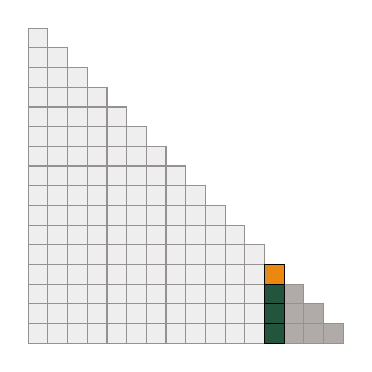
\begin{tikzpicture}[scale=4/16]
  \filldraw[draw=zeroborder, fill=zerocolor] (0, 0) rectangle (1, -1);
  \filldraw[draw=zeroborder, fill=zerocolor] (0, -1) rectangle (1, -2);
  \filldraw[draw=zeroborder, fill=zerocolor] (0, -2) rectangle (1, -3);
  \filldraw[draw=zeroborder, fill=zerocolor] (0, -3) rectangle (1, -4);
  \filldraw[draw=zeroborder, fill=zerocolor] (0, -4) rectangle (1, -5);
  \filldraw[draw=zeroborder, fill=zerocolor] (0, -5) rectangle (1, -6);
  \filldraw[draw=zeroborder, fill=zerocolor] (0, -6) rectangle (1, -7);
  \filldraw[draw=zeroborder, fill=zerocolor] (0, -7) rectangle (1, -8);
  \filldraw[draw=zeroborder, fill=zerocolor] (0, -8) rectangle (1, -9);
  \filldraw[draw=zeroborder, fill=zerocolor] (0, -9) rectangle (1, -10);
  \filldraw[draw=zeroborder, fill=zerocolor] (0, -10) rectangle (1, -11);
  \filldraw[draw=zeroborder, fill=zerocolor] (0, -11) rectangle (1, -12);
  \filldraw[draw=zeroborder, fill=zerocolor] (0, -12) rectangle (1, -13);
  \filldraw[draw=zeroborder, fill=zerocolor] (0, -13) rectangle (1, -14);
  \filldraw[draw=zeroborder, fill=zerocolor] (0, -14) rectangle (1, -15);
  \filldraw[draw=zeroborder, fill=zerocolor] (0, -15) rectangle (1, -16);
  \filldraw[draw=zeroborder, fill=zerocolor] (1, -1) rectangle (2, -2);
  \filldraw[draw=zeroborder, fill=zerocolor] (1, -2) rectangle (2, -3);
  \filldraw[draw=zeroborder, fill=zerocolor] (1, -3) rectangle (2, -4);
  \filldraw[draw=zeroborder, fill=zerocolor] (1, -4) rectangle (2, -5);
  \filldraw[draw=zeroborder, fill=zerocolor] (1, -5) rectangle (2, -6);
  \filldraw[draw=zeroborder, fill=zerocolor] (1, -6) rectangle (2, -7);
  \filldraw[draw=zeroborder, fill=zerocolor] (1, -7) rectangle (2, -8);
  \filldraw[draw=zeroborder, fill=zerocolor] (1, -8) rectangle (2, -9);
  \filldraw[draw=zeroborder, fill=zerocolor] (1, -9) rectangle (2, -10);
  \filldraw[draw=zeroborder, fill=zerocolor] (1, -10) rectangle (2, -11);
  \filldraw[draw=zeroborder, fill=zerocolor] (1, -11) rectangle (2, -12);
  \filldraw[draw=zeroborder, fill=zerocolor] (1, -12) rectangle (2, -13);
  \filldraw[draw=zeroborder, fill=zerocolor] (1, -13) rectangle (2, -14);
  \filldraw[draw=zeroborder, fill=zerocolor] (1, -14) rectangle (2, -15);
  \filldraw[draw=zeroborder, fill=zerocolor] (1, -15) rectangle (2, -16);
  \filldraw[draw=zeroborder, fill=zerocolor] (2, -2) rectangle (3, -3);
  \filldraw[draw=zeroborder, fill=zerocolor] (2, -3) rectangle (3, -4);
  \filldraw[draw=zeroborder, fill=zerocolor] (2, -4) rectangle (3, -5);
  \filldraw[draw=zeroborder, fill=zerocolor] (2, -5) rectangle (3, -6);
  \filldraw[draw=zeroborder, fill=zerocolor] (2, -6) rectangle (3, -7);
  \filldraw[draw=zeroborder, fill=zerocolor] (2, -7) rectangle (3, -8);
  \filldraw[draw=zeroborder, fill=zerocolor] (2, -8) rectangle (3, -9);
  \filldraw[draw=zeroborder, fill=zerocolor] (2, -9) rectangle (3, -10);
  \filldraw[draw=zeroborder, fill=zerocolor] (2, -10) rectangle (3, -11);
  \filldraw[draw=zeroborder, fill=zerocolor] (2, -11) rectangle (3, -12);
  \filldraw[draw=zeroborder, fill=zerocolor] (2, -12) rectangle (3, -13);
  \filldraw[draw=zeroborder, fill=zerocolor] (2, -13) rectangle (3, -14);
  \filldraw[draw=zeroborder, fill=zerocolor] (2, -14) rectangle (3, -15);
  \filldraw[draw=zeroborder, fill=zerocolor] (2, -15) rectangle (3, -16);
  \filldraw[draw=zeroborder, fill=zerocolor] (3, -3) rectangle (4, -4);
  \filldraw[draw=zeroborder, fill=zerocolor] (3, -4) rectangle (4, -5);
  \filldraw[draw=zeroborder, fill=zerocolor] (3, -5) rectangle (4, -6);
  \filldraw[draw=zeroborder, fill=zerocolor] (3, -6) rectangle (4, -7);
  \filldraw[draw=zeroborder, fill=zerocolor] (3, -7) rectangle (4, -8);
  \filldraw[draw=zeroborder, fill=zerocolor] (3, -8) rectangle (4, -9);
  \filldraw[draw=zeroborder, fill=zerocolor] (3, -9) rectangle (4, -10);
  \filldraw[draw=zeroborder, fill=zerocolor] (3, -10) rectangle (4, -11);
  \filldraw[draw=zeroborder, fill=zerocolor] (3, -11) rectangle (4, -12);
  \filldraw[draw=zeroborder, fill=zerocolor] (3, -12) rectangle (4, -13);
  \filldraw[draw=zeroborder, fill=zerocolor] (3, -13) rectangle (4, -14);
  \filldraw[draw=zeroborder, fill=zerocolor] (3, -14) rectangle (4, -15);
  \filldraw[draw=zeroborder, fill=zerocolor] (3, -15) rectangle (4, -16);
  \filldraw[draw=zeroborder, fill=zerocolor] (4, -4) rectangle (5, -5);
  \filldraw[draw=zeroborder, fill=zerocolor] (4, -5) rectangle (5, -6);
  \filldraw[draw=zeroborder, fill=zerocolor] (4, -6) rectangle (5, -7);
  \filldraw[draw=zeroborder, fill=zerocolor] (4, -7) rectangle (5, -8);
  \filldraw[draw=zeroborder, fill=zerocolor] (4, -8) rectangle (5, -9);
  \filldraw[draw=zeroborder, fill=zerocolor] (4, -9) rectangle (5, -10);
  \filldraw[draw=zeroborder, fill=zerocolor] (4, -10) rectangle (5, -11);
  \filldraw[draw=zeroborder, fill=zerocolor] (4, -11) rectangle (5, -12);
  \filldraw[draw=zeroborder, fill=zerocolor] (4, -12) rectangle (5, -13);
  \filldraw[draw=zeroborder, fill=zerocolor] (4, -13) rectangle (5, -14);
  \filldraw[draw=zeroborder, fill=zerocolor] (4, -14) rectangle (5, -15);
  \filldraw[draw=zeroborder, fill=zerocolor] (4, -15) rectangle (5, -16);
  \filldraw[draw=zeroborder, fill=zerocolor] (5, -5) rectangle (6, -6);
  \filldraw[draw=zeroborder, fill=zerocolor] (5, -6) rectangle (6, -7);
  \filldraw[draw=zeroborder, fill=zerocolor] (5, -7) rectangle (6, -8);
  \filldraw[draw=zeroborder, fill=zerocolor] (5, -8) rectangle (6, -9);
  \filldraw[draw=zeroborder, fill=zerocolor] (5, -9) rectangle (6, -10);
  \filldraw[draw=zeroborder, fill=zerocolor] (5, -10) rectangle (6, -11);
  \filldraw[draw=zeroborder, fill=zerocolor] (5, -11) rectangle (6, -12);
  \filldraw[draw=zeroborder, fill=zerocolor] (5, -12) rectangle (6, -13);
  \filldraw[draw=zeroborder, fill=zerocolor] (5, -13) rectangle (6, -14);
  \filldraw[draw=zeroborder, fill=zerocolor] (5, -14) rectangle (6, -15);
  \filldraw[draw=zeroborder, fill=zerocolor] (5, -15) rectangle (6, -16);
  \filldraw[draw=zeroborder, fill=zerocolor] (6, -6) rectangle (7, -7);
  \filldraw[draw=zeroborder, fill=zerocolor] (6, -7) rectangle (7, -8);
  \filldraw[draw=zeroborder, fill=zerocolor] (6, -8) rectangle (7, -9);
  \filldraw[draw=zeroborder, fill=zerocolor] (6, -9) rectangle (7, -10);
  \filldraw[draw=zeroborder, fill=zerocolor] (6, -10) rectangle (7, -11);
  \filldraw[draw=zeroborder, fill=zerocolor] (6, -11) rectangle (7, -12);
  \filldraw[draw=zeroborder, fill=zerocolor] (6, -12) rectangle (7, -13);
  \filldraw[draw=zeroborder, fill=zerocolor] (6, -13) rectangle (7, -14);
  \filldraw[draw=zeroborder, fill=zerocolor] (6, -14) rectangle (7, -15);
  \filldraw[draw=zeroborder, fill=zerocolor] (6, -15) rectangle (7, -16);
  \filldraw[draw=zeroborder, fill=zerocolor] (7, -7) rectangle (8, -8);
  \filldraw[draw=zeroborder, fill=zerocolor] (7, -8) rectangle (8, -9);
  \filldraw[draw=zeroborder, fill=zerocolor] (7, -9) rectangle (8, -10);
  \filldraw[draw=zeroborder, fill=zerocolor] (7, -10) rectangle (8, -11);
  \filldraw[draw=zeroborder, fill=zerocolor] (7, -11) rectangle (8, -12);
  \filldraw[draw=zeroborder, fill=zerocolor] (7, -12) rectangle (8, -13);
  \filldraw[draw=zeroborder, fill=zerocolor] (7, -13) rectangle (8, -14);
  \filldraw[draw=zeroborder, fill=zerocolor] (7, -14) rectangle (8, -15);
  \filldraw[draw=zeroborder, fill=zerocolor] (7, -15) rectangle (8, -16);
  \filldraw[draw=zeroborder, fill=zerocolor] (8, -8) rectangle (9, -9);
  \filldraw[draw=zeroborder, fill=zerocolor] (8, -9) rectangle (9, -10);
  \filldraw[draw=zeroborder, fill=zerocolor] (8, -10) rectangle (9, -11);
  \filldraw[draw=zeroborder, fill=zerocolor] (8, -11) rectangle (9, -12);
  \filldraw[draw=zeroborder, fill=zerocolor] (8, -12) rectangle (9, -13);
  \filldraw[draw=zeroborder, fill=zerocolor] (8, -13) rectangle (9, -14);
  \filldraw[draw=zeroborder, fill=zerocolor] (8, -14) rectangle (9, -15);
  \filldraw[draw=zeroborder, fill=zerocolor] (8, -15) rectangle (9, -16);
  \filldraw[draw=zeroborder, fill=zerocolor] (9, -9) rectangle (10, -10);
  \filldraw[draw=zeroborder, fill=zerocolor] (9, -10) rectangle (10, -11);
  \filldraw[draw=zeroborder, fill=zerocolor] (9, -11) rectangle (10, -12);
  \filldraw[draw=zeroborder, fill=zerocolor] (9, -12) rectangle (10, -13);
  \filldraw[draw=zeroborder, fill=zerocolor] (9, -13) rectangle (10, -14);
  \filldraw[draw=zeroborder, fill=zerocolor] (9, -14) rectangle (10, -15);
  \filldraw[draw=zeroborder, fill=zerocolor] (9, -15) rectangle (10, -16);
  \filldraw[draw=zeroborder, fill=zerocolor] (10, -10) rectangle (11, -11);
  \filldraw[draw=zeroborder, fill=zerocolor] (10, -11) rectangle (11, -12);
  \filldraw[draw=zeroborder, fill=zerocolor] (10, -12) rectangle (11, -13);
  \filldraw[draw=zeroborder, fill=zerocolor] (10, -13) rectangle (11, -14);
  \filldraw[draw=zeroborder, fill=zerocolor] (10, -14) rectangle (11, -15);
  \filldraw[draw=zeroborder, fill=zerocolor] (10, -15) rectangle (11, -16);
  \filldraw[draw=zeroborder, fill=zerocolor] (11, -11) rectangle (12, -12);
  \filldraw[draw=zeroborder, fill=zerocolor] (11, -12) rectangle (12, -13);
  \filldraw[draw=zeroborder, fill=zerocolor] (11, -13) rectangle (12, -14);
  \filldraw[draw=zeroborder, fill=zerocolor] (11, -14) rectangle (12, -15);
  \filldraw[draw=zeroborder, fill=zerocolor] (11, -15) rectangle (12, -16);
  \filldraw[draw=nnzborder, fill=nnzcolor] (13, -13) rectangle (14, -14);
  \filldraw[draw=nnzborder, fill=nnzcolor] (13, -14) rectangle (14, -15);
  \filldraw[draw=nnzborder, fill=nnzcolor] (13, -15) rectangle (14, -16);
  \filldraw[draw=nnzborder, fill=nnzcolor] (14, -14) rectangle (15, -15);
  \filldraw[draw=nnzborder, fill=nnzcolor] (14, -15) rectangle (15, -16);
  \filldraw[draw=nnzborder, fill=nnzcolor] (15, -15) rectangle (16, -16);
  \filldraw[draw=colborder, fill=targetcolor] (12, -12) rectangle (13, -13);
  \filldraw[draw=colborder, fill=selcolor] (12, -13) rectangle (13, -14);
  \filldraw[draw=colborder, fill=selcolor] (12, -14) rectangle (13, -15);
  \filldraw[draw=colborder, fill=selcolor] (12, -15) rectangle (13, -16);
\end{tikzpicture}
%
    \qquad
    \begin{tikzpicture}[baseline]
  \begin{axis}[
    % calculated from Cholesky factor, exactly 16 cm x 16 cm
    width={4cm},
    height={4cm},
    axis lines={none},
    % force axis box to have exactly the right dimensions, ignoring labels
    scale only axis=true,
  ]
  % consistent size bounding box
  \draw [white, line width=0] (-0.1, -0.1) -- (-0.1,  1.1);
  \draw [white, line width=0] ( 1.1, -0.1) -- ( 1.1,  1.1);
  \draw [white, line width=0] (-0.1, -0.1) -- (-1.1, -0.1);
  \draw [white, line width=0] (-0.1,  1.1) -- (-1.1,  1.1);
  \draw [seagreen!15, fill, radius=1.3210153579711914] (0.7345771514092145, 0.11367201992140341) circle;
  \draw [seagreen, radius=1.3210153579711914] (0.7345771514092145, 0.11367201992140341) circle;
  \draw [orange!25, fill, radius=0.6605076789855957] (0.7345771514092145, 0.11367201992140341) circle;
  \draw [orange, radius=0.6605076789855957] (0.7345771514092145, 0.11367201992140341) circle;
  \addplot [only marks, mark size=1, silver]    table
    {figures/points_knn/all_points.csv};
  \addplot [only marks, mark size=2, lightblue] table
    {figures/points_knn/candidates_04.csv};
  \addplot [only marks, mark size=4, seagreen]  table
    {figures/points_knn/selected_04.csv};
  \addplot [only marks, mark size=4, orange]    table
    {figures/points_knn/target_04.csv};
  \end{axis}
\end{tikzpicture}

  \end{figure}
}
\only<5>{
  \begin{figure}
    \centering
    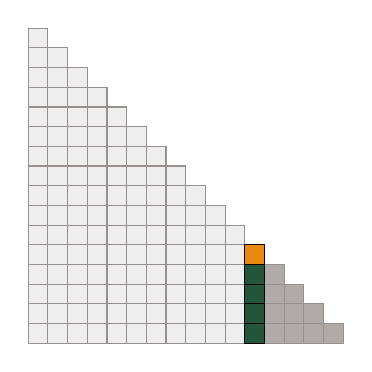
\begin{tikzpicture}[scale=4/16]
  \filldraw[draw=zeroborder, fill=zerocolor] (0, 0) rectangle (1, -1);
  \filldraw[draw=zeroborder, fill=zerocolor] (0, -1) rectangle (1, -2);
  \filldraw[draw=zeroborder, fill=zerocolor] (0, -2) rectangle (1, -3);
  \filldraw[draw=zeroborder, fill=zerocolor] (0, -3) rectangle (1, -4);
  \filldraw[draw=zeroborder, fill=zerocolor] (0, -4) rectangle (1, -5);
  \filldraw[draw=zeroborder, fill=zerocolor] (0, -5) rectangle (1, -6);
  \filldraw[draw=zeroborder, fill=zerocolor] (0, -6) rectangle (1, -7);
  \filldraw[draw=zeroborder, fill=zerocolor] (0, -7) rectangle (1, -8);
  \filldraw[draw=zeroborder, fill=zerocolor] (0, -8) rectangle (1, -9);
  \filldraw[draw=zeroborder, fill=zerocolor] (0, -9) rectangle (1, -10);
  \filldraw[draw=zeroborder, fill=zerocolor] (0, -10) rectangle (1, -11);
  \filldraw[draw=zeroborder, fill=zerocolor] (0, -11) rectangle (1, -12);
  \filldraw[draw=zeroborder, fill=zerocolor] (0, -12) rectangle (1, -13);
  \filldraw[draw=zeroborder, fill=zerocolor] (0, -13) rectangle (1, -14);
  \filldraw[draw=zeroborder, fill=zerocolor] (0, -14) rectangle (1, -15);
  \filldraw[draw=zeroborder, fill=zerocolor] (0, -15) rectangle (1, -16);
  \filldraw[draw=zeroborder, fill=zerocolor] (1, -1) rectangle (2, -2);
  \filldraw[draw=zeroborder, fill=zerocolor] (1, -2) rectangle (2, -3);
  \filldraw[draw=zeroborder, fill=zerocolor] (1, -3) rectangle (2, -4);
  \filldraw[draw=zeroborder, fill=zerocolor] (1, -4) rectangle (2, -5);
  \filldraw[draw=zeroborder, fill=zerocolor] (1, -5) rectangle (2, -6);
  \filldraw[draw=zeroborder, fill=zerocolor] (1, -6) rectangle (2, -7);
  \filldraw[draw=zeroborder, fill=zerocolor] (1, -7) rectangle (2, -8);
  \filldraw[draw=zeroborder, fill=zerocolor] (1, -8) rectangle (2, -9);
  \filldraw[draw=zeroborder, fill=zerocolor] (1, -9) rectangle (2, -10);
  \filldraw[draw=zeroborder, fill=zerocolor] (1, -10) rectangle (2, -11);
  \filldraw[draw=zeroborder, fill=zerocolor] (1, -11) rectangle (2, -12);
  \filldraw[draw=zeroborder, fill=zerocolor] (1, -12) rectangle (2, -13);
  \filldraw[draw=zeroborder, fill=zerocolor] (1, -13) rectangle (2, -14);
  \filldraw[draw=zeroborder, fill=zerocolor] (1, -14) rectangle (2, -15);
  \filldraw[draw=zeroborder, fill=zerocolor] (1, -15) rectangle (2, -16);
  \filldraw[draw=zeroborder, fill=zerocolor] (2, -2) rectangle (3, -3);
  \filldraw[draw=zeroborder, fill=zerocolor] (2, -3) rectangle (3, -4);
  \filldraw[draw=zeroborder, fill=zerocolor] (2, -4) rectangle (3, -5);
  \filldraw[draw=zeroborder, fill=zerocolor] (2, -5) rectangle (3, -6);
  \filldraw[draw=zeroborder, fill=zerocolor] (2, -6) rectangle (3, -7);
  \filldraw[draw=zeroborder, fill=zerocolor] (2, -7) rectangle (3, -8);
  \filldraw[draw=zeroborder, fill=zerocolor] (2, -8) rectangle (3, -9);
  \filldraw[draw=zeroborder, fill=zerocolor] (2, -9) rectangle (3, -10);
  \filldraw[draw=zeroborder, fill=zerocolor] (2, -10) rectangle (3, -11);
  \filldraw[draw=zeroborder, fill=zerocolor] (2, -11) rectangle (3, -12);
  \filldraw[draw=zeroborder, fill=zerocolor] (2, -12) rectangle (3, -13);
  \filldraw[draw=zeroborder, fill=zerocolor] (2, -13) rectangle (3, -14);
  \filldraw[draw=zeroborder, fill=zerocolor] (2, -14) rectangle (3, -15);
  \filldraw[draw=zeroborder, fill=zerocolor] (2, -15) rectangle (3, -16);
  \filldraw[draw=zeroborder, fill=zerocolor] (3, -3) rectangle (4, -4);
  \filldraw[draw=zeroborder, fill=zerocolor] (3, -4) rectangle (4, -5);
  \filldraw[draw=zeroborder, fill=zerocolor] (3, -5) rectangle (4, -6);
  \filldraw[draw=zeroborder, fill=zerocolor] (3, -6) rectangle (4, -7);
  \filldraw[draw=zeroborder, fill=zerocolor] (3, -7) rectangle (4, -8);
  \filldraw[draw=zeroborder, fill=zerocolor] (3, -8) rectangle (4, -9);
  \filldraw[draw=zeroborder, fill=zerocolor] (3, -9) rectangle (4, -10);
  \filldraw[draw=zeroborder, fill=zerocolor] (3, -10) rectangle (4, -11);
  \filldraw[draw=zeroborder, fill=zerocolor] (3, -11) rectangle (4, -12);
  \filldraw[draw=zeroborder, fill=zerocolor] (3, -12) rectangle (4, -13);
  \filldraw[draw=zeroborder, fill=zerocolor] (3, -13) rectangle (4, -14);
  \filldraw[draw=zeroborder, fill=zerocolor] (3, -14) rectangle (4, -15);
  \filldraw[draw=zeroborder, fill=zerocolor] (3, -15) rectangle (4, -16);
  \filldraw[draw=zeroborder, fill=zerocolor] (4, -4) rectangle (5, -5);
  \filldraw[draw=zeroborder, fill=zerocolor] (4, -5) rectangle (5, -6);
  \filldraw[draw=zeroborder, fill=zerocolor] (4, -6) rectangle (5, -7);
  \filldraw[draw=zeroborder, fill=zerocolor] (4, -7) rectangle (5, -8);
  \filldraw[draw=zeroborder, fill=zerocolor] (4, -8) rectangle (5, -9);
  \filldraw[draw=zeroborder, fill=zerocolor] (4, -9) rectangle (5, -10);
  \filldraw[draw=zeroborder, fill=zerocolor] (4, -10) rectangle (5, -11);
  \filldraw[draw=zeroborder, fill=zerocolor] (4, -11) rectangle (5, -12);
  \filldraw[draw=zeroborder, fill=zerocolor] (4, -12) rectangle (5, -13);
  \filldraw[draw=zeroborder, fill=zerocolor] (4, -13) rectangle (5, -14);
  \filldraw[draw=zeroborder, fill=zerocolor] (4, -14) rectangle (5, -15);
  \filldraw[draw=zeroborder, fill=zerocolor] (4, -15) rectangle (5, -16);
  \filldraw[draw=zeroborder, fill=zerocolor] (5, -5) rectangle (6, -6);
  \filldraw[draw=zeroborder, fill=zerocolor] (5, -6) rectangle (6, -7);
  \filldraw[draw=zeroborder, fill=zerocolor] (5, -7) rectangle (6, -8);
  \filldraw[draw=zeroborder, fill=zerocolor] (5, -8) rectangle (6, -9);
  \filldraw[draw=zeroborder, fill=zerocolor] (5, -9) rectangle (6, -10);
  \filldraw[draw=zeroborder, fill=zerocolor] (5, -10) rectangle (6, -11);
  \filldraw[draw=zeroborder, fill=zerocolor] (5, -11) rectangle (6, -12);
  \filldraw[draw=zeroborder, fill=zerocolor] (5, -12) rectangle (6, -13);
  \filldraw[draw=zeroborder, fill=zerocolor] (5, -13) rectangle (6, -14);
  \filldraw[draw=zeroborder, fill=zerocolor] (5, -14) rectangle (6, -15);
  \filldraw[draw=zeroborder, fill=zerocolor] (5, -15) rectangle (6, -16);
  \filldraw[draw=zeroborder, fill=zerocolor] (6, -6) rectangle (7, -7);
  \filldraw[draw=zeroborder, fill=zerocolor] (6, -7) rectangle (7, -8);
  \filldraw[draw=zeroborder, fill=zerocolor] (6, -8) rectangle (7, -9);
  \filldraw[draw=zeroborder, fill=zerocolor] (6, -9) rectangle (7, -10);
  \filldraw[draw=zeroborder, fill=zerocolor] (6, -10) rectangle (7, -11);
  \filldraw[draw=zeroborder, fill=zerocolor] (6, -11) rectangle (7, -12);
  \filldraw[draw=zeroborder, fill=zerocolor] (6, -12) rectangle (7, -13);
  \filldraw[draw=zeroborder, fill=zerocolor] (6, -13) rectangle (7, -14);
  \filldraw[draw=zeroborder, fill=zerocolor] (6, -14) rectangle (7, -15);
  \filldraw[draw=zeroborder, fill=zerocolor] (6, -15) rectangle (7, -16);
  \filldraw[draw=zeroborder, fill=zerocolor] (7, -7) rectangle (8, -8);
  \filldraw[draw=zeroborder, fill=zerocolor] (7, -8) rectangle (8, -9);
  \filldraw[draw=zeroborder, fill=zerocolor] (7, -9) rectangle (8, -10);
  \filldraw[draw=zeroborder, fill=zerocolor] (7, -10) rectangle (8, -11);
  \filldraw[draw=zeroborder, fill=zerocolor] (7, -11) rectangle (8, -12);
  \filldraw[draw=zeroborder, fill=zerocolor] (7, -12) rectangle (8, -13);
  \filldraw[draw=zeroborder, fill=zerocolor] (7, -13) rectangle (8, -14);
  \filldraw[draw=zeroborder, fill=zerocolor] (7, -14) rectangle (8, -15);
  \filldraw[draw=zeroborder, fill=zerocolor] (7, -15) rectangle (8, -16);
  \filldraw[draw=zeroborder, fill=zerocolor] (8, -8) rectangle (9, -9);
  \filldraw[draw=zeroborder, fill=zerocolor] (8, -9) rectangle (9, -10);
  \filldraw[draw=zeroborder, fill=zerocolor] (8, -10) rectangle (9, -11);
  \filldraw[draw=zeroborder, fill=zerocolor] (8, -11) rectangle (9, -12);
  \filldraw[draw=zeroborder, fill=zerocolor] (8, -12) rectangle (9, -13);
  \filldraw[draw=zeroborder, fill=zerocolor] (8, -13) rectangle (9, -14);
  \filldraw[draw=zeroborder, fill=zerocolor] (8, -14) rectangle (9, -15);
  \filldraw[draw=zeroborder, fill=zerocolor] (8, -15) rectangle (9, -16);
  \filldraw[draw=zeroborder, fill=zerocolor] (9, -9) rectangle (10, -10);
  \filldraw[draw=zeroborder, fill=zerocolor] (9, -10) rectangle (10, -11);
  \filldraw[draw=zeroborder, fill=zerocolor] (9, -11) rectangle (10, -12);
  \filldraw[draw=zeroborder, fill=zerocolor] (9, -12) rectangle (10, -13);
  \filldraw[draw=zeroborder, fill=zerocolor] (9, -13) rectangle (10, -14);
  \filldraw[draw=zeroborder, fill=zerocolor] (9, -14) rectangle (10, -15);
  \filldraw[draw=zeroborder, fill=zerocolor] (9, -15) rectangle (10, -16);
  \filldraw[draw=zeroborder, fill=zerocolor] (10, -10) rectangle (11, -11);
  \filldraw[draw=zeroborder, fill=zerocolor] (10, -11) rectangle (11, -12);
  \filldraw[draw=zeroborder, fill=zerocolor] (10, -12) rectangle (11, -13);
  \filldraw[draw=zeroborder, fill=zerocolor] (10, -13) rectangle (11, -14);
  \filldraw[draw=zeroborder, fill=zerocolor] (10, -14) rectangle (11, -15);
  \filldraw[draw=zeroborder, fill=zerocolor] (10, -15) rectangle (11, -16);
  \filldraw[draw=nnzborder, fill=nnzcolor] (12, -12) rectangle (13, -13);
  \filldraw[draw=nnzborder, fill=nnzcolor] (12, -13) rectangle (13, -14);
  \filldraw[draw=nnzborder, fill=nnzcolor] (12, -14) rectangle (13, -15);
  \filldraw[draw=nnzborder, fill=nnzcolor] (12, -15) rectangle (13, -16);
  \filldraw[draw=nnzborder, fill=nnzcolor] (13, -13) rectangle (14, -14);
  \filldraw[draw=nnzborder, fill=nnzcolor] (13, -14) rectangle (14, -15);
  \filldraw[draw=nnzborder, fill=nnzcolor] (13, -15) rectangle (14, -16);
  \filldraw[draw=nnzborder, fill=nnzcolor] (14, -14) rectangle (15, -15);
  \filldraw[draw=nnzborder, fill=nnzcolor] (14, -15) rectangle (15, -16);
  \filldraw[draw=nnzborder, fill=nnzcolor] (15, -15) rectangle (16, -16);
  \filldraw[draw=colborder, fill=targetcolor] (11, -11) rectangle (12, -12);
  \filldraw[draw=colborder, fill=selcolor] (11, -12) rectangle (12, -13);
  \filldraw[draw=colborder, fill=selcolor] (11, -13) rectangle (12, -14);
  \filldraw[draw=colborder, fill=selcolor] (11, -14) rectangle (12, -15);
  \filldraw[draw=colborder, fill=selcolor] (11, -15) rectangle (12, -16);
\end{tikzpicture}
%
    \qquad
    \begin{tikzpicture}[baseline]
  \begin{axis}[
    % calculated from Cholesky factor, exactly 16 cm x 16 cm
    width={4cm},
    height={4cm},
    axis lines={none},
    % force axis box to have exactly the right dimensions, ignoring labels
    scale only axis=true,
  ]
  % consistent size bounding box
  \draw [white, line width=0] (-0.1, -0.1) -- (-0.1,  1.1);
  \draw [white, line width=0] ( 1.1, -0.1) -- ( 1.1,  1.1);
  \draw [white, line width=0] (-0.1, -0.1) -- (-1.1, -0.1);
  \draw [white, line width=0] (-0.1,  1.1) -- (-1.1,  1.1);
  \addplot [only marks, mark size=1, silver]    table
    {figures/points_cknn/all_points.csv};
  \addplot [only marks, mark size=2, lightblue] table
    {figures/points_cknn/candidates.csv};
  \addplot [only marks, mark size=4, seagreen]  table
    {figures/points_cknn/selected_05.csv};
  \addplot [only marks, mark size=4, orange]    table
    {figures/points_cknn/target.csv};
  \end{axis}
\end{tikzpicture}

  \end{figure}
}
\only<6>{
  \begin{figure}
    \centering
    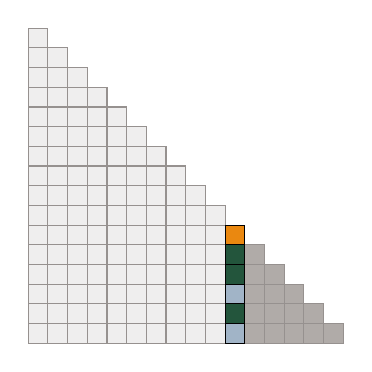
\begin{tikzpicture}[scale=4/16]
  \filldraw[draw=zeroborder, fill=zerocolor] (0, 0) rectangle (1, -1);
  \filldraw[draw=zeroborder, fill=zerocolor] (0, -1) rectangle (1, -2);
  \filldraw[draw=zeroborder, fill=zerocolor] (0, -2) rectangle (1, -3);
  \filldraw[draw=zeroborder, fill=zerocolor] (0, -3) rectangle (1, -4);
  \filldraw[draw=zeroborder, fill=zerocolor] (0, -4) rectangle (1, -5);
  \filldraw[draw=zeroborder, fill=zerocolor] (0, -5) rectangle (1, -6);
  \filldraw[draw=zeroborder, fill=zerocolor] (0, -6) rectangle (1, -7);
  \filldraw[draw=zeroborder, fill=zerocolor] (0, -7) rectangle (1, -8);
  \filldraw[draw=zeroborder, fill=zerocolor] (0, -8) rectangle (1, -9);
  \filldraw[draw=zeroborder, fill=zerocolor] (0, -9) rectangle (1, -10);
  \filldraw[draw=zeroborder, fill=zerocolor] (0, -10) rectangle (1, -11);
  \filldraw[draw=zeroborder, fill=zerocolor] (0, -11) rectangle (1, -12);
  \filldraw[draw=zeroborder, fill=zerocolor] (0, -12) rectangle (1, -13);
  \filldraw[draw=zeroborder, fill=zerocolor] (0, -13) rectangle (1, -14);
  \filldraw[draw=zeroborder, fill=zerocolor] (0, -14) rectangle (1, -15);
  \filldraw[draw=zeroborder, fill=zerocolor] (0, -15) rectangle (1, -16);
  \filldraw[draw=zeroborder, fill=zerocolor] (1, -1) rectangle (2, -2);
  \filldraw[draw=zeroborder, fill=zerocolor] (1, -2) rectangle (2, -3);
  \filldraw[draw=zeroborder, fill=zerocolor] (1, -3) rectangle (2, -4);
  \filldraw[draw=zeroborder, fill=zerocolor] (1, -4) rectangle (2, -5);
  \filldraw[draw=zeroborder, fill=zerocolor] (1, -5) rectangle (2, -6);
  \filldraw[draw=zeroborder, fill=zerocolor] (1, -6) rectangle (2, -7);
  \filldraw[draw=zeroborder, fill=zerocolor] (1, -7) rectangle (2, -8);
  \filldraw[draw=zeroborder, fill=zerocolor] (1, -8) rectangle (2, -9);
  \filldraw[draw=zeroborder, fill=zerocolor] (1, -9) rectangle (2, -10);
  \filldraw[draw=zeroborder, fill=zerocolor] (1, -10) rectangle (2, -11);
  \filldraw[draw=zeroborder, fill=zerocolor] (1, -11) rectangle (2, -12);
  \filldraw[draw=zeroborder, fill=zerocolor] (1, -12) rectangle (2, -13);
  \filldraw[draw=zeroborder, fill=zerocolor] (1, -13) rectangle (2, -14);
  \filldraw[draw=zeroborder, fill=zerocolor] (1, -14) rectangle (2, -15);
  \filldraw[draw=zeroborder, fill=zerocolor] (1, -15) rectangle (2, -16);
  \filldraw[draw=zeroborder, fill=zerocolor] (2, -2) rectangle (3, -3);
  \filldraw[draw=zeroborder, fill=zerocolor] (2, -3) rectangle (3, -4);
  \filldraw[draw=zeroborder, fill=zerocolor] (2, -4) rectangle (3, -5);
  \filldraw[draw=zeroborder, fill=zerocolor] (2, -5) rectangle (3, -6);
  \filldraw[draw=zeroborder, fill=zerocolor] (2, -6) rectangle (3, -7);
  \filldraw[draw=zeroborder, fill=zerocolor] (2, -7) rectangle (3, -8);
  \filldraw[draw=zeroborder, fill=zerocolor] (2, -8) rectangle (3, -9);
  \filldraw[draw=zeroborder, fill=zerocolor] (2, -9) rectangle (3, -10);
  \filldraw[draw=zeroborder, fill=zerocolor] (2, -10) rectangle (3, -11);
  \filldraw[draw=zeroborder, fill=zerocolor] (2, -11) rectangle (3, -12);
  \filldraw[draw=zeroborder, fill=zerocolor] (2, -12) rectangle (3, -13);
  \filldraw[draw=zeroborder, fill=zerocolor] (2, -13) rectangle (3, -14);
  \filldraw[draw=zeroborder, fill=zerocolor] (2, -14) rectangle (3, -15);
  \filldraw[draw=zeroborder, fill=zerocolor] (2, -15) rectangle (3, -16);
  \filldraw[draw=zeroborder, fill=zerocolor] (3, -3) rectangle (4, -4);
  \filldraw[draw=zeroborder, fill=zerocolor] (3, -4) rectangle (4, -5);
  \filldraw[draw=zeroborder, fill=zerocolor] (3, -5) rectangle (4, -6);
  \filldraw[draw=zeroborder, fill=zerocolor] (3, -6) rectangle (4, -7);
  \filldraw[draw=zeroborder, fill=zerocolor] (3, -7) rectangle (4, -8);
  \filldraw[draw=zeroborder, fill=zerocolor] (3, -8) rectangle (4, -9);
  \filldraw[draw=zeroborder, fill=zerocolor] (3, -9) rectangle (4, -10);
  \filldraw[draw=zeroborder, fill=zerocolor] (3, -10) rectangle (4, -11);
  \filldraw[draw=zeroborder, fill=zerocolor] (3, -11) rectangle (4, -12);
  \filldraw[draw=zeroborder, fill=zerocolor] (3, -12) rectangle (4, -13);
  \filldraw[draw=zeroborder, fill=zerocolor] (3, -13) rectangle (4, -14);
  \filldraw[draw=zeroborder, fill=zerocolor] (3, -14) rectangle (4, -15);
  \filldraw[draw=zeroborder, fill=zerocolor] (3, -15) rectangle (4, -16);
  \filldraw[draw=zeroborder, fill=zerocolor] (4, -4) rectangle (5, -5);
  \filldraw[draw=zeroborder, fill=zerocolor] (4, -5) rectangle (5, -6);
  \filldraw[draw=zeroborder, fill=zerocolor] (4, -6) rectangle (5, -7);
  \filldraw[draw=zeroborder, fill=zerocolor] (4, -7) rectangle (5, -8);
  \filldraw[draw=zeroborder, fill=zerocolor] (4, -8) rectangle (5, -9);
  \filldraw[draw=zeroborder, fill=zerocolor] (4, -9) rectangle (5, -10);
  \filldraw[draw=zeroborder, fill=zerocolor] (4, -10) rectangle (5, -11);
  \filldraw[draw=zeroborder, fill=zerocolor] (4, -11) rectangle (5, -12);
  \filldraw[draw=zeroborder, fill=zerocolor] (4, -12) rectangle (5, -13);
  \filldraw[draw=zeroborder, fill=zerocolor] (4, -13) rectangle (5, -14);
  \filldraw[draw=zeroborder, fill=zerocolor] (4, -14) rectangle (5, -15);
  \filldraw[draw=zeroborder, fill=zerocolor] (4, -15) rectangle (5, -16);
  \filldraw[draw=zeroborder, fill=zerocolor] (5, -5) rectangle (6, -6);
  \filldraw[draw=zeroborder, fill=zerocolor] (5, -6) rectangle (6, -7);
  \filldraw[draw=zeroborder, fill=zerocolor] (5, -7) rectangle (6, -8);
  \filldraw[draw=zeroborder, fill=zerocolor] (5, -8) rectangle (6, -9);
  \filldraw[draw=zeroborder, fill=zerocolor] (5, -9) rectangle (6, -10);
  \filldraw[draw=zeroborder, fill=zerocolor] (5, -10) rectangle (6, -11);
  \filldraw[draw=zeroborder, fill=zerocolor] (5, -11) rectangle (6, -12);
  \filldraw[draw=zeroborder, fill=zerocolor] (5, -12) rectangle (6, -13);
  \filldraw[draw=zeroborder, fill=zerocolor] (5, -13) rectangle (6, -14);
  \filldraw[draw=zeroborder, fill=zerocolor] (5, -14) rectangle (6, -15);
  \filldraw[draw=zeroborder, fill=zerocolor] (5, -15) rectangle (6, -16);
  \filldraw[draw=zeroborder, fill=zerocolor] (6, -6) rectangle (7, -7);
  \filldraw[draw=zeroborder, fill=zerocolor] (6, -7) rectangle (7, -8);
  \filldraw[draw=zeroborder, fill=zerocolor] (6, -8) rectangle (7, -9);
  \filldraw[draw=zeroborder, fill=zerocolor] (6, -9) rectangle (7, -10);
  \filldraw[draw=zeroborder, fill=zerocolor] (6, -10) rectangle (7, -11);
  \filldraw[draw=zeroborder, fill=zerocolor] (6, -11) rectangle (7, -12);
  \filldraw[draw=zeroborder, fill=zerocolor] (6, -12) rectangle (7, -13);
  \filldraw[draw=zeroborder, fill=zerocolor] (6, -13) rectangle (7, -14);
  \filldraw[draw=zeroborder, fill=zerocolor] (6, -14) rectangle (7, -15);
  \filldraw[draw=zeroborder, fill=zerocolor] (6, -15) rectangle (7, -16);
  \filldraw[draw=zeroborder, fill=zerocolor] (7, -7) rectangle (8, -8);
  \filldraw[draw=zeroborder, fill=zerocolor] (7, -8) rectangle (8, -9);
  \filldraw[draw=zeroborder, fill=zerocolor] (7, -9) rectangle (8, -10);
  \filldraw[draw=zeroborder, fill=zerocolor] (7, -10) rectangle (8, -11);
  \filldraw[draw=zeroborder, fill=zerocolor] (7, -11) rectangle (8, -12);
  \filldraw[draw=zeroborder, fill=zerocolor] (7, -12) rectangle (8, -13);
  \filldraw[draw=zeroborder, fill=zerocolor] (7, -13) rectangle (8, -14);
  \filldraw[draw=zeroborder, fill=zerocolor] (7, -14) rectangle (8, -15);
  \filldraw[draw=zeroborder, fill=zerocolor] (7, -15) rectangle (8, -16);
  \filldraw[draw=zeroborder, fill=zerocolor] (8, -8) rectangle (9, -9);
  \filldraw[draw=zeroborder, fill=zerocolor] (8, -9) rectangle (9, -10);
  \filldraw[draw=zeroborder, fill=zerocolor] (8, -10) rectangle (9, -11);
  \filldraw[draw=zeroborder, fill=zerocolor] (8, -11) rectangle (9, -12);
  \filldraw[draw=zeroborder, fill=zerocolor] (8, -12) rectangle (9, -13);
  \filldraw[draw=zeroborder, fill=zerocolor] (8, -13) rectangle (9, -14);
  \filldraw[draw=zeroborder, fill=zerocolor] (8, -14) rectangle (9, -15);
  \filldraw[draw=zeroborder, fill=zerocolor] (8, -15) rectangle (9, -16);
  \filldraw[draw=zeroborder, fill=zerocolor] (9, -9) rectangle (10, -10);
  \filldraw[draw=zeroborder, fill=zerocolor] (9, -10) rectangle (10, -11);
  \filldraw[draw=zeroborder, fill=zerocolor] (9, -11) rectangle (10, -12);
  \filldraw[draw=zeroborder, fill=zerocolor] (9, -12) rectangle (10, -13);
  \filldraw[draw=zeroborder, fill=zerocolor] (9, -13) rectangle (10, -14);
  \filldraw[draw=zeroborder, fill=zerocolor] (9, -14) rectangle (10, -15);
  \filldraw[draw=zeroborder, fill=zerocolor] (9, -15) rectangle (10, -16);
  \filldraw[draw=nnzborder, fill=nnzcolor] (11, -11) rectangle (12, -12);
  \filldraw[draw=nnzborder, fill=nnzcolor] (11, -12) rectangle (12, -13);
  \filldraw[draw=nnzborder, fill=nnzcolor] (11, -13) rectangle (12, -14);
  \filldraw[draw=nnzborder, fill=nnzcolor] (11, -14) rectangle (12, -15);
  \filldraw[draw=nnzborder, fill=nnzcolor] (11, -15) rectangle (12, -16);
  \filldraw[draw=nnzborder, fill=nnzcolor] (12, -12) rectangle (13, -13);
  \filldraw[draw=nnzborder, fill=nnzcolor] (12, -13) rectangle (13, -14);
  \filldraw[draw=nnzborder, fill=nnzcolor] (12, -14) rectangle (13, -15);
  \filldraw[draw=nnzborder, fill=nnzcolor] (12, -15) rectangle (13, -16);
  \filldraw[draw=nnzborder, fill=nnzcolor] (13, -13) rectangle (14, -14);
  \filldraw[draw=nnzborder, fill=nnzcolor] (13, -14) rectangle (14, -15);
  \filldraw[draw=nnzborder, fill=nnzcolor] (13, -15) rectangle (14, -16);
  \filldraw[draw=nnzborder, fill=nnzcolor] (14, -14) rectangle (15, -15);
  \filldraw[draw=nnzborder, fill=nnzcolor] (14, -15) rectangle (15, -16);
  \filldraw[draw=nnzborder, fill=nnzcolor] (15, -15) rectangle (16, -16);
  \filldraw[draw=colborder, fill=targetcolor] (10, -10) rectangle (11, -11);
  \filldraw[draw=colborder, fill=selcolor] (10, -11) rectangle (11, -12);
  \filldraw[draw=colborder, fill=selcolor] (10, -12) rectangle (11, -13);
  \filldraw[draw=colborder, fill=candcolor] (10, -13) rectangle (11, -14);
  \filldraw[draw=colborder, fill=selcolor] (10, -14) rectangle (11, -15);
  \filldraw[draw=colborder, fill=candcolor] (10, -15) rectangle (11, -16);
\end{tikzpicture}
%
    \qquad
    \begin{tikzpicture}[baseline]
  \begin{axis}[
    % calculated from Cholesky factor, exactly 16 cm x 16 cm
    width={4cm},
    height={4cm},
    axis lines={none},
    % force axis box to have exactly the right dimensions, ignoring labels
    scale only axis=true,
  ]
  % consistent size bounding box
  \draw [white, line width=0] (-0.1, -0.1) -- (-0.1,  1.1);
  \draw [white, line width=0] ( 1.1, -0.1) -- ( 1.1,  1.1);
  \draw [white, line width=0] (-0.1, -0.1) -- (-1.1, -0.1);
  \draw [white, line width=0] (-0.1,  1.1) -- (-1.1,  1.1);
  \draw [seagreen!15, fill, radius=0.8034806251525879] (0.8917110704451572, 0.5851629398909081) circle;
  \draw [seagreen, radius=0.8034806251525879] (0.8917110704451572, 0.5851629398909081) circle;
  \draw [orange!25, fill, radius=0.40174031257629395] (0.8917110704451572, 0.5851629398909081) circle;
  \draw [orange, radius=0.40174031257629395] (0.8917110704451572, 0.5851629398909081) circle;
  \addplot [only marks, mark size=1, silver]    table
    {figures/points_knn/all_points.csv};
  \addplot [only marks, mark size=2, lightblue] table
    {figures/points_knn/candidates_06.csv};
  \addplot [only marks, mark size=4, seagreen]  table
    {figures/points_knn/selected_06.csv};
  \addplot [only marks, mark size=4, orange]    table
    {figures/points_knn/target_06.csv};
  \end{axis}
\end{tikzpicture}

  \end{figure}
}
\only<7>{
  \begin{figure}
    \centering
    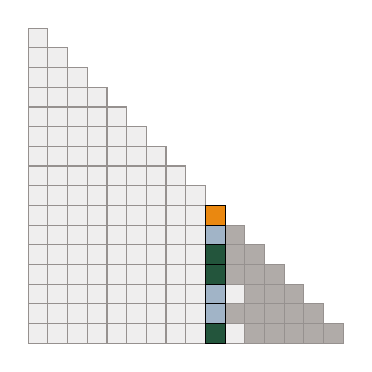
\begin{tikzpicture}[scale=4/16]
  \filldraw[draw=zeroborder, fill=zerocolor] (0, 0) rectangle (1, -1);
  \filldraw[draw=zeroborder, fill=zerocolor] (0, -1) rectangle (1, -2);
  \filldraw[draw=zeroborder, fill=zerocolor] (0, -2) rectangle (1, -3);
  \filldraw[draw=zeroborder, fill=zerocolor] (0, -3) rectangle (1, -4);
  \filldraw[draw=zeroborder, fill=zerocolor] (0, -4) rectangle (1, -5);
  \filldraw[draw=zeroborder, fill=zerocolor] (0, -5) rectangle (1, -6);
  \filldraw[draw=zeroborder, fill=zerocolor] (0, -6) rectangle (1, -7);
  \filldraw[draw=zeroborder, fill=zerocolor] (0, -7) rectangle (1, -8);
  \filldraw[draw=zeroborder, fill=zerocolor] (0, -8) rectangle (1, -9);
  \filldraw[draw=zeroborder, fill=zerocolor] (0, -9) rectangle (1, -10);
  \filldraw[draw=zeroborder, fill=zerocolor] (0, -10) rectangle (1, -11);
  \filldraw[draw=zeroborder, fill=zerocolor] (0, -11) rectangle (1, -12);
  \filldraw[draw=zeroborder, fill=zerocolor] (0, -12) rectangle (1, -13);
  \filldraw[draw=zeroborder, fill=zerocolor] (0, -13) rectangle (1, -14);
  \filldraw[draw=zeroborder, fill=zerocolor] (0, -14) rectangle (1, -15);
  \filldraw[draw=zeroborder, fill=zerocolor] (0, -15) rectangle (1, -16);
  \filldraw[draw=zeroborder, fill=zerocolor] (1, -1) rectangle (2, -2);
  \filldraw[draw=zeroborder, fill=zerocolor] (1, -2) rectangle (2, -3);
  \filldraw[draw=zeroborder, fill=zerocolor] (1, -3) rectangle (2, -4);
  \filldraw[draw=zeroborder, fill=zerocolor] (1, -4) rectangle (2, -5);
  \filldraw[draw=zeroborder, fill=zerocolor] (1, -5) rectangle (2, -6);
  \filldraw[draw=zeroborder, fill=zerocolor] (1, -6) rectangle (2, -7);
  \filldraw[draw=zeroborder, fill=zerocolor] (1, -7) rectangle (2, -8);
  \filldraw[draw=zeroborder, fill=zerocolor] (1, -8) rectangle (2, -9);
  \filldraw[draw=zeroborder, fill=zerocolor] (1, -9) rectangle (2, -10);
  \filldraw[draw=zeroborder, fill=zerocolor] (1, -10) rectangle (2, -11);
  \filldraw[draw=zeroborder, fill=zerocolor] (1, -11) rectangle (2, -12);
  \filldraw[draw=zeroborder, fill=zerocolor] (1, -12) rectangle (2, -13);
  \filldraw[draw=zeroborder, fill=zerocolor] (1, -13) rectangle (2, -14);
  \filldraw[draw=zeroborder, fill=zerocolor] (1, -14) rectangle (2, -15);
  \filldraw[draw=zeroborder, fill=zerocolor] (1, -15) rectangle (2, -16);
  \filldraw[draw=zeroborder, fill=zerocolor] (2, -2) rectangle (3, -3);
  \filldraw[draw=zeroborder, fill=zerocolor] (2, -3) rectangle (3, -4);
  \filldraw[draw=zeroborder, fill=zerocolor] (2, -4) rectangle (3, -5);
  \filldraw[draw=zeroborder, fill=zerocolor] (2, -5) rectangle (3, -6);
  \filldraw[draw=zeroborder, fill=zerocolor] (2, -6) rectangle (3, -7);
  \filldraw[draw=zeroborder, fill=zerocolor] (2, -7) rectangle (3, -8);
  \filldraw[draw=zeroborder, fill=zerocolor] (2, -8) rectangle (3, -9);
  \filldraw[draw=zeroborder, fill=zerocolor] (2, -9) rectangle (3, -10);
  \filldraw[draw=zeroborder, fill=zerocolor] (2, -10) rectangle (3, -11);
  \filldraw[draw=zeroborder, fill=zerocolor] (2, -11) rectangle (3, -12);
  \filldraw[draw=zeroborder, fill=zerocolor] (2, -12) rectangle (3, -13);
  \filldraw[draw=zeroborder, fill=zerocolor] (2, -13) rectangle (3, -14);
  \filldraw[draw=zeroborder, fill=zerocolor] (2, -14) rectangle (3, -15);
  \filldraw[draw=zeroborder, fill=zerocolor] (2, -15) rectangle (3, -16);
  \filldraw[draw=zeroborder, fill=zerocolor] (3, -3) rectangle (4, -4);
  \filldraw[draw=zeroborder, fill=zerocolor] (3, -4) rectangle (4, -5);
  \filldraw[draw=zeroborder, fill=zerocolor] (3, -5) rectangle (4, -6);
  \filldraw[draw=zeroborder, fill=zerocolor] (3, -6) rectangle (4, -7);
  \filldraw[draw=zeroborder, fill=zerocolor] (3, -7) rectangle (4, -8);
  \filldraw[draw=zeroborder, fill=zerocolor] (3, -8) rectangle (4, -9);
  \filldraw[draw=zeroborder, fill=zerocolor] (3, -9) rectangle (4, -10);
  \filldraw[draw=zeroborder, fill=zerocolor] (3, -10) rectangle (4, -11);
  \filldraw[draw=zeroborder, fill=zerocolor] (3, -11) rectangle (4, -12);
  \filldraw[draw=zeroborder, fill=zerocolor] (3, -12) rectangle (4, -13);
  \filldraw[draw=zeroborder, fill=zerocolor] (3, -13) rectangle (4, -14);
  \filldraw[draw=zeroborder, fill=zerocolor] (3, -14) rectangle (4, -15);
  \filldraw[draw=zeroborder, fill=zerocolor] (3, -15) rectangle (4, -16);
  \filldraw[draw=zeroborder, fill=zerocolor] (4, -4) rectangle (5, -5);
  \filldraw[draw=zeroborder, fill=zerocolor] (4, -5) rectangle (5, -6);
  \filldraw[draw=zeroborder, fill=zerocolor] (4, -6) rectangle (5, -7);
  \filldraw[draw=zeroborder, fill=zerocolor] (4, -7) rectangle (5, -8);
  \filldraw[draw=zeroborder, fill=zerocolor] (4, -8) rectangle (5, -9);
  \filldraw[draw=zeroborder, fill=zerocolor] (4, -9) rectangle (5, -10);
  \filldraw[draw=zeroborder, fill=zerocolor] (4, -10) rectangle (5, -11);
  \filldraw[draw=zeroborder, fill=zerocolor] (4, -11) rectangle (5, -12);
  \filldraw[draw=zeroborder, fill=zerocolor] (4, -12) rectangle (5, -13);
  \filldraw[draw=zeroborder, fill=zerocolor] (4, -13) rectangle (5, -14);
  \filldraw[draw=zeroborder, fill=zerocolor] (4, -14) rectangle (5, -15);
  \filldraw[draw=zeroborder, fill=zerocolor] (4, -15) rectangle (5, -16);
  \filldraw[draw=zeroborder, fill=zerocolor] (5, -5) rectangle (6, -6);
  \filldraw[draw=zeroborder, fill=zerocolor] (5, -6) rectangle (6, -7);
  \filldraw[draw=zeroborder, fill=zerocolor] (5, -7) rectangle (6, -8);
  \filldraw[draw=zeroborder, fill=zerocolor] (5, -8) rectangle (6, -9);
  \filldraw[draw=zeroborder, fill=zerocolor] (5, -9) rectangle (6, -10);
  \filldraw[draw=zeroborder, fill=zerocolor] (5, -10) rectangle (6, -11);
  \filldraw[draw=zeroborder, fill=zerocolor] (5, -11) rectangle (6, -12);
  \filldraw[draw=zeroborder, fill=zerocolor] (5, -12) rectangle (6, -13);
  \filldraw[draw=zeroborder, fill=zerocolor] (5, -13) rectangle (6, -14);
  \filldraw[draw=zeroborder, fill=zerocolor] (5, -14) rectangle (6, -15);
  \filldraw[draw=zeroborder, fill=zerocolor] (5, -15) rectangle (6, -16);
  \filldraw[draw=zeroborder, fill=zerocolor] (6, -6) rectangle (7, -7);
  \filldraw[draw=zeroborder, fill=zerocolor] (6, -7) rectangle (7, -8);
  \filldraw[draw=zeroborder, fill=zerocolor] (6, -8) rectangle (7, -9);
  \filldraw[draw=zeroborder, fill=zerocolor] (6, -9) rectangle (7, -10);
  \filldraw[draw=zeroborder, fill=zerocolor] (6, -10) rectangle (7, -11);
  \filldraw[draw=zeroborder, fill=zerocolor] (6, -11) rectangle (7, -12);
  \filldraw[draw=zeroborder, fill=zerocolor] (6, -12) rectangle (7, -13);
  \filldraw[draw=zeroborder, fill=zerocolor] (6, -13) rectangle (7, -14);
  \filldraw[draw=zeroborder, fill=zerocolor] (6, -14) rectangle (7, -15);
  \filldraw[draw=zeroborder, fill=zerocolor] (6, -15) rectangle (7, -16);
  \filldraw[draw=zeroborder, fill=zerocolor] (7, -7) rectangle (8, -8);
  \filldraw[draw=zeroborder, fill=zerocolor] (7, -8) rectangle (8, -9);
  \filldraw[draw=zeroborder, fill=zerocolor] (7, -9) rectangle (8, -10);
  \filldraw[draw=zeroborder, fill=zerocolor] (7, -10) rectangle (8, -11);
  \filldraw[draw=zeroborder, fill=zerocolor] (7, -11) rectangle (8, -12);
  \filldraw[draw=zeroborder, fill=zerocolor] (7, -12) rectangle (8, -13);
  \filldraw[draw=zeroborder, fill=zerocolor] (7, -13) rectangle (8, -14);
  \filldraw[draw=zeroborder, fill=zerocolor] (7, -14) rectangle (8, -15);
  \filldraw[draw=zeroborder, fill=zerocolor] (7, -15) rectangle (8, -16);
  \filldraw[draw=zeroborder, fill=zerocolor] (8, -8) rectangle (9, -9);
  \filldraw[draw=zeroborder, fill=zerocolor] (8, -9) rectangle (9, -10);
  \filldraw[draw=zeroborder, fill=zerocolor] (8, -10) rectangle (9, -11);
  \filldraw[draw=zeroborder, fill=zerocolor] (8, -11) rectangle (9, -12);
  \filldraw[draw=zeroborder, fill=zerocolor] (8, -12) rectangle (9, -13);
  \filldraw[draw=zeroborder, fill=zerocolor] (8, -13) rectangle (9, -14);
  \filldraw[draw=zeroborder, fill=zerocolor] (8, -14) rectangle (9, -15);
  \filldraw[draw=zeroborder, fill=zerocolor] (8, -15) rectangle (9, -16);
  \filldraw[draw=nnzborder, fill=nnzcolor] (10, -10) rectangle (11, -11);
  \filldraw[draw=nnzborder, fill=nnzcolor] (10, -11) rectangle (11, -12);
  \filldraw[draw=nnzborder, fill=nnzcolor] (10, -12) rectangle (11, -13);
  \filldraw[draw=zeroborder, fill=zerocolor] (10, -13) rectangle (11, -14);
  \filldraw[draw=nnzborder, fill=nnzcolor] (10, -14) rectangle (11, -15);
  \filldraw[draw=zeroborder, fill=zerocolor] (10, -15) rectangle (11, -16);
  \filldraw[draw=nnzborder, fill=nnzcolor] (11, -11) rectangle (12, -12);
  \filldraw[draw=nnzborder, fill=nnzcolor] (11, -12) rectangle (12, -13);
  \filldraw[draw=nnzborder, fill=nnzcolor] (11, -13) rectangle (12, -14);
  \filldraw[draw=nnzborder, fill=nnzcolor] (11, -14) rectangle (12, -15);
  \filldraw[draw=nnzborder, fill=nnzcolor] (11, -15) rectangle (12, -16);
  \filldraw[draw=nnzborder, fill=nnzcolor] (12, -12) rectangle (13, -13);
  \filldraw[draw=nnzborder, fill=nnzcolor] (12, -13) rectangle (13, -14);
  \filldraw[draw=nnzborder, fill=nnzcolor] (12, -14) rectangle (13, -15);
  \filldraw[draw=nnzborder, fill=nnzcolor] (12, -15) rectangle (13, -16);
  \filldraw[draw=nnzborder, fill=nnzcolor] (13, -13) rectangle (14, -14);
  \filldraw[draw=nnzborder, fill=nnzcolor] (13, -14) rectangle (14, -15);
  \filldraw[draw=nnzborder, fill=nnzcolor] (13, -15) rectangle (14, -16);
  \filldraw[draw=nnzborder, fill=nnzcolor] (14, -14) rectangle (15, -15);
  \filldraw[draw=nnzborder, fill=nnzcolor] (14, -15) rectangle (15, -16);
  \filldraw[draw=nnzborder, fill=nnzcolor] (15, -15) rectangle (16, -16);
  \filldraw[draw=colborder, fill=targetcolor] (9, -9) rectangle (10, -10);
  \filldraw[draw=colborder, fill=candcolor] (9, -10) rectangle (10, -11);
  \filldraw[draw=colborder, fill=selcolor] (9, -11) rectangle (10, -12);
  \filldraw[draw=colborder, fill=selcolor] (9, -12) rectangle (10, -13);
  \filldraw[draw=colborder, fill=candcolor] (9, -13) rectangle (10, -14);
  \filldraw[draw=colborder, fill=candcolor] (9, -14) rectangle (10, -15);
  \filldraw[draw=colborder, fill=selcolor] (9, -15) rectangle (10, -16);
\end{tikzpicture}
%
    \qquad
    \begin{tikzpicture}[baseline]
  \begin{axis}[
    % calculated from Cholesky factor, exactly 16 cm x 16 cm
    width={4cm},
    height={4cm},
    axis lines={none},
    % force axis box to have exactly the right dimensions, ignoring labels
    scale only axis=true,
  ]
  % consistent size bounding box
  \draw [white, line width=0] (-0.1, -0.1) -- (-0.1,  1.1);
  \draw [white, line width=0] ( 1.1, -0.1) -- ( 1.1,  1.1);
  \draw [white, line width=0] (-0.1, -0.1) -- (-1.1, -0.1);
  \draw [white, line width=0] (-0.1,  1.1) -- (-1.1,  1.1);
  \addplot [only marks, mark size=1, silver]    table
    {figures/points_cknn/all_points.csv};
  \addplot [only marks, mark size=2, lightblue] table
    {figures/points_cknn/candidates.csv};
  \addplot [only marks, mark size=4, seagreen]  table
    {figures/points_cknn/selected_07.csv};
  \addplot [only marks, mark size=4, orange]    table
    {figures/points_cknn/target.csv};
  \end{axis}
\end{tikzpicture}

  \end{figure}
}
\only<8>{
  \begin{figure}
    \centering
    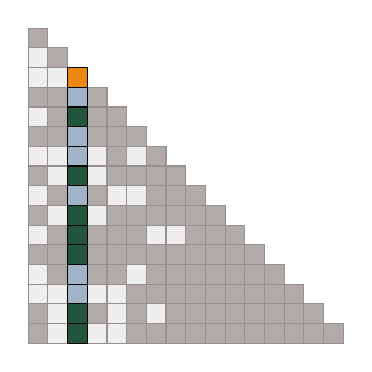
\begin{tikzpicture}[scale=4/16]
  \filldraw[draw=nnzborder, fill=nnzcolor] (0, 0) rectangle (1, -1);
  \filldraw[draw=zeroborder, fill=zerocolor] (0, -1) rectangle (1, -2);
  \filldraw[draw=zeroborder, fill=zerocolor] (0, -2) rectangle (1, -3);
  \filldraw[draw=nnzborder, fill=nnzcolor] (0, -3) rectangle (1, -4);
  \filldraw[draw=zeroborder, fill=zerocolor] (0, -4) rectangle (1, -5);
  \filldraw[draw=nnzborder, fill=nnzcolor] (0, -5) rectangle (1, -6);
  \filldraw[draw=zeroborder, fill=zerocolor] (0, -6) rectangle (1, -7);
  \filldraw[draw=nnzborder, fill=nnzcolor] (0, -7) rectangle (1, -8);
  \filldraw[draw=zeroborder, fill=zerocolor] (0, -8) rectangle (1, -9);
  \filldraw[draw=nnzborder, fill=nnzcolor] (0, -9) rectangle (1, -10);
  \filldraw[draw=zeroborder, fill=zerocolor] (0, -10) rectangle (1, -11);
  \filldraw[draw=nnzborder, fill=nnzcolor] (0, -11) rectangle (1, -12);
  \filldraw[draw=zeroborder, fill=zerocolor] (0, -12) rectangle (1, -13);
  \filldraw[draw=zeroborder, fill=zerocolor] (0, -13) rectangle (1, -14);
  \filldraw[draw=nnzborder, fill=nnzcolor] (0, -14) rectangle (1, -15);
  \filldraw[draw=nnzborder, fill=nnzcolor] (0, -15) rectangle (1, -16);
  \filldraw[draw=nnzborder, fill=nnzcolor] (1, -1) rectangle (2, -2);
  \filldraw[draw=zeroborder, fill=zerocolor] (1, -2) rectangle (2, -3);
  \filldraw[draw=nnzborder, fill=nnzcolor] (1, -3) rectangle (2, -4);
  \filldraw[draw=nnzborder, fill=nnzcolor] (1, -4) rectangle (2, -5);
  \filldraw[draw=nnzborder, fill=nnzcolor] (1, -5) rectangle (2, -6);
  \filldraw[draw=zeroborder, fill=zerocolor] (1, -6) rectangle (2, -7);
  \filldraw[draw=zeroborder, fill=zerocolor] (1, -7) rectangle (2, -8);
  \filldraw[draw=nnzborder, fill=nnzcolor] (1, -8) rectangle (2, -9);
  \filldraw[draw=zeroborder, fill=zerocolor] (1, -9) rectangle (2, -10);
  \filldraw[draw=nnzborder, fill=nnzcolor] (1, -10) rectangle (2, -11);
  \filldraw[draw=nnzborder, fill=nnzcolor] (1, -11) rectangle (2, -12);
  \filldraw[draw=nnzborder, fill=nnzcolor] (1, -12) rectangle (2, -13);
  \filldraw[draw=zeroborder, fill=zerocolor] (1, -13) rectangle (2, -14);
  \filldraw[draw=zeroborder, fill=zerocolor] (1, -14) rectangle (2, -15);
  \filldraw[draw=zeroborder, fill=zerocolor] (1, -15) rectangle (2, -16);
  \filldraw[draw=nnzborder, fill=nnzcolor] (3, -3) rectangle (4, -4);
  \filldraw[draw=nnzborder, fill=nnzcolor] (3, -4) rectangle (4, -5);
  \filldraw[draw=nnzborder, fill=nnzcolor] (3, -5) rectangle (4, -6);
  \filldraw[draw=zeroborder, fill=zerocolor] (3, -6) rectangle (4, -7);
  \filldraw[draw=zeroborder, fill=zerocolor] (3, -7) rectangle (4, -8);
  \filldraw[draw=nnzborder, fill=nnzcolor] (3, -8) rectangle (4, -9);
  \filldraw[draw=zeroborder, fill=zerocolor] (3, -9) rectangle (4, -10);
  \filldraw[draw=nnzborder, fill=nnzcolor] (3, -10) rectangle (4, -11);
  \filldraw[draw=nnzborder, fill=nnzcolor] (3, -11) rectangle (4, -12);
  \filldraw[draw=nnzborder, fill=nnzcolor] (3, -12) rectangle (4, -13);
  \filldraw[draw=zeroborder, fill=zerocolor] (3, -13) rectangle (4, -14);
  \filldraw[draw=nnzborder, fill=nnzcolor] (3, -14) rectangle (4, -15);
  \filldraw[draw=zeroborder, fill=zerocolor] (3, -15) rectangle (4, -16);
  \filldraw[draw=nnzborder, fill=nnzcolor] (4, -4) rectangle (5, -5);
  \filldraw[draw=nnzborder, fill=nnzcolor] (4, -5) rectangle (5, -6);
  \filldraw[draw=nnzborder, fill=nnzcolor] (4, -6) rectangle (5, -7);
  \filldraw[draw=nnzborder, fill=nnzcolor] (4, -7) rectangle (5, -8);
  \filldraw[draw=zeroborder, fill=zerocolor] (4, -8) rectangle (5, -9);
  \filldraw[draw=nnzborder, fill=nnzcolor] (4, -9) rectangle (5, -10);
  \filldraw[draw=nnzborder, fill=nnzcolor] (4, -10) rectangle (5, -11);
  \filldraw[draw=nnzborder, fill=nnzcolor] (4, -11) rectangle (5, -12);
  \filldraw[draw=nnzborder, fill=nnzcolor] (4, -12) rectangle (5, -13);
  \filldraw[draw=zeroborder, fill=zerocolor] (4, -13) rectangle (5, -14);
  \filldraw[draw=zeroborder, fill=zerocolor] (4, -14) rectangle (5, -15);
  \filldraw[draw=zeroborder, fill=zerocolor] (4, -15) rectangle (5, -16);
  \filldraw[draw=nnzborder, fill=nnzcolor] (5, -5) rectangle (6, -6);
  \filldraw[draw=zeroborder, fill=zerocolor] (5, -6) rectangle (6, -7);
  \filldraw[draw=nnzborder, fill=nnzcolor] (5, -7) rectangle (6, -8);
  \filldraw[draw=zeroborder, fill=zerocolor] (5, -8) rectangle (6, -9);
  \filldraw[draw=nnzborder, fill=nnzcolor] (5, -9) rectangle (6, -10);
  \filldraw[draw=nnzborder, fill=nnzcolor] (5, -10) rectangle (6, -11);
  \filldraw[draw=nnzborder, fill=nnzcolor] (5, -11) rectangle (6, -12);
  \filldraw[draw=zeroborder, fill=zerocolor] (5, -12) rectangle (6, -13);
  \filldraw[draw=nnzborder, fill=nnzcolor] (5, -13) rectangle (6, -14);
  \filldraw[draw=nnzborder, fill=nnzcolor] (5, -14) rectangle (6, -15);
  \filldraw[draw=nnzborder, fill=nnzcolor] (5, -15) rectangle (6, -16);
  \filldraw[draw=nnzborder, fill=nnzcolor] (6, -6) rectangle (7, -7);
  \filldraw[draw=nnzborder, fill=nnzcolor] (6, -7) rectangle (7, -8);
  \filldraw[draw=nnzborder, fill=nnzcolor] (6, -8) rectangle (7, -9);
  \filldraw[draw=nnzborder, fill=nnzcolor] (6, -9) rectangle (7, -10);
  \filldraw[draw=zeroborder, fill=zerocolor] (6, -10) rectangle (7, -11);
  \filldraw[draw=nnzborder, fill=nnzcolor] (6, -11) rectangle (7, -12);
  \filldraw[draw=nnzborder, fill=nnzcolor] (6, -12) rectangle (7, -13);
  \filldraw[draw=nnzborder, fill=nnzcolor] (6, -13) rectangle (7, -14);
  \filldraw[draw=zeroborder, fill=zerocolor] (6, -14) rectangle (7, -15);
  \filldraw[draw=nnzborder, fill=nnzcolor] (6, -15) rectangle (7, -16);
  \filldraw[draw=nnzborder, fill=nnzcolor] (7, -7) rectangle (8, -8);
  \filldraw[draw=nnzborder, fill=nnzcolor] (7, -8) rectangle (8, -9);
  \filldraw[draw=nnzborder, fill=nnzcolor] (7, -9) rectangle (8, -10);
  \filldraw[draw=zeroborder, fill=zerocolor] (7, -10) rectangle (8, -11);
  \filldraw[draw=nnzborder, fill=nnzcolor] (7, -11) rectangle (8, -12);
  \filldraw[draw=nnzborder, fill=nnzcolor] (7, -12) rectangle (8, -13);
  \filldraw[draw=nnzborder, fill=nnzcolor] (7, -13) rectangle (8, -14);
  \filldraw[draw=nnzborder, fill=nnzcolor] (7, -14) rectangle (8, -15);
  \filldraw[draw=nnzborder, fill=nnzcolor] (7, -15) rectangle (8, -16);
  \filldraw[draw=nnzborder, fill=nnzcolor] (8, -8) rectangle (9, -9);
  \filldraw[draw=nnzborder, fill=nnzcolor] (8, -9) rectangle (9, -10);
  \filldraw[draw=nnzborder, fill=nnzcolor] (8, -10) rectangle (9, -11);
  \filldraw[draw=nnzborder, fill=nnzcolor] (8, -11) rectangle (9, -12);
  \filldraw[draw=nnzborder, fill=nnzcolor] (8, -12) rectangle (9, -13);
  \filldraw[draw=nnzborder, fill=nnzcolor] (8, -13) rectangle (9, -14);
  \filldraw[draw=nnzborder, fill=nnzcolor] (8, -14) rectangle (9, -15);
  \filldraw[draw=nnzborder, fill=nnzcolor] (8, -15) rectangle (9, -16);
  \filldraw[draw=nnzborder, fill=nnzcolor] (9, -9) rectangle (10, -10);
  \filldraw[draw=nnzborder, fill=nnzcolor] (9, -10) rectangle (10, -11);
  \filldraw[draw=nnzborder, fill=nnzcolor] (9, -11) rectangle (10, -12);
  \filldraw[draw=nnzborder, fill=nnzcolor] (9, -12) rectangle (10, -13);
  \filldraw[draw=nnzborder, fill=nnzcolor] (9, -13) rectangle (10, -14);
  \filldraw[draw=nnzborder, fill=nnzcolor] (9, -14) rectangle (10, -15);
  \filldraw[draw=nnzborder, fill=nnzcolor] (9, -15) rectangle (10, -16);
  \filldraw[draw=nnzborder, fill=nnzcolor] (10, -10) rectangle (11, -11);
  \filldraw[draw=nnzborder, fill=nnzcolor] (10, -11) rectangle (11, -12);
  \filldraw[draw=nnzborder, fill=nnzcolor] (10, -12) rectangle (11, -13);
  \filldraw[draw=nnzborder, fill=nnzcolor] (10, -13) rectangle (11, -14);
  \filldraw[draw=nnzborder, fill=nnzcolor] (10, -14) rectangle (11, -15);
  \filldraw[draw=nnzborder, fill=nnzcolor] (10, -15) rectangle (11, -16);
  \filldraw[draw=nnzborder, fill=nnzcolor] (11, -11) rectangle (12, -12);
  \filldraw[draw=nnzborder, fill=nnzcolor] (11, -12) rectangle (12, -13);
  \filldraw[draw=nnzborder, fill=nnzcolor] (11, -13) rectangle (12, -14);
  \filldraw[draw=nnzborder, fill=nnzcolor] (11, -14) rectangle (12, -15);
  \filldraw[draw=nnzborder, fill=nnzcolor] (11, -15) rectangle (12, -16);
  \filldraw[draw=nnzborder, fill=nnzcolor] (12, -12) rectangle (13, -13);
  \filldraw[draw=nnzborder, fill=nnzcolor] (12, -13) rectangle (13, -14);
  \filldraw[draw=nnzborder, fill=nnzcolor] (12, -14) rectangle (13, -15);
  \filldraw[draw=nnzborder, fill=nnzcolor] (12, -15) rectangle (13, -16);
  \filldraw[draw=nnzborder, fill=nnzcolor] (13, -13) rectangle (14, -14);
  \filldraw[draw=nnzborder, fill=nnzcolor] (13, -14) rectangle (14, -15);
  \filldraw[draw=nnzborder, fill=nnzcolor] (13, -15) rectangle (14, -16);
  \filldraw[draw=nnzborder, fill=nnzcolor] (14, -14) rectangle (15, -15);
  \filldraw[draw=nnzborder, fill=nnzcolor] (14, -15) rectangle (15, -16);
  \filldraw[draw=nnzborder, fill=nnzcolor] (15, -15) rectangle (16, -16);
  \filldraw[draw=colborder, fill=targetcolor] (2, -2) rectangle (3, -3);
  \filldraw[draw=colborder, fill=candcolor] (2, -3) rectangle (3, -4);
  \filldraw[draw=colborder, fill=selcolor] (2, -4) rectangle (3, -5);
  \filldraw[draw=colborder, fill=candcolor] (2, -5) rectangle (3, -6);
  \filldraw[draw=colborder, fill=candcolor] (2, -6) rectangle (3, -7);
  \filldraw[draw=colborder, fill=selcolor] (2, -7) rectangle (3, -8);
  \filldraw[draw=colborder, fill=candcolor] (2, -8) rectangle (3, -9);
  \filldraw[draw=colborder, fill=selcolor] (2, -9) rectangle (3, -10);
  \filldraw[draw=colborder, fill=selcolor] (2, -10) rectangle (3, -11);
  \filldraw[draw=colborder, fill=selcolor] (2, -11) rectangle (3, -12);
  \filldraw[draw=colborder, fill=candcolor] (2, -12) rectangle (3, -13);
  \filldraw[draw=colborder, fill=candcolor] (2, -13) rectangle (3, -14);
  \filldraw[draw=colborder, fill=selcolor] (2, -14) rectangle (3, -15);
  \filldraw[draw=colborder, fill=selcolor] (2, -15) rectangle (3, -16);
\end{tikzpicture}
%
    \qquad
    \begin{tikzpicture}[baseline]
  \begin{axis}[
    % calculated from Cholesky factor, exactly 16 cm x 16 cm
    width={4cm},
    height={4cm},
    axis lines={none},
    % force axis box to have exactly the right dimensions, ignoring labels
    scale only axis=true,
  ]
  % consistent size bounding box
  \draw [white, line width=0] (-0.1, -0.1) -- (-0.1,  1.1);
  \draw [white, line width=0] ( 1.1, -0.1) -- ( 1.1,  1.1);
  \draw [white, line width=0] (-0.1, -0.1) -- (-1.1, -0.1);
  \draw [white, line width=0] (-0.1,  1.1) -- (-1.1,  1.1);
  \draw [seagreen!15, fill, radius=0.5361056327819824] (0.030346007662471197, 0.7069650956556235) circle;
  \draw [seagreen, radius=0.5361056327819824] (0.030346007662471197, 0.7069650956556235) circle;
  \draw [orange!25, fill, radius=0.2680528163909912] (0.030346007662471197, 0.7069650956556235) circle;
  \draw [orange, radius=0.2680528163909912] (0.030346007662471197, 0.7069650956556235) circle;
  \addplot [only marks, mark size=1, silver]    table
    {figures/points_knn/all_points.csv};
  \addplot [only marks, mark size=2, lightblue] table
    {figures/points_knn/candidates_08.csv};
  \addplot [only marks, mark size=4, seagreen]  table
    {figures/points_knn/selected_08.csv};
  \addplot [only marks, mark size=4, orange]    table
    {figures/points_knn/target_08.csv};
  \end{axis}
\end{tikzpicture}

  \end{figure}
}
\only<9>{
  \begin{figure}
    \centering
    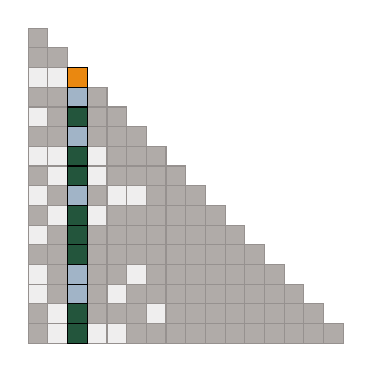
\begin{tikzpicture}[scale=4/16]
  \filldraw[draw=nnzborder, fill=nnzcolor] (0, 0) rectangle (1, -1);
  \filldraw[draw=nnzborder, fill=nnzcolor] (0, -1) rectangle (1, -2);
  \filldraw[draw=zeroborder, fill=zerocolor] (0, -2) rectangle (1, -3);
  \filldraw[draw=nnzborder, fill=nnzcolor] (0, -3) rectangle (1, -4);
  \filldraw[draw=zeroborder, fill=zerocolor] (0, -4) rectangle (1, -5);
  \filldraw[draw=nnzborder, fill=nnzcolor] (0, -5) rectangle (1, -6);
  \filldraw[draw=zeroborder, fill=zerocolor] (0, -6) rectangle (1, -7);
  \filldraw[draw=nnzborder, fill=nnzcolor] (0, -7) rectangle (1, -8);
  \filldraw[draw=zeroborder, fill=zerocolor] (0, -8) rectangle (1, -9);
  \filldraw[draw=nnzborder, fill=nnzcolor] (0, -9) rectangle (1, -10);
  \filldraw[draw=zeroborder, fill=zerocolor] (0, -10) rectangle (1, -11);
  \filldraw[draw=nnzborder, fill=nnzcolor] (0, -11) rectangle (1, -12);
  \filldraw[draw=zeroborder, fill=zerocolor] (0, -12) rectangle (1, -13);
  \filldraw[draw=zeroborder, fill=zerocolor] (0, -13) rectangle (1, -14);
  \filldraw[draw=nnzborder, fill=nnzcolor] (0, -14) rectangle (1, -15);
  \filldraw[draw=nnzborder, fill=nnzcolor] (0, -15) rectangle (1, -16);
  \filldraw[draw=nnzborder, fill=nnzcolor] (1, -1) rectangle (2, -2);
  \filldraw[draw=zeroborder, fill=zerocolor] (1, -2) rectangle (2, -3);
  \filldraw[draw=nnzborder, fill=nnzcolor] (1, -3) rectangle (2, -4);
  \filldraw[draw=nnzborder, fill=nnzcolor] (1, -4) rectangle (2, -5);
  \filldraw[draw=nnzborder, fill=nnzcolor] (1, -5) rectangle (2, -6);
  \filldraw[draw=zeroborder, fill=zerocolor] (1, -6) rectangle (2, -7);
  \filldraw[draw=zeroborder, fill=zerocolor] (1, -7) rectangle (2, -8);
  \filldraw[draw=nnzborder, fill=nnzcolor] (1, -8) rectangle (2, -9);
  \filldraw[draw=zeroborder, fill=zerocolor] (1, -9) rectangle (2, -10);
  \filldraw[draw=nnzborder, fill=nnzcolor] (1, -10) rectangle (2, -11);
  \filldraw[draw=nnzborder, fill=nnzcolor] (1, -11) rectangle (2, -12);
  \filldraw[draw=nnzborder, fill=nnzcolor] (1, -12) rectangle (2, -13);
  \filldraw[draw=nnzborder, fill=nnzcolor] (1, -13) rectangle (2, -14);
  \filldraw[draw=zeroborder, fill=zerocolor] (1, -14) rectangle (2, -15);
  \filldraw[draw=zeroborder, fill=zerocolor] (1, -15) rectangle (2, -16);
  \filldraw[draw=nnzborder, fill=nnzcolor] (3, -3) rectangle (4, -4);
  \filldraw[draw=nnzborder, fill=nnzcolor] (3, -4) rectangle (4, -5);
  \filldraw[draw=nnzborder, fill=nnzcolor] (3, -5) rectangle (4, -6);
  \filldraw[draw=zeroborder, fill=zerocolor] (3, -6) rectangle (4, -7);
  \filldraw[draw=zeroborder, fill=zerocolor] (3, -7) rectangle (4, -8);
  \filldraw[draw=nnzborder, fill=nnzcolor] (3, -8) rectangle (4, -9);
  \filldraw[draw=zeroborder, fill=zerocolor] (3, -9) rectangle (4, -10);
  \filldraw[draw=nnzborder, fill=nnzcolor] (3, -10) rectangle (4, -11);
  \filldraw[draw=nnzborder, fill=nnzcolor] (3, -11) rectangle (4, -12);
  \filldraw[draw=nnzborder, fill=nnzcolor] (3, -12) rectangle (4, -13);
  \filldraw[draw=nnzborder, fill=nnzcolor] (3, -13) rectangle (4, -14);
  \filldraw[draw=nnzborder, fill=nnzcolor] (3, -14) rectangle (4, -15);
  \filldraw[draw=zeroborder, fill=zerocolor] (3, -15) rectangle (4, -16);
  \filldraw[draw=nnzborder, fill=nnzcolor] (4, -4) rectangle (5, -5);
  \filldraw[draw=nnzborder, fill=nnzcolor] (4, -5) rectangle (5, -6);
  \filldraw[draw=nnzborder, fill=nnzcolor] (4, -6) rectangle (5, -7);
  \filldraw[draw=nnzborder, fill=nnzcolor] (4, -7) rectangle (5, -8);
  \filldraw[draw=zeroborder, fill=zerocolor] (4, -8) rectangle (5, -9);
  \filldraw[draw=nnzborder, fill=nnzcolor] (4, -9) rectangle (5, -10);
  \filldraw[draw=nnzborder, fill=nnzcolor] (4, -10) rectangle (5, -11);
  \filldraw[draw=nnzborder, fill=nnzcolor] (4, -11) rectangle (5, -12);
  \filldraw[draw=nnzborder, fill=nnzcolor] (4, -12) rectangle (5, -13);
  \filldraw[draw=zeroborder, fill=zerocolor] (4, -13) rectangle (5, -14);
  \filldraw[draw=nnzborder, fill=nnzcolor] (4, -14) rectangle (5, -15);
  \filldraw[draw=zeroborder, fill=zerocolor] (4, -15) rectangle (5, -16);
  \filldraw[draw=nnzborder, fill=nnzcolor] (5, -5) rectangle (6, -6);
  \filldraw[draw=nnzborder, fill=nnzcolor] (5, -6) rectangle (6, -7);
  \filldraw[draw=nnzborder, fill=nnzcolor] (5, -7) rectangle (6, -8);
  \filldraw[draw=zeroborder, fill=zerocolor] (5, -8) rectangle (6, -9);
  \filldraw[draw=nnzborder, fill=nnzcolor] (5, -9) rectangle (6, -10);
  \filldraw[draw=nnzborder, fill=nnzcolor] (5, -10) rectangle (6, -11);
  \filldraw[draw=nnzborder, fill=nnzcolor] (5, -11) rectangle (6, -12);
  \filldraw[draw=zeroborder, fill=zerocolor] (5, -12) rectangle (6, -13);
  \filldraw[draw=nnzborder, fill=nnzcolor] (5, -13) rectangle (6, -14);
  \filldraw[draw=nnzborder, fill=nnzcolor] (5, -14) rectangle (6, -15);
  \filldraw[draw=nnzborder, fill=nnzcolor] (5, -15) rectangle (6, -16);
  \filldraw[draw=nnzborder, fill=nnzcolor] (6, -6) rectangle (7, -7);
  \filldraw[draw=nnzborder, fill=nnzcolor] (6, -7) rectangle (7, -8);
  \filldraw[draw=nnzborder, fill=nnzcolor] (6, -8) rectangle (7, -9);
  \filldraw[draw=nnzborder, fill=nnzcolor] (6, -9) rectangle (7, -10);
  \filldraw[draw=nnzborder, fill=nnzcolor] (6, -10) rectangle (7, -11);
  \filldraw[draw=nnzborder, fill=nnzcolor] (6, -11) rectangle (7, -12);
  \filldraw[draw=nnzborder, fill=nnzcolor] (6, -12) rectangle (7, -13);
  \filldraw[draw=nnzborder, fill=nnzcolor] (6, -13) rectangle (7, -14);
  \filldraw[draw=zeroborder, fill=zerocolor] (6, -14) rectangle (7, -15);
  \filldraw[draw=nnzborder, fill=nnzcolor] (6, -15) rectangle (7, -16);
  \filldraw[draw=nnzborder, fill=nnzcolor] (7, -7) rectangle (8, -8);
  \filldraw[draw=nnzborder, fill=nnzcolor] (7, -8) rectangle (8, -9);
  \filldraw[draw=nnzborder, fill=nnzcolor] (7, -9) rectangle (8, -10);
  \filldraw[draw=nnzborder, fill=nnzcolor] (7, -10) rectangle (8, -11);
  \filldraw[draw=nnzborder, fill=nnzcolor] (7, -11) rectangle (8, -12);
  \filldraw[draw=nnzborder, fill=nnzcolor] (7, -12) rectangle (8, -13);
  \filldraw[draw=nnzborder, fill=nnzcolor] (7, -13) rectangle (8, -14);
  \filldraw[draw=nnzborder, fill=nnzcolor] (7, -14) rectangle (8, -15);
  \filldraw[draw=nnzborder, fill=nnzcolor] (7, -15) rectangle (8, -16);
  \filldraw[draw=nnzborder, fill=nnzcolor] (8, -8) rectangle (9, -9);
  \filldraw[draw=nnzborder, fill=nnzcolor] (8, -9) rectangle (9, -10);
  \filldraw[draw=nnzborder, fill=nnzcolor] (8, -10) rectangle (9, -11);
  \filldraw[draw=nnzborder, fill=nnzcolor] (8, -11) rectangle (9, -12);
  \filldraw[draw=nnzborder, fill=nnzcolor] (8, -12) rectangle (9, -13);
  \filldraw[draw=nnzborder, fill=nnzcolor] (8, -13) rectangle (9, -14);
  \filldraw[draw=nnzborder, fill=nnzcolor] (8, -14) rectangle (9, -15);
  \filldraw[draw=nnzborder, fill=nnzcolor] (8, -15) rectangle (9, -16);
  \filldraw[draw=nnzborder, fill=nnzcolor] (9, -9) rectangle (10, -10);
  \filldraw[draw=nnzborder, fill=nnzcolor] (9, -10) rectangle (10, -11);
  \filldraw[draw=nnzborder, fill=nnzcolor] (9, -11) rectangle (10, -12);
  \filldraw[draw=nnzborder, fill=nnzcolor] (9, -12) rectangle (10, -13);
  \filldraw[draw=nnzborder, fill=nnzcolor] (9, -13) rectangle (10, -14);
  \filldraw[draw=nnzborder, fill=nnzcolor] (9, -14) rectangle (10, -15);
  \filldraw[draw=nnzborder, fill=nnzcolor] (9, -15) rectangle (10, -16);
  \filldraw[draw=nnzborder, fill=nnzcolor] (10, -10) rectangle (11, -11);
  \filldraw[draw=nnzborder, fill=nnzcolor] (10, -11) rectangle (11, -12);
  \filldraw[draw=nnzborder, fill=nnzcolor] (10, -12) rectangle (11, -13);
  \filldraw[draw=nnzborder, fill=nnzcolor] (10, -13) rectangle (11, -14);
  \filldraw[draw=nnzborder, fill=nnzcolor] (10, -14) rectangle (11, -15);
  \filldraw[draw=nnzborder, fill=nnzcolor] (10, -15) rectangle (11, -16);
  \filldraw[draw=nnzborder, fill=nnzcolor] (11, -11) rectangle (12, -12);
  \filldraw[draw=nnzborder, fill=nnzcolor] (11, -12) rectangle (12, -13);
  \filldraw[draw=nnzborder, fill=nnzcolor] (11, -13) rectangle (12, -14);
  \filldraw[draw=nnzborder, fill=nnzcolor] (11, -14) rectangle (12, -15);
  \filldraw[draw=nnzborder, fill=nnzcolor] (11, -15) rectangle (12, -16);
  \filldraw[draw=nnzborder, fill=nnzcolor] (12, -12) rectangle (13, -13);
  \filldraw[draw=nnzborder, fill=nnzcolor] (12, -13) rectangle (13, -14);
  \filldraw[draw=nnzborder, fill=nnzcolor] (12, -14) rectangle (13, -15);
  \filldraw[draw=nnzborder, fill=nnzcolor] (12, -15) rectangle (13, -16);
  \filldraw[draw=nnzborder, fill=nnzcolor] (13, -13) rectangle (14, -14);
  \filldraw[draw=nnzborder, fill=nnzcolor] (13, -14) rectangle (14, -15);
  \filldraw[draw=nnzborder, fill=nnzcolor] (13, -15) rectangle (14, -16);
  \filldraw[draw=nnzborder, fill=nnzcolor] (14, -14) rectangle (15, -15);
  \filldraw[draw=nnzborder, fill=nnzcolor] (14, -15) rectangle (15, -16);
  \filldraw[draw=nnzborder, fill=nnzcolor] (15, -15) rectangle (16, -16);
  \filldraw[draw=colborder, fill=targetcolor] (2, -2) rectangle (3, -3);
  \filldraw[draw=colborder, fill=candcolor] (2, -3) rectangle (3, -4);
  \filldraw[draw=colborder, fill=selcolor] (2, -4) rectangle (3, -5);
  \filldraw[draw=colborder, fill=candcolor] (2, -5) rectangle (3, -6);
  \filldraw[draw=colborder, fill=selcolor] (2, -6) rectangle (3, -7);
  \filldraw[draw=colborder, fill=selcolor] (2, -7) rectangle (3, -8);
  \filldraw[draw=colborder, fill=candcolor] (2, -8) rectangle (3, -9);
  \filldraw[draw=colborder, fill=selcolor] (2, -9) rectangle (3, -10);
  \filldraw[draw=colborder, fill=selcolor] (2, -10) rectangle (3, -11);
  \filldraw[draw=colborder, fill=selcolor] (2, -11) rectangle (3, -12);
  \filldraw[draw=colborder, fill=candcolor] (2, -12) rectangle (3, -13);
  \filldraw[draw=colborder, fill=candcolor] (2, -13) rectangle (3, -14);
  \filldraw[draw=colborder, fill=selcolor] (2, -14) rectangle (3, -15);
  \filldraw[draw=colborder, fill=selcolor] (2, -15) rectangle (3, -16);
\end{tikzpicture}
%
    \qquad
    \begin{tikzpicture}[baseline]
  \begin{axis}[
    % calculated from Cholesky factor, exactly 16 cm x 16 cm
    width={4cm},
    height={4cm},
    axis lines={none},
    % force axis box to have exactly the right dimensions, ignoring labels
    scale only axis=true,
  ]
  % consistent size bounding box
  \draw [white, line width=0] (-0.1, -0.1) -- (-0.1,  1.1);
  \draw [white, line width=0] ( 1.1, -0.1) -- ( 1.1,  1.1);
  \draw [white, line width=0] (-0.1, -0.1) -- (-1.1, -0.1);
  \draw [white, line width=0] (-0.1,  1.1) -- (-1.1,  1.1);
  \draw [seagreen!15, fill, radius=0.452634334564209] (0.29840122301687566, 0.3139860020343368) circle;
  \draw [seagreen, radius=0.452634334564209] (0.29840122301687566, 0.3139860020343368) circle;
  \draw [orange!25, fill, radius=0.2263171672821045] (0.29840122301687566, 0.3139860020343368) circle;
  \draw [orange, radius=0.2263171672821045] (0.29840122301687566, 0.3139860020343368) circle;
  \addplot [only marks, mark size=1, silver]    table
    {figures/points_knn/all_points.csv};
  \addplot [only marks, mark size=2, lightblue] table
    {figures/points_knn/candidates_09.csv};
  \addplot [only marks, mark size=4, seagreen]  table
    {figures/points_knn/selected_09.csv};
  \addplot [only marks, mark size=4, orange]    table
    {figures/points_knn/target_09.csv};
  \end{axis}
\end{tikzpicture}

  \end{figure}
}
\only<10>{
  \begin{figure}
    \centering
    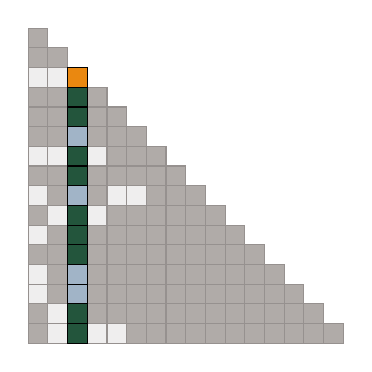
\begin{tikzpicture}[scale=4/16]
  \filldraw[draw=nnzborder, fill=nnzcolor] (0, 0) rectangle (1, -1);
  \filldraw[draw=nnzborder, fill=nnzcolor] (0, -1) rectangle (1, -2);
  \filldraw[draw=zeroborder, fill=zerocolor] (0, -2) rectangle (1, -3);
  \filldraw[draw=nnzborder, fill=nnzcolor] (0, -3) rectangle (1, -4);
  \filldraw[draw=nnzborder, fill=nnzcolor] (0, -4) rectangle (1, -5);
  \filldraw[draw=nnzborder, fill=nnzcolor] (0, -5) rectangle (1, -6);
  \filldraw[draw=zeroborder, fill=zerocolor] (0, -6) rectangle (1, -7);
  \filldraw[draw=nnzborder, fill=nnzcolor] (0, -7) rectangle (1, -8);
  \filldraw[draw=zeroborder, fill=zerocolor] (0, -8) rectangle (1, -9);
  \filldraw[draw=nnzborder, fill=nnzcolor] (0, -9) rectangle (1, -10);
  \filldraw[draw=zeroborder, fill=zerocolor] (0, -10) rectangle (1, -11);
  \filldraw[draw=nnzborder, fill=nnzcolor] (0, -11) rectangle (1, -12);
  \filldraw[draw=zeroborder, fill=zerocolor] (0, -12) rectangle (1, -13);
  \filldraw[draw=zeroborder, fill=zerocolor] (0, -13) rectangle (1, -14);
  \filldraw[draw=nnzborder, fill=nnzcolor] (0, -14) rectangle (1, -15);
  \filldraw[draw=nnzborder, fill=nnzcolor] (0, -15) rectangle (1, -16);
  \filldraw[draw=nnzborder, fill=nnzcolor] (1, -1) rectangle (2, -2);
  \filldraw[draw=zeroborder, fill=zerocolor] (1, -2) rectangle (2, -3);
  \filldraw[draw=nnzborder, fill=nnzcolor] (1, -3) rectangle (2, -4);
  \filldraw[draw=nnzborder, fill=nnzcolor] (1, -4) rectangle (2, -5);
  \filldraw[draw=nnzborder, fill=nnzcolor] (1, -5) rectangle (2, -6);
  \filldraw[draw=zeroborder, fill=zerocolor] (1, -6) rectangle (2, -7);
  \filldraw[draw=nnzborder, fill=nnzcolor] (1, -7) rectangle (2, -8);
  \filldraw[draw=nnzborder, fill=nnzcolor] (1, -8) rectangle (2, -9);
  \filldraw[draw=zeroborder, fill=zerocolor] (1, -9) rectangle (2, -10);
  \filldraw[draw=nnzborder, fill=nnzcolor] (1, -10) rectangle (2, -11);
  \filldraw[draw=nnzborder, fill=nnzcolor] (1, -11) rectangle (2, -12);
  \filldraw[draw=nnzborder, fill=nnzcolor] (1, -12) rectangle (2, -13);
  \filldraw[draw=nnzborder, fill=nnzcolor] (1, -13) rectangle (2, -14);
  \filldraw[draw=zeroborder, fill=zerocolor] (1, -14) rectangle (2, -15);
  \filldraw[draw=zeroborder, fill=zerocolor] (1, -15) rectangle (2, -16);
  \filldraw[draw=nnzborder, fill=nnzcolor] (3, -3) rectangle (4, -4);
  \filldraw[draw=nnzborder, fill=nnzcolor] (3, -4) rectangle (4, -5);
  \filldraw[draw=nnzborder, fill=nnzcolor] (3, -5) rectangle (4, -6);
  \filldraw[draw=zeroborder, fill=zerocolor] (3, -6) rectangle (4, -7);
  \filldraw[draw=nnzborder, fill=nnzcolor] (3, -7) rectangle (4, -8);
  \filldraw[draw=nnzborder, fill=nnzcolor] (3, -8) rectangle (4, -9);
  \filldraw[draw=zeroborder, fill=zerocolor] (3, -9) rectangle (4, -10);
  \filldraw[draw=nnzborder, fill=nnzcolor] (3, -10) rectangle (4, -11);
  \filldraw[draw=nnzborder, fill=nnzcolor] (3, -11) rectangle (4, -12);
  \filldraw[draw=nnzborder, fill=nnzcolor] (3, -12) rectangle (4, -13);
  \filldraw[draw=nnzborder, fill=nnzcolor] (3, -13) rectangle (4, -14);
  \filldraw[draw=nnzborder, fill=nnzcolor] (3, -14) rectangle (4, -15);
  \filldraw[draw=zeroborder, fill=zerocolor] (3, -15) rectangle (4, -16);
  \filldraw[draw=nnzborder, fill=nnzcolor] (4, -4) rectangle (5, -5);
  \filldraw[draw=nnzborder, fill=nnzcolor] (4, -5) rectangle (5, -6);
  \filldraw[draw=nnzborder, fill=nnzcolor] (4, -6) rectangle (5, -7);
  \filldraw[draw=nnzborder, fill=nnzcolor] (4, -7) rectangle (5, -8);
  \filldraw[draw=zeroborder, fill=zerocolor] (4, -8) rectangle (5, -9);
  \filldraw[draw=nnzborder, fill=nnzcolor] (4, -9) rectangle (5, -10);
  \filldraw[draw=nnzborder, fill=nnzcolor] (4, -10) rectangle (5, -11);
  \filldraw[draw=nnzborder, fill=nnzcolor] (4, -11) rectangle (5, -12);
  \filldraw[draw=nnzborder, fill=nnzcolor] (4, -12) rectangle (5, -13);
  \filldraw[draw=nnzborder, fill=nnzcolor] (4, -13) rectangle (5, -14);
  \filldraw[draw=nnzborder, fill=nnzcolor] (4, -14) rectangle (5, -15);
  \filldraw[draw=zeroborder, fill=zerocolor] (4, -15) rectangle (5, -16);
  \filldraw[draw=nnzborder, fill=nnzcolor] (5, -5) rectangle (6, -6);
  \filldraw[draw=nnzborder, fill=nnzcolor] (5, -6) rectangle (6, -7);
  \filldraw[draw=nnzborder, fill=nnzcolor] (5, -7) rectangle (6, -8);
  \filldraw[draw=zeroborder, fill=zerocolor] (5, -8) rectangle (6, -9);
  \filldraw[draw=nnzborder, fill=nnzcolor] (5, -9) rectangle (6, -10);
  \filldraw[draw=nnzborder, fill=nnzcolor] (5, -10) rectangle (6, -11);
  \filldraw[draw=nnzborder, fill=nnzcolor] (5, -11) rectangle (6, -12);
  \filldraw[draw=nnzborder, fill=nnzcolor] (5, -12) rectangle (6, -13);
  \filldraw[draw=nnzborder, fill=nnzcolor] (5, -13) rectangle (6, -14);
  \filldraw[draw=nnzborder, fill=nnzcolor] (5, -14) rectangle (6, -15);
  \filldraw[draw=nnzborder, fill=nnzcolor] (5, -15) rectangle (6, -16);
  \filldraw[draw=nnzborder, fill=nnzcolor] (6, -6) rectangle (7, -7);
  \filldraw[draw=nnzborder, fill=nnzcolor] (6, -7) rectangle (7, -8);
  \filldraw[draw=nnzborder, fill=nnzcolor] (6, -8) rectangle (7, -9);
  \filldraw[draw=nnzborder, fill=nnzcolor] (6, -9) rectangle (7, -10);
  \filldraw[draw=nnzborder, fill=nnzcolor] (6, -10) rectangle (7, -11);
  \filldraw[draw=nnzborder, fill=nnzcolor] (6, -11) rectangle (7, -12);
  \filldraw[draw=nnzborder, fill=nnzcolor] (6, -12) rectangle (7, -13);
  \filldraw[draw=nnzborder, fill=nnzcolor] (6, -13) rectangle (7, -14);
  \filldraw[draw=nnzborder, fill=nnzcolor] (6, -14) rectangle (7, -15);
  \filldraw[draw=nnzborder, fill=nnzcolor] (6, -15) rectangle (7, -16);
  \filldraw[draw=nnzborder, fill=nnzcolor] (7, -7) rectangle (8, -8);
  \filldraw[draw=nnzborder, fill=nnzcolor] (7, -8) rectangle (8, -9);
  \filldraw[draw=nnzborder, fill=nnzcolor] (7, -9) rectangle (8, -10);
  \filldraw[draw=nnzborder, fill=nnzcolor] (7, -10) rectangle (8, -11);
  \filldraw[draw=nnzborder, fill=nnzcolor] (7, -11) rectangle (8, -12);
  \filldraw[draw=nnzborder, fill=nnzcolor] (7, -12) rectangle (8, -13);
  \filldraw[draw=nnzborder, fill=nnzcolor] (7, -13) rectangle (8, -14);
  \filldraw[draw=nnzborder, fill=nnzcolor] (7, -14) rectangle (8, -15);
  \filldraw[draw=nnzborder, fill=nnzcolor] (7, -15) rectangle (8, -16);
  \filldraw[draw=nnzborder, fill=nnzcolor] (8, -8) rectangle (9, -9);
  \filldraw[draw=nnzborder, fill=nnzcolor] (8, -9) rectangle (9, -10);
  \filldraw[draw=nnzborder, fill=nnzcolor] (8, -10) rectangle (9, -11);
  \filldraw[draw=nnzborder, fill=nnzcolor] (8, -11) rectangle (9, -12);
  \filldraw[draw=nnzborder, fill=nnzcolor] (8, -12) rectangle (9, -13);
  \filldraw[draw=nnzborder, fill=nnzcolor] (8, -13) rectangle (9, -14);
  \filldraw[draw=nnzborder, fill=nnzcolor] (8, -14) rectangle (9, -15);
  \filldraw[draw=nnzborder, fill=nnzcolor] (8, -15) rectangle (9, -16);
  \filldraw[draw=nnzborder, fill=nnzcolor] (9, -9) rectangle (10, -10);
  \filldraw[draw=nnzborder, fill=nnzcolor] (9, -10) rectangle (10, -11);
  \filldraw[draw=nnzborder, fill=nnzcolor] (9, -11) rectangle (10, -12);
  \filldraw[draw=nnzborder, fill=nnzcolor] (9, -12) rectangle (10, -13);
  \filldraw[draw=nnzborder, fill=nnzcolor] (9, -13) rectangle (10, -14);
  \filldraw[draw=nnzborder, fill=nnzcolor] (9, -14) rectangle (10, -15);
  \filldraw[draw=nnzborder, fill=nnzcolor] (9, -15) rectangle (10, -16);
  \filldraw[draw=nnzborder, fill=nnzcolor] (10, -10) rectangle (11, -11);
  \filldraw[draw=nnzborder, fill=nnzcolor] (10, -11) rectangle (11, -12);
  \filldraw[draw=nnzborder, fill=nnzcolor] (10, -12) rectangle (11, -13);
  \filldraw[draw=nnzborder, fill=nnzcolor] (10, -13) rectangle (11, -14);
  \filldraw[draw=nnzborder, fill=nnzcolor] (10, -14) rectangle (11, -15);
  \filldraw[draw=nnzborder, fill=nnzcolor] (10, -15) rectangle (11, -16);
  \filldraw[draw=nnzborder, fill=nnzcolor] (11, -11) rectangle (12, -12);
  \filldraw[draw=nnzborder, fill=nnzcolor] (11, -12) rectangle (12, -13);
  \filldraw[draw=nnzborder, fill=nnzcolor] (11, -13) rectangle (12, -14);
  \filldraw[draw=nnzborder, fill=nnzcolor] (11, -14) rectangle (12, -15);
  \filldraw[draw=nnzborder, fill=nnzcolor] (11, -15) rectangle (12, -16);
  \filldraw[draw=nnzborder, fill=nnzcolor] (12, -12) rectangle (13, -13);
  \filldraw[draw=nnzborder, fill=nnzcolor] (12, -13) rectangle (13, -14);
  \filldraw[draw=nnzborder, fill=nnzcolor] (12, -14) rectangle (13, -15);
  \filldraw[draw=nnzborder, fill=nnzcolor] (12, -15) rectangle (13, -16);
  \filldraw[draw=nnzborder, fill=nnzcolor] (13, -13) rectangle (14, -14);
  \filldraw[draw=nnzborder, fill=nnzcolor] (13, -14) rectangle (14, -15);
  \filldraw[draw=nnzborder, fill=nnzcolor] (13, -15) rectangle (14, -16);
  \filldraw[draw=nnzborder, fill=nnzcolor] (14, -14) rectangle (15, -15);
  \filldraw[draw=nnzborder, fill=nnzcolor] (14, -15) rectangle (15, -16);
  \filldraw[draw=nnzborder, fill=nnzcolor] (15, -15) rectangle (16, -16);
  \filldraw[draw=colborder, fill=targetcolor] (2, -2) rectangle (3, -3);
  \filldraw[draw=colborder, fill=selcolor] (2, -3) rectangle (3, -4);
  \filldraw[draw=colborder, fill=selcolor] (2, -4) rectangle (3, -5);
  \filldraw[draw=colborder, fill=candcolor] (2, -5) rectangle (3, -6);
  \filldraw[draw=colborder, fill=selcolor] (2, -6) rectangle (3, -7);
  \filldraw[draw=colborder, fill=selcolor] (2, -7) rectangle (3, -8);
  \filldraw[draw=colborder, fill=candcolor] (2, -8) rectangle (3, -9);
  \filldraw[draw=colborder, fill=selcolor] (2, -9) rectangle (3, -10);
  \filldraw[draw=colborder, fill=selcolor] (2, -10) rectangle (3, -11);
  \filldraw[draw=colborder, fill=selcolor] (2, -11) rectangle (3, -12);
  \filldraw[draw=colborder, fill=candcolor] (2, -12) rectangle (3, -13);
  \filldraw[draw=colborder, fill=candcolor] (2, -13) rectangle (3, -14);
  \filldraw[draw=colborder, fill=selcolor] (2, -14) rectangle (3, -15);
  \filldraw[draw=colborder, fill=selcolor] (2, -15) rectangle (3, -16);
\end{tikzpicture}
%
    \qquad
    \begin{tikzpicture}[baseline]
  \begin{axis}[
    % calculated from Cholesky factor, exactly 16 cm x 16 cm
    width={4cm},
    height={4cm},
    axis lines={none},
    % force axis box to have exactly the right dimensions, ignoring labels
    scale only axis=true,
  ]
  % consistent size bounding box
  \draw [white, line width=0] (-0.1, -0.1) -- (-0.1,  1.1);
  \draw [white, line width=0] ( 1.1, -0.1) -- ( 1.1,  1.1);
  \draw [white, line width=0] (-0.1, -0.1) -- (-1.1, -0.1);
  \draw [white, line width=0] (-0.1,  1.1) -- (-1.1,  1.1);
  \draw [seagreen!15, fill, radius=0.39299893379211426] (0.09412864224039919, 0.4331269402364738) circle;
  \draw [seagreen, radius=0.39299893379211426] (0.09412864224039919, 0.4331269402364738) circle;
  \draw [orange!25, fill, radius=0.19649946689605713] (0.09412864224039919, 0.4331269402364738) circle;
  \draw [orange, radius=0.19649946689605713] (0.09412864224039919, 0.4331269402364738) circle;
  \addplot [only marks, mark size=1, silver]    table
    {figures/points_knn/all_points.csv};
  \addplot [only marks, mark size=2, lightblue] table
    {figures/points_knn/candidates_10.csv};
  \addplot [only marks, mark size=4, seagreen]  table
    {figures/points_knn/selected_10.csv};
  \addplot [only marks, mark size=4, orange]    table
    {figures/points_knn/target_10.csv};
  \end{axis}
\end{tikzpicture}

  \end{figure}
}
\only<11>{
  \begin{figure}
    \centering
    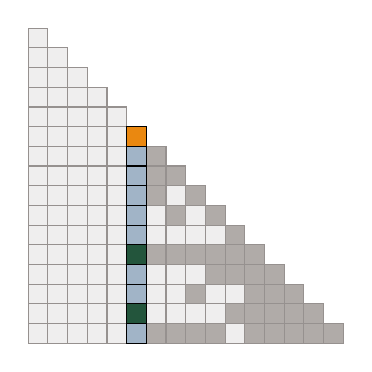
\begin{tikzpicture}[scale=4/16]
  \filldraw[draw=zeroborder, fill=zerocolor] (0, 0) rectangle (1, -1);
  \filldraw[draw=zeroborder, fill=zerocolor] (0, -1) rectangle (1, -2);
  \filldraw[draw=zeroborder, fill=zerocolor] (0, -2) rectangle (1, -3);
  \filldraw[draw=zeroborder, fill=zerocolor] (0, -3) rectangle (1, -4);
  \filldraw[draw=zeroborder, fill=zerocolor] (0, -4) rectangle (1, -5);
  \filldraw[draw=zeroborder, fill=zerocolor] (0, -5) rectangle (1, -6);
  \filldraw[draw=zeroborder, fill=zerocolor] (0, -6) rectangle (1, -7);
  \filldraw[draw=zeroborder, fill=zerocolor] (0, -7) rectangle (1, -8);
  \filldraw[draw=zeroborder, fill=zerocolor] (0, -8) rectangle (1, -9);
  \filldraw[draw=zeroborder, fill=zerocolor] (0, -9) rectangle (1, -10);
  \filldraw[draw=zeroborder, fill=zerocolor] (0, -10) rectangle (1, -11);
  \filldraw[draw=zeroborder, fill=zerocolor] (0, -11) rectangle (1, -12);
  \filldraw[draw=zeroborder, fill=zerocolor] (0, -12) rectangle (1, -13);
  \filldraw[draw=zeroborder, fill=zerocolor] (0, -13) rectangle (1, -14);
  \filldraw[draw=zeroborder, fill=zerocolor] (0, -14) rectangle (1, -15);
  \filldraw[draw=zeroborder, fill=zerocolor] (0, -15) rectangle (1, -16);
  \filldraw[draw=zeroborder, fill=zerocolor] (1, -1) rectangle (2, -2);
  \filldraw[draw=zeroborder, fill=zerocolor] (1, -2) rectangle (2, -3);
  \filldraw[draw=zeroborder, fill=zerocolor] (1, -3) rectangle (2, -4);
  \filldraw[draw=zeroborder, fill=zerocolor] (1, -4) rectangle (2, -5);
  \filldraw[draw=zeroborder, fill=zerocolor] (1, -5) rectangle (2, -6);
  \filldraw[draw=zeroborder, fill=zerocolor] (1, -6) rectangle (2, -7);
  \filldraw[draw=zeroborder, fill=zerocolor] (1, -7) rectangle (2, -8);
  \filldraw[draw=zeroborder, fill=zerocolor] (1, -8) rectangle (2, -9);
  \filldraw[draw=zeroborder, fill=zerocolor] (1, -9) rectangle (2, -10);
  \filldraw[draw=zeroborder, fill=zerocolor] (1, -10) rectangle (2, -11);
  \filldraw[draw=zeroborder, fill=zerocolor] (1, -11) rectangle (2, -12);
  \filldraw[draw=zeroborder, fill=zerocolor] (1, -12) rectangle (2, -13);
  \filldraw[draw=zeroborder, fill=zerocolor] (1, -13) rectangle (2, -14);
  \filldraw[draw=zeroborder, fill=zerocolor] (1, -14) rectangle (2, -15);
  \filldraw[draw=zeroborder, fill=zerocolor] (1, -15) rectangle (2, -16);
  \filldraw[draw=zeroborder, fill=zerocolor] (2, -2) rectangle (3, -3);
  \filldraw[draw=zeroborder, fill=zerocolor] (2, -3) rectangle (3, -4);
  \filldraw[draw=zeroborder, fill=zerocolor] (2, -4) rectangle (3, -5);
  \filldraw[draw=zeroborder, fill=zerocolor] (2, -5) rectangle (3, -6);
  \filldraw[draw=zeroborder, fill=zerocolor] (2, -6) rectangle (3, -7);
  \filldraw[draw=zeroborder, fill=zerocolor] (2, -7) rectangle (3, -8);
  \filldraw[draw=zeroborder, fill=zerocolor] (2, -8) rectangle (3, -9);
  \filldraw[draw=zeroborder, fill=zerocolor] (2, -9) rectangle (3, -10);
  \filldraw[draw=zeroborder, fill=zerocolor] (2, -10) rectangle (3, -11);
  \filldraw[draw=zeroborder, fill=zerocolor] (2, -11) rectangle (3, -12);
  \filldraw[draw=zeroborder, fill=zerocolor] (2, -12) rectangle (3, -13);
  \filldraw[draw=zeroborder, fill=zerocolor] (2, -13) rectangle (3, -14);
  \filldraw[draw=zeroborder, fill=zerocolor] (2, -14) rectangle (3, -15);
  \filldraw[draw=zeroborder, fill=zerocolor] (2, -15) rectangle (3, -16);
  \filldraw[draw=zeroborder, fill=zerocolor] (3, -3) rectangle (4, -4);
  \filldraw[draw=zeroborder, fill=zerocolor] (3, -4) rectangle (4, -5);
  \filldraw[draw=zeroborder, fill=zerocolor] (3, -5) rectangle (4, -6);
  \filldraw[draw=zeroborder, fill=zerocolor] (3, -6) rectangle (4, -7);
  \filldraw[draw=zeroborder, fill=zerocolor] (3, -7) rectangle (4, -8);
  \filldraw[draw=zeroborder, fill=zerocolor] (3, -8) rectangle (4, -9);
  \filldraw[draw=zeroborder, fill=zerocolor] (3, -9) rectangle (4, -10);
  \filldraw[draw=zeroborder, fill=zerocolor] (3, -10) rectangle (4, -11);
  \filldraw[draw=zeroborder, fill=zerocolor] (3, -11) rectangle (4, -12);
  \filldraw[draw=zeroborder, fill=zerocolor] (3, -12) rectangle (4, -13);
  \filldraw[draw=zeroborder, fill=zerocolor] (3, -13) rectangle (4, -14);
  \filldraw[draw=zeroborder, fill=zerocolor] (3, -14) rectangle (4, -15);
  \filldraw[draw=zeroborder, fill=zerocolor] (3, -15) rectangle (4, -16);
  \filldraw[draw=zeroborder, fill=zerocolor] (4, -4) rectangle (5, -5);
  \filldraw[draw=zeroborder, fill=zerocolor] (4, -5) rectangle (5, -6);
  \filldraw[draw=zeroborder, fill=zerocolor] (4, -6) rectangle (5, -7);
  \filldraw[draw=zeroborder, fill=zerocolor] (4, -7) rectangle (5, -8);
  \filldraw[draw=zeroborder, fill=zerocolor] (4, -8) rectangle (5, -9);
  \filldraw[draw=zeroborder, fill=zerocolor] (4, -9) rectangle (5, -10);
  \filldraw[draw=zeroborder, fill=zerocolor] (4, -10) rectangle (5, -11);
  \filldraw[draw=zeroborder, fill=zerocolor] (4, -11) rectangle (5, -12);
  \filldraw[draw=zeroborder, fill=zerocolor] (4, -12) rectangle (5, -13);
  \filldraw[draw=zeroborder, fill=zerocolor] (4, -13) rectangle (5, -14);
  \filldraw[draw=zeroborder, fill=zerocolor] (4, -14) rectangle (5, -15);
  \filldraw[draw=zeroborder, fill=zerocolor] (4, -15) rectangle (5, -16);
  \filldraw[draw=nnzborder, fill=nnzcolor] (6, -6) rectangle (7, -7);
  \filldraw[draw=nnzborder, fill=nnzcolor] (6, -7) rectangle (7, -8);
  \filldraw[draw=nnzborder, fill=nnzcolor] (6, -8) rectangle (7, -9);
  \filldraw[draw=zeroborder, fill=zerocolor] (6, -9) rectangle (7, -10);
  \filldraw[draw=zeroborder, fill=zerocolor] (6, -10) rectangle (7, -11);
  \filldraw[draw=nnzborder, fill=nnzcolor] (6, -11) rectangle (7, -12);
  \filldraw[draw=zeroborder, fill=zerocolor] (6, -12) rectangle (7, -13);
  \filldraw[draw=zeroborder, fill=zerocolor] (6, -13) rectangle (7, -14);
  \filldraw[draw=zeroborder, fill=zerocolor] (6, -14) rectangle (7, -15);
  \filldraw[draw=nnzborder, fill=nnzcolor] (6, -15) rectangle (7, -16);
  \filldraw[draw=nnzborder, fill=nnzcolor] (7, -7) rectangle (8, -8);
  \filldraw[draw=zeroborder, fill=zerocolor] (7, -8) rectangle (8, -9);
  \filldraw[draw=nnzborder, fill=nnzcolor] (7, -9) rectangle (8, -10);
  \filldraw[draw=zeroborder, fill=zerocolor] (7, -10) rectangle (8, -11);
  \filldraw[draw=nnzborder, fill=nnzcolor] (7, -11) rectangle (8, -12);
  \filldraw[draw=zeroborder, fill=zerocolor] (7, -12) rectangle (8, -13);
  \filldraw[draw=zeroborder, fill=zerocolor] (7, -13) rectangle (8, -14);
  \filldraw[draw=zeroborder, fill=zerocolor] (7, -14) rectangle (8, -15);
  \filldraw[draw=nnzborder, fill=nnzcolor] (7, -15) rectangle (8, -16);
  \filldraw[draw=nnzborder, fill=nnzcolor] (8, -8) rectangle (9, -9);
  \filldraw[draw=zeroborder, fill=zerocolor] (8, -9) rectangle (9, -10);
  \filldraw[draw=zeroborder, fill=zerocolor] (8, -10) rectangle (9, -11);
  \filldraw[draw=nnzborder, fill=nnzcolor] (8, -11) rectangle (9, -12);
  \filldraw[draw=zeroborder, fill=zerocolor] (8, -12) rectangle (9, -13);
  \filldraw[draw=nnzborder, fill=nnzcolor] (8, -13) rectangle (9, -14);
  \filldraw[draw=zeroborder, fill=zerocolor] (8, -14) rectangle (9, -15);
  \filldraw[draw=nnzborder, fill=nnzcolor] (8, -15) rectangle (9, -16);
  \filldraw[draw=nnzborder, fill=nnzcolor] (9, -9) rectangle (10, -10);
  \filldraw[draw=zeroborder, fill=zerocolor] (9, -10) rectangle (10, -11);
  \filldraw[draw=nnzborder, fill=nnzcolor] (9, -11) rectangle (10, -12);
  \filldraw[draw=nnzborder, fill=nnzcolor] (9, -12) rectangle (10, -13);
  \filldraw[draw=zeroborder, fill=zerocolor] (9, -13) rectangle (10, -14);
  \filldraw[draw=zeroborder, fill=zerocolor] (9, -14) rectangle (10, -15);
  \filldraw[draw=nnzborder, fill=nnzcolor] (9, -15) rectangle (10, -16);
  \filldraw[draw=nnzborder, fill=nnzcolor] (10, -10) rectangle (11, -11);
  \filldraw[draw=nnzborder, fill=nnzcolor] (10, -11) rectangle (11, -12);
  \filldraw[draw=nnzborder, fill=nnzcolor] (10, -12) rectangle (11, -13);
  \filldraw[draw=zeroborder, fill=zerocolor] (10, -13) rectangle (11, -14);
  \filldraw[draw=nnzborder, fill=nnzcolor] (10, -14) rectangle (11, -15);
  \filldraw[draw=zeroborder, fill=zerocolor] (10, -15) rectangle (11, -16);
  \filldraw[draw=nnzborder, fill=nnzcolor] (11, -11) rectangle (12, -12);
  \filldraw[draw=nnzborder, fill=nnzcolor] (11, -12) rectangle (12, -13);
  \filldraw[draw=nnzborder, fill=nnzcolor] (11, -13) rectangle (12, -14);
  \filldraw[draw=nnzborder, fill=nnzcolor] (11, -14) rectangle (12, -15);
  \filldraw[draw=nnzborder, fill=nnzcolor] (11, -15) rectangle (12, -16);
  \filldraw[draw=nnzborder, fill=nnzcolor] (12, -12) rectangle (13, -13);
  \filldraw[draw=nnzborder, fill=nnzcolor] (12, -13) rectangle (13, -14);
  \filldraw[draw=nnzborder, fill=nnzcolor] (12, -14) rectangle (13, -15);
  \filldraw[draw=nnzborder, fill=nnzcolor] (12, -15) rectangle (13, -16);
  \filldraw[draw=nnzborder, fill=nnzcolor] (13, -13) rectangle (14, -14);
  \filldraw[draw=nnzborder, fill=nnzcolor] (13, -14) rectangle (14, -15);
  \filldraw[draw=nnzborder, fill=nnzcolor] (13, -15) rectangle (14, -16);
  \filldraw[draw=nnzborder, fill=nnzcolor] (14, -14) rectangle (15, -15);
  \filldraw[draw=nnzborder, fill=nnzcolor] (14, -15) rectangle (15, -16);
  \filldraw[draw=nnzborder, fill=nnzcolor] (15, -15) rectangle (16, -16);
  \filldraw[draw=colborder, fill=targetcolor] (5, -5) rectangle (6, -6);
  \filldraw[draw=colborder, fill=candcolor] (5, -6) rectangle (6, -7);
  \filldraw[draw=colborder, fill=candcolor] (5, -7) rectangle (6, -8);
  \filldraw[draw=colborder, fill=candcolor] (5, -8) rectangle (6, -9);
  \filldraw[draw=colborder, fill=candcolor] (5, -9) rectangle (6, -10);
  \filldraw[draw=colborder, fill=candcolor] (5, -10) rectangle (6, -11);
  \filldraw[draw=colborder, fill=selcolor] (5, -11) rectangle (6, -12);
  \filldraw[draw=colborder, fill=candcolor] (5, -12) rectangle (6, -13);
  \filldraw[draw=colborder, fill=candcolor] (5, -13) rectangle (6, -14);
  \filldraw[draw=colborder, fill=selcolor] (5, -14) rectangle (6, -15);
  \filldraw[draw=colborder, fill=candcolor] (5, -15) rectangle (6, -16);
\end{tikzpicture}
%
    \qquad
    \begin{tikzpicture}[baseline]
  \begin{axis}[
    % calculated from Cholesky factor, exactly 16 cm x 16 cm
    width={4cm},
    height={4cm},
    axis lines={none},
    % force axis box to have exactly the right dimensions, ignoring labels
    scale only axis=true,
  ]
  % consistent size bounding box
  \draw [white, line width=0] (-0.1, -0.1) -- (-0.1,  1.1);
  \draw [white, line width=0] ( 1.1, -0.1) -- ( 1.1,  1.1);
  \draw [white, line width=0] (-0.1, -0.1) -- (-1.1, -0.1);
  \draw [white, line width=0] (-0.1,  1.1) -- (-1.1,  1.1);
  \addplot [only marks, mark size=1, silver]    table
    {figures/points_cknn/all_points.csv};
  \addplot [only marks, mark size=2, lightblue] table
    {figures/points_cknn/candidates.csv};
  \addplot [only marks, mark size=4, seagreen]  table
    {figures/points_cknn/selected_11.csv};
  \addplot [only marks, mark size=4, orange]    table
    {figures/points_cknn/target.csv};
  \end{axis}
\end{tikzpicture}

  \end{figure}
}
\only<12>{
  \begin{figure}
    \centering
    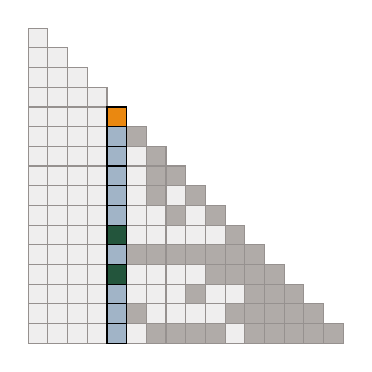
\begin{tikzpicture}[scale=4/16]
  \filldraw[draw=zeroborder, fill=zerocolor] (0, 0) rectangle (1, -1);
  \filldraw[draw=zeroborder, fill=zerocolor] (0, -1) rectangle (1, -2);
  \filldraw[draw=zeroborder, fill=zerocolor] (0, -2) rectangle (1, -3);
  \filldraw[draw=zeroborder, fill=zerocolor] (0, -3) rectangle (1, -4);
  \filldraw[draw=zeroborder, fill=zerocolor] (0, -4) rectangle (1, -5);
  \filldraw[draw=zeroborder, fill=zerocolor] (0, -5) rectangle (1, -6);
  \filldraw[draw=zeroborder, fill=zerocolor] (0, -6) rectangle (1, -7);
  \filldraw[draw=zeroborder, fill=zerocolor] (0, -7) rectangle (1, -8);
  \filldraw[draw=zeroborder, fill=zerocolor] (0, -8) rectangle (1, -9);
  \filldraw[draw=zeroborder, fill=zerocolor] (0, -9) rectangle (1, -10);
  \filldraw[draw=zeroborder, fill=zerocolor] (0, -10) rectangle (1, -11);
  \filldraw[draw=zeroborder, fill=zerocolor] (0, -11) rectangle (1, -12);
  \filldraw[draw=zeroborder, fill=zerocolor] (0, -12) rectangle (1, -13);
  \filldraw[draw=zeroborder, fill=zerocolor] (0, -13) rectangle (1, -14);
  \filldraw[draw=zeroborder, fill=zerocolor] (0, -14) rectangle (1, -15);
  \filldraw[draw=zeroborder, fill=zerocolor] (0, -15) rectangle (1, -16);
  \filldraw[draw=zeroborder, fill=zerocolor] (1, -1) rectangle (2, -2);
  \filldraw[draw=zeroborder, fill=zerocolor] (1, -2) rectangle (2, -3);
  \filldraw[draw=zeroborder, fill=zerocolor] (1, -3) rectangle (2, -4);
  \filldraw[draw=zeroborder, fill=zerocolor] (1, -4) rectangle (2, -5);
  \filldraw[draw=zeroborder, fill=zerocolor] (1, -5) rectangle (2, -6);
  \filldraw[draw=zeroborder, fill=zerocolor] (1, -6) rectangle (2, -7);
  \filldraw[draw=zeroborder, fill=zerocolor] (1, -7) rectangle (2, -8);
  \filldraw[draw=zeroborder, fill=zerocolor] (1, -8) rectangle (2, -9);
  \filldraw[draw=zeroborder, fill=zerocolor] (1, -9) rectangle (2, -10);
  \filldraw[draw=zeroborder, fill=zerocolor] (1, -10) rectangle (2, -11);
  \filldraw[draw=zeroborder, fill=zerocolor] (1, -11) rectangle (2, -12);
  \filldraw[draw=zeroborder, fill=zerocolor] (1, -12) rectangle (2, -13);
  \filldraw[draw=zeroborder, fill=zerocolor] (1, -13) rectangle (2, -14);
  \filldraw[draw=zeroborder, fill=zerocolor] (1, -14) rectangle (2, -15);
  \filldraw[draw=zeroborder, fill=zerocolor] (1, -15) rectangle (2, -16);
  \filldraw[draw=zeroborder, fill=zerocolor] (2, -2) rectangle (3, -3);
  \filldraw[draw=zeroborder, fill=zerocolor] (2, -3) rectangle (3, -4);
  \filldraw[draw=zeroborder, fill=zerocolor] (2, -4) rectangle (3, -5);
  \filldraw[draw=zeroborder, fill=zerocolor] (2, -5) rectangle (3, -6);
  \filldraw[draw=zeroborder, fill=zerocolor] (2, -6) rectangle (3, -7);
  \filldraw[draw=zeroborder, fill=zerocolor] (2, -7) rectangle (3, -8);
  \filldraw[draw=zeroborder, fill=zerocolor] (2, -8) rectangle (3, -9);
  \filldraw[draw=zeroborder, fill=zerocolor] (2, -9) rectangle (3, -10);
  \filldraw[draw=zeroborder, fill=zerocolor] (2, -10) rectangle (3, -11);
  \filldraw[draw=zeroborder, fill=zerocolor] (2, -11) rectangle (3, -12);
  \filldraw[draw=zeroborder, fill=zerocolor] (2, -12) rectangle (3, -13);
  \filldraw[draw=zeroborder, fill=zerocolor] (2, -13) rectangle (3, -14);
  \filldraw[draw=zeroborder, fill=zerocolor] (2, -14) rectangle (3, -15);
  \filldraw[draw=zeroborder, fill=zerocolor] (2, -15) rectangle (3, -16);
  \filldraw[draw=zeroborder, fill=zerocolor] (3, -3) rectangle (4, -4);
  \filldraw[draw=zeroborder, fill=zerocolor] (3, -4) rectangle (4, -5);
  \filldraw[draw=zeroborder, fill=zerocolor] (3, -5) rectangle (4, -6);
  \filldraw[draw=zeroborder, fill=zerocolor] (3, -6) rectangle (4, -7);
  \filldraw[draw=zeroborder, fill=zerocolor] (3, -7) rectangle (4, -8);
  \filldraw[draw=zeroborder, fill=zerocolor] (3, -8) rectangle (4, -9);
  \filldraw[draw=zeroborder, fill=zerocolor] (3, -9) rectangle (4, -10);
  \filldraw[draw=zeroborder, fill=zerocolor] (3, -10) rectangle (4, -11);
  \filldraw[draw=zeroborder, fill=zerocolor] (3, -11) rectangle (4, -12);
  \filldraw[draw=zeroborder, fill=zerocolor] (3, -12) rectangle (4, -13);
  \filldraw[draw=zeroborder, fill=zerocolor] (3, -13) rectangle (4, -14);
  \filldraw[draw=zeroborder, fill=zerocolor] (3, -14) rectangle (4, -15);
  \filldraw[draw=zeroborder, fill=zerocolor] (3, -15) rectangle (4, -16);
  \filldraw[draw=nnzborder, fill=nnzcolor] (5, -5) rectangle (6, -6);
  \filldraw[draw=zeroborder, fill=zerocolor] (5, -6) rectangle (6, -7);
  \filldraw[draw=zeroborder, fill=zerocolor] (5, -7) rectangle (6, -8);
  \filldraw[draw=zeroborder, fill=zerocolor] (5, -8) rectangle (6, -9);
  \filldraw[draw=zeroborder, fill=zerocolor] (5, -9) rectangle (6, -10);
  \filldraw[draw=zeroborder, fill=zerocolor] (5, -10) rectangle (6, -11);
  \filldraw[draw=nnzborder, fill=nnzcolor] (5, -11) rectangle (6, -12);
  \filldraw[draw=zeroborder, fill=zerocolor] (5, -12) rectangle (6, -13);
  \filldraw[draw=zeroborder, fill=zerocolor] (5, -13) rectangle (6, -14);
  \filldraw[draw=nnzborder, fill=nnzcolor] (5, -14) rectangle (6, -15);
  \filldraw[draw=zeroborder, fill=zerocolor] (5, -15) rectangle (6, -16);
  \filldraw[draw=nnzborder, fill=nnzcolor] (6, -6) rectangle (7, -7);
  \filldraw[draw=nnzborder, fill=nnzcolor] (6, -7) rectangle (7, -8);
  \filldraw[draw=nnzborder, fill=nnzcolor] (6, -8) rectangle (7, -9);
  \filldraw[draw=zeroborder, fill=zerocolor] (6, -9) rectangle (7, -10);
  \filldraw[draw=zeroborder, fill=zerocolor] (6, -10) rectangle (7, -11);
  \filldraw[draw=nnzborder, fill=nnzcolor] (6, -11) rectangle (7, -12);
  \filldraw[draw=zeroborder, fill=zerocolor] (6, -12) rectangle (7, -13);
  \filldraw[draw=zeroborder, fill=zerocolor] (6, -13) rectangle (7, -14);
  \filldraw[draw=zeroborder, fill=zerocolor] (6, -14) rectangle (7, -15);
  \filldraw[draw=nnzborder, fill=nnzcolor] (6, -15) rectangle (7, -16);
  \filldraw[draw=nnzborder, fill=nnzcolor] (7, -7) rectangle (8, -8);
  \filldraw[draw=zeroborder, fill=zerocolor] (7, -8) rectangle (8, -9);
  \filldraw[draw=nnzborder, fill=nnzcolor] (7, -9) rectangle (8, -10);
  \filldraw[draw=zeroborder, fill=zerocolor] (7, -10) rectangle (8, -11);
  \filldraw[draw=nnzborder, fill=nnzcolor] (7, -11) rectangle (8, -12);
  \filldraw[draw=zeroborder, fill=zerocolor] (7, -12) rectangle (8, -13);
  \filldraw[draw=zeroborder, fill=zerocolor] (7, -13) rectangle (8, -14);
  \filldraw[draw=zeroborder, fill=zerocolor] (7, -14) rectangle (8, -15);
  \filldraw[draw=nnzborder, fill=nnzcolor] (7, -15) rectangle (8, -16);
  \filldraw[draw=nnzborder, fill=nnzcolor] (8, -8) rectangle (9, -9);
  \filldraw[draw=zeroborder, fill=zerocolor] (8, -9) rectangle (9, -10);
  \filldraw[draw=zeroborder, fill=zerocolor] (8, -10) rectangle (9, -11);
  \filldraw[draw=nnzborder, fill=nnzcolor] (8, -11) rectangle (9, -12);
  \filldraw[draw=zeroborder, fill=zerocolor] (8, -12) rectangle (9, -13);
  \filldraw[draw=nnzborder, fill=nnzcolor] (8, -13) rectangle (9, -14);
  \filldraw[draw=zeroborder, fill=zerocolor] (8, -14) rectangle (9, -15);
  \filldraw[draw=nnzborder, fill=nnzcolor] (8, -15) rectangle (9, -16);
  \filldraw[draw=nnzborder, fill=nnzcolor] (9, -9) rectangle (10, -10);
  \filldraw[draw=zeroborder, fill=zerocolor] (9, -10) rectangle (10, -11);
  \filldraw[draw=nnzborder, fill=nnzcolor] (9, -11) rectangle (10, -12);
  \filldraw[draw=nnzborder, fill=nnzcolor] (9, -12) rectangle (10, -13);
  \filldraw[draw=zeroborder, fill=zerocolor] (9, -13) rectangle (10, -14);
  \filldraw[draw=zeroborder, fill=zerocolor] (9, -14) rectangle (10, -15);
  \filldraw[draw=nnzborder, fill=nnzcolor] (9, -15) rectangle (10, -16);
  \filldraw[draw=nnzborder, fill=nnzcolor] (10, -10) rectangle (11, -11);
  \filldraw[draw=nnzborder, fill=nnzcolor] (10, -11) rectangle (11, -12);
  \filldraw[draw=nnzborder, fill=nnzcolor] (10, -12) rectangle (11, -13);
  \filldraw[draw=zeroborder, fill=zerocolor] (10, -13) rectangle (11, -14);
  \filldraw[draw=nnzborder, fill=nnzcolor] (10, -14) rectangle (11, -15);
  \filldraw[draw=zeroborder, fill=zerocolor] (10, -15) rectangle (11, -16);
  \filldraw[draw=nnzborder, fill=nnzcolor] (11, -11) rectangle (12, -12);
  \filldraw[draw=nnzborder, fill=nnzcolor] (11, -12) rectangle (12, -13);
  \filldraw[draw=nnzborder, fill=nnzcolor] (11, -13) rectangle (12, -14);
  \filldraw[draw=nnzborder, fill=nnzcolor] (11, -14) rectangle (12, -15);
  \filldraw[draw=nnzborder, fill=nnzcolor] (11, -15) rectangle (12, -16);
  \filldraw[draw=nnzborder, fill=nnzcolor] (12, -12) rectangle (13, -13);
  \filldraw[draw=nnzborder, fill=nnzcolor] (12, -13) rectangle (13, -14);
  \filldraw[draw=nnzborder, fill=nnzcolor] (12, -14) rectangle (13, -15);
  \filldraw[draw=nnzborder, fill=nnzcolor] (12, -15) rectangle (13, -16);
  \filldraw[draw=nnzborder, fill=nnzcolor] (13, -13) rectangle (14, -14);
  \filldraw[draw=nnzborder, fill=nnzcolor] (13, -14) rectangle (14, -15);
  \filldraw[draw=nnzborder, fill=nnzcolor] (13, -15) rectangle (14, -16);
  \filldraw[draw=nnzborder, fill=nnzcolor] (14, -14) rectangle (15, -15);
  \filldraw[draw=nnzborder, fill=nnzcolor] (14, -15) rectangle (15, -16);
  \filldraw[draw=nnzborder, fill=nnzcolor] (15, -15) rectangle (16, -16);
  \filldraw[draw=colborder, fill=targetcolor] (4, -4) rectangle (5, -5);
  \filldraw[draw=colborder, fill=candcolor] (4, -5) rectangle (5, -6);
  \filldraw[draw=colborder, fill=candcolor] (4, -6) rectangle (5, -7);
  \filldraw[draw=colborder, fill=candcolor] (4, -7) rectangle (5, -8);
  \filldraw[draw=colborder, fill=candcolor] (4, -8) rectangle (5, -9);
  \filldraw[draw=colborder, fill=candcolor] (4, -9) rectangle (5, -10);
  \filldraw[draw=colborder, fill=selcolor] (4, -10) rectangle (5, -11);
  \filldraw[draw=colborder, fill=candcolor] (4, -11) rectangle (5, -12);
  \filldraw[draw=colborder, fill=selcolor] (4, -12) rectangle (5, -13);
  \filldraw[draw=colborder, fill=candcolor] (4, -13) rectangle (5, -14);
  \filldraw[draw=colborder, fill=candcolor] (4, -14) rectangle (5, -15);
  \filldraw[draw=colborder, fill=candcolor] (4, -15) rectangle (5, -16);
\end{tikzpicture}
%
    \qquad
    \begin{tikzpicture}[baseline]
  \begin{axis}[
    % calculated from Cholesky factor, exactly 16 cm x 16 cm
    width={4cm},
    height={4cm},
    axis lines={none},
    % force axis box to have exactly the right dimensions, ignoring labels
    scale only axis=true,
  ]
  % consistent size bounding box
  \draw [white, line width=0] (-0.1, -0.1) -- (-0.1,  1.1);
  \draw [white, line width=0] ( 1.1, -0.1) -- ( 1.1,  1.1);
  \draw [white, line width=0] (-0.1, -0.1) -- (-1.1, -0.1);
  \draw [white, line width=0] (-0.1,  1.1) -- (-1.1,  1.1);
  \draw [seagreen!15, fill, radius=0.3662240505218506] (0.6962159966701554, 0.2927207490124871) circle;
  \draw [seagreen, radius=0.3662240505218506] (0.6962159966701554, 0.2927207490124871) circle;
  \draw [orange!25, fill, radius=0.1831120252609253] (0.6962159966701554, 0.2927207490124871) circle;
  \draw [orange, radius=0.1831120252609253] (0.6962159966701554, 0.2927207490124871) circle;
  \addplot [only marks, mark size=1, silver]    table
    {figures/points_knn/all_points.csv};
  \addplot [only marks, mark size=2, lightblue] table
    {figures/points_knn/candidates_12.csv};
  \addplot [only marks, mark size=4, seagreen]  table
    {figures/points_knn/selected_12.csv};
  \addplot [only marks, mark size=4, orange]    table
    {figures/points_knn/target_12.csv};
  \end{axis}
\end{tikzpicture}

  \end{figure}
}
\only<13>{
  \begin{figure}
    \centering
    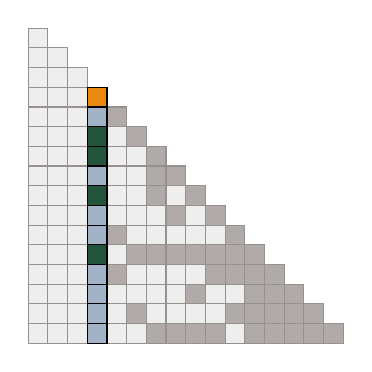
\begin{tikzpicture}[scale=4/16]
  \filldraw[draw=zeroborder, fill=zerocolor] (0, 0) rectangle (1, -1);
  \filldraw[draw=zeroborder, fill=zerocolor] (0, -1) rectangle (1, -2);
  \filldraw[draw=zeroborder, fill=zerocolor] (0, -2) rectangle (1, -3);
  \filldraw[draw=zeroborder, fill=zerocolor] (0, -3) rectangle (1, -4);
  \filldraw[draw=zeroborder, fill=zerocolor] (0, -4) rectangle (1, -5);
  \filldraw[draw=zeroborder, fill=zerocolor] (0, -5) rectangle (1, -6);
  \filldraw[draw=zeroborder, fill=zerocolor] (0, -6) rectangle (1, -7);
  \filldraw[draw=zeroborder, fill=zerocolor] (0, -7) rectangle (1, -8);
  \filldraw[draw=zeroborder, fill=zerocolor] (0, -8) rectangle (1, -9);
  \filldraw[draw=zeroborder, fill=zerocolor] (0, -9) rectangle (1, -10);
  \filldraw[draw=zeroborder, fill=zerocolor] (0, -10) rectangle (1, -11);
  \filldraw[draw=zeroborder, fill=zerocolor] (0, -11) rectangle (1, -12);
  \filldraw[draw=zeroborder, fill=zerocolor] (0, -12) rectangle (1, -13);
  \filldraw[draw=zeroborder, fill=zerocolor] (0, -13) rectangle (1, -14);
  \filldraw[draw=zeroborder, fill=zerocolor] (0, -14) rectangle (1, -15);
  \filldraw[draw=zeroborder, fill=zerocolor] (0, -15) rectangle (1, -16);
  \filldraw[draw=zeroborder, fill=zerocolor] (1, -1) rectangle (2, -2);
  \filldraw[draw=zeroborder, fill=zerocolor] (1, -2) rectangle (2, -3);
  \filldraw[draw=zeroborder, fill=zerocolor] (1, -3) rectangle (2, -4);
  \filldraw[draw=zeroborder, fill=zerocolor] (1, -4) rectangle (2, -5);
  \filldraw[draw=zeroborder, fill=zerocolor] (1, -5) rectangle (2, -6);
  \filldraw[draw=zeroborder, fill=zerocolor] (1, -6) rectangle (2, -7);
  \filldraw[draw=zeroborder, fill=zerocolor] (1, -7) rectangle (2, -8);
  \filldraw[draw=zeroborder, fill=zerocolor] (1, -8) rectangle (2, -9);
  \filldraw[draw=zeroborder, fill=zerocolor] (1, -9) rectangle (2, -10);
  \filldraw[draw=zeroborder, fill=zerocolor] (1, -10) rectangle (2, -11);
  \filldraw[draw=zeroborder, fill=zerocolor] (1, -11) rectangle (2, -12);
  \filldraw[draw=zeroborder, fill=zerocolor] (1, -12) rectangle (2, -13);
  \filldraw[draw=zeroborder, fill=zerocolor] (1, -13) rectangle (2, -14);
  \filldraw[draw=zeroborder, fill=zerocolor] (1, -14) rectangle (2, -15);
  \filldraw[draw=zeroborder, fill=zerocolor] (1, -15) rectangle (2, -16);
  \filldraw[draw=zeroborder, fill=zerocolor] (2, -2) rectangle (3, -3);
  \filldraw[draw=zeroborder, fill=zerocolor] (2, -3) rectangle (3, -4);
  \filldraw[draw=zeroborder, fill=zerocolor] (2, -4) rectangle (3, -5);
  \filldraw[draw=zeroborder, fill=zerocolor] (2, -5) rectangle (3, -6);
  \filldraw[draw=zeroborder, fill=zerocolor] (2, -6) rectangle (3, -7);
  \filldraw[draw=zeroborder, fill=zerocolor] (2, -7) rectangle (3, -8);
  \filldraw[draw=zeroborder, fill=zerocolor] (2, -8) rectangle (3, -9);
  \filldraw[draw=zeroborder, fill=zerocolor] (2, -9) rectangle (3, -10);
  \filldraw[draw=zeroborder, fill=zerocolor] (2, -10) rectangle (3, -11);
  \filldraw[draw=zeroborder, fill=zerocolor] (2, -11) rectangle (3, -12);
  \filldraw[draw=zeroborder, fill=zerocolor] (2, -12) rectangle (3, -13);
  \filldraw[draw=zeroborder, fill=zerocolor] (2, -13) rectangle (3, -14);
  \filldraw[draw=zeroborder, fill=zerocolor] (2, -14) rectangle (3, -15);
  \filldraw[draw=zeroborder, fill=zerocolor] (2, -15) rectangle (3, -16);
  \filldraw[draw=nnzborder, fill=nnzcolor] (4, -4) rectangle (5, -5);
  \filldraw[draw=zeroborder, fill=zerocolor] (4, -5) rectangle (5, -6);
  \filldraw[draw=zeroborder, fill=zerocolor] (4, -6) rectangle (5, -7);
  \filldraw[draw=zeroborder, fill=zerocolor] (4, -7) rectangle (5, -8);
  \filldraw[draw=zeroborder, fill=zerocolor] (4, -8) rectangle (5, -9);
  \filldraw[draw=zeroborder, fill=zerocolor] (4, -9) rectangle (5, -10);
  \filldraw[draw=nnzborder, fill=nnzcolor] (4, -10) rectangle (5, -11);
  \filldraw[draw=zeroborder, fill=zerocolor] (4, -11) rectangle (5, -12);
  \filldraw[draw=nnzborder, fill=nnzcolor] (4, -12) rectangle (5, -13);
  \filldraw[draw=zeroborder, fill=zerocolor] (4, -13) rectangle (5, -14);
  \filldraw[draw=zeroborder, fill=zerocolor] (4, -14) rectangle (5, -15);
  \filldraw[draw=zeroborder, fill=zerocolor] (4, -15) rectangle (5, -16);
  \filldraw[draw=nnzborder, fill=nnzcolor] (5, -5) rectangle (6, -6);
  \filldraw[draw=zeroborder, fill=zerocolor] (5, -6) rectangle (6, -7);
  \filldraw[draw=zeroborder, fill=zerocolor] (5, -7) rectangle (6, -8);
  \filldraw[draw=zeroborder, fill=zerocolor] (5, -8) rectangle (6, -9);
  \filldraw[draw=zeroborder, fill=zerocolor] (5, -9) rectangle (6, -10);
  \filldraw[draw=zeroborder, fill=zerocolor] (5, -10) rectangle (6, -11);
  \filldraw[draw=nnzborder, fill=nnzcolor] (5, -11) rectangle (6, -12);
  \filldraw[draw=zeroborder, fill=zerocolor] (5, -12) rectangle (6, -13);
  \filldraw[draw=zeroborder, fill=zerocolor] (5, -13) rectangle (6, -14);
  \filldraw[draw=nnzborder, fill=nnzcolor] (5, -14) rectangle (6, -15);
  \filldraw[draw=zeroborder, fill=zerocolor] (5, -15) rectangle (6, -16);
  \filldraw[draw=nnzborder, fill=nnzcolor] (6, -6) rectangle (7, -7);
  \filldraw[draw=nnzborder, fill=nnzcolor] (6, -7) rectangle (7, -8);
  \filldraw[draw=nnzborder, fill=nnzcolor] (6, -8) rectangle (7, -9);
  \filldraw[draw=zeroborder, fill=zerocolor] (6, -9) rectangle (7, -10);
  \filldraw[draw=zeroborder, fill=zerocolor] (6, -10) rectangle (7, -11);
  \filldraw[draw=nnzborder, fill=nnzcolor] (6, -11) rectangle (7, -12);
  \filldraw[draw=zeroborder, fill=zerocolor] (6, -12) rectangle (7, -13);
  \filldraw[draw=zeroborder, fill=zerocolor] (6, -13) rectangle (7, -14);
  \filldraw[draw=zeroborder, fill=zerocolor] (6, -14) rectangle (7, -15);
  \filldraw[draw=nnzborder, fill=nnzcolor] (6, -15) rectangle (7, -16);
  \filldraw[draw=nnzborder, fill=nnzcolor] (7, -7) rectangle (8, -8);
  \filldraw[draw=zeroborder, fill=zerocolor] (7, -8) rectangle (8, -9);
  \filldraw[draw=nnzborder, fill=nnzcolor] (7, -9) rectangle (8, -10);
  \filldraw[draw=zeroborder, fill=zerocolor] (7, -10) rectangle (8, -11);
  \filldraw[draw=nnzborder, fill=nnzcolor] (7, -11) rectangle (8, -12);
  \filldraw[draw=zeroborder, fill=zerocolor] (7, -12) rectangle (8, -13);
  \filldraw[draw=zeroborder, fill=zerocolor] (7, -13) rectangle (8, -14);
  \filldraw[draw=zeroborder, fill=zerocolor] (7, -14) rectangle (8, -15);
  \filldraw[draw=nnzborder, fill=nnzcolor] (7, -15) rectangle (8, -16);
  \filldraw[draw=nnzborder, fill=nnzcolor] (8, -8) rectangle (9, -9);
  \filldraw[draw=zeroborder, fill=zerocolor] (8, -9) rectangle (9, -10);
  \filldraw[draw=zeroborder, fill=zerocolor] (8, -10) rectangle (9, -11);
  \filldraw[draw=nnzborder, fill=nnzcolor] (8, -11) rectangle (9, -12);
  \filldraw[draw=zeroborder, fill=zerocolor] (8, -12) rectangle (9, -13);
  \filldraw[draw=nnzborder, fill=nnzcolor] (8, -13) rectangle (9, -14);
  \filldraw[draw=zeroborder, fill=zerocolor] (8, -14) rectangle (9, -15);
  \filldraw[draw=nnzborder, fill=nnzcolor] (8, -15) rectangle (9, -16);
  \filldraw[draw=nnzborder, fill=nnzcolor] (9, -9) rectangle (10, -10);
  \filldraw[draw=zeroborder, fill=zerocolor] (9, -10) rectangle (10, -11);
  \filldraw[draw=nnzborder, fill=nnzcolor] (9, -11) rectangle (10, -12);
  \filldraw[draw=nnzborder, fill=nnzcolor] (9, -12) rectangle (10, -13);
  \filldraw[draw=zeroborder, fill=zerocolor] (9, -13) rectangle (10, -14);
  \filldraw[draw=zeroborder, fill=zerocolor] (9, -14) rectangle (10, -15);
  \filldraw[draw=nnzborder, fill=nnzcolor] (9, -15) rectangle (10, -16);
  \filldraw[draw=nnzborder, fill=nnzcolor] (10, -10) rectangle (11, -11);
  \filldraw[draw=nnzborder, fill=nnzcolor] (10, -11) rectangle (11, -12);
  \filldraw[draw=nnzborder, fill=nnzcolor] (10, -12) rectangle (11, -13);
  \filldraw[draw=zeroborder, fill=zerocolor] (10, -13) rectangle (11, -14);
  \filldraw[draw=nnzborder, fill=nnzcolor] (10, -14) rectangle (11, -15);
  \filldraw[draw=zeroborder, fill=zerocolor] (10, -15) rectangle (11, -16);
  \filldraw[draw=nnzborder, fill=nnzcolor] (11, -11) rectangle (12, -12);
  \filldraw[draw=nnzborder, fill=nnzcolor] (11, -12) rectangle (12, -13);
  \filldraw[draw=nnzborder, fill=nnzcolor] (11, -13) rectangle (12, -14);
  \filldraw[draw=nnzborder, fill=nnzcolor] (11, -14) rectangle (12, -15);
  \filldraw[draw=nnzborder, fill=nnzcolor] (11, -15) rectangle (12, -16);
  \filldraw[draw=nnzborder, fill=nnzcolor] (12, -12) rectangle (13, -13);
  \filldraw[draw=nnzborder, fill=nnzcolor] (12, -13) rectangle (13, -14);
  \filldraw[draw=nnzborder, fill=nnzcolor] (12, -14) rectangle (13, -15);
  \filldraw[draw=nnzborder, fill=nnzcolor] (12, -15) rectangle (13, -16);
  \filldraw[draw=nnzborder, fill=nnzcolor] (13, -13) rectangle (14, -14);
  \filldraw[draw=nnzborder, fill=nnzcolor] (13, -14) rectangle (14, -15);
  \filldraw[draw=nnzborder, fill=nnzcolor] (13, -15) rectangle (14, -16);
  \filldraw[draw=nnzborder, fill=nnzcolor] (14, -14) rectangle (15, -15);
  \filldraw[draw=nnzborder, fill=nnzcolor] (14, -15) rectangle (15, -16);
  \filldraw[draw=nnzborder, fill=nnzcolor] (15, -15) rectangle (16, -16);
  \filldraw[draw=colborder, fill=targetcolor] (3, -3) rectangle (4, -4);
  \filldraw[draw=colborder, fill=candcolor] (3, -4) rectangle (4, -5);
  \filldraw[draw=colborder, fill=selcolor] (3, -5) rectangle (4, -6);
  \filldraw[draw=colborder, fill=selcolor] (3, -6) rectangle (4, -7);
  \filldraw[draw=colborder, fill=candcolor] (3, -7) rectangle (4, -8);
  \filldraw[draw=colborder, fill=selcolor] (3, -8) rectangle (4, -9);
  \filldraw[draw=colborder, fill=candcolor] (3, -9) rectangle (4, -10);
  \filldraw[draw=colborder, fill=candcolor] (3, -10) rectangle (4, -11);
  \filldraw[draw=colborder, fill=selcolor] (3, -11) rectangle (4, -12);
  \filldraw[draw=colborder, fill=candcolor] (3, -12) rectangle (4, -13);
  \filldraw[draw=colborder, fill=candcolor] (3, -13) rectangle (4, -14);
  \filldraw[draw=colborder, fill=candcolor] (3, -14) rectangle (4, -15);
  \filldraw[draw=colborder, fill=candcolor] (3, -15) rectangle (4, -16);
\end{tikzpicture}
%
    \qquad
    \begin{tikzpicture}[baseline]
  \begin{axis}[
    % calculated from Cholesky factor, exactly 16 cm x 16 cm
    width={4cm},
    height={4cm},
    axis lines={none},
    % force axis box to have exactly the right dimensions, ignoring labels
    scale only axis=true,
  ]
  % consistent size bounding box
  \draw [white, line width=0] (-0.1, -0.1) -- (-0.1,  1.1);
  \draw [white, line width=0] ( 1.1, -0.1) -- ( 1.1,  1.1);
  \draw [white, line width=0] (-0.1, -0.1) -- (-1.1, -0.1);
  \draw [white, line width=0] (-0.1,  1.1) -- (-1.1,  1.1);
  \addplot [only marks, mark size=1, silver]    table
    {figures/points_cknn/all_points.csv};
  \addplot [only marks, mark size=2, lightblue] table
    {figures/points_cknn/candidates.csv};
  \addplot [only marks, mark size=4, seagreen]  table
    {figures/points_cknn/selected_13.csv};
  \addplot [only marks, mark size=4, orange]    table
    {figures/points_cknn/target.csv};
  \end{axis}
\end{tikzpicture}

  \end{figure}
}
\only<14>{
  \begin{figure}
    \centering
    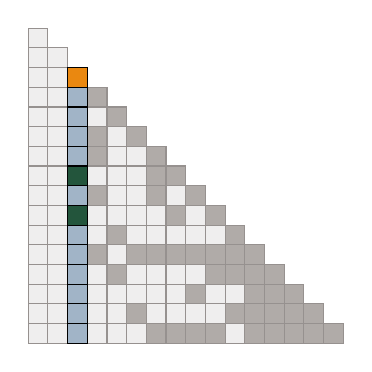
\begin{tikzpicture}[scale=4/16]
  \filldraw[draw=zeroborder, fill=zerocolor] (0, 0) rectangle (1, -1);
  \filldraw[draw=zeroborder, fill=zerocolor] (0, -1) rectangle (1, -2);
  \filldraw[draw=zeroborder, fill=zerocolor] (0, -2) rectangle (1, -3);
  \filldraw[draw=zeroborder, fill=zerocolor] (0, -3) rectangle (1, -4);
  \filldraw[draw=zeroborder, fill=zerocolor] (0, -4) rectangle (1, -5);
  \filldraw[draw=zeroborder, fill=zerocolor] (0, -5) rectangle (1, -6);
  \filldraw[draw=zeroborder, fill=zerocolor] (0, -6) rectangle (1, -7);
  \filldraw[draw=zeroborder, fill=zerocolor] (0, -7) rectangle (1, -8);
  \filldraw[draw=zeroborder, fill=zerocolor] (0, -8) rectangle (1, -9);
  \filldraw[draw=zeroborder, fill=zerocolor] (0, -9) rectangle (1, -10);
  \filldraw[draw=zeroborder, fill=zerocolor] (0, -10) rectangle (1, -11);
  \filldraw[draw=zeroborder, fill=zerocolor] (0, -11) rectangle (1, -12);
  \filldraw[draw=zeroborder, fill=zerocolor] (0, -12) rectangle (1, -13);
  \filldraw[draw=zeroborder, fill=zerocolor] (0, -13) rectangle (1, -14);
  \filldraw[draw=zeroborder, fill=zerocolor] (0, -14) rectangle (1, -15);
  \filldraw[draw=zeroborder, fill=zerocolor] (0, -15) rectangle (1, -16);
  \filldraw[draw=zeroborder, fill=zerocolor] (1, -1) rectangle (2, -2);
  \filldraw[draw=zeroborder, fill=zerocolor] (1, -2) rectangle (2, -3);
  \filldraw[draw=zeroborder, fill=zerocolor] (1, -3) rectangle (2, -4);
  \filldraw[draw=zeroborder, fill=zerocolor] (1, -4) rectangle (2, -5);
  \filldraw[draw=zeroborder, fill=zerocolor] (1, -5) rectangle (2, -6);
  \filldraw[draw=zeroborder, fill=zerocolor] (1, -6) rectangle (2, -7);
  \filldraw[draw=zeroborder, fill=zerocolor] (1, -7) rectangle (2, -8);
  \filldraw[draw=zeroborder, fill=zerocolor] (1, -8) rectangle (2, -9);
  \filldraw[draw=zeroborder, fill=zerocolor] (1, -9) rectangle (2, -10);
  \filldraw[draw=zeroborder, fill=zerocolor] (1, -10) rectangle (2, -11);
  \filldraw[draw=zeroborder, fill=zerocolor] (1, -11) rectangle (2, -12);
  \filldraw[draw=zeroborder, fill=zerocolor] (1, -12) rectangle (2, -13);
  \filldraw[draw=zeroborder, fill=zerocolor] (1, -13) rectangle (2, -14);
  \filldraw[draw=zeroborder, fill=zerocolor] (1, -14) rectangle (2, -15);
  \filldraw[draw=zeroborder, fill=zerocolor] (1, -15) rectangle (2, -16);
  \filldraw[draw=nnzborder, fill=nnzcolor] (3, -3) rectangle (4, -4);
  \filldraw[draw=zeroborder, fill=zerocolor] (3, -4) rectangle (4, -5);
  \filldraw[draw=nnzborder, fill=nnzcolor] (3, -5) rectangle (4, -6);
  \filldraw[draw=nnzborder, fill=nnzcolor] (3, -6) rectangle (4, -7);
  \filldraw[draw=zeroborder, fill=zerocolor] (3, -7) rectangle (4, -8);
  \filldraw[draw=nnzborder, fill=nnzcolor] (3, -8) rectangle (4, -9);
  \filldraw[draw=zeroborder, fill=zerocolor] (3, -9) rectangle (4, -10);
  \filldraw[draw=zeroborder, fill=zerocolor] (3, -10) rectangle (4, -11);
  \filldraw[draw=nnzborder, fill=nnzcolor] (3, -11) rectangle (4, -12);
  \filldraw[draw=zeroborder, fill=zerocolor] (3, -12) rectangle (4, -13);
  \filldraw[draw=zeroborder, fill=zerocolor] (3, -13) rectangle (4, -14);
  \filldraw[draw=zeroborder, fill=zerocolor] (3, -14) rectangle (4, -15);
  \filldraw[draw=zeroborder, fill=zerocolor] (3, -15) rectangle (4, -16);
  \filldraw[draw=nnzborder, fill=nnzcolor] (4, -4) rectangle (5, -5);
  \filldraw[draw=zeroborder, fill=zerocolor] (4, -5) rectangle (5, -6);
  \filldraw[draw=zeroborder, fill=zerocolor] (4, -6) rectangle (5, -7);
  \filldraw[draw=zeroborder, fill=zerocolor] (4, -7) rectangle (5, -8);
  \filldraw[draw=zeroborder, fill=zerocolor] (4, -8) rectangle (5, -9);
  \filldraw[draw=zeroborder, fill=zerocolor] (4, -9) rectangle (5, -10);
  \filldraw[draw=nnzborder, fill=nnzcolor] (4, -10) rectangle (5, -11);
  \filldraw[draw=zeroborder, fill=zerocolor] (4, -11) rectangle (5, -12);
  \filldraw[draw=nnzborder, fill=nnzcolor] (4, -12) rectangle (5, -13);
  \filldraw[draw=zeroborder, fill=zerocolor] (4, -13) rectangle (5, -14);
  \filldraw[draw=zeroborder, fill=zerocolor] (4, -14) rectangle (5, -15);
  \filldraw[draw=zeroborder, fill=zerocolor] (4, -15) rectangle (5, -16);
  \filldraw[draw=nnzborder, fill=nnzcolor] (5, -5) rectangle (6, -6);
  \filldraw[draw=zeroborder, fill=zerocolor] (5, -6) rectangle (6, -7);
  \filldraw[draw=zeroborder, fill=zerocolor] (5, -7) rectangle (6, -8);
  \filldraw[draw=zeroborder, fill=zerocolor] (5, -8) rectangle (6, -9);
  \filldraw[draw=zeroborder, fill=zerocolor] (5, -9) rectangle (6, -10);
  \filldraw[draw=zeroborder, fill=zerocolor] (5, -10) rectangle (6, -11);
  \filldraw[draw=nnzborder, fill=nnzcolor] (5, -11) rectangle (6, -12);
  \filldraw[draw=zeroborder, fill=zerocolor] (5, -12) rectangle (6, -13);
  \filldraw[draw=zeroborder, fill=zerocolor] (5, -13) rectangle (6, -14);
  \filldraw[draw=nnzborder, fill=nnzcolor] (5, -14) rectangle (6, -15);
  \filldraw[draw=zeroborder, fill=zerocolor] (5, -15) rectangle (6, -16);
  \filldraw[draw=nnzborder, fill=nnzcolor] (6, -6) rectangle (7, -7);
  \filldraw[draw=nnzborder, fill=nnzcolor] (6, -7) rectangle (7, -8);
  \filldraw[draw=nnzborder, fill=nnzcolor] (6, -8) rectangle (7, -9);
  \filldraw[draw=zeroborder, fill=zerocolor] (6, -9) rectangle (7, -10);
  \filldraw[draw=zeroborder, fill=zerocolor] (6, -10) rectangle (7, -11);
  \filldraw[draw=nnzborder, fill=nnzcolor] (6, -11) rectangle (7, -12);
  \filldraw[draw=zeroborder, fill=zerocolor] (6, -12) rectangle (7, -13);
  \filldraw[draw=zeroborder, fill=zerocolor] (6, -13) rectangle (7, -14);
  \filldraw[draw=zeroborder, fill=zerocolor] (6, -14) rectangle (7, -15);
  \filldraw[draw=nnzborder, fill=nnzcolor] (6, -15) rectangle (7, -16);
  \filldraw[draw=nnzborder, fill=nnzcolor] (7, -7) rectangle (8, -8);
  \filldraw[draw=zeroborder, fill=zerocolor] (7, -8) rectangle (8, -9);
  \filldraw[draw=nnzborder, fill=nnzcolor] (7, -9) rectangle (8, -10);
  \filldraw[draw=zeroborder, fill=zerocolor] (7, -10) rectangle (8, -11);
  \filldraw[draw=nnzborder, fill=nnzcolor] (7, -11) rectangle (8, -12);
  \filldraw[draw=zeroborder, fill=zerocolor] (7, -12) rectangle (8, -13);
  \filldraw[draw=zeroborder, fill=zerocolor] (7, -13) rectangle (8, -14);
  \filldraw[draw=zeroborder, fill=zerocolor] (7, -14) rectangle (8, -15);
  \filldraw[draw=nnzborder, fill=nnzcolor] (7, -15) rectangle (8, -16);
  \filldraw[draw=nnzborder, fill=nnzcolor] (8, -8) rectangle (9, -9);
  \filldraw[draw=zeroborder, fill=zerocolor] (8, -9) rectangle (9, -10);
  \filldraw[draw=zeroborder, fill=zerocolor] (8, -10) rectangle (9, -11);
  \filldraw[draw=nnzborder, fill=nnzcolor] (8, -11) rectangle (9, -12);
  \filldraw[draw=zeroborder, fill=zerocolor] (8, -12) rectangle (9, -13);
  \filldraw[draw=nnzborder, fill=nnzcolor] (8, -13) rectangle (9, -14);
  \filldraw[draw=zeroborder, fill=zerocolor] (8, -14) rectangle (9, -15);
  \filldraw[draw=nnzborder, fill=nnzcolor] (8, -15) rectangle (9, -16);
  \filldraw[draw=nnzborder, fill=nnzcolor] (9, -9) rectangle (10, -10);
  \filldraw[draw=zeroborder, fill=zerocolor] (9, -10) rectangle (10, -11);
  \filldraw[draw=nnzborder, fill=nnzcolor] (9, -11) rectangle (10, -12);
  \filldraw[draw=nnzborder, fill=nnzcolor] (9, -12) rectangle (10, -13);
  \filldraw[draw=zeroborder, fill=zerocolor] (9, -13) rectangle (10, -14);
  \filldraw[draw=zeroborder, fill=zerocolor] (9, -14) rectangle (10, -15);
  \filldraw[draw=nnzborder, fill=nnzcolor] (9, -15) rectangle (10, -16);
  \filldraw[draw=nnzborder, fill=nnzcolor] (10, -10) rectangle (11, -11);
  \filldraw[draw=nnzborder, fill=nnzcolor] (10, -11) rectangle (11, -12);
  \filldraw[draw=nnzborder, fill=nnzcolor] (10, -12) rectangle (11, -13);
  \filldraw[draw=zeroborder, fill=zerocolor] (10, -13) rectangle (11, -14);
  \filldraw[draw=nnzborder, fill=nnzcolor] (10, -14) rectangle (11, -15);
  \filldraw[draw=zeroborder, fill=zerocolor] (10, -15) rectangle (11, -16);
  \filldraw[draw=nnzborder, fill=nnzcolor] (11, -11) rectangle (12, -12);
  \filldraw[draw=nnzborder, fill=nnzcolor] (11, -12) rectangle (12, -13);
  \filldraw[draw=nnzborder, fill=nnzcolor] (11, -13) rectangle (12, -14);
  \filldraw[draw=nnzborder, fill=nnzcolor] (11, -14) rectangle (12, -15);
  \filldraw[draw=nnzborder, fill=nnzcolor] (11, -15) rectangle (12, -16);
  \filldraw[draw=nnzborder, fill=nnzcolor] (12, -12) rectangle (13, -13);
  \filldraw[draw=nnzborder, fill=nnzcolor] (12, -13) rectangle (13, -14);
  \filldraw[draw=nnzborder, fill=nnzcolor] (12, -14) rectangle (13, -15);
  \filldraw[draw=nnzborder, fill=nnzcolor] (12, -15) rectangle (13, -16);
  \filldraw[draw=nnzborder, fill=nnzcolor] (13, -13) rectangle (14, -14);
  \filldraw[draw=nnzborder, fill=nnzcolor] (13, -14) rectangle (14, -15);
  \filldraw[draw=nnzborder, fill=nnzcolor] (13, -15) rectangle (14, -16);
  \filldraw[draw=nnzborder, fill=nnzcolor] (14, -14) rectangle (15, -15);
  \filldraw[draw=nnzborder, fill=nnzcolor] (14, -15) rectangle (15, -16);
  \filldraw[draw=nnzborder, fill=nnzcolor] (15, -15) rectangle (16, -16);
  \filldraw[draw=colborder, fill=targetcolor] (2, -2) rectangle (3, -3);
  \filldraw[draw=colborder, fill=candcolor] (2, -3) rectangle (3, -4);
  \filldraw[draw=colborder, fill=candcolor] (2, -4) rectangle (3, -5);
  \filldraw[draw=colborder, fill=candcolor] (2, -5) rectangle (3, -6);
  \filldraw[draw=colborder, fill=candcolor] (2, -6) rectangle (3, -7);
  \filldraw[draw=colborder, fill=selcolor] (2, -7) rectangle (3, -8);
  \filldraw[draw=colborder, fill=candcolor] (2, -8) rectangle (3, -9);
  \filldraw[draw=colborder, fill=selcolor] (2, -9) rectangle (3, -10);
  \filldraw[draw=colborder, fill=candcolor] (2, -10) rectangle (3, -11);
  \filldraw[draw=colborder, fill=candcolor] (2, -11) rectangle (3, -12);
  \filldraw[draw=colborder, fill=candcolor] (2, -12) rectangle (3, -13);
  \filldraw[draw=colborder, fill=candcolor] (2, -13) rectangle (3, -14);
  \filldraw[draw=colborder, fill=candcolor] (2, -14) rectangle (3, -15);
  \filldraw[draw=colborder, fill=candcolor] (2, -15) rectangle (3, -16);
\end{tikzpicture}
%
    \qquad
    \begin{tikzpicture}[baseline]
  \begin{axis}[
    % calculated from Cholesky factor, exactly 16 cm x 16 cm
    width={4cm},
    height={4cm},
    axis lines={none},
    % force axis box to have exactly the right dimensions, ignoring labels
    scale only axis=true,
  ]
  % consistent size bounding box
  \draw [white, line width=0] (-0.1, -0.1) -- (-0.1,  1.1);
  \draw [white, line width=0] ( 1.1, -0.1) -- ( 1.1,  1.1);
  \draw [white, line width=0] (-0.1, -0.1) -- (-1.1, -0.1);
  \draw [white, line width=0] (-0.1,  1.1) -- (-1.1,  1.1);
  \draw [seagreen!15, fill, radius=0.2508378028869629] (0.479051298140834, 0.15973891463707857) circle;
  \draw [seagreen, radius=0.2508378028869629] (0.479051298140834, 0.15973891463707857) circle;
  \draw [orange!25, fill, radius=0.12541890144348145] (0.479051298140834, 0.15973891463707857) circle;
  \draw [orange, radius=0.12541890144348145] (0.479051298140834, 0.15973891463707857) circle;
  \addplot [only marks, mark size=1, silver]    table
    {figures/points_knn/all_points.csv};
  \addplot [only marks, mark size=2, lightblue] table
    {figures/points_knn/candidates_14.csv};
  \addplot [only marks, mark size=4, seagreen]  table
    {figures/points_knn/selected_14.csv};
  \addplot [only marks, mark size=4, orange]    table
    {figures/points_knn/target_14.csv};
  \end{axis}
\end{tikzpicture}

  \end{figure}
}
\only<15>{
  \begin{figure}
    \centering
    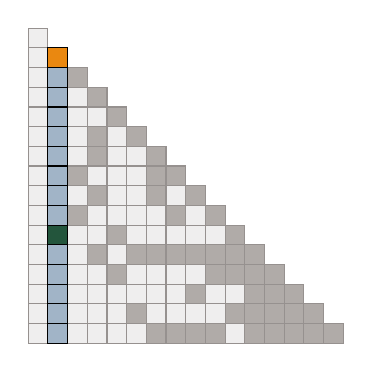
\begin{tikzpicture}[scale=4/16]
  \filldraw[draw=zeroborder, fill=zerocolor] (0, 0) rectangle (1, -1);
  \filldraw[draw=zeroborder, fill=zerocolor] (0, -1) rectangle (1, -2);
  \filldraw[draw=zeroborder, fill=zerocolor] (0, -2) rectangle (1, -3);
  \filldraw[draw=zeroborder, fill=zerocolor] (0, -3) rectangle (1, -4);
  \filldraw[draw=zeroborder, fill=zerocolor] (0, -4) rectangle (1, -5);
  \filldraw[draw=zeroborder, fill=zerocolor] (0, -5) rectangle (1, -6);
  \filldraw[draw=zeroborder, fill=zerocolor] (0, -6) rectangle (1, -7);
  \filldraw[draw=zeroborder, fill=zerocolor] (0, -7) rectangle (1, -8);
  \filldraw[draw=zeroborder, fill=zerocolor] (0, -8) rectangle (1, -9);
  \filldraw[draw=zeroborder, fill=zerocolor] (0, -9) rectangle (1, -10);
  \filldraw[draw=zeroborder, fill=zerocolor] (0, -10) rectangle (1, -11);
  \filldraw[draw=zeroborder, fill=zerocolor] (0, -11) rectangle (1, -12);
  \filldraw[draw=zeroborder, fill=zerocolor] (0, -12) rectangle (1, -13);
  \filldraw[draw=zeroborder, fill=zerocolor] (0, -13) rectangle (1, -14);
  \filldraw[draw=zeroborder, fill=zerocolor] (0, -14) rectangle (1, -15);
  \filldraw[draw=zeroborder, fill=zerocolor] (0, -15) rectangle (1, -16);
  \filldraw[draw=nnzborder, fill=nnzcolor] (2, -2) rectangle (3, -3);
  \filldraw[draw=zeroborder, fill=zerocolor] (2, -3) rectangle (3, -4);
  \filldraw[draw=zeroborder, fill=zerocolor] (2, -4) rectangle (3, -5);
  \filldraw[draw=zeroborder, fill=zerocolor] (2, -5) rectangle (3, -6);
  \filldraw[draw=zeroborder, fill=zerocolor] (2, -6) rectangle (3, -7);
  \filldraw[draw=nnzborder, fill=nnzcolor] (2, -7) rectangle (3, -8);
  \filldraw[draw=zeroborder, fill=zerocolor] (2, -8) rectangle (3, -9);
  \filldraw[draw=nnzborder, fill=nnzcolor] (2, -9) rectangle (3, -10);
  \filldraw[draw=zeroborder, fill=zerocolor] (2, -10) rectangle (3, -11);
  \filldraw[draw=zeroborder, fill=zerocolor] (2, -11) rectangle (3, -12);
  \filldraw[draw=zeroborder, fill=zerocolor] (2, -12) rectangle (3, -13);
  \filldraw[draw=zeroborder, fill=zerocolor] (2, -13) rectangle (3, -14);
  \filldraw[draw=zeroborder, fill=zerocolor] (2, -14) rectangle (3, -15);
  \filldraw[draw=zeroborder, fill=zerocolor] (2, -15) rectangle (3, -16);
  \filldraw[draw=nnzborder, fill=nnzcolor] (3, -3) rectangle (4, -4);
  \filldraw[draw=zeroborder, fill=zerocolor] (3, -4) rectangle (4, -5);
  \filldraw[draw=nnzborder, fill=nnzcolor] (3, -5) rectangle (4, -6);
  \filldraw[draw=nnzborder, fill=nnzcolor] (3, -6) rectangle (4, -7);
  \filldraw[draw=zeroborder, fill=zerocolor] (3, -7) rectangle (4, -8);
  \filldraw[draw=nnzborder, fill=nnzcolor] (3, -8) rectangle (4, -9);
  \filldraw[draw=zeroborder, fill=zerocolor] (3, -9) rectangle (4, -10);
  \filldraw[draw=zeroborder, fill=zerocolor] (3, -10) rectangle (4, -11);
  \filldraw[draw=nnzborder, fill=nnzcolor] (3, -11) rectangle (4, -12);
  \filldraw[draw=zeroborder, fill=zerocolor] (3, -12) rectangle (4, -13);
  \filldraw[draw=zeroborder, fill=zerocolor] (3, -13) rectangle (4, -14);
  \filldraw[draw=zeroborder, fill=zerocolor] (3, -14) rectangle (4, -15);
  \filldraw[draw=zeroborder, fill=zerocolor] (3, -15) rectangle (4, -16);
  \filldraw[draw=nnzborder, fill=nnzcolor] (4, -4) rectangle (5, -5);
  \filldraw[draw=zeroborder, fill=zerocolor] (4, -5) rectangle (5, -6);
  \filldraw[draw=zeroborder, fill=zerocolor] (4, -6) rectangle (5, -7);
  \filldraw[draw=zeroborder, fill=zerocolor] (4, -7) rectangle (5, -8);
  \filldraw[draw=zeroborder, fill=zerocolor] (4, -8) rectangle (5, -9);
  \filldraw[draw=zeroborder, fill=zerocolor] (4, -9) rectangle (5, -10);
  \filldraw[draw=nnzborder, fill=nnzcolor] (4, -10) rectangle (5, -11);
  \filldraw[draw=zeroborder, fill=zerocolor] (4, -11) rectangle (5, -12);
  \filldraw[draw=nnzborder, fill=nnzcolor] (4, -12) rectangle (5, -13);
  \filldraw[draw=zeroborder, fill=zerocolor] (4, -13) rectangle (5, -14);
  \filldraw[draw=zeroborder, fill=zerocolor] (4, -14) rectangle (5, -15);
  \filldraw[draw=zeroborder, fill=zerocolor] (4, -15) rectangle (5, -16);
  \filldraw[draw=nnzborder, fill=nnzcolor] (5, -5) rectangle (6, -6);
  \filldraw[draw=zeroborder, fill=zerocolor] (5, -6) rectangle (6, -7);
  \filldraw[draw=zeroborder, fill=zerocolor] (5, -7) rectangle (6, -8);
  \filldraw[draw=zeroborder, fill=zerocolor] (5, -8) rectangle (6, -9);
  \filldraw[draw=zeroborder, fill=zerocolor] (5, -9) rectangle (6, -10);
  \filldraw[draw=zeroborder, fill=zerocolor] (5, -10) rectangle (6, -11);
  \filldraw[draw=nnzborder, fill=nnzcolor] (5, -11) rectangle (6, -12);
  \filldraw[draw=zeroborder, fill=zerocolor] (5, -12) rectangle (6, -13);
  \filldraw[draw=zeroborder, fill=zerocolor] (5, -13) rectangle (6, -14);
  \filldraw[draw=nnzborder, fill=nnzcolor] (5, -14) rectangle (6, -15);
  \filldraw[draw=zeroborder, fill=zerocolor] (5, -15) rectangle (6, -16);
  \filldraw[draw=nnzborder, fill=nnzcolor] (6, -6) rectangle (7, -7);
  \filldraw[draw=nnzborder, fill=nnzcolor] (6, -7) rectangle (7, -8);
  \filldraw[draw=nnzborder, fill=nnzcolor] (6, -8) rectangle (7, -9);
  \filldraw[draw=zeroborder, fill=zerocolor] (6, -9) rectangle (7, -10);
  \filldraw[draw=zeroborder, fill=zerocolor] (6, -10) rectangle (7, -11);
  \filldraw[draw=nnzborder, fill=nnzcolor] (6, -11) rectangle (7, -12);
  \filldraw[draw=zeroborder, fill=zerocolor] (6, -12) rectangle (7, -13);
  \filldraw[draw=zeroborder, fill=zerocolor] (6, -13) rectangle (7, -14);
  \filldraw[draw=zeroborder, fill=zerocolor] (6, -14) rectangle (7, -15);
  \filldraw[draw=nnzborder, fill=nnzcolor] (6, -15) rectangle (7, -16);
  \filldraw[draw=nnzborder, fill=nnzcolor] (7, -7) rectangle (8, -8);
  \filldraw[draw=zeroborder, fill=zerocolor] (7, -8) rectangle (8, -9);
  \filldraw[draw=nnzborder, fill=nnzcolor] (7, -9) rectangle (8, -10);
  \filldraw[draw=zeroborder, fill=zerocolor] (7, -10) rectangle (8, -11);
  \filldraw[draw=nnzborder, fill=nnzcolor] (7, -11) rectangle (8, -12);
  \filldraw[draw=zeroborder, fill=zerocolor] (7, -12) rectangle (8, -13);
  \filldraw[draw=zeroborder, fill=zerocolor] (7, -13) rectangle (8, -14);
  \filldraw[draw=zeroborder, fill=zerocolor] (7, -14) rectangle (8, -15);
  \filldraw[draw=nnzborder, fill=nnzcolor] (7, -15) rectangle (8, -16);
  \filldraw[draw=nnzborder, fill=nnzcolor] (8, -8) rectangle (9, -9);
  \filldraw[draw=zeroborder, fill=zerocolor] (8, -9) rectangle (9, -10);
  \filldraw[draw=zeroborder, fill=zerocolor] (8, -10) rectangle (9, -11);
  \filldraw[draw=nnzborder, fill=nnzcolor] (8, -11) rectangle (9, -12);
  \filldraw[draw=zeroborder, fill=zerocolor] (8, -12) rectangle (9, -13);
  \filldraw[draw=nnzborder, fill=nnzcolor] (8, -13) rectangle (9, -14);
  \filldraw[draw=zeroborder, fill=zerocolor] (8, -14) rectangle (9, -15);
  \filldraw[draw=nnzborder, fill=nnzcolor] (8, -15) rectangle (9, -16);
  \filldraw[draw=nnzborder, fill=nnzcolor] (9, -9) rectangle (10, -10);
  \filldraw[draw=zeroborder, fill=zerocolor] (9, -10) rectangle (10, -11);
  \filldraw[draw=nnzborder, fill=nnzcolor] (9, -11) rectangle (10, -12);
  \filldraw[draw=nnzborder, fill=nnzcolor] (9, -12) rectangle (10, -13);
  \filldraw[draw=zeroborder, fill=zerocolor] (9, -13) rectangle (10, -14);
  \filldraw[draw=zeroborder, fill=zerocolor] (9, -14) rectangle (10, -15);
  \filldraw[draw=nnzborder, fill=nnzcolor] (9, -15) rectangle (10, -16);
  \filldraw[draw=nnzborder, fill=nnzcolor] (10, -10) rectangle (11, -11);
  \filldraw[draw=nnzborder, fill=nnzcolor] (10, -11) rectangle (11, -12);
  \filldraw[draw=nnzborder, fill=nnzcolor] (10, -12) rectangle (11, -13);
  \filldraw[draw=zeroborder, fill=zerocolor] (10, -13) rectangle (11, -14);
  \filldraw[draw=nnzborder, fill=nnzcolor] (10, -14) rectangle (11, -15);
  \filldraw[draw=zeroborder, fill=zerocolor] (10, -15) rectangle (11, -16);
  \filldraw[draw=nnzborder, fill=nnzcolor] (11, -11) rectangle (12, -12);
  \filldraw[draw=nnzborder, fill=nnzcolor] (11, -12) rectangle (12, -13);
  \filldraw[draw=nnzborder, fill=nnzcolor] (11, -13) rectangle (12, -14);
  \filldraw[draw=nnzborder, fill=nnzcolor] (11, -14) rectangle (12, -15);
  \filldraw[draw=nnzborder, fill=nnzcolor] (11, -15) rectangle (12, -16);
  \filldraw[draw=nnzborder, fill=nnzcolor] (12, -12) rectangle (13, -13);
  \filldraw[draw=nnzborder, fill=nnzcolor] (12, -13) rectangle (13, -14);
  \filldraw[draw=nnzborder, fill=nnzcolor] (12, -14) rectangle (13, -15);
  \filldraw[draw=nnzborder, fill=nnzcolor] (12, -15) rectangle (13, -16);
  \filldraw[draw=nnzborder, fill=nnzcolor] (13, -13) rectangle (14, -14);
  \filldraw[draw=nnzborder, fill=nnzcolor] (13, -14) rectangle (14, -15);
  \filldraw[draw=nnzborder, fill=nnzcolor] (13, -15) rectangle (14, -16);
  \filldraw[draw=nnzborder, fill=nnzcolor] (14, -14) rectangle (15, -15);
  \filldraw[draw=nnzborder, fill=nnzcolor] (14, -15) rectangle (15, -16);
  \filldraw[draw=nnzborder, fill=nnzcolor] (15, -15) rectangle (16, -16);
  \filldraw[draw=colborder, fill=targetcolor] (1, -1) rectangle (2, -2);
  \filldraw[draw=colborder, fill=candcolor] (1, -2) rectangle (2, -3);
  \filldraw[draw=colborder, fill=candcolor] (1, -3) rectangle (2, -4);
  \filldraw[draw=colborder, fill=candcolor] (1, -4) rectangle (2, -5);
  \filldraw[draw=colborder, fill=candcolor] (1, -5) rectangle (2, -6);
  \filldraw[draw=colborder, fill=candcolor] (1, -6) rectangle (2, -7);
  \filldraw[draw=colborder, fill=candcolor] (1, -7) rectangle (2, -8);
  \filldraw[draw=colborder, fill=candcolor] (1, -8) rectangle (2, -9);
  \filldraw[draw=colborder, fill=candcolor] (1, -9) rectangle (2, -10);
  \filldraw[draw=colborder, fill=selcolor] (1, -10) rectangle (2, -11);
  \filldraw[draw=colborder, fill=candcolor] (1, -11) rectangle (2, -12);
  \filldraw[draw=colborder, fill=candcolor] (1, -12) rectangle (2, -13);
  \filldraw[draw=colborder, fill=candcolor] (1, -13) rectangle (2, -14);
  \filldraw[draw=colborder, fill=candcolor] (1, -14) rectangle (2, -15);
  \filldraw[draw=colborder, fill=candcolor] (1, -15) rectangle (2, -16);
\end{tikzpicture}
%
    \qquad
    \begin{tikzpicture}[baseline]
  \begin{axis}[
    % calculated from Cholesky factor, exactly 16 cm x 16 cm
    width={4cm},
    height={4cm},
    axis lines={none},
    % force axis box to have exactly the right dimensions, ignoring labels
    scale only axis=true,
  ]
  % consistent size bounding box
  \draw [white, line width=0] (-0.1, -0.1) -- (-0.1,  1.1);
  \draw [white, line width=0] ( 1.1, -0.1) -- ( 1.1,  1.1);
  \draw [white, line width=0] (-0.1, -0.1) -- (-1.1, -0.1);
  \draw [white, line width=0] (-0.1,  1.1) -- (-1.1,  1.1);
  \draw [seagreen!15, fill, radius=0.18097269535064697] (0.8012744652063969, 0.5821620360643678) circle;
  \draw [seagreen, radius=0.18097269535064697] (0.8012744652063969, 0.5821620360643678) circle;
  \draw [orange!25, fill, radius=0.09048634767532349] (0.8012744652063969, 0.5821620360643678) circle;
  \draw [orange, radius=0.09048634767532349] (0.8012744652063969, 0.5821620360643678) circle;
  \addplot [only marks, mark size=1, silver]    table
    {figures/points_knn/all_points.csv};
  \addplot [only marks, mark size=2, lightblue] table
    {figures/points_knn/candidates_15.csv};
  \addplot [only marks, mark size=4, seagreen]  table
    {figures/points_knn/selected_15.csv};
  \addplot [only marks, mark size=4, orange]    table
    {figures/points_knn/target_15.csv};
  \end{axis}
\end{tikzpicture}

  \end{figure}
}
\only<16>{
  \begin{figure}
    \centering
    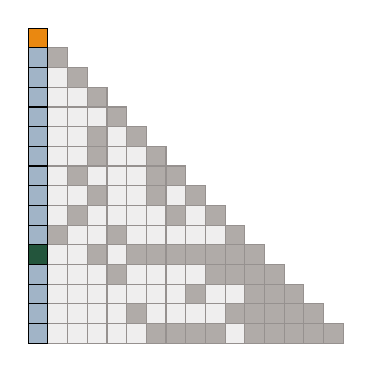
\begin{tikzpicture}[scale=4/16]
  \filldraw[draw=nnzborder, fill=nnzcolor] (1, -1) rectangle (2, -2);
  \filldraw[draw=zeroborder, fill=zerocolor] (1, -2) rectangle (2, -3);
  \filldraw[draw=zeroborder, fill=zerocolor] (1, -3) rectangle (2, -4);
  \filldraw[draw=zeroborder, fill=zerocolor] (1, -4) rectangle (2, -5);
  \filldraw[draw=zeroborder, fill=zerocolor] (1, -5) rectangle (2, -6);
  \filldraw[draw=zeroborder, fill=zerocolor] (1, -6) rectangle (2, -7);
  \filldraw[draw=zeroborder, fill=zerocolor] (1, -7) rectangle (2, -8);
  \filldraw[draw=zeroborder, fill=zerocolor] (1, -8) rectangle (2, -9);
  \filldraw[draw=zeroborder, fill=zerocolor] (1, -9) rectangle (2, -10);
  \filldraw[draw=nnzborder, fill=nnzcolor] (1, -10) rectangle (2, -11);
  \filldraw[draw=zeroborder, fill=zerocolor] (1, -11) rectangle (2, -12);
  \filldraw[draw=zeroborder, fill=zerocolor] (1, -12) rectangle (2, -13);
  \filldraw[draw=zeroborder, fill=zerocolor] (1, -13) rectangle (2, -14);
  \filldraw[draw=zeroborder, fill=zerocolor] (1, -14) rectangle (2, -15);
  \filldraw[draw=zeroborder, fill=zerocolor] (1, -15) rectangle (2, -16);
  \filldraw[draw=nnzborder, fill=nnzcolor] (2, -2) rectangle (3, -3);
  \filldraw[draw=zeroborder, fill=zerocolor] (2, -3) rectangle (3, -4);
  \filldraw[draw=zeroborder, fill=zerocolor] (2, -4) rectangle (3, -5);
  \filldraw[draw=zeroborder, fill=zerocolor] (2, -5) rectangle (3, -6);
  \filldraw[draw=zeroborder, fill=zerocolor] (2, -6) rectangle (3, -7);
  \filldraw[draw=nnzborder, fill=nnzcolor] (2, -7) rectangle (3, -8);
  \filldraw[draw=zeroborder, fill=zerocolor] (2, -8) rectangle (3, -9);
  \filldraw[draw=nnzborder, fill=nnzcolor] (2, -9) rectangle (3, -10);
  \filldraw[draw=zeroborder, fill=zerocolor] (2, -10) rectangle (3, -11);
  \filldraw[draw=zeroborder, fill=zerocolor] (2, -11) rectangle (3, -12);
  \filldraw[draw=zeroborder, fill=zerocolor] (2, -12) rectangle (3, -13);
  \filldraw[draw=zeroborder, fill=zerocolor] (2, -13) rectangle (3, -14);
  \filldraw[draw=zeroborder, fill=zerocolor] (2, -14) rectangle (3, -15);
  \filldraw[draw=zeroborder, fill=zerocolor] (2, -15) rectangle (3, -16);
  \filldraw[draw=nnzborder, fill=nnzcolor] (3, -3) rectangle (4, -4);
  \filldraw[draw=zeroborder, fill=zerocolor] (3, -4) rectangle (4, -5);
  \filldraw[draw=nnzborder, fill=nnzcolor] (3, -5) rectangle (4, -6);
  \filldraw[draw=nnzborder, fill=nnzcolor] (3, -6) rectangle (4, -7);
  \filldraw[draw=zeroborder, fill=zerocolor] (3, -7) rectangle (4, -8);
  \filldraw[draw=nnzborder, fill=nnzcolor] (3, -8) rectangle (4, -9);
  \filldraw[draw=zeroborder, fill=zerocolor] (3, -9) rectangle (4, -10);
  \filldraw[draw=zeroborder, fill=zerocolor] (3, -10) rectangle (4, -11);
  \filldraw[draw=nnzborder, fill=nnzcolor] (3, -11) rectangle (4, -12);
  \filldraw[draw=zeroborder, fill=zerocolor] (3, -12) rectangle (4, -13);
  \filldraw[draw=zeroborder, fill=zerocolor] (3, -13) rectangle (4, -14);
  \filldraw[draw=zeroborder, fill=zerocolor] (3, -14) rectangle (4, -15);
  \filldraw[draw=zeroborder, fill=zerocolor] (3, -15) rectangle (4, -16);
  \filldraw[draw=nnzborder, fill=nnzcolor] (4, -4) rectangle (5, -5);
  \filldraw[draw=zeroborder, fill=zerocolor] (4, -5) rectangle (5, -6);
  \filldraw[draw=zeroborder, fill=zerocolor] (4, -6) rectangle (5, -7);
  \filldraw[draw=zeroborder, fill=zerocolor] (4, -7) rectangle (5, -8);
  \filldraw[draw=zeroborder, fill=zerocolor] (4, -8) rectangle (5, -9);
  \filldraw[draw=zeroborder, fill=zerocolor] (4, -9) rectangle (5, -10);
  \filldraw[draw=nnzborder, fill=nnzcolor] (4, -10) rectangle (5, -11);
  \filldraw[draw=zeroborder, fill=zerocolor] (4, -11) rectangle (5, -12);
  \filldraw[draw=nnzborder, fill=nnzcolor] (4, -12) rectangle (5, -13);
  \filldraw[draw=zeroborder, fill=zerocolor] (4, -13) rectangle (5, -14);
  \filldraw[draw=zeroborder, fill=zerocolor] (4, -14) rectangle (5, -15);
  \filldraw[draw=zeroborder, fill=zerocolor] (4, -15) rectangle (5, -16);
  \filldraw[draw=nnzborder, fill=nnzcolor] (5, -5) rectangle (6, -6);
  \filldraw[draw=zeroborder, fill=zerocolor] (5, -6) rectangle (6, -7);
  \filldraw[draw=zeroborder, fill=zerocolor] (5, -7) rectangle (6, -8);
  \filldraw[draw=zeroborder, fill=zerocolor] (5, -8) rectangle (6, -9);
  \filldraw[draw=zeroborder, fill=zerocolor] (5, -9) rectangle (6, -10);
  \filldraw[draw=zeroborder, fill=zerocolor] (5, -10) rectangle (6, -11);
  \filldraw[draw=nnzborder, fill=nnzcolor] (5, -11) rectangle (6, -12);
  \filldraw[draw=zeroborder, fill=zerocolor] (5, -12) rectangle (6, -13);
  \filldraw[draw=zeroborder, fill=zerocolor] (5, -13) rectangle (6, -14);
  \filldraw[draw=nnzborder, fill=nnzcolor] (5, -14) rectangle (6, -15);
  \filldraw[draw=zeroborder, fill=zerocolor] (5, -15) rectangle (6, -16);
  \filldraw[draw=nnzborder, fill=nnzcolor] (6, -6) rectangle (7, -7);
  \filldraw[draw=nnzborder, fill=nnzcolor] (6, -7) rectangle (7, -8);
  \filldraw[draw=nnzborder, fill=nnzcolor] (6, -8) rectangle (7, -9);
  \filldraw[draw=zeroborder, fill=zerocolor] (6, -9) rectangle (7, -10);
  \filldraw[draw=zeroborder, fill=zerocolor] (6, -10) rectangle (7, -11);
  \filldraw[draw=nnzborder, fill=nnzcolor] (6, -11) rectangle (7, -12);
  \filldraw[draw=zeroborder, fill=zerocolor] (6, -12) rectangle (7, -13);
  \filldraw[draw=zeroborder, fill=zerocolor] (6, -13) rectangle (7, -14);
  \filldraw[draw=zeroborder, fill=zerocolor] (6, -14) rectangle (7, -15);
  \filldraw[draw=nnzborder, fill=nnzcolor] (6, -15) rectangle (7, -16);
  \filldraw[draw=nnzborder, fill=nnzcolor] (7, -7) rectangle (8, -8);
  \filldraw[draw=zeroborder, fill=zerocolor] (7, -8) rectangle (8, -9);
  \filldraw[draw=nnzborder, fill=nnzcolor] (7, -9) rectangle (8, -10);
  \filldraw[draw=zeroborder, fill=zerocolor] (7, -10) rectangle (8, -11);
  \filldraw[draw=nnzborder, fill=nnzcolor] (7, -11) rectangle (8, -12);
  \filldraw[draw=zeroborder, fill=zerocolor] (7, -12) rectangle (8, -13);
  \filldraw[draw=zeroborder, fill=zerocolor] (7, -13) rectangle (8, -14);
  \filldraw[draw=zeroborder, fill=zerocolor] (7, -14) rectangle (8, -15);
  \filldraw[draw=nnzborder, fill=nnzcolor] (7, -15) rectangle (8, -16);
  \filldraw[draw=nnzborder, fill=nnzcolor] (8, -8) rectangle (9, -9);
  \filldraw[draw=zeroborder, fill=zerocolor] (8, -9) rectangle (9, -10);
  \filldraw[draw=zeroborder, fill=zerocolor] (8, -10) rectangle (9, -11);
  \filldraw[draw=nnzborder, fill=nnzcolor] (8, -11) rectangle (9, -12);
  \filldraw[draw=zeroborder, fill=zerocolor] (8, -12) rectangle (9, -13);
  \filldraw[draw=nnzborder, fill=nnzcolor] (8, -13) rectangle (9, -14);
  \filldraw[draw=zeroborder, fill=zerocolor] (8, -14) rectangle (9, -15);
  \filldraw[draw=nnzborder, fill=nnzcolor] (8, -15) rectangle (9, -16);
  \filldraw[draw=nnzborder, fill=nnzcolor] (9, -9) rectangle (10, -10);
  \filldraw[draw=zeroborder, fill=zerocolor] (9, -10) rectangle (10, -11);
  \filldraw[draw=nnzborder, fill=nnzcolor] (9, -11) rectangle (10, -12);
  \filldraw[draw=nnzborder, fill=nnzcolor] (9, -12) rectangle (10, -13);
  \filldraw[draw=zeroborder, fill=zerocolor] (9, -13) rectangle (10, -14);
  \filldraw[draw=zeroborder, fill=zerocolor] (9, -14) rectangle (10, -15);
  \filldraw[draw=nnzborder, fill=nnzcolor] (9, -15) rectangle (10, -16);
  \filldraw[draw=nnzborder, fill=nnzcolor] (10, -10) rectangle (11, -11);
  \filldraw[draw=nnzborder, fill=nnzcolor] (10, -11) rectangle (11, -12);
  \filldraw[draw=nnzborder, fill=nnzcolor] (10, -12) rectangle (11, -13);
  \filldraw[draw=zeroborder, fill=zerocolor] (10, -13) rectangle (11, -14);
  \filldraw[draw=nnzborder, fill=nnzcolor] (10, -14) rectangle (11, -15);
  \filldraw[draw=zeroborder, fill=zerocolor] (10, -15) rectangle (11, -16);
  \filldraw[draw=nnzborder, fill=nnzcolor] (11, -11) rectangle (12, -12);
  \filldraw[draw=nnzborder, fill=nnzcolor] (11, -12) rectangle (12, -13);
  \filldraw[draw=nnzborder, fill=nnzcolor] (11, -13) rectangle (12, -14);
  \filldraw[draw=nnzborder, fill=nnzcolor] (11, -14) rectangle (12, -15);
  \filldraw[draw=nnzborder, fill=nnzcolor] (11, -15) rectangle (12, -16);
  \filldraw[draw=nnzborder, fill=nnzcolor] (12, -12) rectangle (13, -13);
  \filldraw[draw=nnzborder, fill=nnzcolor] (12, -13) rectangle (13, -14);
  \filldraw[draw=nnzborder, fill=nnzcolor] (12, -14) rectangle (13, -15);
  \filldraw[draw=nnzborder, fill=nnzcolor] (12, -15) rectangle (13, -16);
  \filldraw[draw=nnzborder, fill=nnzcolor] (13, -13) rectangle (14, -14);
  \filldraw[draw=nnzborder, fill=nnzcolor] (13, -14) rectangle (14, -15);
  \filldraw[draw=nnzborder, fill=nnzcolor] (13, -15) rectangle (14, -16);
  \filldraw[draw=nnzborder, fill=nnzcolor] (14, -14) rectangle (15, -15);
  \filldraw[draw=nnzborder, fill=nnzcolor] (14, -15) rectangle (15, -16);
  \filldraw[draw=nnzborder, fill=nnzcolor] (15, -15) rectangle (16, -16);
  \filldraw[draw=colborder, fill=targetcolor] (0, 0) rectangle (1, -1);
  \filldraw[draw=colborder, fill=candcolor] (0, -1) rectangle (1, -2);
  \filldraw[draw=colborder, fill=candcolor] (0, -2) rectangle (1, -3);
  \filldraw[draw=colborder, fill=candcolor] (0, -3) rectangle (1, -4);
  \filldraw[draw=colborder, fill=candcolor] (0, -4) rectangle (1, -5);
  \filldraw[draw=colborder, fill=candcolor] (0, -5) rectangle (1, -6);
  \filldraw[draw=colborder, fill=candcolor] (0, -6) rectangle (1, -7);
  \filldraw[draw=colborder, fill=candcolor] (0, -7) rectangle (1, -8);
  \filldraw[draw=colborder, fill=candcolor] (0, -8) rectangle (1, -9);
  \filldraw[draw=colborder, fill=candcolor] (0, -9) rectangle (1, -10);
  \filldraw[draw=colborder, fill=candcolor] (0, -10) rectangle (1, -11);
  \filldraw[draw=colborder, fill=selcolor] (0, -11) rectangle (1, -12);
  \filldraw[draw=colborder, fill=candcolor] (0, -12) rectangle (1, -13);
  \filldraw[draw=colborder, fill=candcolor] (0, -13) rectangle (1, -14);
  \filldraw[draw=colborder, fill=candcolor] (0, -14) rectangle (1, -15);
  \filldraw[draw=colborder, fill=candcolor] (0, -15) rectangle (1, -16);
\end{tikzpicture}
%
    \qquad
    \begin{tikzpicture}[baseline]
  \begin{axis}[
    % calculated from Cholesky factor, exactly 16 cm x 16 cm
    width={4cm},
    height={4cm},
    axis lines={none},
    % force axis box to have exactly the right dimensions, ignoring labels
    scale only axis=true,
  ]
  % consistent size bounding box
  \draw [white, line width=0] (-0.1, -0.1) -- (-0.1,  1.1);
  \draw [white, line width=0] ( 1.1, -0.1) -- ( 1.1,  1.1);
  \draw [white, line width=0] (-0.1, -0.1) -- (-1.1, -0.1);
  \draw [white, line width=0] (-0.1,  1.1) -- (-1.1,  1.1);
  \draw [seagreen!15, fill, radius=0.16075468063354492] (0.39122819049566204, 0.5167401826213637) circle;
  \draw [seagreen, radius=0.16075468063354492] (0.39122819049566204, 0.5167401826213637) circle;
  \draw [orange!25, fill, radius=0.08037734031677246] (0.39122819049566204, 0.5167401826213637) circle;
  \draw [orange, radius=0.08037734031677246] (0.39122819049566204, 0.5167401826213637) circle;
  \addplot [only marks, mark size=1, silver]    table
    {figures/points_knn/all_points.csv};
  \addplot [only marks, mark size=2, lightblue] table
    {figures/points_knn/candidates_16.csv};
  \addplot [only marks, mark size=4, seagreen]  table
    {figures/points_knn/selected_16.csv};
  \addplot [only marks, mark size=4, orange]    table
    {figures/points_knn/target_16.csv};
  \end{axis}
\end{tikzpicture}

  \end{figure}
}
\end{frame}

\section{Conditional selection}

\begin{frame}
\frametitle{This work: KL-minimization, revisited}
\framesubtitle{}

\begin{wideitemize}
  \item<+-> Plug optimal \( L \) back into the KL divergence
    \begin{align*}
      \KL*{\CM}{(L L^{\top})^{-1}} &=
        \sum_{i = 1}^N
          \left [
            \log \left ( \CM_{i, i \mid s_i \setminus \{ i \}} \right ) -
            \log \left ( \CM_{i, i \mid i + 1:} \right )
          \right ]
    \end{align*}
  \item<+-> KL \( \Leftrightarrow \) accumulated
    error over independent regression problems
  \item<+-> Goal: minimize posterior variance of \( i
    \)th prediction point by selecting training points
    \( s_i \) \emph{most informative} to that point
  \item<3->
    Variance \( \Leftrightarrow \) mutual information
    \( \Leftrightarrow \) mean squared error
\end{wideitemize}

\end{frame}

\begin{frame}
\frametitle{Conditional \( k \)-nearest neighbors}
\framesubtitle{}

% remove item indent just for this slide
% may want to consider removing indent all together since unnecessary
% but figures seem to be naturally indented
\setlength{\leftmargini}{0em}

% https://tex.stackexchange.com/questions/378548
\begin{minipage}[c][][c]{0.6\textwidth}
  \begin{wideitemize}
    \item<1-> Sparse Gaussian process regression,
      experimental design, active set, etc.
    \item<1-> Naive: select \( k \) closest points
    \item<2-> Chooses redundant information
    \item<3-> Maximize \emph{mutual information}!
  \end{wideitemize}
\end{minipage}%
\hfill
\begin{minipage}[c][][t]{0.4\textwidth}
  \begin{figure}[t!]
    \centering
    \only<1> {\begin{tikzpicture}[baseline]
  \begin{axis}[
    width={\linewidth},
    height={0.75\linewidth},
    axis lines={none},
    scale only axis={true},
    xmin=-1, xmax=1, ymin=-1.5, ymax=1.75,
  ]
  \addplot [only marks, mark size=2, lightblue]
    table {figures/selection/train.csv};
  \addplot [only marks, mark size=4, orange]
    table {figures/selection/test.csv};
  \addplot [only marks, mark size=4, seagreen]
    table {figures/selection/knn_selected_1.csv};
  \addplot [ultra thick, rust]
    table {figures/selection/knn_mean_1.csv};
  \addplot [name path=upper, forget plot, draw=none, rust]
    table {figures/selection/knn_std_upper_1.csv};
  \addplot [name path=lower, forget plot, draw=none, rust]
    table {figures/selection/knn_std_lower_1.csv};
  \addplot [rust!15] fill between [of=upper and lower];
\end{axis}
\end{tikzpicture}
}
    \only<2->{\begin{tikzpicture}[baseline]
  \begin{axis}[
    width={\linewidth},
    height={0.75\linewidth},
    axis lines={none},
    scale only axis={true},
    xmin=-1, xmax=1, ymin=-1.5, ymax=1.75,
  ]
  \addplot [only marks, mark size=2, lightblue]
    table {figures/selection/train.csv};
  \addplot [only marks, mark size=4, orange]
    table {figures/selection/test.csv};
  \addplot [only marks, mark size=4, seagreen]
    table {figures/selection/knn_selected_2.csv};
  \addplot [ultra thick, rust]
    table {figures/selection/knn_mean_2.csv};
  \addplot [name path=upper, forget plot, draw=none, rust]
    table {figures/selection/knn_std_upper_2.csv};
  \addplot [name path=lower, forget plot, draw=none, rust]
    table {figures/selection/knn_std_lower_2.csv};
  \addplot [rust!15] fill between [of=upper and lower];
\end{axis}
\end{tikzpicture}
}
  \end{figure}
  \vspace{-5\baselineskip}
  \uncover<3-> {
    \begin{figure}
      \centering
      \only<-3>{\begin{tikzpicture}[baseline]
  \begin{axis}[
    width={\linewidth},
    height={0.75\linewidth},
    axis lines={none},
    scale only axis={true},
    xmin=-1, xmax=1, ymin=-1.5, ymax=1.75,
  ]
  \addplot [only marks, mark size=2, lightblue]
    table {figures/selection/train.csv};
  \addplot [only marks, mark size=4, orange]
    table {figures/selection/test.csv};
  \addplot [only marks, mark size=4, seagreen]
    table {figures/selection/cknn_selected_1.csv};
  \addplot [ultra thick, rust]
    table {figures/selection/cknn_mean_1.csv};
  \addplot [name path=upper, forget plot, draw=none, rust]
    table {figures/selection/cknn_std_upper_1.csv};
  \addplot [name path=lower, forget plot, draw=none, rust]
    table {figures/selection/cknn_std_lower_1.csv};
  \addplot [rust!15] fill between [of=upper and lower];
\end{axis}
\end{tikzpicture}
}
      \only<4->{\begin{tikzpicture}[baseline]
  \begin{axis}[
    width={\linewidth},
    height={0.75\linewidth},
    axis lines={none},
    scale only axis={true},
    xmin=-1, xmax=1, ymin=-1.5, ymax=1.75,
  ]
  \addplot [only marks, mark size=2, lightblue]
    table {figures/selection/train.csv};
  \addplot [only marks, mark size=4, orange]
    table {figures/selection/test.csv};
  \addplot [only marks, mark size=4, seagreen]
    table {figures/selection/cknn_selected_2.csv};
  \addplot [ultra thick, rust]
    table {figures/selection/cknn_mean_2.csv};
  \addplot [name path=upper, forget plot, draw=none, rust]
    table {figures/selection/cknn_std_upper_2.csv};
  \addplot [name path=lower, forget plot, draw=none, rust]
    table {figures/selection/cknn_std_lower_2.csv};
  \addplot [rust!15] fill between [of=upper and lower];
\end{axis}
\end{tikzpicture}
}
    \end{figure}
  }
\end{minipage}
\end{frame}

\begin{frame}
\frametitle{Cholesky factorization by greedy selection}
\framesubtitle{}

\begin{wideitemize}
  \item Identify \textcolor{orange}{target} point as the
    \textcolor{orange}{diagonal entry}, \textcolor{lightblue}{candidates} are
    \textcolor{lightblue}{below} it, and add \textcolor{seagreen}{selected
    entries} to the \textcolor{seagreen}{sparsity pattern}
  \item In practice, restrict candidate set to nearest neighbors, e.g.
\end{wideitemize}

% computer generated
\only<1>{
  \begin{figure}
    \centering
    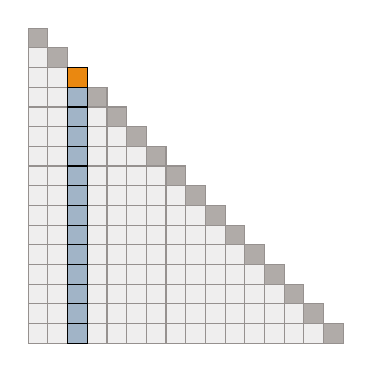
\begin{tikzpicture}[scale=4/16]
  \filldraw[draw=nnzborder, fill=nnzcolor] (0, 0) rectangle (1, -1);
  \filldraw[draw=zeroborder, fill=zerocolor] (0, -1) rectangle (1, -2);
  \filldraw[draw=zeroborder, fill=zerocolor] (0, -2) rectangle (1, -3);
  \filldraw[draw=zeroborder, fill=zerocolor] (0, -3) rectangle (1, -4);
  \filldraw[draw=zeroborder, fill=zerocolor] (0, -4) rectangle (1, -5);
  \filldraw[draw=zeroborder, fill=zerocolor] (0, -5) rectangle (1, -6);
  \filldraw[draw=zeroborder, fill=zerocolor] (0, -6) rectangle (1, -7);
  \filldraw[draw=zeroborder, fill=zerocolor] (0, -7) rectangle (1, -8);
  \filldraw[draw=zeroborder, fill=zerocolor] (0, -8) rectangle (1, -9);
  \filldraw[draw=zeroborder, fill=zerocolor] (0, -9) rectangle (1, -10);
  \filldraw[draw=zeroborder, fill=zerocolor] (0, -10) rectangle (1, -11);
  \filldraw[draw=zeroborder, fill=zerocolor] (0, -11) rectangle (1, -12);
  \filldraw[draw=zeroborder, fill=zerocolor] (0, -12) rectangle (1, -13);
  \filldraw[draw=zeroborder, fill=zerocolor] (0, -13) rectangle (1, -14);
  \filldraw[draw=zeroborder, fill=zerocolor] (0, -14) rectangle (1, -15);
  \filldraw[draw=zeroborder, fill=zerocolor] (0, -15) rectangle (1, -16);
  \filldraw[draw=nnzborder, fill=nnzcolor] (1, -1) rectangle (2, -2);
  \filldraw[draw=zeroborder, fill=zerocolor] (1, -2) rectangle (2, -3);
  \filldraw[draw=zeroborder, fill=zerocolor] (1, -3) rectangle (2, -4);
  \filldraw[draw=zeroborder, fill=zerocolor] (1, -4) rectangle (2, -5);
  \filldraw[draw=zeroborder, fill=zerocolor] (1, -5) rectangle (2, -6);
  \filldraw[draw=zeroborder, fill=zerocolor] (1, -6) rectangle (2, -7);
  \filldraw[draw=zeroborder, fill=zerocolor] (1, -7) rectangle (2, -8);
  \filldraw[draw=zeroborder, fill=zerocolor] (1, -8) rectangle (2, -9);
  \filldraw[draw=zeroborder, fill=zerocolor] (1, -9) rectangle (2, -10);
  \filldraw[draw=zeroborder, fill=zerocolor] (1, -10) rectangle (2, -11);
  \filldraw[draw=zeroborder, fill=zerocolor] (1, -11) rectangle (2, -12);
  \filldraw[draw=zeroborder, fill=zerocolor] (1, -12) rectangle (2, -13);
  \filldraw[draw=zeroborder, fill=zerocolor] (1, -13) rectangle (2, -14);
  \filldraw[draw=zeroborder, fill=zerocolor] (1, -14) rectangle (2, -15);
  \filldraw[draw=zeroborder, fill=zerocolor] (1, -15) rectangle (2, -16);
  \filldraw[draw=nnzborder, fill=nnzcolor] (3, -3) rectangle (4, -4);
  \filldraw[draw=zeroborder, fill=zerocolor] (3, -4) rectangle (4, -5);
  \filldraw[draw=zeroborder, fill=zerocolor] (3, -5) rectangle (4, -6);
  \filldraw[draw=zeroborder, fill=zerocolor] (3, -6) rectangle (4, -7);
  \filldraw[draw=zeroborder, fill=zerocolor] (3, -7) rectangle (4, -8);
  \filldraw[draw=zeroborder, fill=zerocolor] (3, -8) rectangle (4, -9);
  \filldraw[draw=zeroborder, fill=zerocolor] (3, -9) rectangle (4, -10);
  \filldraw[draw=zeroborder, fill=zerocolor] (3, -10) rectangle (4, -11);
  \filldraw[draw=zeroborder, fill=zerocolor] (3, -11) rectangle (4, -12);
  \filldraw[draw=zeroborder, fill=zerocolor] (3, -12) rectangle (4, -13);
  \filldraw[draw=zeroborder, fill=zerocolor] (3, -13) rectangle (4, -14);
  \filldraw[draw=zeroborder, fill=zerocolor] (3, -14) rectangle (4, -15);
  \filldraw[draw=zeroborder, fill=zerocolor] (3, -15) rectangle (4, -16);
  \filldraw[draw=nnzborder, fill=nnzcolor] (4, -4) rectangle (5, -5);
  \filldraw[draw=zeroborder, fill=zerocolor] (4, -5) rectangle (5, -6);
  \filldraw[draw=zeroborder, fill=zerocolor] (4, -6) rectangle (5, -7);
  \filldraw[draw=zeroborder, fill=zerocolor] (4, -7) rectangle (5, -8);
  \filldraw[draw=zeroborder, fill=zerocolor] (4, -8) rectangle (5, -9);
  \filldraw[draw=zeroborder, fill=zerocolor] (4, -9) rectangle (5, -10);
  \filldraw[draw=zeroborder, fill=zerocolor] (4, -10) rectangle (5, -11);
  \filldraw[draw=zeroborder, fill=zerocolor] (4, -11) rectangle (5, -12);
  \filldraw[draw=zeroborder, fill=zerocolor] (4, -12) rectangle (5, -13);
  \filldraw[draw=zeroborder, fill=zerocolor] (4, -13) rectangle (5, -14);
  \filldraw[draw=zeroborder, fill=zerocolor] (4, -14) rectangle (5, -15);
  \filldraw[draw=zeroborder, fill=zerocolor] (4, -15) rectangle (5, -16);
  \filldraw[draw=nnzborder, fill=nnzcolor] (5, -5) rectangle (6, -6);
  \filldraw[draw=zeroborder, fill=zerocolor] (5, -6) rectangle (6, -7);
  \filldraw[draw=zeroborder, fill=zerocolor] (5, -7) rectangle (6, -8);
  \filldraw[draw=zeroborder, fill=zerocolor] (5, -8) rectangle (6, -9);
  \filldraw[draw=zeroborder, fill=zerocolor] (5, -9) rectangle (6, -10);
  \filldraw[draw=zeroborder, fill=zerocolor] (5, -10) rectangle (6, -11);
  \filldraw[draw=zeroborder, fill=zerocolor] (5, -11) rectangle (6, -12);
  \filldraw[draw=zeroborder, fill=zerocolor] (5, -12) rectangle (6, -13);
  \filldraw[draw=zeroborder, fill=zerocolor] (5, -13) rectangle (6, -14);
  \filldraw[draw=zeroborder, fill=zerocolor] (5, -14) rectangle (6, -15);
  \filldraw[draw=zeroborder, fill=zerocolor] (5, -15) rectangle (6, -16);
  \filldraw[draw=nnzborder, fill=nnzcolor] (6, -6) rectangle (7, -7);
  \filldraw[draw=zeroborder, fill=zerocolor] (6, -7) rectangle (7, -8);
  \filldraw[draw=zeroborder, fill=zerocolor] (6, -8) rectangle (7, -9);
  \filldraw[draw=zeroborder, fill=zerocolor] (6, -9) rectangle (7, -10);
  \filldraw[draw=zeroborder, fill=zerocolor] (6, -10) rectangle (7, -11);
  \filldraw[draw=zeroborder, fill=zerocolor] (6, -11) rectangle (7, -12);
  \filldraw[draw=zeroborder, fill=zerocolor] (6, -12) rectangle (7, -13);
  \filldraw[draw=zeroborder, fill=zerocolor] (6, -13) rectangle (7, -14);
  \filldraw[draw=zeroborder, fill=zerocolor] (6, -14) rectangle (7, -15);
  \filldraw[draw=zeroborder, fill=zerocolor] (6, -15) rectangle (7, -16);
  \filldraw[draw=nnzborder, fill=nnzcolor] (7, -7) rectangle (8, -8);
  \filldraw[draw=zeroborder, fill=zerocolor] (7, -8) rectangle (8, -9);
  \filldraw[draw=zeroborder, fill=zerocolor] (7, -9) rectangle (8, -10);
  \filldraw[draw=zeroborder, fill=zerocolor] (7, -10) rectangle (8, -11);
  \filldraw[draw=zeroborder, fill=zerocolor] (7, -11) rectangle (8, -12);
  \filldraw[draw=zeroborder, fill=zerocolor] (7, -12) rectangle (8, -13);
  \filldraw[draw=zeroborder, fill=zerocolor] (7, -13) rectangle (8, -14);
  \filldraw[draw=zeroborder, fill=zerocolor] (7, -14) rectangle (8, -15);
  \filldraw[draw=zeroborder, fill=zerocolor] (7, -15) rectangle (8, -16);
  \filldraw[draw=nnzborder, fill=nnzcolor] (8, -8) rectangle (9, -9);
  \filldraw[draw=zeroborder, fill=zerocolor] (8, -9) rectangle (9, -10);
  \filldraw[draw=zeroborder, fill=zerocolor] (8, -10) rectangle (9, -11);
  \filldraw[draw=zeroborder, fill=zerocolor] (8, -11) rectangle (9, -12);
  \filldraw[draw=zeroborder, fill=zerocolor] (8, -12) rectangle (9, -13);
  \filldraw[draw=zeroborder, fill=zerocolor] (8, -13) rectangle (9, -14);
  \filldraw[draw=zeroborder, fill=zerocolor] (8, -14) rectangle (9, -15);
  \filldraw[draw=zeroborder, fill=zerocolor] (8, -15) rectangle (9, -16);
  \filldraw[draw=nnzborder, fill=nnzcolor] (9, -9) rectangle (10, -10);
  \filldraw[draw=zeroborder, fill=zerocolor] (9, -10) rectangle (10, -11);
  \filldraw[draw=zeroborder, fill=zerocolor] (9, -11) rectangle (10, -12);
  \filldraw[draw=zeroborder, fill=zerocolor] (9, -12) rectangle (10, -13);
  \filldraw[draw=zeroborder, fill=zerocolor] (9, -13) rectangle (10, -14);
  \filldraw[draw=zeroborder, fill=zerocolor] (9, -14) rectangle (10, -15);
  \filldraw[draw=zeroborder, fill=zerocolor] (9, -15) rectangle (10, -16);
  \filldraw[draw=nnzborder, fill=nnzcolor] (10, -10) rectangle (11, -11);
  \filldraw[draw=zeroborder, fill=zerocolor] (10, -11) rectangle (11, -12);
  \filldraw[draw=zeroborder, fill=zerocolor] (10, -12) rectangle (11, -13);
  \filldraw[draw=zeroborder, fill=zerocolor] (10, -13) rectangle (11, -14);
  \filldraw[draw=zeroborder, fill=zerocolor] (10, -14) rectangle (11, -15);
  \filldraw[draw=zeroborder, fill=zerocolor] (10, -15) rectangle (11, -16);
  \filldraw[draw=nnzborder, fill=nnzcolor] (11, -11) rectangle (12, -12);
  \filldraw[draw=zeroborder, fill=zerocolor] (11, -12) rectangle (12, -13);
  \filldraw[draw=zeroborder, fill=zerocolor] (11, -13) rectangle (12, -14);
  \filldraw[draw=zeroborder, fill=zerocolor] (11, -14) rectangle (12, -15);
  \filldraw[draw=zeroborder, fill=zerocolor] (11, -15) rectangle (12, -16);
  \filldraw[draw=nnzborder, fill=nnzcolor] (12, -12) rectangle (13, -13);
  \filldraw[draw=zeroborder, fill=zerocolor] (12, -13) rectangle (13, -14);
  \filldraw[draw=zeroborder, fill=zerocolor] (12, -14) rectangle (13, -15);
  \filldraw[draw=zeroborder, fill=zerocolor] (12, -15) rectangle (13, -16);
  \filldraw[draw=nnzborder, fill=nnzcolor] (13, -13) rectangle (14, -14);
  \filldraw[draw=zeroborder, fill=zerocolor] (13, -14) rectangle (14, -15);
  \filldraw[draw=zeroborder, fill=zerocolor] (13, -15) rectangle (14, -16);
  \filldraw[draw=nnzborder, fill=nnzcolor] (14, -14) rectangle (15, -15);
  \filldraw[draw=zeroborder, fill=zerocolor] (14, -15) rectangle (15, -16);
  \filldraw[draw=nnzborder, fill=nnzcolor] (15, -15) rectangle (16, -16);
  \filldraw[draw=colborder, fill=targetcolor] (2, -2) rectangle (3, -3);
  \filldraw[draw=colborder, fill=candcolor] (2, -3) rectangle (3, -4);
  \filldraw[draw=colborder, fill=candcolor] (2, -4) rectangle (3, -5);
  \filldraw[draw=colborder, fill=candcolor] (2, -5) rectangle (3, -6);
  \filldraw[draw=colborder, fill=candcolor] (2, -6) rectangle (3, -7);
  \filldraw[draw=colborder, fill=candcolor] (2, -7) rectangle (3, -8);
  \filldraw[draw=colborder, fill=candcolor] (2, -8) rectangle (3, -9);
  \filldraw[draw=colborder, fill=candcolor] (2, -9) rectangle (3, -10);
  \filldraw[draw=colborder, fill=candcolor] (2, -10) rectangle (3, -11);
  \filldraw[draw=colborder, fill=candcolor] (2, -11) rectangle (3, -12);
  \filldraw[draw=colborder, fill=candcolor] (2, -12) rectangle (3, -13);
  \filldraw[draw=colborder, fill=candcolor] (2, -13) rectangle (3, -14);
  \filldraw[draw=colborder, fill=candcolor] (2, -14) rectangle (3, -15);
  \filldraw[draw=colborder, fill=candcolor] (2, -15) rectangle (3, -16);
\end{tikzpicture}
%
    \qquad
    \begin{tikzpicture}[baseline]
  \begin{axis}[
    % calculated from Cholesky factor, exactly 16 cm x 16 cm
    width={4cm},
    height={4cm},
    axis lines={none},
    % force axis box to have exactly the right dimensions, ignoring labels
    scale only axis=true,
  ]
  % consistent size bounding box
  \draw [white, line width=0] (-0.1, -0.1) -- (-0.1,  1.1);
  \draw [white, line width=0] ( 1.1, -0.1) -- ( 1.1,  1.1);
  \draw [white, line width=0] (-0.1, -0.1) -- (-1.1, -0.1);
  \draw [white, line width=0] (-0.1,  1.1) -- (-1.1,  1.1);
  \draw [seagreen!15, fill, radius=4.0] (0.08564916714362436, 0.2368105065960997) circle;
  \draw [seagreen, radius=4.0] (0.08564916714362436, 0.2368105065960997) circle;
  \draw [orange!25, fill, radius=2.0] (0.08564916714362436, 0.2368105065960997) circle;
  \draw [orange, radius=2.0] (0.08564916714362436, 0.2368105065960997) circle;
  \addplot [only marks, mark size=1, silver]    table
    {figures/points_knn/all_points.csv};
  \addplot [only marks, mark size=2, lightblue] table
    {figures/points_knn/candidates_01.csv};
  \addplot [only marks, mark size=4, seagreen]  table
    {figures/points_knn/selected_01.csv};
  \addplot [only marks, mark size=4, orange]    table
    {figures/points_knn/target_01.csv};
  \end{axis}
\end{tikzpicture}

  \end{figure}
}
\only<2>{
  \begin{figure}
    \centering
    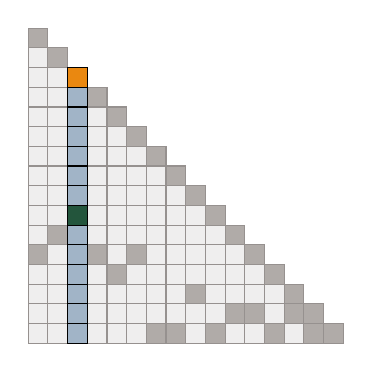
\begin{tikzpicture}[scale=4/16]
  \filldraw[draw=nnzborder, fill=nnzcolor] (0, 0) rectangle (1, -1);
  \filldraw[draw=zeroborder, fill=zerocolor] (0, -1) rectangle (1, -2);
  \filldraw[draw=zeroborder, fill=zerocolor] (0, -2) rectangle (1, -3);
  \filldraw[draw=zeroborder, fill=zerocolor] (0, -3) rectangle (1, -4);
  \filldraw[draw=zeroborder, fill=zerocolor] (0, -4) rectangle (1, -5);
  \filldraw[draw=zeroborder, fill=zerocolor] (0, -5) rectangle (1, -6);
  \filldraw[draw=zeroborder, fill=zerocolor] (0, -6) rectangle (1, -7);
  \filldraw[draw=zeroborder, fill=zerocolor] (0, -7) rectangle (1, -8);
  \filldraw[draw=zeroborder, fill=zerocolor] (0, -8) rectangle (1, -9);
  \filldraw[draw=zeroborder, fill=zerocolor] (0, -9) rectangle (1, -10);
  \filldraw[draw=zeroborder, fill=zerocolor] (0, -10) rectangle (1, -11);
  \filldraw[draw=nnzborder, fill=nnzcolor] (0, -11) rectangle (1, -12);
  \filldraw[draw=zeroborder, fill=zerocolor] (0, -12) rectangle (1, -13);
  \filldraw[draw=zeroborder, fill=zerocolor] (0, -13) rectangle (1, -14);
  \filldraw[draw=zeroborder, fill=zerocolor] (0, -14) rectangle (1, -15);
  \filldraw[draw=zeroborder, fill=zerocolor] (0, -15) rectangle (1, -16);
  \filldraw[draw=nnzborder, fill=nnzcolor] (1, -1) rectangle (2, -2);
  \filldraw[draw=zeroborder, fill=zerocolor] (1, -2) rectangle (2, -3);
  \filldraw[draw=zeroborder, fill=zerocolor] (1, -3) rectangle (2, -4);
  \filldraw[draw=zeroborder, fill=zerocolor] (1, -4) rectangle (2, -5);
  \filldraw[draw=zeroborder, fill=zerocolor] (1, -5) rectangle (2, -6);
  \filldraw[draw=zeroborder, fill=zerocolor] (1, -6) rectangle (2, -7);
  \filldraw[draw=zeroborder, fill=zerocolor] (1, -7) rectangle (2, -8);
  \filldraw[draw=zeroborder, fill=zerocolor] (1, -8) rectangle (2, -9);
  \filldraw[draw=zeroborder, fill=zerocolor] (1, -9) rectangle (2, -10);
  \filldraw[draw=nnzborder, fill=nnzcolor] (1, -10) rectangle (2, -11);
  \filldraw[draw=zeroborder, fill=zerocolor] (1, -11) rectangle (2, -12);
  \filldraw[draw=zeroborder, fill=zerocolor] (1, -12) rectangle (2, -13);
  \filldraw[draw=zeroborder, fill=zerocolor] (1, -13) rectangle (2, -14);
  \filldraw[draw=zeroborder, fill=zerocolor] (1, -14) rectangle (2, -15);
  \filldraw[draw=zeroborder, fill=zerocolor] (1, -15) rectangle (2, -16);
  \filldraw[draw=nnzborder, fill=nnzcolor] (3, -3) rectangle (4, -4);
  \filldraw[draw=zeroborder, fill=zerocolor] (3, -4) rectangle (4, -5);
  \filldraw[draw=zeroborder, fill=zerocolor] (3, -5) rectangle (4, -6);
  \filldraw[draw=zeroborder, fill=zerocolor] (3, -6) rectangle (4, -7);
  \filldraw[draw=zeroborder, fill=zerocolor] (3, -7) rectangle (4, -8);
  \filldraw[draw=zeroborder, fill=zerocolor] (3, -8) rectangle (4, -9);
  \filldraw[draw=zeroborder, fill=zerocolor] (3, -9) rectangle (4, -10);
  \filldraw[draw=zeroborder, fill=zerocolor] (3, -10) rectangle (4, -11);
  \filldraw[draw=nnzborder, fill=nnzcolor] (3, -11) rectangle (4, -12);
  \filldraw[draw=zeroborder, fill=zerocolor] (3, -12) rectangle (4, -13);
  \filldraw[draw=zeroborder, fill=zerocolor] (3, -13) rectangle (4, -14);
  \filldraw[draw=zeroborder, fill=zerocolor] (3, -14) rectangle (4, -15);
  \filldraw[draw=zeroborder, fill=zerocolor] (3, -15) rectangle (4, -16);
  \filldraw[draw=nnzborder, fill=nnzcolor] (4, -4) rectangle (5, -5);
  \filldraw[draw=zeroborder, fill=zerocolor] (4, -5) rectangle (5, -6);
  \filldraw[draw=zeroborder, fill=zerocolor] (4, -6) rectangle (5, -7);
  \filldraw[draw=zeroborder, fill=zerocolor] (4, -7) rectangle (5, -8);
  \filldraw[draw=zeroborder, fill=zerocolor] (4, -8) rectangle (5, -9);
  \filldraw[draw=zeroborder, fill=zerocolor] (4, -9) rectangle (5, -10);
  \filldraw[draw=zeroborder, fill=zerocolor] (4, -10) rectangle (5, -11);
  \filldraw[draw=zeroborder, fill=zerocolor] (4, -11) rectangle (5, -12);
  \filldraw[draw=nnzborder, fill=nnzcolor] (4, -12) rectangle (5, -13);
  \filldraw[draw=zeroborder, fill=zerocolor] (4, -13) rectangle (5, -14);
  \filldraw[draw=zeroborder, fill=zerocolor] (4, -14) rectangle (5, -15);
  \filldraw[draw=zeroborder, fill=zerocolor] (4, -15) rectangle (5, -16);
  \filldraw[draw=nnzborder, fill=nnzcolor] (5, -5) rectangle (6, -6);
  \filldraw[draw=zeroborder, fill=zerocolor] (5, -6) rectangle (6, -7);
  \filldraw[draw=zeroborder, fill=zerocolor] (5, -7) rectangle (6, -8);
  \filldraw[draw=zeroborder, fill=zerocolor] (5, -8) rectangle (6, -9);
  \filldraw[draw=zeroborder, fill=zerocolor] (5, -9) rectangle (6, -10);
  \filldraw[draw=zeroborder, fill=zerocolor] (5, -10) rectangle (6, -11);
  \filldraw[draw=nnzborder, fill=nnzcolor] (5, -11) rectangle (6, -12);
  \filldraw[draw=zeroborder, fill=zerocolor] (5, -12) rectangle (6, -13);
  \filldraw[draw=zeroborder, fill=zerocolor] (5, -13) rectangle (6, -14);
  \filldraw[draw=zeroborder, fill=zerocolor] (5, -14) rectangle (6, -15);
  \filldraw[draw=zeroborder, fill=zerocolor] (5, -15) rectangle (6, -16);
  \filldraw[draw=nnzborder, fill=nnzcolor] (6, -6) rectangle (7, -7);
  \filldraw[draw=zeroborder, fill=zerocolor] (6, -7) rectangle (7, -8);
  \filldraw[draw=zeroborder, fill=zerocolor] (6, -8) rectangle (7, -9);
  \filldraw[draw=zeroborder, fill=zerocolor] (6, -9) rectangle (7, -10);
  \filldraw[draw=zeroborder, fill=zerocolor] (6, -10) rectangle (7, -11);
  \filldraw[draw=zeroborder, fill=zerocolor] (6, -11) rectangle (7, -12);
  \filldraw[draw=zeroborder, fill=zerocolor] (6, -12) rectangle (7, -13);
  \filldraw[draw=zeroborder, fill=zerocolor] (6, -13) rectangle (7, -14);
  \filldraw[draw=zeroborder, fill=zerocolor] (6, -14) rectangle (7, -15);
  \filldraw[draw=nnzborder, fill=nnzcolor] (6, -15) rectangle (7, -16);
  \filldraw[draw=nnzborder, fill=nnzcolor] (7, -7) rectangle (8, -8);
  \filldraw[draw=zeroborder, fill=zerocolor] (7, -8) rectangle (8, -9);
  \filldraw[draw=zeroborder, fill=zerocolor] (7, -9) rectangle (8, -10);
  \filldraw[draw=zeroborder, fill=zerocolor] (7, -10) rectangle (8, -11);
  \filldraw[draw=zeroborder, fill=zerocolor] (7, -11) rectangle (8, -12);
  \filldraw[draw=zeroborder, fill=zerocolor] (7, -12) rectangle (8, -13);
  \filldraw[draw=zeroborder, fill=zerocolor] (7, -13) rectangle (8, -14);
  \filldraw[draw=zeroborder, fill=zerocolor] (7, -14) rectangle (8, -15);
  \filldraw[draw=nnzborder, fill=nnzcolor] (7, -15) rectangle (8, -16);
  \filldraw[draw=nnzborder, fill=nnzcolor] (8, -8) rectangle (9, -9);
  \filldraw[draw=zeroborder, fill=zerocolor] (8, -9) rectangle (9, -10);
  \filldraw[draw=zeroborder, fill=zerocolor] (8, -10) rectangle (9, -11);
  \filldraw[draw=zeroborder, fill=zerocolor] (8, -11) rectangle (9, -12);
  \filldraw[draw=zeroborder, fill=zerocolor] (8, -12) rectangle (9, -13);
  \filldraw[draw=nnzborder, fill=nnzcolor] (8, -13) rectangle (9, -14);
  \filldraw[draw=zeroborder, fill=zerocolor] (8, -14) rectangle (9, -15);
  \filldraw[draw=zeroborder, fill=zerocolor] (8, -15) rectangle (9, -16);
  \filldraw[draw=nnzborder, fill=nnzcolor] (9, -9) rectangle (10, -10);
  \filldraw[draw=zeroborder, fill=zerocolor] (9, -10) rectangle (10, -11);
  \filldraw[draw=zeroborder, fill=zerocolor] (9, -11) rectangle (10, -12);
  \filldraw[draw=zeroborder, fill=zerocolor] (9, -12) rectangle (10, -13);
  \filldraw[draw=zeroborder, fill=zerocolor] (9, -13) rectangle (10, -14);
  \filldraw[draw=zeroborder, fill=zerocolor] (9, -14) rectangle (10, -15);
  \filldraw[draw=nnzborder, fill=nnzcolor] (9, -15) rectangle (10, -16);
  \filldraw[draw=nnzborder, fill=nnzcolor] (10, -10) rectangle (11, -11);
  \filldraw[draw=zeroborder, fill=zerocolor] (10, -11) rectangle (11, -12);
  \filldraw[draw=zeroborder, fill=zerocolor] (10, -12) rectangle (11, -13);
  \filldraw[draw=zeroborder, fill=zerocolor] (10, -13) rectangle (11, -14);
  \filldraw[draw=nnzborder, fill=nnzcolor] (10, -14) rectangle (11, -15);
  \filldraw[draw=zeroborder, fill=zerocolor] (10, -15) rectangle (11, -16);
  \filldraw[draw=nnzborder, fill=nnzcolor] (11, -11) rectangle (12, -12);
  \filldraw[draw=zeroborder, fill=zerocolor] (11, -12) rectangle (12, -13);
  \filldraw[draw=zeroborder, fill=zerocolor] (11, -13) rectangle (12, -14);
  \filldraw[draw=nnzborder, fill=nnzcolor] (11, -14) rectangle (12, -15);
  \filldraw[draw=zeroborder, fill=zerocolor] (11, -15) rectangle (12, -16);
  \filldraw[draw=nnzborder, fill=nnzcolor] (12, -12) rectangle (13, -13);
  \filldraw[draw=zeroborder, fill=zerocolor] (12, -13) rectangle (13, -14);
  \filldraw[draw=zeroborder, fill=zerocolor] (12, -14) rectangle (13, -15);
  \filldraw[draw=nnzborder, fill=nnzcolor] (12, -15) rectangle (13, -16);
  \filldraw[draw=nnzborder, fill=nnzcolor] (13, -13) rectangle (14, -14);
  \filldraw[draw=nnzborder, fill=nnzcolor] (13, -14) rectangle (14, -15);
  \filldraw[draw=zeroborder, fill=zerocolor] (13, -15) rectangle (14, -16);
  \filldraw[draw=nnzborder, fill=nnzcolor] (14, -14) rectangle (15, -15);
  \filldraw[draw=nnzborder, fill=nnzcolor] (14, -15) rectangle (15, -16);
  \filldraw[draw=nnzborder, fill=nnzcolor] (15, -15) rectangle (16, -16);
  \filldraw[draw=colborder, fill=targetcolor] (2, -2) rectangle (3, -3);
  \filldraw[draw=colborder, fill=candcolor] (2, -3) rectangle (3, -4);
  \filldraw[draw=colborder, fill=candcolor] (2, -4) rectangle (3, -5);
  \filldraw[draw=colborder, fill=candcolor] (2, -5) rectangle (3, -6);
  \filldraw[draw=colborder, fill=candcolor] (2, -6) rectangle (3, -7);
  \filldraw[draw=colborder, fill=candcolor] (2, -7) rectangle (3, -8);
  \filldraw[draw=colborder, fill=candcolor] (2, -8) rectangle (3, -9);
  \filldraw[draw=colborder, fill=selcolor] (2, -9) rectangle (3, -10);
  \filldraw[draw=colborder, fill=candcolor] (2, -10) rectangle (3, -11);
  \filldraw[draw=colborder, fill=candcolor] (2, -11) rectangle (3, -12);
  \filldraw[draw=colborder, fill=candcolor] (2, -12) rectangle (3, -13);
  \filldraw[draw=colborder, fill=candcolor] (2, -13) rectangle (3, -14);
  \filldraw[draw=colborder, fill=candcolor] (2, -14) rectangle (3, -15);
  \filldraw[draw=colborder, fill=candcolor] (2, -15) rectangle (3, -16);
\end{tikzpicture}
%
    \qquad
    \begin{tikzpicture}[baseline]
  \begin{axis}[
    % calculated from Cholesky factor, exactly 16 cm x 16 cm
    width={4cm},
    height={4cm},
    axis lines={none},
    % force axis box to have exactly the right dimensions, ignoring labels
    scale only axis=true,
  ]
  % consistent size bounding box
  \draw [white, line width=0] (-0.1, -0.1) -- (-0.1,  1.1);
  \draw [white, line width=0] ( 1.1, -0.1) -- ( 1.1,  1.1);
  \draw [white, line width=0] (-0.1, -0.1) -- (-1.1, -0.1);
  \draw [white, line width=0] (-0.1,  1.1) -- (-1.1,  1.1);
  \draw [seagreen!15, fill, radius=1.9421300888061523] (0.7378377872921602, 0.9562672548360985) circle;
  \draw [seagreen, radius=1.9421300888061523] (0.7378377872921602, 0.9562672548360985) circle;
  \draw [orange!25, fill, radius=0.9710650444030762] (0.7378377872921602, 0.9562672548360985) circle;
  \draw [orange, radius=0.9710650444030762] (0.7378377872921602, 0.9562672548360985) circle;
  \addplot [only marks, mark size=1, silver]    table
    {figures/points_knn/all_points.csv};
  \addplot [only marks, mark size=2, lightblue] table
    {figures/points_knn/candidates_02.csv};
  \addplot [only marks, mark size=4, seagreen]  table
    {figures/points_knn/selected_02.csv};
  \addplot [only marks, mark size=4, orange]    table
    {figures/points_knn/target_02.csv};
  \end{axis}
\end{tikzpicture}

  \end{figure}
}
\only<3>{
  \begin{figure}
    \centering
    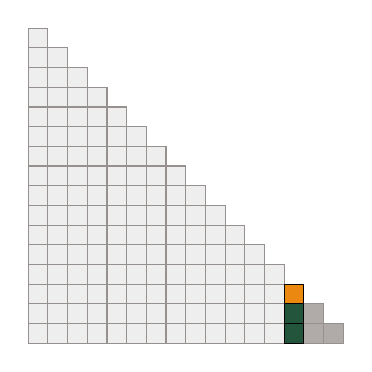
\begin{tikzpicture}[scale=4/16]
  \filldraw[draw=zeroborder, fill=zerocolor] (0, 0) rectangle (1, -1);
  \filldraw[draw=zeroborder, fill=zerocolor] (0, -1) rectangle (1, -2);
  \filldraw[draw=zeroborder, fill=zerocolor] (0, -2) rectangle (1, -3);
  \filldraw[draw=zeroborder, fill=zerocolor] (0, -3) rectangle (1, -4);
  \filldraw[draw=zeroborder, fill=zerocolor] (0, -4) rectangle (1, -5);
  \filldraw[draw=zeroborder, fill=zerocolor] (0, -5) rectangle (1, -6);
  \filldraw[draw=zeroborder, fill=zerocolor] (0, -6) rectangle (1, -7);
  \filldraw[draw=zeroborder, fill=zerocolor] (0, -7) rectangle (1, -8);
  \filldraw[draw=zeroborder, fill=zerocolor] (0, -8) rectangle (1, -9);
  \filldraw[draw=zeroborder, fill=zerocolor] (0, -9) rectangle (1, -10);
  \filldraw[draw=zeroborder, fill=zerocolor] (0, -10) rectangle (1, -11);
  \filldraw[draw=zeroborder, fill=zerocolor] (0, -11) rectangle (1, -12);
  \filldraw[draw=zeroborder, fill=zerocolor] (0, -12) rectangle (1, -13);
  \filldraw[draw=zeroborder, fill=zerocolor] (0, -13) rectangle (1, -14);
  \filldraw[draw=zeroborder, fill=zerocolor] (0, -14) rectangle (1, -15);
  \filldraw[draw=zeroborder, fill=zerocolor] (0, -15) rectangle (1, -16);
  \filldraw[draw=zeroborder, fill=zerocolor] (1, -1) rectangle (2, -2);
  \filldraw[draw=zeroborder, fill=zerocolor] (1, -2) rectangle (2, -3);
  \filldraw[draw=zeroborder, fill=zerocolor] (1, -3) rectangle (2, -4);
  \filldraw[draw=zeroborder, fill=zerocolor] (1, -4) rectangle (2, -5);
  \filldraw[draw=zeroborder, fill=zerocolor] (1, -5) rectangle (2, -6);
  \filldraw[draw=zeroborder, fill=zerocolor] (1, -6) rectangle (2, -7);
  \filldraw[draw=zeroborder, fill=zerocolor] (1, -7) rectangle (2, -8);
  \filldraw[draw=zeroborder, fill=zerocolor] (1, -8) rectangle (2, -9);
  \filldraw[draw=zeroborder, fill=zerocolor] (1, -9) rectangle (2, -10);
  \filldraw[draw=zeroborder, fill=zerocolor] (1, -10) rectangle (2, -11);
  \filldraw[draw=zeroborder, fill=zerocolor] (1, -11) rectangle (2, -12);
  \filldraw[draw=zeroborder, fill=zerocolor] (1, -12) rectangle (2, -13);
  \filldraw[draw=zeroborder, fill=zerocolor] (1, -13) rectangle (2, -14);
  \filldraw[draw=zeroborder, fill=zerocolor] (1, -14) rectangle (2, -15);
  \filldraw[draw=zeroborder, fill=zerocolor] (1, -15) rectangle (2, -16);
  \filldraw[draw=zeroborder, fill=zerocolor] (2, -2) rectangle (3, -3);
  \filldraw[draw=zeroborder, fill=zerocolor] (2, -3) rectangle (3, -4);
  \filldraw[draw=zeroborder, fill=zerocolor] (2, -4) rectangle (3, -5);
  \filldraw[draw=zeroborder, fill=zerocolor] (2, -5) rectangle (3, -6);
  \filldraw[draw=zeroborder, fill=zerocolor] (2, -6) rectangle (3, -7);
  \filldraw[draw=zeroborder, fill=zerocolor] (2, -7) rectangle (3, -8);
  \filldraw[draw=zeroborder, fill=zerocolor] (2, -8) rectangle (3, -9);
  \filldraw[draw=zeroborder, fill=zerocolor] (2, -9) rectangle (3, -10);
  \filldraw[draw=zeroborder, fill=zerocolor] (2, -10) rectangle (3, -11);
  \filldraw[draw=zeroborder, fill=zerocolor] (2, -11) rectangle (3, -12);
  \filldraw[draw=zeroborder, fill=zerocolor] (2, -12) rectangle (3, -13);
  \filldraw[draw=zeroborder, fill=zerocolor] (2, -13) rectangle (3, -14);
  \filldraw[draw=zeroborder, fill=zerocolor] (2, -14) rectangle (3, -15);
  \filldraw[draw=zeroborder, fill=zerocolor] (2, -15) rectangle (3, -16);
  \filldraw[draw=zeroborder, fill=zerocolor] (3, -3) rectangle (4, -4);
  \filldraw[draw=zeroborder, fill=zerocolor] (3, -4) rectangle (4, -5);
  \filldraw[draw=zeroborder, fill=zerocolor] (3, -5) rectangle (4, -6);
  \filldraw[draw=zeroborder, fill=zerocolor] (3, -6) rectangle (4, -7);
  \filldraw[draw=zeroborder, fill=zerocolor] (3, -7) rectangle (4, -8);
  \filldraw[draw=zeroborder, fill=zerocolor] (3, -8) rectangle (4, -9);
  \filldraw[draw=zeroborder, fill=zerocolor] (3, -9) rectangle (4, -10);
  \filldraw[draw=zeroborder, fill=zerocolor] (3, -10) rectangle (4, -11);
  \filldraw[draw=zeroborder, fill=zerocolor] (3, -11) rectangle (4, -12);
  \filldraw[draw=zeroborder, fill=zerocolor] (3, -12) rectangle (4, -13);
  \filldraw[draw=zeroborder, fill=zerocolor] (3, -13) rectangle (4, -14);
  \filldraw[draw=zeroborder, fill=zerocolor] (3, -14) rectangle (4, -15);
  \filldraw[draw=zeroborder, fill=zerocolor] (3, -15) rectangle (4, -16);
  \filldraw[draw=zeroborder, fill=zerocolor] (4, -4) rectangle (5, -5);
  \filldraw[draw=zeroborder, fill=zerocolor] (4, -5) rectangle (5, -6);
  \filldraw[draw=zeroborder, fill=zerocolor] (4, -6) rectangle (5, -7);
  \filldraw[draw=zeroborder, fill=zerocolor] (4, -7) rectangle (5, -8);
  \filldraw[draw=zeroborder, fill=zerocolor] (4, -8) rectangle (5, -9);
  \filldraw[draw=zeroborder, fill=zerocolor] (4, -9) rectangle (5, -10);
  \filldraw[draw=zeroborder, fill=zerocolor] (4, -10) rectangle (5, -11);
  \filldraw[draw=zeroborder, fill=zerocolor] (4, -11) rectangle (5, -12);
  \filldraw[draw=zeroborder, fill=zerocolor] (4, -12) rectangle (5, -13);
  \filldraw[draw=zeroborder, fill=zerocolor] (4, -13) rectangle (5, -14);
  \filldraw[draw=zeroborder, fill=zerocolor] (4, -14) rectangle (5, -15);
  \filldraw[draw=zeroborder, fill=zerocolor] (4, -15) rectangle (5, -16);
  \filldraw[draw=zeroborder, fill=zerocolor] (5, -5) rectangle (6, -6);
  \filldraw[draw=zeroborder, fill=zerocolor] (5, -6) rectangle (6, -7);
  \filldraw[draw=zeroborder, fill=zerocolor] (5, -7) rectangle (6, -8);
  \filldraw[draw=zeroborder, fill=zerocolor] (5, -8) rectangle (6, -9);
  \filldraw[draw=zeroborder, fill=zerocolor] (5, -9) rectangle (6, -10);
  \filldraw[draw=zeroborder, fill=zerocolor] (5, -10) rectangle (6, -11);
  \filldraw[draw=zeroborder, fill=zerocolor] (5, -11) rectangle (6, -12);
  \filldraw[draw=zeroborder, fill=zerocolor] (5, -12) rectangle (6, -13);
  \filldraw[draw=zeroborder, fill=zerocolor] (5, -13) rectangle (6, -14);
  \filldraw[draw=zeroborder, fill=zerocolor] (5, -14) rectangle (6, -15);
  \filldraw[draw=zeroborder, fill=zerocolor] (5, -15) rectangle (6, -16);
  \filldraw[draw=zeroborder, fill=zerocolor] (6, -6) rectangle (7, -7);
  \filldraw[draw=zeroborder, fill=zerocolor] (6, -7) rectangle (7, -8);
  \filldraw[draw=zeroborder, fill=zerocolor] (6, -8) rectangle (7, -9);
  \filldraw[draw=zeroborder, fill=zerocolor] (6, -9) rectangle (7, -10);
  \filldraw[draw=zeroborder, fill=zerocolor] (6, -10) rectangle (7, -11);
  \filldraw[draw=zeroborder, fill=zerocolor] (6, -11) rectangle (7, -12);
  \filldraw[draw=zeroborder, fill=zerocolor] (6, -12) rectangle (7, -13);
  \filldraw[draw=zeroborder, fill=zerocolor] (6, -13) rectangle (7, -14);
  \filldraw[draw=zeroborder, fill=zerocolor] (6, -14) rectangle (7, -15);
  \filldraw[draw=zeroborder, fill=zerocolor] (6, -15) rectangle (7, -16);
  \filldraw[draw=zeroborder, fill=zerocolor] (7, -7) rectangle (8, -8);
  \filldraw[draw=zeroborder, fill=zerocolor] (7, -8) rectangle (8, -9);
  \filldraw[draw=zeroborder, fill=zerocolor] (7, -9) rectangle (8, -10);
  \filldraw[draw=zeroborder, fill=zerocolor] (7, -10) rectangle (8, -11);
  \filldraw[draw=zeroborder, fill=zerocolor] (7, -11) rectangle (8, -12);
  \filldraw[draw=zeroborder, fill=zerocolor] (7, -12) rectangle (8, -13);
  \filldraw[draw=zeroborder, fill=zerocolor] (7, -13) rectangle (8, -14);
  \filldraw[draw=zeroborder, fill=zerocolor] (7, -14) rectangle (8, -15);
  \filldraw[draw=zeroborder, fill=zerocolor] (7, -15) rectangle (8, -16);
  \filldraw[draw=zeroborder, fill=zerocolor] (8, -8) rectangle (9, -9);
  \filldraw[draw=zeroborder, fill=zerocolor] (8, -9) rectangle (9, -10);
  \filldraw[draw=zeroborder, fill=zerocolor] (8, -10) rectangle (9, -11);
  \filldraw[draw=zeroborder, fill=zerocolor] (8, -11) rectangle (9, -12);
  \filldraw[draw=zeroborder, fill=zerocolor] (8, -12) rectangle (9, -13);
  \filldraw[draw=zeroborder, fill=zerocolor] (8, -13) rectangle (9, -14);
  \filldraw[draw=zeroborder, fill=zerocolor] (8, -14) rectangle (9, -15);
  \filldraw[draw=zeroborder, fill=zerocolor] (8, -15) rectangle (9, -16);
  \filldraw[draw=zeroborder, fill=zerocolor] (9, -9) rectangle (10, -10);
  \filldraw[draw=zeroborder, fill=zerocolor] (9, -10) rectangle (10, -11);
  \filldraw[draw=zeroborder, fill=zerocolor] (9, -11) rectangle (10, -12);
  \filldraw[draw=zeroborder, fill=zerocolor] (9, -12) rectangle (10, -13);
  \filldraw[draw=zeroborder, fill=zerocolor] (9, -13) rectangle (10, -14);
  \filldraw[draw=zeroborder, fill=zerocolor] (9, -14) rectangle (10, -15);
  \filldraw[draw=zeroborder, fill=zerocolor] (9, -15) rectangle (10, -16);
  \filldraw[draw=zeroborder, fill=zerocolor] (10, -10) rectangle (11, -11);
  \filldraw[draw=zeroborder, fill=zerocolor] (10, -11) rectangle (11, -12);
  \filldraw[draw=zeroborder, fill=zerocolor] (10, -12) rectangle (11, -13);
  \filldraw[draw=zeroborder, fill=zerocolor] (10, -13) rectangle (11, -14);
  \filldraw[draw=zeroborder, fill=zerocolor] (10, -14) rectangle (11, -15);
  \filldraw[draw=zeroborder, fill=zerocolor] (10, -15) rectangle (11, -16);
  \filldraw[draw=zeroborder, fill=zerocolor] (11, -11) rectangle (12, -12);
  \filldraw[draw=zeroborder, fill=zerocolor] (11, -12) rectangle (12, -13);
  \filldraw[draw=zeroborder, fill=zerocolor] (11, -13) rectangle (12, -14);
  \filldraw[draw=zeroborder, fill=zerocolor] (11, -14) rectangle (12, -15);
  \filldraw[draw=zeroborder, fill=zerocolor] (11, -15) rectangle (12, -16);
  \filldraw[draw=zeroborder, fill=zerocolor] (12, -12) rectangle (13, -13);
  \filldraw[draw=zeroborder, fill=zerocolor] (12, -13) rectangle (13, -14);
  \filldraw[draw=zeroborder, fill=zerocolor] (12, -14) rectangle (13, -15);
  \filldraw[draw=zeroborder, fill=zerocolor] (12, -15) rectangle (13, -16);
  \filldraw[draw=nnzborder, fill=nnzcolor] (14, -14) rectangle (15, -15);
  \filldraw[draw=nnzborder, fill=nnzcolor] (14, -15) rectangle (15, -16);
  \filldraw[draw=nnzborder, fill=nnzcolor] (15, -15) rectangle (16, -16);
  \filldraw[draw=colborder, fill=targetcolor] (13, -13) rectangle (14, -14);
  \filldraw[draw=colborder, fill=selcolor] (13, -14) rectangle (14, -15);
  \filldraw[draw=colborder, fill=selcolor] (13, -15) rectangle (14, -16);
\end{tikzpicture}
%
    \qquad
    \begin{tikzpicture}[baseline]
  \begin{axis}[
    % calculated from Cholesky factor, exactly 16 cm x 16 cm
    width={4cm},
    height={4cm},
    axis lines={none},
    % force axis box to have exactly the right dimensions, ignoring labels
    scale only axis=true,
  ]
  % consistent size bounding box
  \draw [white, line width=0] (-0.1, -0.1) -- (-0.1,  1.1);
  \draw [white, line width=0] ( 1.1, -0.1) -- ( 1.1,  1.1);
  \draw [white, line width=0] (-0.1, -0.1) -- (-1.1, -0.1);
  \draw [white, line width=0] (-0.1,  1.1) -- (-1.1,  1.1);
  \draw [seagreen!15, fill, radius=1.4730958938598633] (0.0014900835088361708, 0.9734602747664127) circle;
  \draw [seagreen, radius=1.4730958938598633] (0.0014900835088361708, 0.9734602747664127) circle;
  \draw [orange!25, fill, radius=0.7365479469299316] (0.0014900835088361708, 0.9734602747664127) circle;
  \draw [orange, radius=0.7365479469299316] (0.0014900835088361708, 0.9734602747664127) circle;
  \addplot [only marks, mark size=1, silver]    table
    {figures/points_knn/all_points.csv};
  \addplot [only marks, mark size=2, lightblue] table
    {figures/points_knn/candidates_03.csv};
  \addplot [only marks, mark size=4, seagreen]  table
    {figures/points_knn/selected_03.csv};
  \addplot [only marks, mark size=4, orange]    table
    {figures/points_knn/target_03.csv};
  \end{axis}
\end{tikzpicture}

  \end{figure}
}
\only<4>{
  \begin{figure}
    \centering
    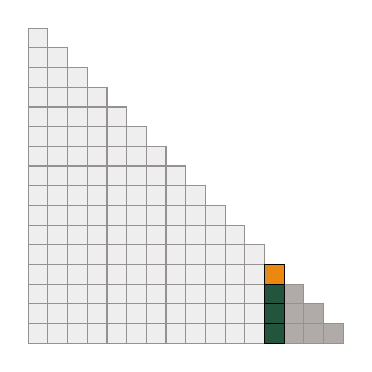
\begin{tikzpicture}[scale=4/16]
  \filldraw[draw=zeroborder, fill=zerocolor] (0, 0) rectangle (1, -1);
  \filldraw[draw=zeroborder, fill=zerocolor] (0, -1) rectangle (1, -2);
  \filldraw[draw=zeroborder, fill=zerocolor] (0, -2) rectangle (1, -3);
  \filldraw[draw=zeroborder, fill=zerocolor] (0, -3) rectangle (1, -4);
  \filldraw[draw=zeroborder, fill=zerocolor] (0, -4) rectangle (1, -5);
  \filldraw[draw=zeroborder, fill=zerocolor] (0, -5) rectangle (1, -6);
  \filldraw[draw=zeroborder, fill=zerocolor] (0, -6) rectangle (1, -7);
  \filldraw[draw=zeroborder, fill=zerocolor] (0, -7) rectangle (1, -8);
  \filldraw[draw=zeroborder, fill=zerocolor] (0, -8) rectangle (1, -9);
  \filldraw[draw=zeroborder, fill=zerocolor] (0, -9) rectangle (1, -10);
  \filldraw[draw=zeroborder, fill=zerocolor] (0, -10) rectangle (1, -11);
  \filldraw[draw=zeroborder, fill=zerocolor] (0, -11) rectangle (1, -12);
  \filldraw[draw=zeroborder, fill=zerocolor] (0, -12) rectangle (1, -13);
  \filldraw[draw=zeroborder, fill=zerocolor] (0, -13) rectangle (1, -14);
  \filldraw[draw=zeroborder, fill=zerocolor] (0, -14) rectangle (1, -15);
  \filldraw[draw=zeroborder, fill=zerocolor] (0, -15) rectangle (1, -16);
  \filldraw[draw=zeroborder, fill=zerocolor] (1, -1) rectangle (2, -2);
  \filldraw[draw=zeroborder, fill=zerocolor] (1, -2) rectangle (2, -3);
  \filldraw[draw=zeroborder, fill=zerocolor] (1, -3) rectangle (2, -4);
  \filldraw[draw=zeroborder, fill=zerocolor] (1, -4) rectangle (2, -5);
  \filldraw[draw=zeroborder, fill=zerocolor] (1, -5) rectangle (2, -6);
  \filldraw[draw=zeroborder, fill=zerocolor] (1, -6) rectangle (2, -7);
  \filldraw[draw=zeroborder, fill=zerocolor] (1, -7) rectangle (2, -8);
  \filldraw[draw=zeroborder, fill=zerocolor] (1, -8) rectangle (2, -9);
  \filldraw[draw=zeroborder, fill=zerocolor] (1, -9) rectangle (2, -10);
  \filldraw[draw=zeroborder, fill=zerocolor] (1, -10) rectangle (2, -11);
  \filldraw[draw=zeroborder, fill=zerocolor] (1, -11) rectangle (2, -12);
  \filldraw[draw=zeroborder, fill=zerocolor] (1, -12) rectangle (2, -13);
  \filldraw[draw=zeroborder, fill=zerocolor] (1, -13) rectangle (2, -14);
  \filldraw[draw=zeroborder, fill=zerocolor] (1, -14) rectangle (2, -15);
  \filldraw[draw=zeroborder, fill=zerocolor] (1, -15) rectangle (2, -16);
  \filldraw[draw=zeroborder, fill=zerocolor] (2, -2) rectangle (3, -3);
  \filldraw[draw=zeroborder, fill=zerocolor] (2, -3) rectangle (3, -4);
  \filldraw[draw=zeroborder, fill=zerocolor] (2, -4) rectangle (3, -5);
  \filldraw[draw=zeroborder, fill=zerocolor] (2, -5) rectangle (3, -6);
  \filldraw[draw=zeroborder, fill=zerocolor] (2, -6) rectangle (3, -7);
  \filldraw[draw=zeroborder, fill=zerocolor] (2, -7) rectangle (3, -8);
  \filldraw[draw=zeroborder, fill=zerocolor] (2, -8) rectangle (3, -9);
  \filldraw[draw=zeroborder, fill=zerocolor] (2, -9) rectangle (3, -10);
  \filldraw[draw=zeroborder, fill=zerocolor] (2, -10) rectangle (3, -11);
  \filldraw[draw=zeroborder, fill=zerocolor] (2, -11) rectangle (3, -12);
  \filldraw[draw=zeroborder, fill=zerocolor] (2, -12) rectangle (3, -13);
  \filldraw[draw=zeroborder, fill=zerocolor] (2, -13) rectangle (3, -14);
  \filldraw[draw=zeroborder, fill=zerocolor] (2, -14) rectangle (3, -15);
  \filldraw[draw=zeroborder, fill=zerocolor] (2, -15) rectangle (3, -16);
  \filldraw[draw=zeroborder, fill=zerocolor] (3, -3) rectangle (4, -4);
  \filldraw[draw=zeroborder, fill=zerocolor] (3, -4) rectangle (4, -5);
  \filldraw[draw=zeroborder, fill=zerocolor] (3, -5) rectangle (4, -6);
  \filldraw[draw=zeroborder, fill=zerocolor] (3, -6) rectangle (4, -7);
  \filldraw[draw=zeroborder, fill=zerocolor] (3, -7) rectangle (4, -8);
  \filldraw[draw=zeroborder, fill=zerocolor] (3, -8) rectangle (4, -9);
  \filldraw[draw=zeroborder, fill=zerocolor] (3, -9) rectangle (4, -10);
  \filldraw[draw=zeroborder, fill=zerocolor] (3, -10) rectangle (4, -11);
  \filldraw[draw=zeroborder, fill=zerocolor] (3, -11) rectangle (4, -12);
  \filldraw[draw=zeroborder, fill=zerocolor] (3, -12) rectangle (4, -13);
  \filldraw[draw=zeroborder, fill=zerocolor] (3, -13) rectangle (4, -14);
  \filldraw[draw=zeroborder, fill=zerocolor] (3, -14) rectangle (4, -15);
  \filldraw[draw=zeroborder, fill=zerocolor] (3, -15) rectangle (4, -16);
  \filldraw[draw=zeroborder, fill=zerocolor] (4, -4) rectangle (5, -5);
  \filldraw[draw=zeroborder, fill=zerocolor] (4, -5) rectangle (5, -6);
  \filldraw[draw=zeroborder, fill=zerocolor] (4, -6) rectangle (5, -7);
  \filldraw[draw=zeroborder, fill=zerocolor] (4, -7) rectangle (5, -8);
  \filldraw[draw=zeroborder, fill=zerocolor] (4, -8) rectangle (5, -9);
  \filldraw[draw=zeroborder, fill=zerocolor] (4, -9) rectangle (5, -10);
  \filldraw[draw=zeroborder, fill=zerocolor] (4, -10) rectangle (5, -11);
  \filldraw[draw=zeroborder, fill=zerocolor] (4, -11) rectangle (5, -12);
  \filldraw[draw=zeroborder, fill=zerocolor] (4, -12) rectangle (5, -13);
  \filldraw[draw=zeroborder, fill=zerocolor] (4, -13) rectangle (5, -14);
  \filldraw[draw=zeroborder, fill=zerocolor] (4, -14) rectangle (5, -15);
  \filldraw[draw=zeroborder, fill=zerocolor] (4, -15) rectangle (5, -16);
  \filldraw[draw=zeroborder, fill=zerocolor] (5, -5) rectangle (6, -6);
  \filldraw[draw=zeroborder, fill=zerocolor] (5, -6) rectangle (6, -7);
  \filldraw[draw=zeroborder, fill=zerocolor] (5, -7) rectangle (6, -8);
  \filldraw[draw=zeroborder, fill=zerocolor] (5, -8) rectangle (6, -9);
  \filldraw[draw=zeroborder, fill=zerocolor] (5, -9) rectangle (6, -10);
  \filldraw[draw=zeroborder, fill=zerocolor] (5, -10) rectangle (6, -11);
  \filldraw[draw=zeroborder, fill=zerocolor] (5, -11) rectangle (6, -12);
  \filldraw[draw=zeroborder, fill=zerocolor] (5, -12) rectangle (6, -13);
  \filldraw[draw=zeroborder, fill=zerocolor] (5, -13) rectangle (6, -14);
  \filldraw[draw=zeroborder, fill=zerocolor] (5, -14) rectangle (6, -15);
  \filldraw[draw=zeroborder, fill=zerocolor] (5, -15) rectangle (6, -16);
  \filldraw[draw=zeroborder, fill=zerocolor] (6, -6) rectangle (7, -7);
  \filldraw[draw=zeroborder, fill=zerocolor] (6, -7) rectangle (7, -8);
  \filldraw[draw=zeroborder, fill=zerocolor] (6, -8) rectangle (7, -9);
  \filldraw[draw=zeroborder, fill=zerocolor] (6, -9) rectangle (7, -10);
  \filldraw[draw=zeroborder, fill=zerocolor] (6, -10) rectangle (7, -11);
  \filldraw[draw=zeroborder, fill=zerocolor] (6, -11) rectangle (7, -12);
  \filldraw[draw=zeroborder, fill=zerocolor] (6, -12) rectangle (7, -13);
  \filldraw[draw=zeroborder, fill=zerocolor] (6, -13) rectangle (7, -14);
  \filldraw[draw=zeroborder, fill=zerocolor] (6, -14) rectangle (7, -15);
  \filldraw[draw=zeroborder, fill=zerocolor] (6, -15) rectangle (7, -16);
  \filldraw[draw=zeroborder, fill=zerocolor] (7, -7) rectangle (8, -8);
  \filldraw[draw=zeroborder, fill=zerocolor] (7, -8) rectangle (8, -9);
  \filldraw[draw=zeroborder, fill=zerocolor] (7, -9) rectangle (8, -10);
  \filldraw[draw=zeroborder, fill=zerocolor] (7, -10) rectangle (8, -11);
  \filldraw[draw=zeroborder, fill=zerocolor] (7, -11) rectangle (8, -12);
  \filldraw[draw=zeroborder, fill=zerocolor] (7, -12) rectangle (8, -13);
  \filldraw[draw=zeroborder, fill=zerocolor] (7, -13) rectangle (8, -14);
  \filldraw[draw=zeroborder, fill=zerocolor] (7, -14) rectangle (8, -15);
  \filldraw[draw=zeroborder, fill=zerocolor] (7, -15) rectangle (8, -16);
  \filldraw[draw=zeroborder, fill=zerocolor] (8, -8) rectangle (9, -9);
  \filldraw[draw=zeroborder, fill=zerocolor] (8, -9) rectangle (9, -10);
  \filldraw[draw=zeroborder, fill=zerocolor] (8, -10) rectangle (9, -11);
  \filldraw[draw=zeroborder, fill=zerocolor] (8, -11) rectangle (9, -12);
  \filldraw[draw=zeroborder, fill=zerocolor] (8, -12) rectangle (9, -13);
  \filldraw[draw=zeroborder, fill=zerocolor] (8, -13) rectangle (9, -14);
  \filldraw[draw=zeroborder, fill=zerocolor] (8, -14) rectangle (9, -15);
  \filldraw[draw=zeroborder, fill=zerocolor] (8, -15) rectangle (9, -16);
  \filldraw[draw=zeroborder, fill=zerocolor] (9, -9) rectangle (10, -10);
  \filldraw[draw=zeroborder, fill=zerocolor] (9, -10) rectangle (10, -11);
  \filldraw[draw=zeroborder, fill=zerocolor] (9, -11) rectangle (10, -12);
  \filldraw[draw=zeroborder, fill=zerocolor] (9, -12) rectangle (10, -13);
  \filldraw[draw=zeroborder, fill=zerocolor] (9, -13) rectangle (10, -14);
  \filldraw[draw=zeroborder, fill=zerocolor] (9, -14) rectangle (10, -15);
  \filldraw[draw=zeroborder, fill=zerocolor] (9, -15) rectangle (10, -16);
  \filldraw[draw=zeroborder, fill=zerocolor] (10, -10) rectangle (11, -11);
  \filldraw[draw=zeroborder, fill=zerocolor] (10, -11) rectangle (11, -12);
  \filldraw[draw=zeroborder, fill=zerocolor] (10, -12) rectangle (11, -13);
  \filldraw[draw=zeroborder, fill=zerocolor] (10, -13) rectangle (11, -14);
  \filldraw[draw=zeroborder, fill=zerocolor] (10, -14) rectangle (11, -15);
  \filldraw[draw=zeroborder, fill=zerocolor] (10, -15) rectangle (11, -16);
  \filldraw[draw=zeroborder, fill=zerocolor] (11, -11) rectangle (12, -12);
  \filldraw[draw=zeroborder, fill=zerocolor] (11, -12) rectangle (12, -13);
  \filldraw[draw=zeroborder, fill=zerocolor] (11, -13) rectangle (12, -14);
  \filldraw[draw=zeroborder, fill=zerocolor] (11, -14) rectangle (12, -15);
  \filldraw[draw=zeroborder, fill=zerocolor] (11, -15) rectangle (12, -16);
  \filldraw[draw=nnzborder, fill=nnzcolor] (13, -13) rectangle (14, -14);
  \filldraw[draw=nnzborder, fill=nnzcolor] (13, -14) rectangle (14, -15);
  \filldraw[draw=nnzborder, fill=nnzcolor] (13, -15) rectangle (14, -16);
  \filldraw[draw=nnzborder, fill=nnzcolor] (14, -14) rectangle (15, -15);
  \filldraw[draw=nnzborder, fill=nnzcolor] (14, -15) rectangle (15, -16);
  \filldraw[draw=nnzborder, fill=nnzcolor] (15, -15) rectangle (16, -16);
  \filldraw[draw=colborder, fill=targetcolor] (12, -12) rectangle (13, -13);
  \filldraw[draw=colborder, fill=selcolor] (12, -13) rectangle (13, -14);
  \filldraw[draw=colborder, fill=selcolor] (12, -14) rectangle (13, -15);
  \filldraw[draw=colborder, fill=selcolor] (12, -15) rectangle (13, -16);
\end{tikzpicture}
%
    \qquad
    \begin{tikzpicture}[baseline]
  \begin{axis}[
    % calculated from Cholesky factor, exactly 16 cm x 16 cm
    width={4cm},
    height={4cm},
    axis lines={none},
    % force axis box to have exactly the right dimensions, ignoring labels
    scale only axis=true,
  ]
  % consistent size bounding box
  \draw [white, line width=0] (-0.1, -0.1) -- (-0.1,  1.1);
  \draw [white, line width=0] ( 1.1, -0.1) -- ( 1.1,  1.1);
  \draw [white, line width=0] (-0.1, -0.1) -- (-1.1, -0.1);
  \draw [white, line width=0] (-0.1,  1.1) -- (-1.1,  1.1);
  \draw [seagreen!15, fill, radius=1.3210153579711914] (0.7345771514092145, 0.11367201992140341) circle;
  \draw [seagreen, radius=1.3210153579711914] (0.7345771514092145, 0.11367201992140341) circle;
  \draw [orange!25, fill, radius=0.6605076789855957] (0.7345771514092145, 0.11367201992140341) circle;
  \draw [orange, radius=0.6605076789855957] (0.7345771514092145, 0.11367201992140341) circle;
  \addplot [only marks, mark size=1, silver]    table
    {figures/points_knn/all_points.csv};
  \addplot [only marks, mark size=2, lightblue] table
    {figures/points_knn/candidates_04.csv};
  \addplot [only marks, mark size=4, seagreen]  table
    {figures/points_knn/selected_04.csv};
  \addplot [only marks, mark size=4, orange]    table
    {figures/points_knn/target_04.csv};
  \end{axis}
\end{tikzpicture}

  \end{figure}
}
\only<5>{
  \begin{figure}
    \centering
    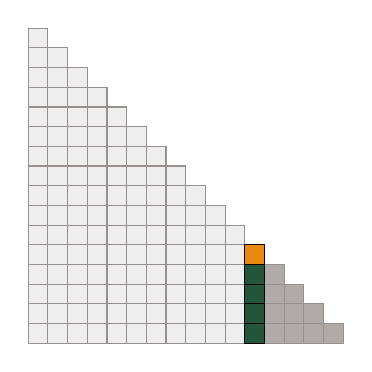
\begin{tikzpicture}[scale=4/16]
  \filldraw[draw=zeroborder, fill=zerocolor] (0, 0) rectangle (1, -1);
  \filldraw[draw=zeroborder, fill=zerocolor] (0, -1) rectangle (1, -2);
  \filldraw[draw=zeroborder, fill=zerocolor] (0, -2) rectangle (1, -3);
  \filldraw[draw=zeroborder, fill=zerocolor] (0, -3) rectangle (1, -4);
  \filldraw[draw=zeroborder, fill=zerocolor] (0, -4) rectangle (1, -5);
  \filldraw[draw=zeroborder, fill=zerocolor] (0, -5) rectangle (1, -6);
  \filldraw[draw=zeroborder, fill=zerocolor] (0, -6) rectangle (1, -7);
  \filldraw[draw=zeroborder, fill=zerocolor] (0, -7) rectangle (1, -8);
  \filldraw[draw=zeroborder, fill=zerocolor] (0, -8) rectangle (1, -9);
  \filldraw[draw=zeroborder, fill=zerocolor] (0, -9) rectangle (1, -10);
  \filldraw[draw=zeroborder, fill=zerocolor] (0, -10) rectangle (1, -11);
  \filldraw[draw=zeroborder, fill=zerocolor] (0, -11) rectangle (1, -12);
  \filldraw[draw=zeroborder, fill=zerocolor] (0, -12) rectangle (1, -13);
  \filldraw[draw=zeroborder, fill=zerocolor] (0, -13) rectangle (1, -14);
  \filldraw[draw=zeroborder, fill=zerocolor] (0, -14) rectangle (1, -15);
  \filldraw[draw=zeroborder, fill=zerocolor] (0, -15) rectangle (1, -16);
  \filldraw[draw=zeroborder, fill=zerocolor] (1, -1) rectangle (2, -2);
  \filldraw[draw=zeroborder, fill=zerocolor] (1, -2) rectangle (2, -3);
  \filldraw[draw=zeroborder, fill=zerocolor] (1, -3) rectangle (2, -4);
  \filldraw[draw=zeroborder, fill=zerocolor] (1, -4) rectangle (2, -5);
  \filldraw[draw=zeroborder, fill=zerocolor] (1, -5) rectangle (2, -6);
  \filldraw[draw=zeroborder, fill=zerocolor] (1, -6) rectangle (2, -7);
  \filldraw[draw=zeroborder, fill=zerocolor] (1, -7) rectangle (2, -8);
  \filldraw[draw=zeroborder, fill=zerocolor] (1, -8) rectangle (2, -9);
  \filldraw[draw=zeroborder, fill=zerocolor] (1, -9) rectangle (2, -10);
  \filldraw[draw=zeroborder, fill=zerocolor] (1, -10) rectangle (2, -11);
  \filldraw[draw=zeroborder, fill=zerocolor] (1, -11) rectangle (2, -12);
  \filldraw[draw=zeroborder, fill=zerocolor] (1, -12) rectangle (2, -13);
  \filldraw[draw=zeroborder, fill=zerocolor] (1, -13) rectangle (2, -14);
  \filldraw[draw=zeroborder, fill=zerocolor] (1, -14) rectangle (2, -15);
  \filldraw[draw=zeroborder, fill=zerocolor] (1, -15) rectangle (2, -16);
  \filldraw[draw=zeroborder, fill=zerocolor] (2, -2) rectangle (3, -3);
  \filldraw[draw=zeroborder, fill=zerocolor] (2, -3) rectangle (3, -4);
  \filldraw[draw=zeroborder, fill=zerocolor] (2, -4) rectangle (3, -5);
  \filldraw[draw=zeroborder, fill=zerocolor] (2, -5) rectangle (3, -6);
  \filldraw[draw=zeroborder, fill=zerocolor] (2, -6) rectangle (3, -7);
  \filldraw[draw=zeroborder, fill=zerocolor] (2, -7) rectangle (3, -8);
  \filldraw[draw=zeroborder, fill=zerocolor] (2, -8) rectangle (3, -9);
  \filldraw[draw=zeroborder, fill=zerocolor] (2, -9) rectangle (3, -10);
  \filldraw[draw=zeroborder, fill=zerocolor] (2, -10) rectangle (3, -11);
  \filldraw[draw=zeroborder, fill=zerocolor] (2, -11) rectangle (3, -12);
  \filldraw[draw=zeroborder, fill=zerocolor] (2, -12) rectangle (3, -13);
  \filldraw[draw=zeroborder, fill=zerocolor] (2, -13) rectangle (3, -14);
  \filldraw[draw=zeroborder, fill=zerocolor] (2, -14) rectangle (3, -15);
  \filldraw[draw=zeroborder, fill=zerocolor] (2, -15) rectangle (3, -16);
  \filldraw[draw=zeroborder, fill=zerocolor] (3, -3) rectangle (4, -4);
  \filldraw[draw=zeroborder, fill=zerocolor] (3, -4) rectangle (4, -5);
  \filldraw[draw=zeroborder, fill=zerocolor] (3, -5) rectangle (4, -6);
  \filldraw[draw=zeroborder, fill=zerocolor] (3, -6) rectangle (4, -7);
  \filldraw[draw=zeroborder, fill=zerocolor] (3, -7) rectangle (4, -8);
  \filldraw[draw=zeroborder, fill=zerocolor] (3, -8) rectangle (4, -9);
  \filldraw[draw=zeroborder, fill=zerocolor] (3, -9) rectangle (4, -10);
  \filldraw[draw=zeroborder, fill=zerocolor] (3, -10) rectangle (4, -11);
  \filldraw[draw=zeroborder, fill=zerocolor] (3, -11) rectangle (4, -12);
  \filldraw[draw=zeroborder, fill=zerocolor] (3, -12) rectangle (4, -13);
  \filldraw[draw=zeroborder, fill=zerocolor] (3, -13) rectangle (4, -14);
  \filldraw[draw=zeroborder, fill=zerocolor] (3, -14) rectangle (4, -15);
  \filldraw[draw=zeroborder, fill=zerocolor] (3, -15) rectangle (4, -16);
  \filldraw[draw=zeroborder, fill=zerocolor] (4, -4) rectangle (5, -5);
  \filldraw[draw=zeroborder, fill=zerocolor] (4, -5) rectangle (5, -6);
  \filldraw[draw=zeroborder, fill=zerocolor] (4, -6) rectangle (5, -7);
  \filldraw[draw=zeroborder, fill=zerocolor] (4, -7) rectangle (5, -8);
  \filldraw[draw=zeroborder, fill=zerocolor] (4, -8) rectangle (5, -9);
  \filldraw[draw=zeroborder, fill=zerocolor] (4, -9) rectangle (5, -10);
  \filldraw[draw=zeroborder, fill=zerocolor] (4, -10) rectangle (5, -11);
  \filldraw[draw=zeroborder, fill=zerocolor] (4, -11) rectangle (5, -12);
  \filldraw[draw=zeroborder, fill=zerocolor] (4, -12) rectangle (5, -13);
  \filldraw[draw=zeroborder, fill=zerocolor] (4, -13) rectangle (5, -14);
  \filldraw[draw=zeroborder, fill=zerocolor] (4, -14) rectangle (5, -15);
  \filldraw[draw=zeroborder, fill=zerocolor] (4, -15) rectangle (5, -16);
  \filldraw[draw=zeroborder, fill=zerocolor] (5, -5) rectangle (6, -6);
  \filldraw[draw=zeroborder, fill=zerocolor] (5, -6) rectangle (6, -7);
  \filldraw[draw=zeroborder, fill=zerocolor] (5, -7) rectangle (6, -8);
  \filldraw[draw=zeroborder, fill=zerocolor] (5, -8) rectangle (6, -9);
  \filldraw[draw=zeroborder, fill=zerocolor] (5, -9) rectangle (6, -10);
  \filldraw[draw=zeroborder, fill=zerocolor] (5, -10) rectangle (6, -11);
  \filldraw[draw=zeroborder, fill=zerocolor] (5, -11) rectangle (6, -12);
  \filldraw[draw=zeroborder, fill=zerocolor] (5, -12) rectangle (6, -13);
  \filldraw[draw=zeroborder, fill=zerocolor] (5, -13) rectangle (6, -14);
  \filldraw[draw=zeroborder, fill=zerocolor] (5, -14) rectangle (6, -15);
  \filldraw[draw=zeroborder, fill=zerocolor] (5, -15) rectangle (6, -16);
  \filldraw[draw=zeroborder, fill=zerocolor] (6, -6) rectangle (7, -7);
  \filldraw[draw=zeroborder, fill=zerocolor] (6, -7) rectangle (7, -8);
  \filldraw[draw=zeroborder, fill=zerocolor] (6, -8) rectangle (7, -9);
  \filldraw[draw=zeroborder, fill=zerocolor] (6, -9) rectangle (7, -10);
  \filldraw[draw=zeroborder, fill=zerocolor] (6, -10) rectangle (7, -11);
  \filldraw[draw=zeroborder, fill=zerocolor] (6, -11) rectangle (7, -12);
  \filldraw[draw=zeroborder, fill=zerocolor] (6, -12) rectangle (7, -13);
  \filldraw[draw=zeroborder, fill=zerocolor] (6, -13) rectangle (7, -14);
  \filldraw[draw=zeroborder, fill=zerocolor] (6, -14) rectangle (7, -15);
  \filldraw[draw=zeroborder, fill=zerocolor] (6, -15) rectangle (7, -16);
  \filldraw[draw=zeroborder, fill=zerocolor] (7, -7) rectangle (8, -8);
  \filldraw[draw=zeroborder, fill=zerocolor] (7, -8) rectangle (8, -9);
  \filldraw[draw=zeroborder, fill=zerocolor] (7, -9) rectangle (8, -10);
  \filldraw[draw=zeroborder, fill=zerocolor] (7, -10) rectangle (8, -11);
  \filldraw[draw=zeroborder, fill=zerocolor] (7, -11) rectangle (8, -12);
  \filldraw[draw=zeroborder, fill=zerocolor] (7, -12) rectangle (8, -13);
  \filldraw[draw=zeroborder, fill=zerocolor] (7, -13) rectangle (8, -14);
  \filldraw[draw=zeroborder, fill=zerocolor] (7, -14) rectangle (8, -15);
  \filldraw[draw=zeroborder, fill=zerocolor] (7, -15) rectangle (8, -16);
  \filldraw[draw=zeroborder, fill=zerocolor] (8, -8) rectangle (9, -9);
  \filldraw[draw=zeroborder, fill=zerocolor] (8, -9) rectangle (9, -10);
  \filldraw[draw=zeroborder, fill=zerocolor] (8, -10) rectangle (9, -11);
  \filldraw[draw=zeroborder, fill=zerocolor] (8, -11) rectangle (9, -12);
  \filldraw[draw=zeroborder, fill=zerocolor] (8, -12) rectangle (9, -13);
  \filldraw[draw=zeroborder, fill=zerocolor] (8, -13) rectangle (9, -14);
  \filldraw[draw=zeroborder, fill=zerocolor] (8, -14) rectangle (9, -15);
  \filldraw[draw=zeroborder, fill=zerocolor] (8, -15) rectangle (9, -16);
  \filldraw[draw=zeroborder, fill=zerocolor] (9, -9) rectangle (10, -10);
  \filldraw[draw=zeroborder, fill=zerocolor] (9, -10) rectangle (10, -11);
  \filldraw[draw=zeroborder, fill=zerocolor] (9, -11) rectangle (10, -12);
  \filldraw[draw=zeroborder, fill=zerocolor] (9, -12) rectangle (10, -13);
  \filldraw[draw=zeroborder, fill=zerocolor] (9, -13) rectangle (10, -14);
  \filldraw[draw=zeroborder, fill=zerocolor] (9, -14) rectangle (10, -15);
  \filldraw[draw=zeroborder, fill=zerocolor] (9, -15) rectangle (10, -16);
  \filldraw[draw=zeroborder, fill=zerocolor] (10, -10) rectangle (11, -11);
  \filldraw[draw=zeroborder, fill=zerocolor] (10, -11) rectangle (11, -12);
  \filldraw[draw=zeroborder, fill=zerocolor] (10, -12) rectangle (11, -13);
  \filldraw[draw=zeroborder, fill=zerocolor] (10, -13) rectangle (11, -14);
  \filldraw[draw=zeroborder, fill=zerocolor] (10, -14) rectangle (11, -15);
  \filldraw[draw=zeroborder, fill=zerocolor] (10, -15) rectangle (11, -16);
  \filldraw[draw=nnzborder, fill=nnzcolor] (12, -12) rectangle (13, -13);
  \filldraw[draw=nnzborder, fill=nnzcolor] (12, -13) rectangle (13, -14);
  \filldraw[draw=nnzborder, fill=nnzcolor] (12, -14) rectangle (13, -15);
  \filldraw[draw=nnzborder, fill=nnzcolor] (12, -15) rectangle (13, -16);
  \filldraw[draw=nnzborder, fill=nnzcolor] (13, -13) rectangle (14, -14);
  \filldraw[draw=nnzborder, fill=nnzcolor] (13, -14) rectangle (14, -15);
  \filldraw[draw=nnzborder, fill=nnzcolor] (13, -15) rectangle (14, -16);
  \filldraw[draw=nnzborder, fill=nnzcolor] (14, -14) rectangle (15, -15);
  \filldraw[draw=nnzborder, fill=nnzcolor] (14, -15) rectangle (15, -16);
  \filldraw[draw=nnzborder, fill=nnzcolor] (15, -15) rectangle (16, -16);
  \filldraw[draw=colborder, fill=targetcolor] (11, -11) rectangle (12, -12);
  \filldraw[draw=colborder, fill=selcolor] (11, -12) rectangle (12, -13);
  \filldraw[draw=colborder, fill=selcolor] (11, -13) rectangle (12, -14);
  \filldraw[draw=colborder, fill=selcolor] (11, -14) rectangle (12, -15);
  \filldraw[draw=colborder, fill=selcolor] (11, -15) rectangle (12, -16);
\end{tikzpicture}
%
    \qquad
    \begin{tikzpicture}[baseline]
  \begin{axis}[
    % calculated from Cholesky factor, exactly 16 cm x 16 cm
    width={4cm},
    height={4cm},
    axis lines={none},
    % force axis box to have exactly the right dimensions, ignoring labels
    scale only axis=true,
  ]
  % consistent size bounding box
  \draw [white, line width=0] (-0.1, -0.1) -- (-0.1,  1.1);
  \draw [white, line width=0] ( 1.1, -0.1) -- ( 1.1,  1.1);
  \draw [white, line width=0] (-0.1, -0.1) -- (-1.1, -0.1);
  \draw [white, line width=0] (-0.1,  1.1) -- (-1.1,  1.1);
  \addplot [only marks, mark size=1, silver]    table
    {figures/points_cknn/all_points.csv};
  \addplot [only marks, mark size=2, lightblue] table
    {figures/points_cknn/candidates.csv};
  \addplot [only marks, mark size=4, seagreen]  table
    {figures/points_cknn/selected_05.csv};
  \addplot [only marks, mark size=4, orange]    table
    {figures/points_cknn/target.csv};
  \end{axis}
\end{tikzpicture}

  \end{figure}
}
\only<6>{
  \begin{figure}
    \centering
    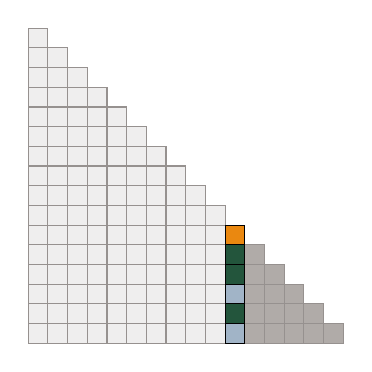
\begin{tikzpicture}[scale=4/16]
  \filldraw[draw=zeroborder, fill=zerocolor] (0, 0) rectangle (1, -1);
  \filldraw[draw=zeroborder, fill=zerocolor] (0, -1) rectangle (1, -2);
  \filldraw[draw=zeroborder, fill=zerocolor] (0, -2) rectangle (1, -3);
  \filldraw[draw=zeroborder, fill=zerocolor] (0, -3) rectangle (1, -4);
  \filldraw[draw=zeroborder, fill=zerocolor] (0, -4) rectangle (1, -5);
  \filldraw[draw=zeroborder, fill=zerocolor] (0, -5) rectangle (1, -6);
  \filldraw[draw=zeroborder, fill=zerocolor] (0, -6) rectangle (1, -7);
  \filldraw[draw=zeroborder, fill=zerocolor] (0, -7) rectangle (1, -8);
  \filldraw[draw=zeroborder, fill=zerocolor] (0, -8) rectangle (1, -9);
  \filldraw[draw=zeroborder, fill=zerocolor] (0, -9) rectangle (1, -10);
  \filldraw[draw=zeroborder, fill=zerocolor] (0, -10) rectangle (1, -11);
  \filldraw[draw=zeroborder, fill=zerocolor] (0, -11) rectangle (1, -12);
  \filldraw[draw=zeroborder, fill=zerocolor] (0, -12) rectangle (1, -13);
  \filldraw[draw=zeroborder, fill=zerocolor] (0, -13) rectangle (1, -14);
  \filldraw[draw=zeroborder, fill=zerocolor] (0, -14) rectangle (1, -15);
  \filldraw[draw=zeroborder, fill=zerocolor] (0, -15) rectangle (1, -16);
  \filldraw[draw=zeroborder, fill=zerocolor] (1, -1) rectangle (2, -2);
  \filldraw[draw=zeroborder, fill=zerocolor] (1, -2) rectangle (2, -3);
  \filldraw[draw=zeroborder, fill=zerocolor] (1, -3) rectangle (2, -4);
  \filldraw[draw=zeroborder, fill=zerocolor] (1, -4) rectangle (2, -5);
  \filldraw[draw=zeroborder, fill=zerocolor] (1, -5) rectangle (2, -6);
  \filldraw[draw=zeroborder, fill=zerocolor] (1, -6) rectangle (2, -7);
  \filldraw[draw=zeroborder, fill=zerocolor] (1, -7) rectangle (2, -8);
  \filldraw[draw=zeroborder, fill=zerocolor] (1, -8) rectangle (2, -9);
  \filldraw[draw=zeroborder, fill=zerocolor] (1, -9) rectangle (2, -10);
  \filldraw[draw=zeroborder, fill=zerocolor] (1, -10) rectangle (2, -11);
  \filldraw[draw=zeroborder, fill=zerocolor] (1, -11) rectangle (2, -12);
  \filldraw[draw=zeroborder, fill=zerocolor] (1, -12) rectangle (2, -13);
  \filldraw[draw=zeroborder, fill=zerocolor] (1, -13) rectangle (2, -14);
  \filldraw[draw=zeroborder, fill=zerocolor] (1, -14) rectangle (2, -15);
  \filldraw[draw=zeroborder, fill=zerocolor] (1, -15) rectangle (2, -16);
  \filldraw[draw=zeroborder, fill=zerocolor] (2, -2) rectangle (3, -3);
  \filldraw[draw=zeroborder, fill=zerocolor] (2, -3) rectangle (3, -4);
  \filldraw[draw=zeroborder, fill=zerocolor] (2, -4) rectangle (3, -5);
  \filldraw[draw=zeroborder, fill=zerocolor] (2, -5) rectangle (3, -6);
  \filldraw[draw=zeroborder, fill=zerocolor] (2, -6) rectangle (3, -7);
  \filldraw[draw=zeroborder, fill=zerocolor] (2, -7) rectangle (3, -8);
  \filldraw[draw=zeroborder, fill=zerocolor] (2, -8) rectangle (3, -9);
  \filldraw[draw=zeroborder, fill=zerocolor] (2, -9) rectangle (3, -10);
  \filldraw[draw=zeroborder, fill=zerocolor] (2, -10) rectangle (3, -11);
  \filldraw[draw=zeroborder, fill=zerocolor] (2, -11) rectangle (3, -12);
  \filldraw[draw=zeroborder, fill=zerocolor] (2, -12) rectangle (3, -13);
  \filldraw[draw=zeroborder, fill=zerocolor] (2, -13) rectangle (3, -14);
  \filldraw[draw=zeroborder, fill=zerocolor] (2, -14) rectangle (3, -15);
  \filldraw[draw=zeroborder, fill=zerocolor] (2, -15) rectangle (3, -16);
  \filldraw[draw=zeroborder, fill=zerocolor] (3, -3) rectangle (4, -4);
  \filldraw[draw=zeroborder, fill=zerocolor] (3, -4) rectangle (4, -5);
  \filldraw[draw=zeroborder, fill=zerocolor] (3, -5) rectangle (4, -6);
  \filldraw[draw=zeroborder, fill=zerocolor] (3, -6) rectangle (4, -7);
  \filldraw[draw=zeroborder, fill=zerocolor] (3, -7) rectangle (4, -8);
  \filldraw[draw=zeroborder, fill=zerocolor] (3, -8) rectangle (4, -9);
  \filldraw[draw=zeroborder, fill=zerocolor] (3, -9) rectangle (4, -10);
  \filldraw[draw=zeroborder, fill=zerocolor] (3, -10) rectangle (4, -11);
  \filldraw[draw=zeroborder, fill=zerocolor] (3, -11) rectangle (4, -12);
  \filldraw[draw=zeroborder, fill=zerocolor] (3, -12) rectangle (4, -13);
  \filldraw[draw=zeroborder, fill=zerocolor] (3, -13) rectangle (4, -14);
  \filldraw[draw=zeroborder, fill=zerocolor] (3, -14) rectangle (4, -15);
  \filldraw[draw=zeroborder, fill=zerocolor] (3, -15) rectangle (4, -16);
  \filldraw[draw=zeroborder, fill=zerocolor] (4, -4) rectangle (5, -5);
  \filldraw[draw=zeroborder, fill=zerocolor] (4, -5) rectangle (5, -6);
  \filldraw[draw=zeroborder, fill=zerocolor] (4, -6) rectangle (5, -7);
  \filldraw[draw=zeroborder, fill=zerocolor] (4, -7) rectangle (5, -8);
  \filldraw[draw=zeroborder, fill=zerocolor] (4, -8) rectangle (5, -9);
  \filldraw[draw=zeroborder, fill=zerocolor] (4, -9) rectangle (5, -10);
  \filldraw[draw=zeroborder, fill=zerocolor] (4, -10) rectangle (5, -11);
  \filldraw[draw=zeroborder, fill=zerocolor] (4, -11) rectangle (5, -12);
  \filldraw[draw=zeroborder, fill=zerocolor] (4, -12) rectangle (5, -13);
  \filldraw[draw=zeroborder, fill=zerocolor] (4, -13) rectangle (5, -14);
  \filldraw[draw=zeroborder, fill=zerocolor] (4, -14) rectangle (5, -15);
  \filldraw[draw=zeroborder, fill=zerocolor] (4, -15) rectangle (5, -16);
  \filldraw[draw=zeroborder, fill=zerocolor] (5, -5) rectangle (6, -6);
  \filldraw[draw=zeroborder, fill=zerocolor] (5, -6) rectangle (6, -7);
  \filldraw[draw=zeroborder, fill=zerocolor] (5, -7) rectangle (6, -8);
  \filldraw[draw=zeroborder, fill=zerocolor] (5, -8) rectangle (6, -9);
  \filldraw[draw=zeroborder, fill=zerocolor] (5, -9) rectangle (6, -10);
  \filldraw[draw=zeroborder, fill=zerocolor] (5, -10) rectangle (6, -11);
  \filldraw[draw=zeroborder, fill=zerocolor] (5, -11) rectangle (6, -12);
  \filldraw[draw=zeroborder, fill=zerocolor] (5, -12) rectangle (6, -13);
  \filldraw[draw=zeroborder, fill=zerocolor] (5, -13) rectangle (6, -14);
  \filldraw[draw=zeroborder, fill=zerocolor] (5, -14) rectangle (6, -15);
  \filldraw[draw=zeroborder, fill=zerocolor] (5, -15) rectangle (6, -16);
  \filldraw[draw=zeroborder, fill=zerocolor] (6, -6) rectangle (7, -7);
  \filldraw[draw=zeroborder, fill=zerocolor] (6, -7) rectangle (7, -8);
  \filldraw[draw=zeroborder, fill=zerocolor] (6, -8) rectangle (7, -9);
  \filldraw[draw=zeroborder, fill=zerocolor] (6, -9) rectangle (7, -10);
  \filldraw[draw=zeroborder, fill=zerocolor] (6, -10) rectangle (7, -11);
  \filldraw[draw=zeroborder, fill=zerocolor] (6, -11) rectangle (7, -12);
  \filldraw[draw=zeroborder, fill=zerocolor] (6, -12) rectangle (7, -13);
  \filldraw[draw=zeroborder, fill=zerocolor] (6, -13) rectangle (7, -14);
  \filldraw[draw=zeroborder, fill=zerocolor] (6, -14) rectangle (7, -15);
  \filldraw[draw=zeroborder, fill=zerocolor] (6, -15) rectangle (7, -16);
  \filldraw[draw=zeroborder, fill=zerocolor] (7, -7) rectangle (8, -8);
  \filldraw[draw=zeroborder, fill=zerocolor] (7, -8) rectangle (8, -9);
  \filldraw[draw=zeroborder, fill=zerocolor] (7, -9) rectangle (8, -10);
  \filldraw[draw=zeroborder, fill=zerocolor] (7, -10) rectangle (8, -11);
  \filldraw[draw=zeroborder, fill=zerocolor] (7, -11) rectangle (8, -12);
  \filldraw[draw=zeroborder, fill=zerocolor] (7, -12) rectangle (8, -13);
  \filldraw[draw=zeroborder, fill=zerocolor] (7, -13) rectangle (8, -14);
  \filldraw[draw=zeroborder, fill=zerocolor] (7, -14) rectangle (8, -15);
  \filldraw[draw=zeroborder, fill=zerocolor] (7, -15) rectangle (8, -16);
  \filldraw[draw=zeroborder, fill=zerocolor] (8, -8) rectangle (9, -9);
  \filldraw[draw=zeroborder, fill=zerocolor] (8, -9) rectangle (9, -10);
  \filldraw[draw=zeroborder, fill=zerocolor] (8, -10) rectangle (9, -11);
  \filldraw[draw=zeroborder, fill=zerocolor] (8, -11) rectangle (9, -12);
  \filldraw[draw=zeroborder, fill=zerocolor] (8, -12) rectangle (9, -13);
  \filldraw[draw=zeroborder, fill=zerocolor] (8, -13) rectangle (9, -14);
  \filldraw[draw=zeroborder, fill=zerocolor] (8, -14) rectangle (9, -15);
  \filldraw[draw=zeroborder, fill=zerocolor] (8, -15) rectangle (9, -16);
  \filldraw[draw=zeroborder, fill=zerocolor] (9, -9) rectangle (10, -10);
  \filldraw[draw=zeroborder, fill=zerocolor] (9, -10) rectangle (10, -11);
  \filldraw[draw=zeroborder, fill=zerocolor] (9, -11) rectangle (10, -12);
  \filldraw[draw=zeroborder, fill=zerocolor] (9, -12) rectangle (10, -13);
  \filldraw[draw=zeroborder, fill=zerocolor] (9, -13) rectangle (10, -14);
  \filldraw[draw=zeroborder, fill=zerocolor] (9, -14) rectangle (10, -15);
  \filldraw[draw=zeroborder, fill=zerocolor] (9, -15) rectangle (10, -16);
  \filldraw[draw=nnzborder, fill=nnzcolor] (11, -11) rectangle (12, -12);
  \filldraw[draw=nnzborder, fill=nnzcolor] (11, -12) rectangle (12, -13);
  \filldraw[draw=nnzborder, fill=nnzcolor] (11, -13) rectangle (12, -14);
  \filldraw[draw=nnzborder, fill=nnzcolor] (11, -14) rectangle (12, -15);
  \filldraw[draw=nnzborder, fill=nnzcolor] (11, -15) rectangle (12, -16);
  \filldraw[draw=nnzborder, fill=nnzcolor] (12, -12) rectangle (13, -13);
  \filldraw[draw=nnzborder, fill=nnzcolor] (12, -13) rectangle (13, -14);
  \filldraw[draw=nnzborder, fill=nnzcolor] (12, -14) rectangle (13, -15);
  \filldraw[draw=nnzborder, fill=nnzcolor] (12, -15) rectangle (13, -16);
  \filldraw[draw=nnzborder, fill=nnzcolor] (13, -13) rectangle (14, -14);
  \filldraw[draw=nnzborder, fill=nnzcolor] (13, -14) rectangle (14, -15);
  \filldraw[draw=nnzborder, fill=nnzcolor] (13, -15) rectangle (14, -16);
  \filldraw[draw=nnzborder, fill=nnzcolor] (14, -14) rectangle (15, -15);
  \filldraw[draw=nnzborder, fill=nnzcolor] (14, -15) rectangle (15, -16);
  \filldraw[draw=nnzborder, fill=nnzcolor] (15, -15) rectangle (16, -16);
  \filldraw[draw=colborder, fill=targetcolor] (10, -10) rectangle (11, -11);
  \filldraw[draw=colborder, fill=selcolor] (10, -11) rectangle (11, -12);
  \filldraw[draw=colborder, fill=selcolor] (10, -12) rectangle (11, -13);
  \filldraw[draw=colborder, fill=candcolor] (10, -13) rectangle (11, -14);
  \filldraw[draw=colborder, fill=selcolor] (10, -14) rectangle (11, -15);
  \filldraw[draw=colborder, fill=candcolor] (10, -15) rectangle (11, -16);
\end{tikzpicture}
%
    \qquad
    \begin{tikzpicture}[baseline]
  \begin{axis}[
    % calculated from Cholesky factor, exactly 16 cm x 16 cm
    width={4cm},
    height={4cm},
    axis lines={none},
    % force axis box to have exactly the right dimensions, ignoring labels
    scale only axis=true,
  ]
  % consistent size bounding box
  \draw [white, line width=0] (-0.1, -0.1) -- (-0.1,  1.1);
  \draw [white, line width=0] ( 1.1, -0.1) -- ( 1.1,  1.1);
  \draw [white, line width=0] (-0.1, -0.1) -- (-1.1, -0.1);
  \draw [white, line width=0] (-0.1,  1.1) -- (-1.1,  1.1);
  \draw [seagreen!15, fill, radius=0.8034806251525879] (0.8917110704451572, 0.5851629398909081) circle;
  \draw [seagreen, radius=0.8034806251525879] (0.8917110704451572, 0.5851629398909081) circle;
  \draw [orange!25, fill, radius=0.40174031257629395] (0.8917110704451572, 0.5851629398909081) circle;
  \draw [orange, radius=0.40174031257629395] (0.8917110704451572, 0.5851629398909081) circle;
  \addplot [only marks, mark size=1, silver]    table
    {figures/points_knn/all_points.csv};
  \addplot [only marks, mark size=2, lightblue] table
    {figures/points_knn/candidates_06.csv};
  \addplot [only marks, mark size=4, seagreen]  table
    {figures/points_knn/selected_06.csv};
  \addplot [only marks, mark size=4, orange]    table
    {figures/points_knn/target_06.csv};
  \end{axis}
\end{tikzpicture}

  \end{figure}
}
\only<7>{
  \begin{figure}
    \centering
    \begin{tikzpicture}[scale=4/16]
  \filldraw[draw=zeroborder, fill=zerocolor] (0, 0) rectangle (1, -1);
  \filldraw[draw=zeroborder, fill=zerocolor] (0, -1) rectangle (1, -2);
  \filldraw[draw=zeroborder, fill=zerocolor] (0, -2) rectangle (1, -3);
  \filldraw[draw=zeroborder, fill=zerocolor] (0, -3) rectangle (1, -4);
  \filldraw[draw=zeroborder, fill=zerocolor] (0, -4) rectangle (1, -5);
  \filldraw[draw=zeroborder, fill=zerocolor] (0, -5) rectangle (1, -6);
  \filldraw[draw=zeroborder, fill=zerocolor] (0, -6) rectangle (1, -7);
  \filldraw[draw=zeroborder, fill=zerocolor] (0, -7) rectangle (1, -8);
  \filldraw[draw=zeroborder, fill=zerocolor] (0, -8) rectangle (1, -9);
  \filldraw[draw=zeroborder, fill=zerocolor] (0, -9) rectangle (1, -10);
  \filldraw[draw=zeroborder, fill=zerocolor] (0, -10) rectangle (1, -11);
  \filldraw[draw=zeroborder, fill=zerocolor] (0, -11) rectangle (1, -12);
  \filldraw[draw=zeroborder, fill=zerocolor] (0, -12) rectangle (1, -13);
  \filldraw[draw=zeroborder, fill=zerocolor] (0, -13) rectangle (1, -14);
  \filldraw[draw=zeroborder, fill=zerocolor] (0, -14) rectangle (1, -15);
  \filldraw[draw=zeroborder, fill=zerocolor] (0, -15) rectangle (1, -16);
  \filldraw[draw=zeroborder, fill=zerocolor] (1, -1) rectangle (2, -2);
  \filldraw[draw=zeroborder, fill=zerocolor] (1, -2) rectangle (2, -3);
  \filldraw[draw=zeroborder, fill=zerocolor] (1, -3) rectangle (2, -4);
  \filldraw[draw=zeroborder, fill=zerocolor] (1, -4) rectangle (2, -5);
  \filldraw[draw=zeroborder, fill=zerocolor] (1, -5) rectangle (2, -6);
  \filldraw[draw=zeroborder, fill=zerocolor] (1, -6) rectangle (2, -7);
  \filldraw[draw=zeroborder, fill=zerocolor] (1, -7) rectangle (2, -8);
  \filldraw[draw=zeroborder, fill=zerocolor] (1, -8) rectangle (2, -9);
  \filldraw[draw=zeroborder, fill=zerocolor] (1, -9) rectangle (2, -10);
  \filldraw[draw=zeroborder, fill=zerocolor] (1, -10) rectangle (2, -11);
  \filldraw[draw=zeroborder, fill=zerocolor] (1, -11) rectangle (2, -12);
  \filldraw[draw=zeroborder, fill=zerocolor] (1, -12) rectangle (2, -13);
  \filldraw[draw=zeroborder, fill=zerocolor] (1, -13) rectangle (2, -14);
  \filldraw[draw=zeroborder, fill=zerocolor] (1, -14) rectangle (2, -15);
  \filldraw[draw=zeroborder, fill=zerocolor] (1, -15) rectangle (2, -16);
  \filldraw[draw=zeroborder, fill=zerocolor] (2, -2) rectangle (3, -3);
  \filldraw[draw=zeroborder, fill=zerocolor] (2, -3) rectangle (3, -4);
  \filldraw[draw=zeroborder, fill=zerocolor] (2, -4) rectangle (3, -5);
  \filldraw[draw=zeroborder, fill=zerocolor] (2, -5) rectangle (3, -6);
  \filldraw[draw=zeroborder, fill=zerocolor] (2, -6) rectangle (3, -7);
  \filldraw[draw=zeroborder, fill=zerocolor] (2, -7) rectangle (3, -8);
  \filldraw[draw=zeroborder, fill=zerocolor] (2, -8) rectangle (3, -9);
  \filldraw[draw=zeroborder, fill=zerocolor] (2, -9) rectangle (3, -10);
  \filldraw[draw=zeroborder, fill=zerocolor] (2, -10) rectangle (3, -11);
  \filldraw[draw=zeroborder, fill=zerocolor] (2, -11) rectangle (3, -12);
  \filldraw[draw=zeroborder, fill=zerocolor] (2, -12) rectangle (3, -13);
  \filldraw[draw=zeroborder, fill=zerocolor] (2, -13) rectangle (3, -14);
  \filldraw[draw=zeroborder, fill=zerocolor] (2, -14) rectangle (3, -15);
  \filldraw[draw=zeroborder, fill=zerocolor] (2, -15) rectangle (3, -16);
  \filldraw[draw=zeroborder, fill=zerocolor] (3, -3) rectangle (4, -4);
  \filldraw[draw=zeroborder, fill=zerocolor] (3, -4) rectangle (4, -5);
  \filldraw[draw=zeroborder, fill=zerocolor] (3, -5) rectangle (4, -6);
  \filldraw[draw=zeroborder, fill=zerocolor] (3, -6) rectangle (4, -7);
  \filldraw[draw=zeroborder, fill=zerocolor] (3, -7) rectangle (4, -8);
  \filldraw[draw=zeroborder, fill=zerocolor] (3, -8) rectangle (4, -9);
  \filldraw[draw=zeroborder, fill=zerocolor] (3, -9) rectangle (4, -10);
  \filldraw[draw=zeroborder, fill=zerocolor] (3, -10) rectangle (4, -11);
  \filldraw[draw=zeroborder, fill=zerocolor] (3, -11) rectangle (4, -12);
  \filldraw[draw=zeroborder, fill=zerocolor] (3, -12) rectangle (4, -13);
  \filldraw[draw=zeroborder, fill=zerocolor] (3, -13) rectangle (4, -14);
  \filldraw[draw=zeroborder, fill=zerocolor] (3, -14) rectangle (4, -15);
  \filldraw[draw=zeroborder, fill=zerocolor] (3, -15) rectangle (4, -16);
  \filldraw[draw=zeroborder, fill=zerocolor] (4, -4) rectangle (5, -5);
  \filldraw[draw=zeroborder, fill=zerocolor] (4, -5) rectangle (5, -6);
  \filldraw[draw=zeroborder, fill=zerocolor] (4, -6) rectangle (5, -7);
  \filldraw[draw=zeroborder, fill=zerocolor] (4, -7) rectangle (5, -8);
  \filldraw[draw=zeroborder, fill=zerocolor] (4, -8) rectangle (5, -9);
  \filldraw[draw=zeroborder, fill=zerocolor] (4, -9) rectangle (5, -10);
  \filldraw[draw=zeroborder, fill=zerocolor] (4, -10) rectangle (5, -11);
  \filldraw[draw=zeroborder, fill=zerocolor] (4, -11) rectangle (5, -12);
  \filldraw[draw=zeroborder, fill=zerocolor] (4, -12) rectangle (5, -13);
  \filldraw[draw=zeroborder, fill=zerocolor] (4, -13) rectangle (5, -14);
  \filldraw[draw=zeroborder, fill=zerocolor] (4, -14) rectangle (5, -15);
  \filldraw[draw=zeroborder, fill=zerocolor] (4, -15) rectangle (5, -16);
  \filldraw[draw=zeroborder, fill=zerocolor] (5, -5) rectangle (6, -6);
  \filldraw[draw=zeroborder, fill=zerocolor] (5, -6) rectangle (6, -7);
  \filldraw[draw=zeroborder, fill=zerocolor] (5, -7) rectangle (6, -8);
  \filldraw[draw=zeroborder, fill=zerocolor] (5, -8) rectangle (6, -9);
  \filldraw[draw=zeroborder, fill=zerocolor] (5, -9) rectangle (6, -10);
  \filldraw[draw=zeroborder, fill=zerocolor] (5, -10) rectangle (6, -11);
  \filldraw[draw=zeroborder, fill=zerocolor] (5, -11) rectangle (6, -12);
  \filldraw[draw=zeroborder, fill=zerocolor] (5, -12) rectangle (6, -13);
  \filldraw[draw=zeroborder, fill=zerocolor] (5, -13) rectangle (6, -14);
  \filldraw[draw=zeroborder, fill=zerocolor] (5, -14) rectangle (6, -15);
  \filldraw[draw=zeroborder, fill=zerocolor] (5, -15) rectangle (6, -16);
  \filldraw[draw=zeroborder, fill=zerocolor] (6, -6) rectangle (7, -7);
  \filldraw[draw=zeroborder, fill=zerocolor] (6, -7) rectangle (7, -8);
  \filldraw[draw=zeroborder, fill=zerocolor] (6, -8) rectangle (7, -9);
  \filldraw[draw=zeroborder, fill=zerocolor] (6, -9) rectangle (7, -10);
  \filldraw[draw=zeroborder, fill=zerocolor] (6, -10) rectangle (7, -11);
  \filldraw[draw=zeroborder, fill=zerocolor] (6, -11) rectangle (7, -12);
  \filldraw[draw=zeroborder, fill=zerocolor] (6, -12) rectangle (7, -13);
  \filldraw[draw=zeroborder, fill=zerocolor] (6, -13) rectangle (7, -14);
  \filldraw[draw=zeroborder, fill=zerocolor] (6, -14) rectangle (7, -15);
  \filldraw[draw=zeroborder, fill=zerocolor] (6, -15) rectangle (7, -16);
  \filldraw[draw=zeroborder, fill=zerocolor] (7, -7) rectangle (8, -8);
  \filldraw[draw=zeroborder, fill=zerocolor] (7, -8) rectangle (8, -9);
  \filldraw[draw=zeroborder, fill=zerocolor] (7, -9) rectangle (8, -10);
  \filldraw[draw=zeroborder, fill=zerocolor] (7, -10) rectangle (8, -11);
  \filldraw[draw=zeroborder, fill=zerocolor] (7, -11) rectangle (8, -12);
  \filldraw[draw=zeroborder, fill=zerocolor] (7, -12) rectangle (8, -13);
  \filldraw[draw=zeroborder, fill=zerocolor] (7, -13) rectangle (8, -14);
  \filldraw[draw=zeroborder, fill=zerocolor] (7, -14) rectangle (8, -15);
  \filldraw[draw=zeroborder, fill=zerocolor] (7, -15) rectangle (8, -16);
  \filldraw[draw=zeroborder, fill=zerocolor] (8, -8) rectangle (9, -9);
  \filldraw[draw=zeroborder, fill=zerocolor] (8, -9) rectangle (9, -10);
  \filldraw[draw=zeroborder, fill=zerocolor] (8, -10) rectangle (9, -11);
  \filldraw[draw=zeroborder, fill=zerocolor] (8, -11) rectangle (9, -12);
  \filldraw[draw=zeroborder, fill=zerocolor] (8, -12) rectangle (9, -13);
  \filldraw[draw=zeroborder, fill=zerocolor] (8, -13) rectangle (9, -14);
  \filldraw[draw=zeroborder, fill=zerocolor] (8, -14) rectangle (9, -15);
  \filldraw[draw=zeroborder, fill=zerocolor] (8, -15) rectangle (9, -16);
  \filldraw[draw=nnzborder, fill=nnzcolor] (10, -10) rectangle (11, -11);
  \filldraw[draw=nnzborder, fill=nnzcolor] (10, -11) rectangle (11, -12);
  \filldraw[draw=nnzborder, fill=nnzcolor] (10, -12) rectangle (11, -13);
  \filldraw[draw=zeroborder, fill=zerocolor] (10, -13) rectangle (11, -14);
  \filldraw[draw=nnzborder, fill=nnzcolor] (10, -14) rectangle (11, -15);
  \filldraw[draw=zeroborder, fill=zerocolor] (10, -15) rectangle (11, -16);
  \filldraw[draw=nnzborder, fill=nnzcolor] (11, -11) rectangle (12, -12);
  \filldraw[draw=nnzborder, fill=nnzcolor] (11, -12) rectangle (12, -13);
  \filldraw[draw=nnzborder, fill=nnzcolor] (11, -13) rectangle (12, -14);
  \filldraw[draw=nnzborder, fill=nnzcolor] (11, -14) rectangle (12, -15);
  \filldraw[draw=nnzborder, fill=nnzcolor] (11, -15) rectangle (12, -16);
  \filldraw[draw=nnzborder, fill=nnzcolor] (12, -12) rectangle (13, -13);
  \filldraw[draw=nnzborder, fill=nnzcolor] (12, -13) rectangle (13, -14);
  \filldraw[draw=nnzborder, fill=nnzcolor] (12, -14) rectangle (13, -15);
  \filldraw[draw=nnzborder, fill=nnzcolor] (12, -15) rectangle (13, -16);
  \filldraw[draw=nnzborder, fill=nnzcolor] (13, -13) rectangle (14, -14);
  \filldraw[draw=nnzborder, fill=nnzcolor] (13, -14) rectangle (14, -15);
  \filldraw[draw=nnzborder, fill=nnzcolor] (13, -15) rectangle (14, -16);
  \filldraw[draw=nnzborder, fill=nnzcolor] (14, -14) rectangle (15, -15);
  \filldraw[draw=nnzborder, fill=nnzcolor] (14, -15) rectangle (15, -16);
  \filldraw[draw=nnzborder, fill=nnzcolor] (15, -15) rectangle (16, -16);
  \filldraw[draw=colborder, fill=targetcolor] (9, -9) rectangle (10, -10);
  \filldraw[draw=colborder, fill=candcolor] (9, -10) rectangle (10, -11);
  \filldraw[draw=colborder, fill=selcolor] (9, -11) rectangle (10, -12);
  \filldraw[draw=colborder, fill=selcolor] (9, -12) rectangle (10, -13);
  \filldraw[draw=colborder, fill=candcolor] (9, -13) rectangle (10, -14);
  \filldraw[draw=colborder, fill=candcolor] (9, -14) rectangle (10, -15);
  \filldraw[draw=colborder, fill=selcolor] (9, -15) rectangle (10, -16);
\end{tikzpicture}
%
    \qquad
    \begin{tikzpicture}[baseline]
  \begin{axis}[
    % calculated from Cholesky factor, exactly 16 cm x 16 cm
    width={4cm},
    height={4cm},
    axis lines={none},
    % force axis box to have exactly the right dimensions, ignoring labels
    scale only axis=true,
  ]
  % consistent size bounding box
  \draw [white, line width=0] (-0.1, -0.1) -- (-0.1,  1.1);
  \draw [white, line width=0] ( 1.1, -0.1) -- ( 1.1,  1.1);
  \draw [white, line width=0] (-0.1, -0.1) -- (-1.1, -0.1);
  \draw [white, line width=0] (-0.1,  1.1) -- (-1.1,  1.1);
  \addplot [only marks, mark size=1, silver]    table
    {figures/points_cknn/all_points.csv};
  \addplot [only marks, mark size=2, lightblue] table
    {figures/points_cknn/candidates.csv};
  \addplot [only marks, mark size=4, seagreen]  table
    {figures/points_cknn/selected_07.csv};
  \addplot [only marks, mark size=4, orange]    table
    {figures/points_cknn/target.csv};
  \end{axis}
\end{tikzpicture}

  \end{figure}
}
\only<8>{
  \begin{figure}
    \centering
    \begin{tikzpicture}[scale=4/16]
  \filldraw[draw=nnzborder, fill=nnzcolor] (0, 0) rectangle (1, -1);
  \filldraw[draw=zeroborder, fill=zerocolor] (0, -1) rectangle (1, -2);
  \filldraw[draw=zeroborder, fill=zerocolor] (0, -2) rectangle (1, -3);
  \filldraw[draw=nnzborder, fill=nnzcolor] (0, -3) rectangle (1, -4);
  \filldraw[draw=zeroborder, fill=zerocolor] (0, -4) rectangle (1, -5);
  \filldraw[draw=nnzborder, fill=nnzcolor] (0, -5) rectangle (1, -6);
  \filldraw[draw=zeroborder, fill=zerocolor] (0, -6) rectangle (1, -7);
  \filldraw[draw=nnzborder, fill=nnzcolor] (0, -7) rectangle (1, -8);
  \filldraw[draw=zeroborder, fill=zerocolor] (0, -8) rectangle (1, -9);
  \filldraw[draw=nnzborder, fill=nnzcolor] (0, -9) rectangle (1, -10);
  \filldraw[draw=zeroborder, fill=zerocolor] (0, -10) rectangle (1, -11);
  \filldraw[draw=nnzborder, fill=nnzcolor] (0, -11) rectangle (1, -12);
  \filldraw[draw=zeroborder, fill=zerocolor] (0, -12) rectangle (1, -13);
  \filldraw[draw=zeroborder, fill=zerocolor] (0, -13) rectangle (1, -14);
  \filldraw[draw=nnzborder, fill=nnzcolor] (0, -14) rectangle (1, -15);
  \filldraw[draw=nnzborder, fill=nnzcolor] (0, -15) rectangle (1, -16);
  \filldraw[draw=nnzborder, fill=nnzcolor] (1, -1) rectangle (2, -2);
  \filldraw[draw=zeroborder, fill=zerocolor] (1, -2) rectangle (2, -3);
  \filldraw[draw=nnzborder, fill=nnzcolor] (1, -3) rectangle (2, -4);
  \filldraw[draw=nnzborder, fill=nnzcolor] (1, -4) rectangle (2, -5);
  \filldraw[draw=nnzborder, fill=nnzcolor] (1, -5) rectangle (2, -6);
  \filldraw[draw=zeroborder, fill=zerocolor] (1, -6) rectangle (2, -7);
  \filldraw[draw=zeroborder, fill=zerocolor] (1, -7) rectangle (2, -8);
  \filldraw[draw=nnzborder, fill=nnzcolor] (1, -8) rectangle (2, -9);
  \filldraw[draw=zeroborder, fill=zerocolor] (1, -9) rectangle (2, -10);
  \filldraw[draw=nnzborder, fill=nnzcolor] (1, -10) rectangle (2, -11);
  \filldraw[draw=nnzborder, fill=nnzcolor] (1, -11) rectangle (2, -12);
  \filldraw[draw=nnzborder, fill=nnzcolor] (1, -12) rectangle (2, -13);
  \filldraw[draw=zeroborder, fill=zerocolor] (1, -13) rectangle (2, -14);
  \filldraw[draw=zeroborder, fill=zerocolor] (1, -14) rectangle (2, -15);
  \filldraw[draw=zeroborder, fill=zerocolor] (1, -15) rectangle (2, -16);
  \filldraw[draw=nnzborder, fill=nnzcolor] (3, -3) rectangle (4, -4);
  \filldraw[draw=nnzborder, fill=nnzcolor] (3, -4) rectangle (4, -5);
  \filldraw[draw=nnzborder, fill=nnzcolor] (3, -5) rectangle (4, -6);
  \filldraw[draw=zeroborder, fill=zerocolor] (3, -6) rectangle (4, -7);
  \filldraw[draw=zeroborder, fill=zerocolor] (3, -7) rectangle (4, -8);
  \filldraw[draw=nnzborder, fill=nnzcolor] (3, -8) rectangle (4, -9);
  \filldraw[draw=zeroborder, fill=zerocolor] (3, -9) rectangle (4, -10);
  \filldraw[draw=nnzborder, fill=nnzcolor] (3, -10) rectangle (4, -11);
  \filldraw[draw=nnzborder, fill=nnzcolor] (3, -11) rectangle (4, -12);
  \filldraw[draw=nnzborder, fill=nnzcolor] (3, -12) rectangle (4, -13);
  \filldraw[draw=zeroborder, fill=zerocolor] (3, -13) rectangle (4, -14);
  \filldraw[draw=nnzborder, fill=nnzcolor] (3, -14) rectangle (4, -15);
  \filldraw[draw=zeroborder, fill=zerocolor] (3, -15) rectangle (4, -16);
  \filldraw[draw=nnzborder, fill=nnzcolor] (4, -4) rectangle (5, -5);
  \filldraw[draw=nnzborder, fill=nnzcolor] (4, -5) rectangle (5, -6);
  \filldraw[draw=nnzborder, fill=nnzcolor] (4, -6) rectangle (5, -7);
  \filldraw[draw=nnzborder, fill=nnzcolor] (4, -7) rectangle (5, -8);
  \filldraw[draw=zeroborder, fill=zerocolor] (4, -8) rectangle (5, -9);
  \filldraw[draw=nnzborder, fill=nnzcolor] (4, -9) rectangle (5, -10);
  \filldraw[draw=nnzborder, fill=nnzcolor] (4, -10) rectangle (5, -11);
  \filldraw[draw=nnzborder, fill=nnzcolor] (4, -11) rectangle (5, -12);
  \filldraw[draw=nnzborder, fill=nnzcolor] (4, -12) rectangle (5, -13);
  \filldraw[draw=zeroborder, fill=zerocolor] (4, -13) rectangle (5, -14);
  \filldraw[draw=zeroborder, fill=zerocolor] (4, -14) rectangle (5, -15);
  \filldraw[draw=zeroborder, fill=zerocolor] (4, -15) rectangle (5, -16);
  \filldraw[draw=nnzborder, fill=nnzcolor] (5, -5) rectangle (6, -6);
  \filldraw[draw=zeroborder, fill=zerocolor] (5, -6) rectangle (6, -7);
  \filldraw[draw=nnzborder, fill=nnzcolor] (5, -7) rectangle (6, -8);
  \filldraw[draw=zeroborder, fill=zerocolor] (5, -8) rectangle (6, -9);
  \filldraw[draw=nnzborder, fill=nnzcolor] (5, -9) rectangle (6, -10);
  \filldraw[draw=nnzborder, fill=nnzcolor] (5, -10) rectangle (6, -11);
  \filldraw[draw=nnzborder, fill=nnzcolor] (5, -11) rectangle (6, -12);
  \filldraw[draw=zeroborder, fill=zerocolor] (5, -12) rectangle (6, -13);
  \filldraw[draw=nnzborder, fill=nnzcolor] (5, -13) rectangle (6, -14);
  \filldraw[draw=nnzborder, fill=nnzcolor] (5, -14) rectangle (6, -15);
  \filldraw[draw=nnzborder, fill=nnzcolor] (5, -15) rectangle (6, -16);
  \filldraw[draw=nnzborder, fill=nnzcolor] (6, -6) rectangle (7, -7);
  \filldraw[draw=nnzborder, fill=nnzcolor] (6, -7) rectangle (7, -8);
  \filldraw[draw=nnzborder, fill=nnzcolor] (6, -8) rectangle (7, -9);
  \filldraw[draw=nnzborder, fill=nnzcolor] (6, -9) rectangle (7, -10);
  \filldraw[draw=zeroborder, fill=zerocolor] (6, -10) rectangle (7, -11);
  \filldraw[draw=nnzborder, fill=nnzcolor] (6, -11) rectangle (7, -12);
  \filldraw[draw=nnzborder, fill=nnzcolor] (6, -12) rectangle (7, -13);
  \filldraw[draw=nnzborder, fill=nnzcolor] (6, -13) rectangle (7, -14);
  \filldraw[draw=zeroborder, fill=zerocolor] (6, -14) rectangle (7, -15);
  \filldraw[draw=nnzborder, fill=nnzcolor] (6, -15) rectangle (7, -16);
  \filldraw[draw=nnzborder, fill=nnzcolor] (7, -7) rectangle (8, -8);
  \filldraw[draw=nnzborder, fill=nnzcolor] (7, -8) rectangle (8, -9);
  \filldraw[draw=nnzborder, fill=nnzcolor] (7, -9) rectangle (8, -10);
  \filldraw[draw=zeroborder, fill=zerocolor] (7, -10) rectangle (8, -11);
  \filldraw[draw=nnzborder, fill=nnzcolor] (7, -11) rectangle (8, -12);
  \filldraw[draw=nnzborder, fill=nnzcolor] (7, -12) rectangle (8, -13);
  \filldraw[draw=nnzborder, fill=nnzcolor] (7, -13) rectangle (8, -14);
  \filldraw[draw=nnzborder, fill=nnzcolor] (7, -14) rectangle (8, -15);
  \filldraw[draw=nnzborder, fill=nnzcolor] (7, -15) rectangle (8, -16);
  \filldraw[draw=nnzborder, fill=nnzcolor] (8, -8) rectangle (9, -9);
  \filldraw[draw=nnzborder, fill=nnzcolor] (8, -9) rectangle (9, -10);
  \filldraw[draw=nnzborder, fill=nnzcolor] (8, -10) rectangle (9, -11);
  \filldraw[draw=nnzborder, fill=nnzcolor] (8, -11) rectangle (9, -12);
  \filldraw[draw=nnzborder, fill=nnzcolor] (8, -12) rectangle (9, -13);
  \filldraw[draw=nnzborder, fill=nnzcolor] (8, -13) rectangle (9, -14);
  \filldraw[draw=nnzborder, fill=nnzcolor] (8, -14) rectangle (9, -15);
  \filldraw[draw=nnzborder, fill=nnzcolor] (8, -15) rectangle (9, -16);
  \filldraw[draw=nnzborder, fill=nnzcolor] (9, -9) rectangle (10, -10);
  \filldraw[draw=nnzborder, fill=nnzcolor] (9, -10) rectangle (10, -11);
  \filldraw[draw=nnzborder, fill=nnzcolor] (9, -11) rectangle (10, -12);
  \filldraw[draw=nnzborder, fill=nnzcolor] (9, -12) rectangle (10, -13);
  \filldraw[draw=nnzborder, fill=nnzcolor] (9, -13) rectangle (10, -14);
  \filldraw[draw=nnzborder, fill=nnzcolor] (9, -14) rectangle (10, -15);
  \filldraw[draw=nnzborder, fill=nnzcolor] (9, -15) rectangle (10, -16);
  \filldraw[draw=nnzborder, fill=nnzcolor] (10, -10) rectangle (11, -11);
  \filldraw[draw=nnzborder, fill=nnzcolor] (10, -11) rectangle (11, -12);
  \filldraw[draw=nnzborder, fill=nnzcolor] (10, -12) rectangle (11, -13);
  \filldraw[draw=nnzborder, fill=nnzcolor] (10, -13) rectangle (11, -14);
  \filldraw[draw=nnzborder, fill=nnzcolor] (10, -14) rectangle (11, -15);
  \filldraw[draw=nnzborder, fill=nnzcolor] (10, -15) rectangle (11, -16);
  \filldraw[draw=nnzborder, fill=nnzcolor] (11, -11) rectangle (12, -12);
  \filldraw[draw=nnzborder, fill=nnzcolor] (11, -12) rectangle (12, -13);
  \filldraw[draw=nnzborder, fill=nnzcolor] (11, -13) rectangle (12, -14);
  \filldraw[draw=nnzborder, fill=nnzcolor] (11, -14) rectangle (12, -15);
  \filldraw[draw=nnzborder, fill=nnzcolor] (11, -15) rectangle (12, -16);
  \filldraw[draw=nnzborder, fill=nnzcolor] (12, -12) rectangle (13, -13);
  \filldraw[draw=nnzborder, fill=nnzcolor] (12, -13) rectangle (13, -14);
  \filldraw[draw=nnzborder, fill=nnzcolor] (12, -14) rectangle (13, -15);
  \filldraw[draw=nnzborder, fill=nnzcolor] (12, -15) rectangle (13, -16);
  \filldraw[draw=nnzborder, fill=nnzcolor] (13, -13) rectangle (14, -14);
  \filldraw[draw=nnzborder, fill=nnzcolor] (13, -14) rectangle (14, -15);
  \filldraw[draw=nnzborder, fill=nnzcolor] (13, -15) rectangle (14, -16);
  \filldraw[draw=nnzborder, fill=nnzcolor] (14, -14) rectangle (15, -15);
  \filldraw[draw=nnzborder, fill=nnzcolor] (14, -15) rectangle (15, -16);
  \filldraw[draw=nnzborder, fill=nnzcolor] (15, -15) rectangle (16, -16);
  \filldraw[draw=colborder, fill=targetcolor] (2, -2) rectangle (3, -3);
  \filldraw[draw=colborder, fill=candcolor] (2, -3) rectangle (3, -4);
  \filldraw[draw=colborder, fill=selcolor] (2, -4) rectangle (3, -5);
  \filldraw[draw=colborder, fill=candcolor] (2, -5) rectangle (3, -6);
  \filldraw[draw=colborder, fill=candcolor] (2, -6) rectangle (3, -7);
  \filldraw[draw=colborder, fill=selcolor] (2, -7) rectangle (3, -8);
  \filldraw[draw=colborder, fill=candcolor] (2, -8) rectangle (3, -9);
  \filldraw[draw=colborder, fill=selcolor] (2, -9) rectangle (3, -10);
  \filldraw[draw=colborder, fill=selcolor] (2, -10) rectangle (3, -11);
  \filldraw[draw=colborder, fill=selcolor] (2, -11) rectangle (3, -12);
  \filldraw[draw=colborder, fill=candcolor] (2, -12) rectangle (3, -13);
  \filldraw[draw=colborder, fill=candcolor] (2, -13) rectangle (3, -14);
  \filldraw[draw=colborder, fill=selcolor] (2, -14) rectangle (3, -15);
  \filldraw[draw=colborder, fill=selcolor] (2, -15) rectangle (3, -16);
\end{tikzpicture}
%
    \qquad
    \begin{tikzpicture}[baseline]
  \begin{axis}[
    % calculated from Cholesky factor, exactly 16 cm x 16 cm
    width={4cm},
    height={4cm},
    axis lines={none},
    % force axis box to have exactly the right dimensions, ignoring labels
    scale only axis=true,
  ]
  % consistent size bounding box
  \draw [white, line width=0] (-0.1, -0.1) -- (-0.1,  1.1);
  \draw [white, line width=0] ( 1.1, -0.1) -- ( 1.1,  1.1);
  \draw [white, line width=0] (-0.1, -0.1) -- (-1.1, -0.1);
  \draw [white, line width=0] (-0.1,  1.1) -- (-1.1,  1.1);
  \draw [seagreen!15, fill, radius=0.5361056327819824] (0.030346007662471197, 0.7069650956556235) circle;
  \draw [seagreen, radius=0.5361056327819824] (0.030346007662471197, 0.7069650956556235) circle;
  \draw [orange!25, fill, radius=0.2680528163909912] (0.030346007662471197, 0.7069650956556235) circle;
  \draw [orange, radius=0.2680528163909912] (0.030346007662471197, 0.7069650956556235) circle;
  \addplot [only marks, mark size=1, silver]    table
    {figures/points_knn/all_points.csv};
  \addplot [only marks, mark size=2, lightblue] table
    {figures/points_knn/candidates_08.csv};
  \addplot [only marks, mark size=4, seagreen]  table
    {figures/points_knn/selected_08.csv};
  \addplot [only marks, mark size=4, orange]    table
    {figures/points_knn/target_08.csv};
  \end{axis}
\end{tikzpicture}

  \end{figure}
}
\only<9>{
  \begin{figure}
    \centering
    \begin{tikzpicture}[scale=4/16]
  \filldraw[draw=nnzborder, fill=nnzcolor] (0, 0) rectangle (1, -1);
  \filldraw[draw=nnzborder, fill=nnzcolor] (0, -1) rectangle (1, -2);
  \filldraw[draw=zeroborder, fill=zerocolor] (0, -2) rectangle (1, -3);
  \filldraw[draw=nnzborder, fill=nnzcolor] (0, -3) rectangle (1, -4);
  \filldraw[draw=zeroborder, fill=zerocolor] (0, -4) rectangle (1, -5);
  \filldraw[draw=nnzborder, fill=nnzcolor] (0, -5) rectangle (1, -6);
  \filldraw[draw=zeroborder, fill=zerocolor] (0, -6) rectangle (1, -7);
  \filldraw[draw=nnzborder, fill=nnzcolor] (0, -7) rectangle (1, -8);
  \filldraw[draw=zeroborder, fill=zerocolor] (0, -8) rectangle (1, -9);
  \filldraw[draw=nnzborder, fill=nnzcolor] (0, -9) rectangle (1, -10);
  \filldraw[draw=zeroborder, fill=zerocolor] (0, -10) rectangle (1, -11);
  \filldraw[draw=nnzborder, fill=nnzcolor] (0, -11) rectangle (1, -12);
  \filldraw[draw=zeroborder, fill=zerocolor] (0, -12) rectangle (1, -13);
  \filldraw[draw=zeroborder, fill=zerocolor] (0, -13) rectangle (1, -14);
  \filldraw[draw=nnzborder, fill=nnzcolor] (0, -14) rectangle (1, -15);
  \filldraw[draw=nnzborder, fill=nnzcolor] (0, -15) rectangle (1, -16);
  \filldraw[draw=nnzborder, fill=nnzcolor] (1, -1) rectangle (2, -2);
  \filldraw[draw=zeroborder, fill=zerocolor] (1, -2) rectangle (2, -3);
  \filldraw[draw=nnzborder, fill=nnzcolor] (1, -3) rectangle (2, -4);
  \filldraw[draw=nnzborder, fill=nnzcolor] (1, -4) rectangle (2, -5);
  \filldraw[draw=nnzborder, fill=nnzcolor] (1, -5) rectangle (2, -6);
  \filldraw[draw=zeroborder, fill=zerocolor] (1, -6) rectangle (2, -7);
  \filldraw[draw=zeroborder, fill=zerocolor] (1, -7) rectangle (2, -8);
  \filldraw[draw=nnzborder, fill=nnzcolor] (1, -8) rectangle (2, -9);
  \filldraw[draw=zeroborder, fill=zerocolor] (1, -9) rectangle (2, -10);
  \filldraw[draw=nnzborder, fill=nnzcolor] (1, -10) rectangle (2, -11);
  \filldraw[draw=nnzborder, fill=nnzcolor] (1, -11) rectangle (2, -12);
  \filldraw[draw=nnzborder, fill=nnzcolor] (1, -12) rectangle (2, -13);
  \filldraw[draw=nnzborder, fill=nnzcolor] (1, -13) rectangle (2, -14);
  \filldraw[draw=zeroborder, fill=zerocolor] (1, -14) rectangle (2, -15);
  \filldraw[draw=zeroborder, fill=zerocolor] (1, -15) rectangle (2, -16);
  \filldraw[draw=nnzborder, fill=nnzcolor] (3, -3) rectangle (4, -4);
  \filldraw[draw=nnzborder, fill=nnzcolor] (3, -4) rectangle (4, -5);
  \filldraw[draw=nnzborder, fill=nnzcolor] (3, -5) rectangle (4, -6);
  \filldraw[draw=zeroborder, fill=zerocolor] (3, -6) rectangle (4, -7);
  \filldraw[draw=zeroborder, fill=zerocolor] (3, -7) rectangle (4, -8);
  \filldraw[draw=nnzborder, fill=nnzcolor] (3, -8) rectangle (4, -9);
  \filldraw[draw=zeroborder, fill=zerocolor] (3, -9) rectangle (4, -10);
  \filldraw[draw=nnzborder, fill=nnzcolor] (3, -10) rectangle (4, -11);
  \filldraw[draw=nnzborder, fill=nnzcolor] (3, -11) rectangle (4, -12);
  \filldraw[draw=nnzborder, fill=nnzcolor] (3, -12) rectangle (4, -13);
  \filldraw[draw=nnzborder, fill=nnzcolor] (3, -13) rectangle (4, -14);
  \filldraw[draw=nnzborder, fill=nnzcolor] (3, -14) rectangle (4, -15);
  \filldraw[draw=zeroborder, fill=zerocolor] (3, -15) rectangle (4, -16);
  \filldraw[draw=nnzborder, fill=nnzcolor] (4, -4) rectangle (5, -5);
  \filldraw[draw=nnzborder, fill=nnzcolor] (4, -5) rectangle (5, -6);
  \filldraw[draw=nnzborder, fill=nnzcolor] (4, -6) rectangle (5, -7);
  \filldraw[draw=nnzborder, fill=nnzcolor] (4, -7) rectangle (5, -8);
  \filldraw[draw=zeroborder, fill=zerocolor] (4, -8) rectangle (5, -9);
  \filldraw[draw=nnzborder, fill=nnzcolor] (4, -9) rectangle (5, -10);
  \filldraw[draw=nnzborder, fill=nnzcolor] (4, -10) rectangle (5, -11);
  \filldraw[draw=nnzborder, fill=nnzcolor] (4, -11) rectangle (5, -12);
  \filldraw[draw=nnzborder, fill=nnzcolor] (4, -12) rectangle (5, -13);
  \filldraw[draw=zeroborder, fill=zerocolor] (4, -13) rectangle (5, -14);
  \filldraw[draw=nnzborder, fill=nnzcolor] (4, -14) rectangle (5, -15);
  \filldraw[draw=zeroborder, fill=zerocolor] (4, -15) rectangle (5, -16);
  \filldraw[draw=nnzborder, fill=nnzcolor] (5, -5) rectangle (6, -6);
  \filldraw[draw=nnzborder, fill=nnzcolor] (5, -6) rectangle (6, -7);
  \filldraw[draw=nnzborder, fill=nnzcolor] (5, -7) rectangle (6, -8);
  \filldraw[draw=zeroborder, fill=zerocolor] (5, -8) rectangle (6, -9);
  \filldraw[draw=nnzborder, fill=nnzcolor] (5, -9) rectangle (6, -10);
  \filldraw[draw=nnzborder, fill=nnzcolor] (5, -10) rectangle (6, -11);
  \filldraw[draw=nnzborder, fill=nnzcolor] (5, -11) rectangle (6, -12);
  \filldraw[draw=zeroborder, fill=zerocolor] (5, -12) rectangle (6, -13);
  \filldraw[draw=nnzborder, fill=nnzcolor] (5, -13) rectangle (6, -14);
  \filldraw[draw=nnzborder, fill=nnzcolor] (5, -14) rectangle (6, -15);
  \filldraw[draw=nnzborder, fill=nnzcolor] (5, -15) rectangle (6, -16);
  \filldraw[draw=nnzborder, fill=nnzcolor] (6, -6) rectangle (7, -7);
  \filldraw[draw=nnzborder, fill=nnzcolor] (6, -7) rectangle (7, -8);
  \filldraw[draw=nnzborder, fill=nnzcolor] (6, -8) rectangle (7, -9);
  \filldraw[draw=nnzborder, fill=nnzcolor] (6, -9) rectangle (7, -10);
  \filldraw[draw=nnzborder, fill=nnzcolor] (6, -10) rectangle (7, -11);
  \filldraw[draw=nnzborder, fill=nnzcolor] (6, -11) rectangle (7, -12);
  \filldraw[draw=nnzborder, fill=nnzcolor] (6, -12) rectangle (7, -13);
  \filldraw[draw=nnzborder, fill=nnzcolor] (6, -13) rectangle (7, -14);
  \filldraw[draw=zeroborder, fill=zerocolor] (6, -14) rectangle (7, -15);
  \filldraw[draw=nnzborder, fill=nnzcolor] (6, -15) rectangle (7, -16);
  \filldraw[draw=nnzborder, fill=nnzcolor] (7, -7) rectangle (8, -8);
  \filldraw[draw=nnzborder, fill=nnzcolor] (7, -8) rectangle (8, -9);
  \filldraw[draw=nnzborder, fill=nnzcolor] (7, -9) rectangle (8, -10);
  \filldraw[draw=nnzborder, fill=nnzcolor] (7, -10) rectangle (8, -11);
  \filldraw[draw=nnzborder, fill=nnzcolor] (7, -11) rectangle (8, -12);
  \filldraw[draw=nnzborder, fill=nnzcolor] (7, -12) rectangle (8, -13);
  \filldraw[draw=nnzborder, fill=nnzcolor] (7, -13) rectangle (8, -14);
  \filldraw[draw=nnzborder, fill=nnzcolor] (7, -14) rectangle (8, -15);
  \filldraw[draw=nnzborder, fill=nnzcolor] (7, -15) rectangle (8, -16);
  \filldraw[draw=nnzborder, fill=nnzcolor] (8, -8) rectangle (9, -9);
  \filldraw[draw=nnzborder, fill=nnzcolor] (8, -9) rectangle (9, -10);
  \filldraw[draw=nnzborder, fill=nnzcolor] (8, -10) rectangle (9, -11);
  \filldraw[draw=nnzborder, fill=nnzcolor] (8, -11) rectangle (9, -12);
  \filldraw[draw=nnzborder, fill=nnzcolor] (8, -12) rectangle (9, -13);
  \filldraw[draw=nnzborder, fill=nnzcolor] (8, -13) rectangle (9, -14);
  \filldraw[draw=nnzborder, fill=nnzcolor] (8, -14) rectangle (9, -15);
  \filldraw[draw=nnzborder, fill=nnzcolor] (8, -15) rectangle (9, -16);
  \filldraw[draw=nnzborder, fill=nnzcolor] (9, -9) rectangle (10, -10);
  \filldraw[draw=nnzborder, fill=nnzcolor] (9, -10) rectangle (10, -11);
  \filldraw[draw=nnzborder, fill=nnzcolor] (9, -11) rectangle (10, -12);
  \filldraw[draw=nnzborder, fill=nnzcolor] (9, -12) rectangle (10, -13);
  \filldraw[draw=nnzborder, fill=nnzcolor] (9, -13) rectangle (10, -14);
  \filldraw[draw=nnzborder, fill=nnzcolor] (9, -14) rectangle (10, -15);
  \filldraw[draw=nnzborder, fill=nnzcolor] (9, -15) rectangle (10, -16);
  \filldraw[draw=nnzborder, fill=nnzcolor] (10, -10) rectangle (11, -11);
  \filldraw[draw=nnzborder, fill=nnzcolor] (10, -11) rectangle (11, -12);
  \filldraw[draw=nnzborder, fill=nnzcolor] (10, -12) rectangle (11, -13);
  \filldraw[draw=nnzborder, fill=nnzcolor] (10, -13) rectangle (11, -14);
  \filldraw[draw=nnzborder, fill=nnzcolor] (10, -14) rectangle (11, -15);
  \filldraw[draw=nnzborder, fill=nnzcolor] (10, -15) rectangle (11, -16);
  \filldraw[draw=nnzborder, fill=nnzcolor] (11, -11) rectangle (12, -12);
  \filldraw[draw=nnzborder, fill=nnzcolor] (11, -12) rectangle (12, -13);
  \filldraw[draw=nnzborder, fill=nnzcolor] (11, -13) rectangle (12, -14);
  \filldraw[draw=nnzborder, fill=nnzcolor] (11, -14) rectangle (12, -15);
  \filldraw[draw=nnzborder, fill=nnzcolor] (11, -15) rectangle (12, -16);
  \filldraw[draw=nnzborder, fill=nnzcolor] (12, -12) rectangle (13, -13);
  \filldraw[draw=nnzborder, fill=nnzcolor] (12, -13) rectangle (13, -14);
  \filldraw[draw=nnzborder, fill=nnzcolor] (12, -14) rectangle (13, -15);
  \filldraw[draw=nnzborder, fill=nnzcolor] (12, -15) rectangle (13, -16);
  \filldraw[draw=nnzborder, fill=nnzcolor] (13, -13) rectangle (14, -14);
  \filldraw[draw=nnzborder, fill=nnzcolor] (13, -14) rectangle (14, -15);
  \filldraw[draw=nnzborder, fill=nnzcolor] (13, -15) rectangle (14, -16);
  \filldraw[draw=nnzborder, fill=nnzcolor] (14, -14) rectangle (15, -15);
  \filldraw[draw=nnzborder, fill=nnzcolor] (14, -15) rectangle (15, -16);
  \filldraw[draw=nnzborder, fill=nnzcolor] (15, -15) rectangle (16, -16);
  \filldraw[draw=colborder, fill=targetcolor] (2, -2) rectangle (3, -3);
  \filldraw[draw=colborder, fill=candcolor] (2, -3) rectangle (3, -4);
  \filldraw[draw=colborder, fill=selcolor] (2, -4) rectangle (3, -5);
  \filldraw[draw=colborder, fill=candcolor] (2, -5) rectangle (3, -6);
  \filldraw[draw=colborder, fill=selcolor] (2, -6) rectangle (3, -7);
  \filldraw[draw=colborder, fill=selcolor] (2, -7) rectangle (3, -8);
  \filldraw[draw=colborder, fill=candcolor] (2, -8) rectangle (3, -9);
  \filldraw[draw=colborder, fill=selcolor] (2, -9) rectangle (3, -10);
  \filldraw[draw=colborder, fill=selcolor] (2, -10) rectangle (3, -11);
  \filldraw[draw=colborder, fill=selcolor] (2, -11) rectangle (3, -12);
  \filldraw[draw=colborder, fill=candcolor] (2, -12) rectangle (3, -13);
  \filldraw[draw=colborder, fill=candcolor] (2, -13) rectangle (3, -14);
  \filldraw[draw=colborder, fill=selcolor] (2, -14) rectangle (3, -15);
  \filldraw[draw=colborder, fill=selcolor] (2, -15) rectangle (3, -16);
\end{tikzpicture}
%
    \qquad
    \begin{tikzpicture}[baseline]
  \begin{axis}[
    % calculated from Cholesky factor, exactly 16 cm x 16 cm
    width={4cm},
    height={4cm},
    axis lines={none},
    % force axis box to have exactly the right dimensions, ignoring labels
    scale only axis=true,
  ]
  % consistent size bounding box
  \draw [white, line width=0] (-0.1, -0.1) -- (-0.1,  1.1);
  \draw [white, line width=0] ( 1.1, -0.1) -- ( 1.1,  1.1);
  \draw [white, line width=0] (-0.1, -0.1) -- (-1.1, -0.1);
  \draw [white, line width=0] (-0.1,  1.1) -- (-1.1,  1.1);
  \draw [seagreen!15, fill, radius=0.452634334564209] (0.29840122301687566, 0.3139860020343368) circle;
  \draw [seagreen, radius=0.452634334564209] (0.29840122301687566, 0.3139860020343368) circle;
  \draw [orange!25, fill, radius=0.2263171672821045] (0.29840122301687566, 0.3139860020343368) circle;
  \draw [orange, radius=0.2263171672821045] (0.29840122301687566, 0.3139860020343368) circle;
  \addplot [only marks, mark size=1, silver]    table
    {figures/points_knn/all_points.csv};
  \addplot [only marks, mark size=2, lightblue] table
    {figures/points_knn/candidates_09.csv};
  \addplot [only marks, mark size=4, seagreen]  table
    {figures/points_knn/selected_09.csv};
  \addplot [only marks, mark size=4, orange]    table
    {figures/points_knn/target_09.csv};
  \end{axis}
\end{tikzpicture}

  \end{figure}
}
\only<10>{
  \begin{figure}
    \centering
    \begin{tikzpicture}[scale=4/16]
  \filldraw[draw=nnzborder, fill=nnzcolor] (0, 0) rectangle (1, -1);
  \filldraw[draw=nnzborder, fill=nnzcolor] (0, -1) rectangle (1, -2);
  \filldraw[draw=zeroborder, fill=zerocolor] (0, -2) rectangle (1, -3);
  \filldraw[draw=nnzborder, fill=nnzcolor] (0, -3) rectangle (1, -4);
  \filldraw[draw=nnzborder, fill=nnzcolor] (0, -4) rectangle (1, -5);
  \filldraw[draw=nnzborder, fill=nnzcolor] (0, -5) rectangle (1, -6);
  \filldraw[draw=zeroborder, fill=zerocolor] (0, -6) rectangle (1, -7);
  \filldraw[draw=nnzborder, fill=nnzcolor] (0, -7) rectangle (1, -8);
  \filldraw[draw=zeroborder, fill=zerocolor] (0, -8) rectangle (1, -9);
  \filldraw[draw=nnzborder, fill=nnzcolor] (0, -9) rectangle (1, -10);
  \filldraw[draw=zeroborder, fill=zerocolor] (0, -10) rectangle (1, -11);
  \filldraw[draw=nnzborder, fill=nnzcolor] (0, -11) rectangle (1, -12);
  \filldraw[draw=zeroborder, fill=zerocolor] (0, -12) rectangle (1, -13);
  \filldraw[draw=zeroborder, fill=zerocolor] (0, -13) rectangle (1, -14);
  \filldraw[draw=nnzborder, fill=nnzcolor] (0, -14) rectangle (1, -15);
  \filldraw[draw=nnzborder, fill=nnzcolor] (0, -15) rectangle (1, -16);
  \filldraw[draw=nnzborder, fill=nnzcolor] (1, -1) rectangle (2, -2);
  \filldraw[draw=zeroborder, fill=zerocolor] (1, -2) rectangle (2, -3);
  \filldraw[draw=nnzborder, fill=nnzcolor] (1, -3) rectangle (2, -4);
  \filldraw[draw=nnzborder, fill=nnzcolor] (1, -4) rectangle (2, -5);
  \filldraw[draw=nnzborder, fill=nnzcolor] (1, -5) rectangle (2, -6);
  \filldraw[draw=zeroborder, fill=zerocolor] (1, -6) rectangle (2, -7);
  \filldraw[draw=nnzborder, fill=nnzcolor] (1, -7) rectangle (2, -8);
  \filldraw[draw=nnzborder, fill=nnzcolor] (1, -8) rectangle (2, -9);
  \filldraw[draw=zeroborder, fill=zerocolor] (1, -9) rectangle (2, -10);
  \filldraw[draw=nnzborder, fill=nnzcolor] (1, -10) rectangle (2, -11);
  \filldraw[draw=nnzborder, fill=nnzcolor] (1, -11) rectangle (2, -12);
  \filldraw[draw=nnzborder, fill=nnzcolor] (1, -12) rectangle (2, -13);
  \filldraw[draw=nnzborder, fill=nnzcolor] (1, -13) rectangle (2, -14);
  \filldraw[draw=zeroborder, fill=zerocolor] (1, -14) rectangle (2, -15);
  \filldraw[draw=zeroborder, fill=zerocolor] (1, -15) rectangle (2, -16);
  \filldraw[draw=nnzborder, fill=nnzcolor] (3, -3) rectangle (4, -4);
  \filldraw[draw=nnzborder, fill=nnzcolor] (3, -4) rectangle (4, -5);
  \filldraw[draw=nnzborder, fill=nnzcolor] (3, -5) rectangle (4, -6);
  \filldraw[draw=zeroborder, fill=zerocolor] (3, -6) rectangle (4, -7);
  \filldraw[draw=nnzborder, fill=nnzcolor] (3, -7) rectangle (4, -8);
  \filldraw[draw=nnzborder, fill=nnzcolor] (3, -8) rectangle (4, -9);
  \filldraw[draw=zeroborder, fill=zerocolor] (3, -9) rectangle (4, -10);
  \filldraw[draw=nnzborder, fill=nnzcolor] (3, -10) rectangle (4, -11);
  \filldraw[draw=nnzborder, fill=nnzcolor] (3, -11) rectangle (4, -12);
  \filldraw[draw=nnzborder, fill=nnzcolor] (3, -12) rectangle (4, -13);
  \filldraw[draw=nnzborder, fill=nnzcolor] (3, -13) rectangle (4, -14);
  \filldraw[draw=nnzborder, fill=nnzcolor] (3, -14) rectangle (4, -15);
  \filldraw[draw=zeroborder, fill=zerocolor] (3, -15) rectangle (4, -16);
  \filldraw[draw=nnzborder, fill=nnzcolor] (4, -4) rectangle (5, -5);
  \filldraw[draw=nnzborder, fill=nnzcolor] (4, -5) rectangle (5, -6);
  \filldraw[draw=nnzborder, fill=nnzcolor] (4, -6) rectangle (5, -7);
  \filldraw[draw=nnzborder, fill=nnzcolor] (4, -7) rectangle (5, -8);
  \filldraw[draw=zeroborder, fill=zerocolor] (4, -8) rectangle (5, -9);
  \filldraw[draw=nnzborder, fill=nnzcolor] (4, -9) rectangle (5, -10);
  \filldraw[draw=nnzborder, fill=nnzcolor] (4, -10) rectangle (5, -11);
  \filldraw[draw=nnzborder, fill=nnzcolor] (4, -11) rectangle (5, -12);
  \filldraw[draw=nnzborder, fill=nnzcolor] (4, -12) rectangle (5, -13);
  \filldraw[draw=nnzborder, fill=nnzcolor] (4, -13) rectangle (5, -14);
  \filldraw[draw=nnzborder, fill=nnzcolor] (4, -14) rectangle (5, -15);
  \filldraw[draw=zeroborder, fill=zerocolor] (4, -15) rectangle (5, -16);
  \filldraw[draw=nnzborder, fill=nnzcolor] (5, -5) rectangle (6, -6);
  \filldraw[draw=nnzborder, fill=nnzcolor] (5, -6) rectangle (6, -7);
  \filldraw[draw=nnzborder, fill=nnzcolor] (5, -7) rectangle (6, -8);
  \filldraw[draw=zeroborder, fill=zerocolor] (5, -8) rectangle (6, -9);
  \filldraw[draw=nnzborder, fill=nnzcolor] (5, -9) rectangle (6, -10);
  \filldraw[draw=nnzborder, fill=nnzcolor] (5, -10) rectangle (6, -11);
  \filldraw[draw=nnzborder, fill=nnzcolor] (5, -11) rectangle (6, -12);
  \filldraw[draw=nnzborder, fill=nnzcolor] (5, -12) rectangle (6, -13);
  \filldraw[draw=nnzborder, fill=nnzcolor] (5, -13) rectangle (6, -14);
  \filldraw[draw=nnzborder, fill=nnzcolor] (5, -14) rectangle (6, -15);
  \filldraw[draw=nnzborder, fill=nnzcolor] (5, -15) rectangle (6, -16);
  \filldraw[draw=nnzborder, fill=nnzcolor] (6, -6) rectangle (7, -7);
  \filldraw[draw=nnzborder, fill=nnzcolor] (6, -7) rectangle (7, -8);
  \filldraw[draw=nnzborder, fill=nnzcolor] (6, -8) rectangle (7, -9);
  \filldraw[draw=nnzborder, fill=nnzcolor] (6, -9) rectangle (7, -10);
  \filldraw[draw=nnzborder, fill=nnzcolor] (6, -10) rectangle (7, -11);
  \filldraw[draw=nnzborder, fill=nnzcolor] (6, -11) rectangle (7, -12);
  \filldraw[draw=nnzborder, fill=nnzcolor] (6, -12) rectangle (7, -13);
  \filldraw[draw=nnzborder, fill=nnzcolor] (6, -13) rectangle (7, -14);
  \filldraw[draw=nnzborder, fill=nnzcolor] (6, -14) rectangle (7, -15);
  \filldraw[draw=nnzborder, fill=nnzcolor] (6, -15) rectangle (7, -16);
  \filldraw[draw=nnzborder, fill=nnzcolor] (7, -7) rectangle (8, -8);
  \filldraw[draw=nnzborder, fill=nnzcolor] (7, -8) rectangle (8, -9);
  \filldraw[draw=nnzborder, fill=nnzcolor] (7, -9) rectangle (8, -10);
  \filldraw[draw=nnzborder, fill=nnzcolor] (7, -10) rectangle (8, -11);
  \filldraw[draw=nnzborder, fill=nnzcolor] (7, -11) rectangle (8, -12);
  \filldraw[draw=nnzborder, fill=nnzcolor] (7, -12) rectangle (8, -13);
  \filldraw[draw=nnzborder, fill=nnzcolor] (7, -13) rectangle (8, -14);
  \filldraw[draw=nnzborder, fill=nnzcolor] (7, -14) rectangle (8, -15);
  \filldraw[draw=nnzborder, fill=nnzcolor] (7, -15) rectangle (8, -16);
  \filldraw[draw=nnzborder, fill=nnzcolor] (8, -8) rectangle (9, -9);
  \filldraw[draw=nnzborder, fill=nnzcolor] (8, -9) rectangle (9, -10);
  \filldraw[draw=nnzborder, fill=nnzcolor] (8, -10) rectangle (9, -11);
  \filldraw[draw=nnzborder, fill=nnzcolor] (8, -11) rectangle (9, -12);
  \filldraw[draw=nnzborder, fill=nnzcolor] (8, -12) rectangle (9, -13);
  \filldraw[draw=nnzborder, fill=nnzcolor] (8, -13) rectangle (9, -14);
  \filldraw[draw=nnzborder, fill=nnzcolor] (8, -14) rectangle (9, -15);
  \filldraw[draw=nnzborder, fill=nnzcolor] (8, -15) rectangle (9, -16);
  \filldraw[draw=nnzborder, fill=nnzcolor] (9, -9) rectangle (10, -10);
  \filldraw[draw=nnzborder, fill=nnzcolor] (9, -10) rectangle (10, -11);
  \filldraw[draw=nnzborder, fill=nnzcolor] (9, -11) rectangle (10, -12);
  \filldraw[draw=nnzborder, fill=nnzcolor] (9, -12) rectangle (10, -13);
  \filldraw[draw=nnzborder, fill=nnzcolor] (9, -13) rectangle (10, -14);
  \filldraw[draw=nnzborder, fill=nnzcolor] (9, -14) rectangle (10, -15);
  \filldraw[draw=nnzborder, fill=nnzcolor] (9, -15) rectangle (10, -16);
  \filldraw[draw=nnzborder, fill=nnzcolor] (10, -10) rectangle (11, -11);
  \filldraw[draw=nnzborder, fill=nnzcolor] (10, -11) rectangle (11, -12);
  \filldraw[draw=nnzborder, fill=nnzcolor] (10, -12) rectangle (11, -13);
  \filldraw[draw=nnzborder, fill=nnzcolor] (10, -13) rectangle (11, -14);
  \filldraw[draw=nnzborder, fill=nnzcolor] (10, -14) rectangle (11, -15);
  \filldraw[draw=nnzborder, fill=nnzcolor] (10, -15) rectangle (11, -16);
  \filldraw[draw=nnzborder, fill=nnzcolor] (11, -11) rectangle (12, -12);
  \filldraw[draw=nnzborder, fill=nnzcolor] (11, -12) rectangle (12, -13);
  \filldraw[draw=nnzborder, fill=nnzcolor] (11, -13) rectangle (12, -14);
  \filldraw[draw=nnzborder, fill=nnzcolor] (11, -14) rectangle (12, -15);
  \filldraw[draw=nnzborder, fill=nnzcolor] (11, -15) rectangle (12, -16);
  \filldraw[draw=nnzborder, fill=nnzcolor] (12, -12) rectangle (13, -13);
  \filldraw[draw=nnzborder, fill=nnzcolor] (12, -13) rectangle (13, -14);
  \filldraw[draw=nnzborder, fill=nnzcolor] (12, -14) rectangle (13, -15);
  \filldraw[draw=nnzborder, fill=nnzcolor] (12, -15) rectangle (13, -16);
  \filldraw[draw=nnzborder, fill=nnzcolor] (13, -13) rectangle (14, -14);
  \filldraw[draw=nnzborder, fill=nnzcolor] (13, -14) rectangle (14, -15);
  \filldraw[draw=nnzborder, fill=nnzcolor] (13, -15) rectangle (14, -16);
  \filldraw[draw=nnzborder, fill=nnzcolor] (14, -14) rectangle (15, -15);
  \filldraw[draw=nnzborder, fill=nnzcolor] (14, -15) rectangle (15, -16);
  \filldraw[draw=nnzborder, fill=nnzcolor] (15, -15) rectangle (16, -16);
  \filldraw[draw=colborder, fill=targetcolor] (2, -2) rectangle (3, -3);
  \filldraw[draw=colborder, fill=selcolor] (2, -3) rectangle (3, -4);
  \filldraw[draw=colborder, fill=selcolor] (2, -4) rectangle (3, -5);
  \filldraw[draw=colborder, fill=candcolor] (2, -5) rectangle (3, -6);
  \filldraw[draw=colborder, fill=selcolor] (2, -6) rectangle (3, -7);
  \filldraw[draw=colborder, fill=selcolor] (2, -7) rectangle (3, -8);
  \filldraw[draw=colborder, fill=candcolor] (2, -8) rectangle (3, -9);
  \filldraw[draw=colborder, fill=selcolor] (2, -9) rectangle (3, -10);
  \filldraw[draw=colborder, fill=selcolor] (2, -10) rectangle (3, -11);
  \filldraw[draw=colborder, fill=selcolor] (2, -11) rectangle (3, -12);
  \filldraw[draw=colborder, fill=candcolor] (2, -12) rectangle (3, -13);
  \filldraw[draw=colborder, fill=candcolor] (2, -13) rectangle (3, -14);
  \filldraw[draw=colborder, fill=selcolor] (2, -14) rectangle (3, -15);
  \filldraw[draw=colborder, fill=selcolor] (2, -15) rectangle (3, -16);
\end{tikzpicture}
%
    \qquad
    \begin{tikzpicture}[baseline]
  \begin{axis}[
    % calculated from Cholesky factor, exactly 16 cm x 16 cm
    width={4cm},
    height={4cm},
    axis lines={none},
    % force axis box to have exactly the right dimensions, ignoring labels
    scale only axis=true,
  ]
  % consistent size bounding box
  \draw [white, line width=0] (-0.1, -0.1) -- (-0.1,  1.1);
  \draw [white, line width=0] ( 1.1, -0.1) -- ( 1.1,  1.1);
  \draw [white, line width=0] (-0.1, -0.1) -- (-1.1, -0.1);
  \draw [white, line width=0] (-0.1,  1.1) -- (-1.1,  1.1);
  \draw [seagreen!15, fill, radius=0.39299893379211426] (0.09412864224039919, 0.4331269402364738) circle;
  \draw [seagreen, radius=0.39299893379211426] (0.09412864224039919, 0.4331269402364738) circle;
  \draw [orange!25, fill, radius=0.19649946689605713] (0.09412864224039919, 0.4331269402364738) circle;
  \draw [orange, radius=0.19649946689605713] (0.09412864224039919, 0.4331269402364738) circle;
  \addplot [only marks, mark size=1, silver]    table
    {figures/points_knn/all_points.csv};
  \addplot [only marks, mark size=2, lightblue] table
    {figures/points_knn/candidates_10.csv};
  \addplot [only marks, mark size=4, seagreen]  table
    {figures/points_knn/selected_10.csv};
  \addplot [only marks, mark size=4, orange]    table
    {figures/points_knn/target_10.csv};
  \end{axis}
\end{tikzpicture}

  \end{figure}
}
\only<11>{
  \begin{figure}
    \centering
    \begin{tikzpicture}[scale=4/16]
  \filldraw[draw=zeroborder, fill=zerocolor] (0, 0) rectangle (1, -1);
  \filldraw[draw=zeroborder, fill=zerocolor] (0, -1) rectangle (1, -2);
  \filldraw[draw=zeroborder, fill=zerocolor] (0, -2) rectangle (1, -3);
  \filldraw[draw=zeroborder, fill=zerocolor] (0, -3) rectangle (1, -4);
  \filldraw[draw=zeroborder, fill=zerocolor] (0, -4) rectangle (1, -5);
  \filldraw[draw=zeroborder, fill=zerocolor] (0, -5) rectangle (1, -6);
  \filldraw[draw=zeroborder, fill=zerocolor] (0, -6) rectangle (1, -7);
  \filldraw[draw=zeroborder, fill=zerocolor] (0, -7) rectangle (1, -8);
  \filldraw[draw=zeroborder, fill=zerocolor] (0, -8) rectangle (1, -9);
  \filldraw[draw=zeroborder, fill=zerocolor] (0, -9) rectangle (1, -10);
  \filldraw[draw=zeroborder, fill=zerocolor] (0, -10) rectangle (1, -11);
  \filldraw[draw=zeroborder, fill=zerocolor] (0, -11) rectangle (1, -12);
  \filldraw[draw=zeroborder, fill=zerocolor] (0, -12) rectangle (1, -13);
  \filldraw[draw=zeroborder, fill=zerocolor] (0, -13) rectangle (1, -14);
  \filldraw[draw=zeroborder, fill=zerocolor] (0, -14) rectangle (1, -15);
  \filldraw[draw=zeroborder, fill=zerocolor] (0, -15) rectangle (1, -16);
  \filldraw[draw=zeroborder, fill=zerocolor] (1, -1) rectangle (2, -2);
  \filldraw[draw=zeroborder, fill=zerocolor] (1, -2) rectangle (2, -3);
  \filldraw[draw=zeroborder, fill=zerocolor] (1, -3) rectangle (2, -4);
  \filldraw[draw=zeroborder, fill=zerocolor] (1, -4) rectangle (2, -5);
  \filldraw[draw=zeroborder, fill=zerocolor] (1, -5) rectangle (2, -6);
  \filldraw[draw=zeroborder, fill=zerocolor] (1, -6) rectangle (2, -7);
  \filldraw[draw=zeroborder, fill=zerocolor] (1, -7) rectangle (2, -8);
  \filldraw[draw=zeroborder, fill=zerocolor] (1, -8) rectangle (2, -9);
  \filldraw[draw=zeroborder, fill=zerocolor] (1, -9) rectangle (2, -10);
  \filldraw[draw=zeroborder, fill=zerocolor] (1, -10) rectangle (2, -11);
  \filldraw[draw=zeroborder, fill=zerocolor] (1, -11) rectangle (2, -12);
  \filldraw[draw=zeroborder, fill=zerocolor] (1, -12) rectangle (2, -13);
  \filldraw[draw=zeroborder, fill=zerocolor] (1, -13) rectangle (2, -14);
  \filldraw[draw=zeroborder, fill=zerocolor] (1, -14) rectangle (2, -15);
  \filldraw[draw=zeroborder, fill=zerocolor] (1, -15) rectangle (2, -16);
  \filldraw[draw=zeroborder, fill=zerocolor] (2, -2) rectangle (3, -3);
  \filldraw[draw=zeroborder, fill=zerocolor] (2, -3) rectangle (3, -4);
  \filldraw[draw=zeroborder, fill=zerocolor] (2, -4) rectangle (3, -5);
  \filldraw[draw=zeroborder, fill=zerocolor] (2, -5) rectangle (3, -6);
  \filldraw[draw=zeroborder, fill=zerocolor] (2, -6) rectangle (3, -7);
  \filldraw[draw=zeroborder, fill=zerocolor] (2, -7) rectangle (3, -8);
  \filldraw[draw=zeroborder, fill=zerocolor] (2, -8) rectangle (3, -9);
  \filldraw[draw=zeroborder, fill=zerocolor] (2, -9) rectangle (3, -10);
  \filldraw[draw=zeroborder, fill=zerocolor] (2, -10) rectangle (3, -11);
  \filldraw[draw=zeroborder, fill=zerocolor] (2, -11) rectangle (3, -12);
  \filldraw[draw=zeroborder, fill=zerocolor] (2, -12) rectangle (3, -13);
  \filldraw[draw=zeroborder, fill=zerocolor] (2, -13) rectangle (3, -14);
  \filldraw[draw=zeroborder, fill=zerocolor] (2, -14) rectangle (3, -15);
  \filldraw[draw=zeroborder, fill=zerocolor] (2, -15) rectangle (3, -16);
  \filldraw[draw=zeroborder, fill=zerocolor] (3, -3) rectangle (4, -4);
  \filldraw[draw=zeroborder, fill=zerocolor] (3, -4) rectangle (4, -5);
  \filldraw[draw=zeroborder, fill=zerocolor] (3, -5) rectangle (4, -6);
  \filldraw[draw=zeroborder, fill=zerocolor] (3, -6) rectangle (4, -7);
  \filldraw[draw=zeroborder, fill=zerocolor] (3, -7) rectangle (4, -8);
  \filldraw[draw=zeroborder, fill=zerocolor] (3, -8) rectangle (4, -9);
  \filldraw[draw=zeroborder, fill=zerocolor] (3, -9) rectangle (4, -10);
  \filldraw[draw=zeroborder, fill=zerocolor] (3, -10) rectangle (4, -11);
  \filldraw[draw=zeroborder, fill=zerocolor] (3, -11) rectangle (4, -12);
  \filldraw[draw=zeroborder, fill=zerocolor] (3, -12) rectangle (4, -13);
  \filldraw[draw=zeroborder, fill=zerocolor] (3, -13) rectangle (4, -14);
  \filldraw[draw=zeroborder, fill=zerocolor] (3, -14) rectangle (4, -15);
  \filldraw[draw=zeroborder, fill=zerocolor] (3, -15) rectangle (4, -16);
  \filldraw[draw=zeroborder, fill=zerocolor] (4, -4) rectangle (5, -5);
  \filldraw[draw=zeroborder, fill=zerocolor] (4, -5) rectangle (5, -6);
  \filldraw[draw=zeroborder, fill=zerocolor] (4, -6) rectangle (5, -7);
  \filldraw[draw=zeroborder, fill=zerocolor] (4, -7) rectangle (5, -8);
  \filldraw[draw=zeroborder, fill=zerocolor] (4, -8) rectangle (5, -9);
  \filldraw[draw=zeroborder, fill=zerocolor] (4, -9) rectangle (5, -10);
  \filldraw[draw=zeroborder, fill=zerocolor] (4, -10) rectangle (5, -11);
  \filldraw[draw=zeroborder, fill=zerocolor] (4, -11) rectangle (5, -12);
  \filldraw[draw=zeroborder, fill=zerocolor] (4, -12) rectangle (5, -13);
  \filldraw[draw=zeroborder, fill=zerocolor] (4, -13) rectangle (5, -14);
  \filldraw[draw=zeroborder, fill=zerocolor] (4, -14) rectangle (5, -15);
  \filldraw[draw=zeroborder, fill=zerocolor] (4, -15) rectangle (5, -16);
  \filldraw[draw=nnzborder, fill=nnzcolor] (6, -6) rectangle (7, -7);
  \filldraw[draw=nnzborder, fill=nnzcolor] (6, -7) rectangle (7, -8);
  \filldraw[draw=nnzborder, fill=nnzcolor] (6, -8) rectangle (7, -9);
  \filldraw[draw=zeroborder, fill=zerocolor] (6, -9) rectangle (7, -10);
  \filldraw[draw=zeroborder, fill=zerocolor] (6, -10) rectangle (7, -11);
  \filldraw[draw=nnzborder, fill=nnzcolor] (6, -11) rectangle (7, -12);
  \filldraw[draw=zeroborder, fill=zerocolor] (6, -12) rectangle (7, -13);
  \filldraw[draw=zeroborder, fill=zerocolor] (6, -13) rectangle (7, -14);
  \filldraw[draw=zeroborder, fill=zerocolor] (6, -14) rectangle (7, -15);
  \filldraw[draw=nnzborder, fill=nnzcolor] (6, -15) rectangle (7, -16);
  \filldraw[draw=nnzborder, fill=nnzcolor] (7, -7) rectangle (8, -8);
  \filldraw[draw=zeroborder, fill=zerocolor] (7, -8) rectangle (8, -9);
  \filldraw[draw=nnzborder, fill=nnzcolor] (7, -9) rectangle (8, -10);
  \filldraw[draw=zeroborder, fill=zerocolor] (7, -10) rectangle (8, -11);
  \filldraw[draw=nnzborder, fill=nnzcolor] (7, -11) rectangle (8, -12);
  \filldraw[draw=zeroborder, fill=zerocolor] (7, -12) rectangle (8, -13);
  \filldraw[draw=zeroborder, fill=zerocolor] (7, -13) rectangle (8, -14);
  \filldraw[draw=zeroborder, fill=zerocolor] (7, -14) rectangle (8, -15);
  \filldraw[draw=nnzborder, fill=nnzcolor] (7, -15) rectangle (8, -16);
  \filldraw[draw=nnzborder, fill=nnzcolor] (8, -8) rectangle (9, -9);
  \filldraw[draw=zeroborder, fill=zerocolor] (8, -9) rectangle (9, -10);
  \filldraw[draw=zeroborder, fill=zerocolor] (8, -10) rectangle (9, -11);
  \filldraw[draw=nnzborder, fill=nnzcolor] (8, -11) rectangle (9, -12);
  \filldraw[draw=zeroborder, fill=zerocolor] (8, -12) rectangle (9, -13);
  \filldraw[draw=nnzborder, fill=nnzcolor] (8, -13) rectangle (9, -14);
  \filldraw[draw=zeroborder, fill=zerocolor] (8, -14) rectangle (9, -15);
  \filldraw[draw=nnzborder, fill=nnzcolor] (8, -15) rectangle (9, -16);
  \filldraw[draw=nnzborder, fill=nnzcolor] (9, -9) rectangle (10, -10);
  \filldraw[draw=zeroborder, fill=zerocolor] (9, -10) rectangle (10, -11);
  \filldraw[draw=nnzborder, fill=nnzcolor] (9, -11) rectangle (10, -12);
  \filldraw[draw=nnzborder, fill=nnzcolor] (9, -12) rectangle (10, -13);
  \filldraw[draw=zeroborder, fill=zerocolor] (9, -13) rectangle (10, -14);
  \filldraw[draw=zeroborder, fill=zerocolor] (9, -14) rectangle (10, -15);
  \filldraw[draw=nnzborder, fill=nnzcolor] (9, -15) rectangle (10, -16);
  \filldraw[draw=nnzborder, fill=nnzcolor] (10, -10) rectangle (11, -11);
  \filldraw[draw=nnzborder, fill=nnzcolor] (10, -11) rectangle (11, -12);
  \filldraw[draw=nnzborder, fill=nnzcolor] (10, -12) rectangle (11, -13);
  \filldraw[draw=zeroborder, fill=zerocolor] (10, -13) rectangle (11, -14);
  \filldraw[draw=nnzborder, fill=nnzcolor] (10, -14) rectangle (11, -15);
  \filldraw[draw=zeroborder, fill=zerocolor] (10, -15) rectangle (11, -16);
  \filldraw[draw=nnzborder, fill=nnzcolor] (11, -11) rectangle (12, -12);
  \filldraw[draw=nnzborder, fill=nnzcolor] (11, -12) rectangle (12, -13);
  \filldraw[draw=nnzborder, fill=nnzcolor] (11, -13) rectangle (12, -14);
  \filldraw[draw=nnzborder, fill=nnzcolor] (11, -14) rectangle (12, -15);
  \filldraw[draw=nnzborder, fill=nnzcolor] (11, -15) rectangle (12, -16);
  \filldraw[draw=nnzborder, fill=nnzcolor] (12, -12) rectangle (13, -13);
  \filldraw[draw=nnzborder, fill=nnzcolor] (12, -13) rectangle (13, -14);
  \filldraw[draw=nnzborder, fill=nnzcolor] (12, -14) rectangle (13, -15);
  \filldraw[draw=nnzborder, fill=nnzcolor] (12, -15) rectangle (13, -16);
  \filldraw[draw=nnzborder, fill=nnzcolor] (13, -13) rectangle (14, -14);
  \filldraw[draw=nnzborder, fill=nnzcolor] (13, -14) rectangle (14, -15);
  \filldraw[draw=nnzborder, fill=nnzcolor] (13, -15) rectangle (14, -16);
  \filldraw[draw=nnzborder, fill=nnzcolor] (14, -14) rectangle (15, -15);
  \filldraw[draw=nnzborder, fill=nnzcolor] (14, -15) rectangle (15, -16);
  \filldraw[draw=nnzborder, fill=nnzcolor] (15, -15) rectangle (16, -16);
  \filldraw[draw=colborder, fill=targetcolor] (5, -5) rectangle (6, -6);
  \filldraw[draw=colborder, fill=candcolor] (5, -6) rectangle (6, -7);
  \filldraw[draw=colborder, fill=candcolor] (5, -7) rectangle (6, -8);
  \filldraw[draw=colborder, fill=candcolor] (5, -8) rectangle (6, -9);
  \filldraw[draw=colborder, fill=candcolor] (5, -9) rectangle (6, -10);
  \filldraw[draw=colborder, fill=candcolor] (5, -10) rectangle (6, -11);
  \filldraw[draw=colborder, fill=selcolor] (5, -11) rectangle (6, -12);
  \filldraw[draw=colborder, fill=candcolor] (5, -12) rectangle (6, -13);
  \filldraw[draw=colborder, fill=candcolor] (5, -13) rectangle (6, -14);
  \filldraw[draw=colborder, fill=selcolor] (5, -14) rectangle (6, -15);
  \filldraw[draw=colborder, fill=candcolor] (5, -15) rectangle (6, -16);
\end{tikzpicture}
%
    \qquad
    \begin{tikzpicture}[baseline]
  \begin{axis}[
    % calculated from Cholesky factor, exactly 16 cm x 16 cm
    width={4cm},
    height={4cm},
    axis lines={none},
    % force axis box to have exactly the right dimensions, ignoring labels
    scale only axis=true,
  ]
  % consistent size bounding box
  \draw [white, line width=0] (-0.1, -0.1) -- (-0.1,  1.1);
  \draw [white, line width=0] ( 1.1, -0.1) -- ( 1.1,  1.1);
  \draw [white, line width=0] (-0.1, -0.1) -- (-1.1, -0.1);
  \draw [white, line width=0] (-0.1,  1.1) -- (-1.1,  1.1);
  \addplot [only marks, mark size=1, silver]    table
    {figures/points_cknn/all_points.csv};
  \addplot [only marks, mark size=2, lightblue] table
    {figures/points_cknn/candidates.csv};
  \addplot [only marks, mark size=4, seagreen]  table
    {figures/points_cknn/selected_11.csv};
  \addplot [only marks, mark size=4, orange]    table
    {figures/points_cknn/target.csv};
  \end{axis}
\end{tikzpicture}

  \end{figure}
}
\only<12>{
  \begin{figure}
    \centering
    \begin{tikzpicture}[scale=4/16]
  \filldraw[draw=zeroborder, fill=zerocolor] (0, 0) rectangle (1, -1);
  \filldraw[draw=zeroborder, fill=zerocolor] (0, -1) rectangle (1, -2);
  \filldraw[draw=zeroborder, fill=zerocolor] (0, -2) rectangle (1, -3);
  \filldraw[draw=zeroborder, fill=zerocolor] (0, -3) rectangle (1, -4);
  \filldraw[draw=zeroborder, fill=zerocolor] (0, -4) rectangle (1, -5);
  \filldraw[draw=zeroborder, fill=zerocolor] (0, -5) rectangle (1, -6);
  \filldraw[draw=zeroborder, fill=zerocolor] (0, -6) rectangle (1, -7);
  \filldraw[draw=zeroborder, fill=zerocolor] (0, -7) rectangle (1, -8);
  \filldraw[draw=zeroborder, fill=zerocolor] (0, -8) rectangle (1, -9);
  \filldraw[draw=zeroborder, fill=zerocolor] (0, -9) rectangle (1, -10);
  \filldraw[draw=zeroborder, fill=zerocolor] (0, -10) rectangle (1, -11);
  \filldraw[draw=zeroborder, fill=zerocolor] (0, -11) rectangle (1, -12);
  \filldraw[draw=zeroborder, fill=zerocolor] (0, -12) rectangle (1, -13);
  \filldraw[draw=zeroborder, fill=zerocolor] (0, -13) rectangle (1, -14);
  \filldraw[draw=zeroborder, fill=zerocolor] (0, -14) rectangle (1, -15);
  \filldraw[draw=zeroborder, fill=zerocolor] (0, -15) rectangle (1, -16);
  \filldraw[draw=zeroborder, fill=zerocolor] (1, -1) rectangle (2, -2);
  \filldraw[draw=zeroborder, fill=zerocolor] (1, -2) rectangle (2, -3);
  \filldraw[draw=zeroborder, fill=zerocolor] (1, -3) rectangle (2, -4);
  \filldraw[draw=zeroborder, fill=zerocolor] (1, -4) rectangle (2, -5);
  \filldraw[draw=zeroborder, fill=zerocolor] (1, -5) rectangle (2, -6);
  \filldraw[draw=zeroborder, fill=zerocolor] (1, -6) rectangle (2, -7);
  \filldraw[draw=zeroborder, fill=zerocolor] (1, -7) rectangle (2, -8);
  \filldraw[draw=zeroborder, fill=zerocolor] (1, -8) rectangle (2, -9);
  \filldraw[draw=zeroborder, fill=zerocolor] (1, -9) rectangle (2, -10);
  \filldraw[draw=zeroborder, fill=zerocolor] (1, -10) rectangle (2, -11);
  \filldraw[draw=zeroborder, fill=zerocolor] (1, -11) rectangle (2, -12);
  \filldraw[draw=zeroborder, fill=zerocolor] (1, -12) rectangle (2, -13);
  \filldraw[draw=zeroborder, fill=zerocolor] (1, -13) rectangle (2, -14);
  \filldraw[draw=zeroborder, fill=zerocolor] (1, -14) rectangle (2, -15);
  \filldraw[draw=zeroborder, fill=zerocolor] (1, -15) rectangle (2, -16);
  \filldraw[draw=zeroborder, fill=zerocolor] (2, -2) rectangle (3, -3);
  \filldraw[draw=zeroborder, fill=zerocolor] (2, -3) rectangle (3, -4);
  \filldraw[draw=zeroborder, fill=zerocolor] (2, -4) rectangle (3, -5);
  \filldraw[draw=zeroborder, fill=zerocolor] (2, -5) rectangle (3, -6);
  \filldraw[draw=zeroborder, fill=zerocolor] (2, -6) rectangle (3, -7);
  \filldraw[draw=zeroborder, fill=zerocolor] (2, -7) rectangle (3, -8);
  \filldraw[draw=zeroborder, fill=zerocolor] (2, -8) rectangle (3, -9);
  \filldraw[draw=zeroborder, fill=zerocolor] (2, -9) rectangle (3, -10);
  \filldraw[draw=zeroborder, fill=zerocolor] (2, -10) rectangle (3, -11);
  \filldraw[draw=zeroborder, fill=zerocolor] (2, -11) rectangle (3, -12);
  \filldraw[draw=zeroborder, fill=zerocolor] (2, -12) rectangle (3, -13);
  \filldraw[draw=zeroborder, fill=zerocolor] (2, -13) rectangle (3, -14);
  \filldraw[draw=zeroborder, fill=zerocolor] (2, -14) rectangle (3, -15);
  \filldraw[draw=zeroborder, fill=zerocolor] (2, -15) rectangle (3, -16);
  \filldraw[draw=zeroborder, fill=zerocolor] (3, -3) rectangle (4, -4);
  \filldraw[draw=zeroborder, fill=zerocolor] (3, -4) rectangle (4, -5);
  \filldraw[draw=zeroborder, fill=zerocolor] (3, -5) rectangle (4, -6);
  \filldraw[draw=zeroborder, fill=zerocolor] (3, -6) rectangle (4, -7);
  \filldraw[draw=zeroborder, fill=zerocolor] (3, -7) rectangle (4, -8);
  \filldraw[draw=zeroborder, fill=zerocolor] (3, -8) rectangle (4, -9);
  \filldraw[draw=zeroborder, fill=zerocolor] (3, -9) rectangle (4, -10);
  \filldraw[draw=zeroborder, fill=zerocolor] (3, -10) rectangle (4, -11);
  \filldraw[draw=zeroborder, fill=zerocolor] (3, -11) rectangle (4, -12);
  \filldraw[draw=zeroborder, fill=zerocolor] (3, -12) rectangle (4, -13);
  \filldraw[draw=zeroborder, fill=zerocolor] (3, -13) rectangle (4, -14);
  \filldraw[draw=zeroborder, fill=zerocolor] (3, -14) rectangle (4, -15);
  \filldraw[draw=zeroborder, fill=zerocolor] (3, -15) rectangle (4, -16);
  \filldraw[draw=nnzborder, fill=nnzcolor] (5, -5) rectangle (6, -6);
  \filldraw[draw=zeroborder, fill=zerocolor] (5, -6) rectangle (6, -7);
  \filldraw[draw=zeroborder, fill=zerocolor] (5, -7) rectangle (6, -8);
  \filldraw[draw=zeroborder, fill=zerocolor] (5, -8) rectangle (6, -9);
  \filldraw[draw=zeroborder, fill=zerocolor] (5, -9) rectangle (6, -10);
  \filldraw[draw=zeroborder, fill=zerocolor] (5, -10) rectangle (6, -11);
  \filldraw[draw=nnzborder, fill=nnzcolor] (5, -11) rectangle (6, -12);
  \filldraw[draw=zeroborder, fill=zerocolor] (5, -12) rectangle (6, -13);
  \filldraw[draw=zeroborder, fill=zerocolor] (5, -13) rectangle (6, -14);
  \filldraw[draw=nnzborder, fill=nnzcolor] (5, -14) rectangle (6, -15);
  \filldraw[draw=zeroborder, fill=zerocolor] (5, -15) rectangle (6, -16);
  \filldraw[draw=nnzborder, fill=nnzcolor] (6, -6) rectangle (7, -7);
  \filldraw[draw=nnzborder, fill=nnzcolor] (6, -7) rectangle (7, -8);
  \filldraw[draw=nnzborder, fill=nnzcolor] (6, -8) rectangle (7, -9);
  \filldraw[draw=zeroborder, fill=zerocolor] (6, -9) rectangle (7, -10);
  \filldraw[draw=zeroborder, fill=zerocolor] (6, -10) rectangle (7, -11);
  \filldraw[draw=nnzborder, fill=nnzcolor] (6, -11) rectangle (7, -12);
  \filldraw[draw=zeroborder, fill=zerocolor] (6, -12) rectangle (7, -13);
  \filldraw[draw=zeroborder, fill=zerocolor] (6, -13) rectangle (7, -14);
  \filldraw[draw=zeroborder, fill=zerocolor] (6, -14) rectangle (7, -15);
  \filldraw[draw=nnzborder, fill=nnzcolor] (6, -15) rectangle (7, -16);
  \filldraw[draw=nnzborder, fill=nnzcolor] (7, -7) rectangle (8, -8);
  \filldraw[draw=zeroborder, fill=zerocolor] (7, -8) rectangle (8, -9);
  \filldraw[draw=nnzborder, fill=nnzcolor] (7, -9) rectangle (8, -10);
  \filldraw[draw=zeroborder, fill=zerocolor] (7, -10) rectangle (8, -11);
  \filldraw[draw=nnzborder, fill=nnzcolor] (7, -11) rectangle (8, -12);
  \filldraw[draw=zeroborder, fill=zerocolor] (7, -12) rectangle (8, -13);
  \filldraw[draw=zeroborder, fill=zerocolor] (7, -13) rectangle (8, -14);
  \filldraw[draw=zeroborder, fill=zerocolor] (7, -14) rectangle (8, -15);
  \filldraw[draw=nnzborder, fill=nnzcolor] (7, -15) rectangle (8, -16);
  \filldraw[draw=nnzborder, fill=nnzcolor] (8, -8) rectangle (9, -9);
  \filldraw[draw=zeroborder, fill=zerocolor] (8, -9) rectangle (9, -10);
  \filldraw[draw=zeroborder, fill=zerocolor] (8, -10) rectangle (9, -11);
  \filldraw[draw=nnzborder, fill=nnzcolor] (8, -11) rectangle (9, -12);
  \filldraw[draw=zeroborder, fill=zerocolor] (8, -12) rectangle (9, -13);
  \filldraw[draw=nnzborder, fill=nnzcolor] (8, -13) rectangle (9, -14);
  \filldraw[draw=zeroborder, fill=zerocolor] (8, -14) rectangle (9, -15);
  \filldraw[draw=nnzborder, fill=nnzcolor] (8, -15) rectangle (9, -16);
  \filldraw[draw=nnzborder, fill=nnzcolor] (9, -9) rectangle (10, -10);
  \filldraw[draw=zeroborder, fill=zerocolor] (9, -10) rectangle (10, -11);
  \filldraw[draw=nnzborder, fill=nnzcolor] (9, -11) rectangle (10, -12);
  \filldraw[draw=nnzborder, fill=nnzcolor] (9, -12) rectangle (10, -13);
  \filldraw[draw=zeroborder, fill=zerocolor] (9, -13) rectangle (10, -14);
  \filldraw[draw=zeroborder, fill=zerocolor] (9, -14) rectangle (10, -15);
  \filldraw[draw=nnzborder, fill=nnzcolor] (9, -15) rectangle (10, -16);
  \filldraw[draw=nnzborder, fill=nnzcolor] (10, -10) rectangle (11, -11);
  \filldraw[draw=nnzborder, fill=nnzcolor] (10, -11) rectangle (11, -12);
  \filldraw[draw=nnzborder, fill=nnzcolor] (10, -12) rectangle (11, -13);
  \filldraw[draw=zeroborder, fill=zerocolor] (10, -13) rectangle (11, -14);
  \filldraw[draw=nnzborder, fill=nnzcolor] (10, -14) rectangle (11, -15);
  \filldraw[draw=zeroborder, fill=zerocolor] (10, -15) rectangle (11, -16);
  \filldraw[draw=nnzborder, fill=nnzcolor] (11, -11) rectangle (12, -12);
  \filldraw[draw=nnzborder, fill=nnzcolor] (11, -12) rectangle (12, -13);
  \filldraw[draw=nnzborder, fill=nnzcolor] (11, -13) rectangle (12, -14);
  \filldraw[draw=nnzborder, fill=nnzcolor] (11, -14) rectangle (12, -15);
  \filldraw[draw=nnzborder, fill=nnzcolor] (11, -15) rectangle (12, -16);
  \filldraw[draw=nnzborder, fill=nnzcolor] (12, -12) rectangle (13, -13);
  \filldraw[draw=nnzborder, fill=nnzcolor] (12, -13) rectangle (13, -14);
  \filldraw[draw=nnzborder, fill=nnzcolor] (12, -14) rectangle (13, -15);
  \filldraw[draw=nnzborder, fill=nnzcolor] (12, -15) rectangle (13, -16);
  \filldraw[draw=nnzborder, fill=nnzcolor] (13, -13) rectangle (14, -14);
  \filldraw[draw=nnzborder, fill=nnzcolor] (13, -14) rectangle (14, -15);
  \filldraw[draw=nnzborder, fill=nnzcolor] (13, -15) rectangle (14, -16);
  \filldraw[draw=nnzborder, fill=nnzcolor] (14, -14) rectangle (15, -15);
  \filldraw[draw=nnzborder, fill=nnzcolor] (14, -15) rectangle (15, -16);
  \filldraw[draw=nnzborder, fill=nnzcolor] (15, -15) rectangle (16, -16);
  \filldraw[draw=colborder, fill=targetcolor] (4, -4) rectangle (5, -5);
  \filldraw[draw=colborder, fill=candcolor] (4, -5) rectangle (5, -6);
  \filldraw[draw=colborder, fill=candcolor] (4, -6) rectangle (5, -7);
  \filldraw[draw=colborder, fill=candcolor] (4, -7) rectangle (5, -8);
  \filldraw[draw=colborder, fill=candcolor] (4, -8) rectangle (5, -9);
  \filldraw[draw=colborder, fill=candcolor] (4, -9) rectangle (5, -10);
  \filldraw[draw=colborder, fill=selcolor] (4, -10) rectangle (5, -11);
  \filldraw[draw=colborder, fill=candcolor] (4, -11) rectangle (5, -12);
  \filldraw[draw=colborder, fill=selcolor] (4, -12) rectangle (5, -13);
  \filldraw[draw=colborder, fill=candcolor] (4, -13) rectangle (5, -14);
  \filldraw[draw=colborder, fill=candcolor] (4, -14) rectangle (5, -15);
  \filldraw[draw=colborder, fill=candcolor] (4, -15) rectangle (5, -16);
\end{tikzpicture}
%
    \qquad
    \begin{tikzpicture}[baseline]
  \begin{axis}[
    % calculated from Cholesky factor, exactly 16 cm x 16 cm
    width={4cm},
    height={4cm},
    axis lines={none},
    % force axis box to have exactly the right dimensions, ignoring labels
    scale only axis=true,
  ]
  % consistent size bounding box
  \draw [white, line width=0] (-0.1, -0.1) -- (-0.1,  1.1);
  \draw [white, line width=0] ( 1.1, -0.1) -- ( 1.1,  1.1);
  \draw [white, line width=0] (-0.1, -0.1) -- (-1.1, -0.1);
  \draw [white, line width=0] (-0.1,  1.1) -- (-1.1,  1.1);
  \draw [seagreen!15, fill, radius=0.3662240505218506] (0.6962159966701554, 0.2927207490124871) circle;
  \draw [seagreen, radius=0.3662240505218506] (0.6962159966701554, 0.2927207490124871) circle;
  \draw [orange!25, fill, radius=0.1831120252609253] (0.6962159966701554, 0.2927207490124871) circle;
  \draw [orange, radius=0.1831120252609253] (0.6962159966701554, 0.2927207490124871) circle;
  \addplot [only marks, mark size=1, silver]    table
    {figures/points_knn/all_points.csv};
  \addplot [only marks, mark size=2, lightblue] table
    {figures/points_knn/candidates_12.csv};
  \addplot [only marks, mark size=4, seagreen]  table
    {figures/points_knn/selected_12.csv};
  \addplot [only marks, mark size=4, orange]    table
    {figures/points_knn/target_12.csv};
  \end{axis}
\end{tikzpicture}

  \end{figure}
}
\only<13>{
  \begin{figure}
    \centering
    \begin{tikzpicture}[scale=4/16]
  \filldraw[draw=zeroborder, fill=zerocolor] (0, 0) rectangle (1, -1);
  \filldraw[draw=zeroborder, fill=zerocolor] (0, -1) rectangle (1, -2);
  \filldraw[draw=zeroborder, fill=zerocolor] (0, -2) rectangle (1, -3);
  \filldraw[draw=zeroborder, fill=zerocolor] (0, -3) rectangle (1, -4);
  \filldraw[draw=zeroborder, fill=zerocolor] (0, -4) rectangle (1, -5);
  \filldraw[draw=zeroborder, fill=zerocolor] (0, -5) rectangle (1, -6);
  \filldraw[draw=zeroborder, fill=zerocolor] (0, -6) rectangle (1, -7);
  \filldraw[draw=zeroborder, fill=zerocolor] (0, -7) rectangle (1, -8);
  \filldraw[draw=zeroborder, fill=zerocolor] (0, -8) rectangle (1, -9);
  \filldraw[draw=zeroborder, fill=zerocolor] (0, -9) rectangle (1, -10);
  \filldraw[draw=zeroborder, fill=zerocolor] (0, -10) rectangle (1, -11);
  \filldraw[draw=zeroborder, fill=zerocolor] (0, -11) rectangle (1, -12);
  \filldraw[draw=zeroborder, fill=zerocolor] (0, -12) rectangle (1, -13);
  \filldraw[draw=zeroborder, fill=zerocolor] (0, -13) rectangle (1, -14);
  \filldraw[draw=zeroborder, fill=zerocolor] (0, -14) rectangle (1, -15);
  \filldraw[draw=zeroborder, fill=zerocolor] (0, -15) rectangle (1, -16);
  \filldraw[draw=zeroborder, fill=zerocolor] (1, -1) rectangle (2, -2);
  \filldraw[draw=zeroborder, fill=zerocolor] (1, -2) rectangle (2, -3);
  \filldraw[draw=zeroborder, fill=zerocolor] (1, -3) rectangle (2, -4);
  \filldraw[draw=zeroborder, fill=zerocolor] (1, -4) rectangle (2, -5);
  \filldraw[draw=zeroborder, fill=zerocolor] (1, -5) rectangle (2, -6);
  \filldraw[draw=zeroborder, fill=zerocolor] (1, -6) rectangle (2, -7);
  \filldraw[draw=zeroborder, fill=zerocolor] (1, -7) rectangle (2, -8);
  \filldraw[draw=zeroborder, fill=zerocolor] (1, -8) rectangle (2, -9);
  \filldraw[draw=zeroborder, fill=zerocolor] (1, -9) rectangle (2, -10);
  \filldraw[draw=zeroborder, fill=zerocolor] (1, -10) rectangle (2, -11);
  \filldraw[draw=zeroborder, fill=zerocolor] (1, -11) rectangle (2, -12);
  \filldraw[draw=zeroborder, fill=zerocolor] (1, -12) rectangle (2, -13);
  \filldraw[draw=zeroborder, fill=zerocolor] (1, -13) rectangle (2, -14);
  \filldraw[draw=zeroborder, fill=zerocolor] (1, -14) rectangle (2, -15);
  \filldraw[draw=zeroborder, fill=zerocolor] (1, -15) rectangle (2, -16);
  \filldraw[draw=zeroborder, fill=zerocolor] (2, -2) rectangle (3, -3);
  \filldraw[draw=zeroborder, fill=zerocolor] (2, -3) rectangle (3, -4);
  \filldraw[draw=zeroborder, fill=zerocolor] (2, -4) rectangle (3, -5);
  \filldraw[draw=zeroborder, fill=zerocolor] (2, -5) rectangle (3, -6);
  \filldraw[draw=zeroborder, fill=zerocolor] (2, -6) rectangle (3, -7);
  \filldraw[draw=zeroborder, fill=zerocolor] (2, -7) rectangle (3, -8);
  \filldraw[draw=zeroborder, fill=zerocolor] (2, -8) rectangle (3, -9);
  \filldraw[draw=zeroborder, fill=zerocolor] (2, -9) rectangle (3, -10);
  \filldraw[draw=zeroborder, fill=zerocolor] (2, -10) rectangle (3, -11);
  \filldraw[draw=zeroborder, fill=zerocolor] (2, -11) rectangle (3, -12);
  \filldraw[draw=zeroborder, fill=zerocolor] (2, -12) rectangle (3, -13);
  \filldraw[draw=zeroborder, fill=zerocolor] (2, -13) rectangle (3, -14);
  \filldraw[draw=zeroborder, fill=zerocolor] (2, -14) rectangle (3, -15);
  \filldraw[draw=zeroborder, fill=zerocolor] (2, -15) rectangle (3, -16);
  \filldraw[draw=nnzborder, fill=nnzcolor] (4, -4) rectangle (5, -5);
  \filldraw[draw=zeroborder, fill=zerocolor] (4, -5) rectangle (5, -6);
  \filldraw[draw=zeroborder, fill=zerocolor] (4, -6) rectangle (5, -7);
  \filldraw[draw=zeroborder, fill=zerocolor] (4, -7) rectangle (5, -8);
  \filldraw[draw=zeroborder, fill=zerocolor] (4, -8) rectangle (5, -9);
  \filldraw[draw=zeroborder, fill=zerocolor] (4, -9) rectangle (5, -10);
  \filldraw[draw=nnzborder, fill=nnzcolor] (4, -10) rectangle (5, -11);
  \filldraw[draw=zeroborder, fill=zerocolor] (4, -11) rectangle (5, -12);
  \filldraw[draw=nnzborder, fill=nnzcolor] (4, -12) rectangle (5, -13);
  \filldraw[draw=zeroborder, fill=zerocolor] (4, -13) rectangle (5, -14);
  \filldraw[draw=zeroborder, fill=zerocolor] (4, -14) rectangle (5, -15);
  \filldraw[draw=zeroborder, fill=zerocolor] (4, -15) rectangle (5, -16);
  \filldraw[draw=nnzborder, fill=nnzcolor] (5, -5) rectangle (6, -6);
  \filldraw[draw=zeroborder, fill=zerocolor] (5, -6) rectangle (6, -7);
  \filldraw[draw=zeroborder, fill=zerocolor] (5, -7) rectangle (6, -8);
  \filldraw[draw=zeroborder, fill=zerocolor] (5, -8) rectangle (6, -9);
  \filldraw[draw=zeroborder, fill=zerocolor] (5, -9) rectangle (6, -10);
  \filldraw[draw=zeroborder, fill=zerocolor] (5, -10) rectangle (6, -11);
  \filldraw[draw=nnzborder, fill=nnzcolor] (5, -11) rectangle (6, -12);
  \filldraw[draw=zeroborder, fill=zerocolor] (5, -12) rectangle (6, -13);
  \filldraw[draw=zeroborder, fill=zerocolor] (5, -13) rectangle (6, -14);
  \filldraw[draw=nnzborder, fill=nnzcolor] (5, -14) rectangle (6, -15);
  \filldraw[draw=zeroborder, fill=zerocolor] (5, -15) rectangle (6, -16);
  \filldraw[draw=nnzborder, fill=nnzcolor] (6, -6) rectangle (7, -7);
  \filldraw[draw=nnzborder, fill=nnzcolor] (6, -7) rectangle (7, -8);
  \filldraw[draw=nnzborder, fill=nnzcolor] (6, -8) rectangle (7, -9);
  \filldraw[draw=zeroborder, fill=zerocolor] (6, -9) rectangle (7, -10);
  \filldraw[draw=zeroborder, fill=zerocolor] (6, -10) rectangle (7, -11);
  \filldraw[draw=nnzborder, fill=nnzcolor] (6, -11) rectangle (7, -12);
  \filldraw[draw=zeroborder, fill=zerocolor] (6, -12) rectangle (7, -13);
  \filldraw[draw=zeroborder, fill=zerocolor] (6, -13) rectangle (7, -14);
  \filldraw[draw=zeroborder, fill=zerocolor] (6, -14) rectangle (7, -15);
  \filldraw[draw=nnzborder, fill=nnzcolor] (6, -15) rectangle (7, -16);
  \filldraw[draw=nnzborder, fill=nnzcolor] (7, -7) rectangle (8, -8);
  \filldraw[draw=zeroborder, fill=zerocolor] (7, -8) rectangle (8, -9);
  \filldraw[draw=nnzborder, fill=nnzcolor] (7, -9) rectangle (8, -10);
  \filldraw[draw=zeroborder, fill=zerocolor] (7, -10) rectangle (8, -11);
  \filldraw[draw=nnzborder, fill=nnzcolor] (7, -11) rectangle (8, -12);
  \filldraw[draw=zeroborder, fill=zerocolor] (7, -12) rectangle (8, -13);
  \filldraw[draw=zeroborder, fill=zerocolor] (7, -13) rectangle (8, -14);
  \filldraw[draw=zeroborder, fill=zerocolor] (7, -14) rectangle (8, -15);
  \filldraw[draw=nnzborder, fill=nnzcolor] (7, -15) rectangle (8, -16);
  \filldraw[draw=nnzborder, fill=nnzcolor] (8, -8) rectangle (9, -9);
  \filldraw[draw=zeroborder, fill=zerocolor] (8, -9) rectangle (9, -10);
  \filldraw[draw=zeroborder, fill=zerocolor] (8, -10) rectangle (9, -11);
  \filldraw[draw=nnzborder, fill=nnzcolor] (8, -11) rectangle (9, -12);
  \filldraw[draw=zeroborder, fill=zerocolor] (8, -12) rectangle (9, -13);
  \filldraw[draw=nnzborder, fill=nnzcolor] (8, -13) rectangle (9, -14);
  \filldraw[draw=zeroborder, fill=zerocolor] (8, -14) rectangle (9, -15);
  \filldraw[draw=nnzborder, fill=nnzcolor] (8, -15) rectangle (9, -16);
  \filldraw[draw=nnzborder, fill=nnzcolor] (9, -9) rectangle (10, -10);
  \filldraw[draw=zeroborder, fill=zerocolor] (9, -10) rectangle (10, -11);
  \filldraw[draw=nnzborder, fill=nnzcolor] (9, -11) rectangle (10, -12);
  \filldraw[draw=nnzborder, fill=nnzcolor] (9, -12) rectangle (10, -13);
  \filldraw[draw=zeroborder, fill=zerocolor] (9, -13) rectangle (10, -14);
  \filldraw[draw=zeroborder, fill=zerocolor] (9, -14) rectangle (10, -15);
  \filldraw[draw=nnzborder, fill=nnzcolor] (9, -15) rectangle (10, -16);
  \filldraw[draw=nnzborder, fill=nnzcolor] (10, -10) rectangle (11, -11);
  \filldraw[draw=nnzborder, fill=nnzcolor] (10, -11) rectangle (11, -12);
  \filldraw[draw=nnzborder, fill=nnzcolor] (10, -12) rectangle (11, -13);
  \filldraw[draw=zeroborder, fill=zerocolor] (10, -13) rectangle (11, -14);
  \filldraw[draw=nnzborder, fill=nnzcolor] (10, -14) rectangle (11, -15);
  \filldraw[draw=zeroborder, fill=zerocolor] (10, -15) rectangle (11, -16);
  \filldraw[draw=nnzborder, fill=nnzcolor] (11, -11) rectangle (12, -12);
  \filldraw[draw=nnzborder, fill=nnzcolor] (11, -12) rectangle (12, -13);
  \filldraw[draw=nnzborder, fill=nnzcolor] (11, -13) rectangle (12, -14);
  \filldraw[draw=nnzborder, fill=nnzcolor] (11, -14) rectangle (12, -15);
  \filldraw[draw=nnzborder, fill=nnzcolor] (11, -15) rectangle (12, -16);
  \filldraw[draw=nnzborder, fill=nnzcolor] (12, -12) rectangle (13, -13);
  \filldraw[draw=nnzborder, fill=nnzcolor] (12, -13) rectangle (13, -14);
  \filldraw[draw=nnzborder, fill=nnzcolor] (12, -14) rectangle (13, -15);
  \filldraw[draw=nnzborder, fill=nnzcolor] (12, -15) rectangle (13, -16);
  \filldraw[draw=nnzborder, fill=nnzcolor] (13, -13) rectangle (14, -14);
  \filldraw[draw=nnzborder, fill=nnzcolor] (13, -14) rectangle (14, -15);
  \filldraw[draw=nnzborder, fill=nnzcolor] (13, -15) rectangle (14, -16);
  \filldraw[draw=nnzborder, fill=nnzcolor] (14, -14) rectangle (15, -15);
  \filldraw[draw=nnzborder, fill=nnzcolor] (14, -15) rectangle (15, -16);
  \filldraw[draw=nnzborder, fill=nnzcolor] (15, -15) rectangle (16, -16);
  \filldraw[draw=colborder, fill=targetcolor] (3, -3) rectangle (4, -4);
  \filldraw[draw=colborder, fill=candcolor] (3, -4) rectangle (4, -5);
  \filldraw[draw=colborder, fill=selcolor] (3, -5) rectangle (4, -6);
  \filldraw[draw=colborder, fill=selcolor] (3, -6) rectangle (4, -7);
  \filldraw[draw=colborder, fill=candcolor] (3, -7) rectangle (4, -8);
  \filldraw[draw=colborder, fill=selcolor] (3, -8) rectangle (4, -9);
  \filldraw[draw=colborder, fill=candcolor] (3, -9) rectangle (4, -10);
  \filldraw[draw=colborder, fill=candcolor] (3, -10) rectangle (4, -11);
  \filldraw[draw=colborder, fill=selcolor] (3, -11) rectangle (4, -12);
  \filldraw[draw=colborder, fill=candcolor] (3, -12) rectangle (4, -13);
  \filldraw[draw=colborder, fill=candcolor] (3, -13) rectangle (4, -14);
  \filldraw[draw=colborder, fill=candcolor] (3, -14) rectangle (4, -15);
  \filldraw[draw=colborder, fill=candcolor] (3, -15) rectangle (4, -16);
\end{tikzpicture}
%
    \qquad
    \begin{tikzpicture}[baseline]
  \begin{axis}[
    % calculated from Cholesky factor, exactly 16 cm x 16 cm
    width={4cm},
    height={4cm},
    axis lines={none},
    % force axis box to have exactly the right dimensions, ignoring labels
    scale only axis=true,
  ]
  % consistent size bounding box
  \draw [white, line width=0] (-0.1, -0.1) -- (-0.1,  1.1);
  \draw [white, line width=0] ( 1.1, -0.1) -- ( 1.1,  1.1);
  \draw [white, line width=0] (-0.1, -0.1) -- (-1.1, -0.1);
  \draw [white, line width=0] (-0.1,  1.1) -- (-1.1,  1.1);
  \addplot [only marks, mark size=1, silver]    table
    {figures/points_cknn/all_points.csv};
  \addplot [only marks, mark size=2, lightblue] table
    {figures/points_cknn/candidates.csv};
  \addplot [only marks, mark size=4, seagreen]  table
    {figures/points_cknn/selected_13.csv};
  \addplot [only marks, mark size=4, orange]    table
    {figures/points_cknn/target.csv};
  \end{axis}
\end{tikzpicture}

  \end{figure}
}
\only<14>{
  \begin{figure}
    \centering
    \begin{tikzpicture}[scale=4/16]
  \filldraw[draw=zeroborder, fill=zerocolor] (0, 0) rectangle (1, -1);
  \filldraw[draw=zeroborder, fill=zerocolor] (0, -1) rectangle (1, -2);
  \filldraw[draw=zeroborder, fill=zerocolor] (0, -2) rectangle (1, -3);
  \filldraw[draw=zeroborder, fill=zerocolor] (0, -3) rectangle (1, -4);
  \filldraw[draw=zeroborder, fill=zerocolor] (0, -4) rectangle (1, -5);
  \filldraw[draw=zeroborder, fill=zerocolor] (0, -5) rectangle (1, -6);
  \filldraw[draw=zeroborder, fill=zerocolor] (0, -6) rectangle (1, -7);
  \filldraw[draw=zeroborder, fill=zerocolor] (0, -7) rectangle (1, -8);
  \filldraw[draw=zeroborder, fill=zerocolor] (0, -8) rectangle (1, -9);
  \filldraw[draw=zeroborder, fill=zerocolor] (0, -9) rectangle (1, -10);
  \filldraw[draw=zeroborder, fill=zerocolor] (0, -10) rectangle (1, -11);
  \filldraw[draw=zeroborder, fill=zerocolor] (0, -11) rectangle (1, -12);
  \filldraw[draw=zeroborder, fill=zerocolor] (0, -12) rectangle (1, -13);
  \filldraw[draw=zeroborder, fill=zerocolor] (0, -13) rectangle (1, -14);
  \filldraw[draw=zeroborder, fill=zerocolor] (0, -14) rectangle (1, -15);
  \filldraw[draw=zeroborder, fill=zerocolor] (0, -15) rectangle (1, -16);
  \filldraw[draw=zeroborder, fill=zerocolor] (1, -1) rectangle (2, -2);
  \filldraw[draw=zeroborder, fill=zerocolor] (1, -2) rectangle (2, -3);
  \filldraw[draw=zeroborder, fill=zerocolor] (1, -3) rectangle (2, -4);
  \filldraw[draw=zeroborder, fill=zerocolor] (1, -4) rectangle (2, -5);
  \filldraw[draw=zeroborder, fill=zerocolor] (1, -5) rectangle (2, -6);
  \filldraw[draw=zeroborder, fill=zerocolor] (1, -6) rectangle (2, -7);
  \filldraw[draw=zeroborder, fill=zerocolor] (1, -7) rectangle (2, -8);
  \filldraw[draw=zeroborder, fill=zerocolor] (1, -8) rectangle (2, -9);
  \filldraw[draw=zeroborder, fill=zerocolor] (1, -9) rectangle (2, -10);
  \filldraw[draw=zeroborder, fill=zerocolor] (1, -10) rectangle (2, -11);
  \filldraw[draw=zeroborder, fill=zerocolor] (1, -11) rectangle (2, -12);
  \filldraw[draw=zeroborder, fill=zerocolor] (1, -12) rectangle (2, -13);
  \filldraw[draw=zeroborder, fill=zerocolor] (1, -13) rectangle (2, -14);
  \filldraw[draw=zeroborder, fill=zerocolor] (1, -14) rectangle (2, -15);
  \filldraw[draw=zeroborder, fill=zerocolor] (1, -15) rectangle (2, -16);
  \filldraw[draw=nnzborder, fill=nnzcolor] (3, -3) rectangle (4, -4);
  \filldraw[draw=zeroborder, fill=zerocolor] (3, -4) rectangle (4, -5);
  \filldraw[draw=nnzborder, fill=nnzcolor] (3, -5) rectangle (4, -6);
  \filldraw[draw=nnzborder, fill=nnzcolor] (3, -6) rectangle (4, -7);
  \filldraw[draw=zeroborder, fill=zerocolor] (3, -7) rectangle (4, -8);
  \filldraw[draw=nnzborder, fill=nnzcolor] (3, -8) rectangle (4, -9);
  \filldraw[draw=zeroborder, fill=zerocolor] (3, -9) rectangle (4, -10);
  \filldraw[draw=zeroborder, fill=zerocolor] (3, -10) rectangle (4, -11);
  \filldraw[draw=nnzborder, fill=nnzcolor] (3, -11) rectangle (4, -12);
  \filldraw[draw=zeroborder, fill=zerocolor] (3, -12) rectangle (4, -13);
  \filldraw[draw=zeroborder, fill=zerocolor] (3, -13) rectangle (4, -14);
  \filldraw[draw=zeroborder, fill=zerocolor] (3, -14) rectangle (4, -15);
  \filldraw[draw=zeroborder, fill=zerocolor] (3, -15) rectangle (4, -16);
  \filldraw[draw=nnzborder, fill=nnzcolor] (4, -4) rectangle (5, -5);
  \filldraw[draw=zeroborder, fill=zerocolor] (4, -5) rectangle (5, -6);
  \filldraw[draw=zeroborder, fill=zerocolor] (4, -6) rectangle (5, -7);
  \filldraw[draw=zeroborder, fill=zerocolor] (4, -7) rectangle (5, -8);
  \filldraw[draw=zeroborder, fill=zerocolor] (4, -8) rectangle (5, -9);
  \filldraw[draw=zeroborder, fill=zerocolor] (4, -9) rectangle (5, -10);
  \filldraw[draw=nnzborder, fill=nnzcolor] (4, -10) rectangle (5, -11);
  \filldraw[draw=zeroborder, fill=zerocolor] (4, -11) rectangle (5, -12);
  \filldraw[draw=nnzborder, fill=nnzcolor] (4, -12) rectangle (5, -13);
  \filldraw[draw=zeroborder, fill=zerocolor] (4, -13) rectangle (5, -14);
  \filldraw[draw=zeroborder, fill=zerocolor] (4, -14) rectangle (5, -15);
  \filldraw[draw=zeroborder, fill=zerocolor] (4, -15) rectangle (5, -16);
  \filldraw[draw=nnzborder, fill=nnzcolor] (5, -5) rectangle (6, -6);
  \filldraw[draw=zeroborder, fill=zerocolor] (5, -6) rectangle (6, -7);
  \filldraw[draw=zeroborder, fill=zerocolor] (5, -7) rectangle (6, -8);
  \filldraw[draw=zeroborder, fill=zerocolor] (5, -8) rectangle (6, -9);
  \filldraw[draw=zeroborder, fill=zerocolor] (5, -9) rectangle (6, -10);
  \filldraw[draw=zeroborder, fill=zerocolor] (5, -10) rectangle (6, -11);
  \filldraw[draw=nnzborder, fill=nnzcolor] (5, -11) rectangle (6, -12);
  \filldraw[draw=zeroborder, fill=zerocolor] (5, -12) rectangle (6, -13);
  \filldraw[draw=zeroborder, fill=zerocolor] (5, -13) rectangle (6, -14);
  \filldraw[draw=nnzborder, fill=nnzcolor] (5, -14) rectangle (6, -15);
  \filldraw[draw=zeroborder, fill=zerocolor] (5, -15) rectangle (6, -16);
  \filldraw[draw=nnzborder, fill=nnzcolor] (6, -6) rectangle (7, -7);
  \filldraw[draw=nnzborder, fill=nnzcolor] (6, -7) rectangle (7, -8);
  \filldraw[draw=nnzborder, fill=nnzcolor] (6, -8) rectangle (7, -9);
  \filldraw[draw=zeroborder, fill=zerocolor] (6, -9) rectangle (7, -10);
  \filldraw[draw=zeroborder, fill=zerocolor] (6, -10) rectangle (7, -11);
  \filldraw[draw=nnzborder, fill=nnzcolor] (6, -11) rectangle (7, -12);
  \filldraw[draw=zeroborder, fill=zerocolor] (6, -12) rectangle (7, -13);
  \filldraw[draw=zeroborder, fill=zerocolor] (6, -13) rectangle (7, -14);
  \filldraw[draw=zeroborder, fill=zerocolor] (6, -14) rectangle (7, -15);
  \filldraw[draw=nnzborder, fill=nnzcolor] (6, -15) rectangle (7, -16);
  \filldraw[draw=nnzborder, fill=nnzcolor] (7, -7) rectangle (8, -8);
  \filldraw[draw=zeroborder, fill=zerocolor] (7, -8) rectangle (8, -9);
  \filldraw[draw=nnzborder, fill=nnzcolor] (7, -9) rectangle (8, -10);
  \filldraw[draw=zeroborder, fill=zerocolor] (7, -10) rectangle (8, -11);
  \filldraw[draw=nnzborder, fill=nnzcolor] (7, -11) rectangle (8, -12);
  \filldraw[draw=zeroborder, fill=zerocolor] (7, -12) rectangle (8, -13);
  \filldraw[draw=zeroborder, fill=zerocolor] (7, -13) rectangle (8, -14);
  \filldraw[draw=zeroborder, fill=zerocolor] (7, -14) rectangle (8, -15);
  \filldraw[draw=nnzborder, fill=nnzcolor] (7, -15) rectangle (8, -16);
  \filldraw[draw=nnzborder, fill=nnzcolor] (8, -8) rectangle (9, -9);
  \filldraw[draw=zeroborder, fill=zerocolor] (8, -9) rectangle (9, -10);
  \filldraw[draw=zeroborder, fill=zerocolor] (8, -10) rectangle (9, -11);
  \filldraw[draw=nnzborder, fill=nnzcolor] (8, -11) rectangle (9, -12);
  \filldraw[draw=zeroborder, fill=zerocolor] (8, -12) rectangle (9, -13);
  \filldraw[draw=nnzborder, fill=nnzcolor] (8, -13) rectangle (9, -14);
  \filldraw[draw=zeroborder, fill=zerocolor] (8, -14) rectangle (9, -15);
  \filldraw[draw=nnzborder, fill=nnzcolor] (8, -15) rectangle (9, -16);
  \filldraw[draw=nnzborder, fill=nnzcolor] (9, -9) rectangle (10, -10);
  \filldraw[draw=zeroborder, fill=zerocolor] (9, -10) rectangle (10, -11);
  \filldraw[draw=nnzborder, fill=nnzcolor] (9, -11) rectangle (10, -12);
  \filldraw[draw=nnzborder, fill=nnzcolor] (9, -12) rectangle (10, -13);
  \filldraw[draw=zeroborder, fill=zerocolor] (9, -13) rectangle (10, -14);
  \filldraw[draw=zeroborder, fill=zerocolor] (9, -14) rectangle (10, -15);
  \filldraw[draw=nnzborder, fill=nnzcolor] (9, -15) rectangle (10, -16);
  \filldraw[draw=nnzborder, fill=nnzcolor] (10, -10) rectangle (11, -11);
  \filldraw[draw=nnzborder, fill=nnzcolor] (10, -11) rectangle (11, -12);
  \filldraw[draw=nnzborder, fill=nnzcolor] (10, -12) rectangle (11, -13);
  \filldraw[draw=zeroborder, fill=zerocolor] (10, -13) rectangle (11, -14);
  \filldraw[draw=nnzborder, fill=nnzcolor] (10, -14) rectangle (11, -15);
  \filldraw[draw=zeroborder, fill=zerocolor] (10, -15) rectangle (11, -16);
  \filldraw[draw=nnzborder, fill=nnzcolor] (11, -11) rectangle (12, -12);
  \filldraw[draw=nnzborder, fill=nnzcolor] (11, -12) rectangle (12, -13);
  \filldraw[draw=nnzborder, fill=nnzcolor] (11, -13) rectangle (12, -14);
  \filldraw[draw=nnzborder, fill=nnzcolor] (11, -14) rectangle (12, -15);
  \filldraw[draw=nnzborder, fill=nnzcolor] (11, -15) rectangle (12, -16);
  \filldraw[draw=nnzborder, fill=nnzcolor] (12, -12) rectangle (13, -13);
  \filldraw[draw=nnzborder, fill=nnzcolor] (12, -13) rectangle (13, -14);
  \filldraw[draw=nnzborder, fill=nnzcolor] (12, -14) rectangle (13, -15);
  \filldraw[draw=nnzborder, fill=nnzcolor] (12, -15) rectangle (13, -16);
  \filldraw[draw=nnzborder, fill=nnzcolor] (13, -13) rectangle (14, -14);
  \filldraw[draw=nnzborder, fill=nnzcolor] (13, -14) rectangle (14, -15);
  \filldraw[draw=nnzborder, fill=nnzcolor] (13, -15) rectangle (14, -16);
  \filldraw[draw=nnzborder, fill=nnzcolor] (14, -14) rectangle (15, -15);
  \filldraw[draw=nnzborder, fill=nnzcolor] (14, -15) rectangle (15, -16);
  \filldraw[draw=nnzborder, fill=nnzcolor] (15, -15) rectangle (16, -16);
  \filldraw[draw=colborder, fill=targetcolor] (2, -2) rectangle (3, -3);
  \filldraw[draw=colborder, fill=candcolor] (2, -3) rectangle (3, -4);
  \filldraw[draw=colborder, fill=candcolor] (2, -4) rectangle (3, -5);
  \filldraw[draw=colborder, fill=candcolor] (2, -5) rectangle (3, -6);
  \filldraw[draw=colborder, fill=candcolor] (2, -6) rectangle (3, -7);
  \filldraw[draw=colborder, fill=selcolor] (2, -7) rectangle (3, -8);
  \filldraw[draw=colborder, fill=candcolor] (2, -8) rectangle (3, -9);
  \filldraw[draw=colborder, fill=selcolor] (2, -9) rectangle (3, -10);
  \filldraw[draw=colborder, fill=candcolor] (2, -10) rectangle (3, -11);
  \filldraw[draw=colborder, fill=candcolor] (2, -11) rectangle (3, -12);
  \filldraw[draw=colborder, fill=candcolor] (2, -12) rectangle (3, -13);
  \filldraw[draw=colborder, fill=candcolor] (2, -13) rectangle (3, -14);
  \filldraw[draw=colborder, fill=candcolor] (2, -14) rectangle (3, -15);
  \filldraw[draw=colborder, fill=candcolor] (2, -15) rectangle (3, -16);
\end{tikzpicture}
%
    \qquad
    \begin{tikzpicture}[baseline]
  \begin{axis}[
    % calculated from Cholesky factor, exactly 16 cm x 16 cm
    width={4cm},
    height={4cm},
    axis lines={none},
    % force axis box to have exactly the right dimensions, ignoring labels
    scale only axis=true,
  ]
  % consistent size bounding box
  \draw [white, line width=0] (-0.1, -0.1) -- (-0.1,  1.1);
  \draw [white, line width=0] ( 1.1, -0.1) -- ( 1.1,  1.1);
  \draw [white, line width=0] (-0.1, -0.1) -- (-1.1, -0.1);
  \draw [white, line width=0] (-0.1,  1.1) -- (-1.1,  1.1);
  \draw [seagreen!15, fill, radius=0.2508378028869629] (0.479051298140834, 0.15973891463707857) circle;
  \draw [seagreen, radius=0.2508378028869629] (0.479051298140834, 0.15973891463707857) circle;
  \draw [orange!25, fill, radius=0.12541890144348145] (0.479051298140834, 0.15973891463707857) circle;
  \draw [orange, radius=0.12541890144348145] (0.479051298140834, 0.15973891463707857) circle;
  \addplot [only marks, mark size=1, silver]    table
    {figures/points_knn/all_points.csv};
  \addplot [only marks, mark size=2, lightblue] table
    {figures/points_knn/candidates_14.csv};
  \addplot [only marks, mark size=4, seagreen]  table
    {figures/points_knn/selected_14.csv};
  \addplot [only marks, mark size=4, orange]    table
    {figures/points_knn/target_14.csv};
  \end{axis}
\end{tikzpicture}

  \end{figure}
}
\end{frame}

% TeX doesn't have enough memory to render with TikZ
% https://www.nesono.com/node/444
% so use \tikzexternalize to save memory
\begin{frame}
\frametitle{Conditional selection}
\framesubtitle{}

\begin{figure}
  \centering
  \begin{tabular}{rl}
    \begin{tikzpicture}[baseline]
  \begin{axis}[
    width={0.4\linewidth},
    height={0.4\linewidth},
    axis lines={none},
    scale only axis=true,
    legend entries={{}, \( k \)-NN},
    % legend pos={north east},
    legend style={at={(0.9, 0.9)}, anchor=north east},
  ]
  \addplot [only marks, mark size=0.6, silver]   table
    {figures/kernel/points.csv};
  \addplot [only marks, mark size=0.6, seagreen] table
    {figures/kernel/selected_1.csv};
  \addplot [only marks, mark size=0.6, orange]   table
    {figures/kernel/target.csv};
  \end{axis}
\end{tikzpicture}
 & \begin{tikzpicture}[baseline]
  \begin{axis}[
    width={0.4\linewidth},
    height={0.4\linewidth},
    axis lines={none},
    scale only axis=true,
    legend entries={{}, \( \nu = \frac{1}{2} \)},
    % legend pos={north east},
    legend style={at={(0.9, 0.9)}, anchor=north east},
  ]
  \addplot [only marks, mark size=0.6, silver]   table
    {figures/kernel/points.csv};
  \addplot [only marks, mark size=0.6, seagreen] table
    {figures/kernel/selected_2.csv};
  \addplot [only marks, mark size=0.6, orange]   table
    {figures/kernel/target.csv};
  \end{axis}
\end{tikzpicture}

    \\
    \begin{tikzpicture}[baseline]
  \begin{axis}[
    width={0.4\linewidth},
    height={0.4\linewidth},
    axis lines={none},
    scale only axis=true,
    legend entries={{}, \( \nu = \frac{3}{2} \)},
    % legend pos={north east},
    legend style={at={(0.9, 0.9)}, anchor=north east},
  ]
  \addplot [only marks, mark size=0.6, silver]   table
    {figures/kernel/points.csv};
  \addplot [only marks, mark size=0.6, seagreen] table
    {figures/kernel/selected_3.csv};
  \addplot [only marks, mark size=0.6, orange]   table
    {figures/kernel/target.csv};
  \end{axis}
\end{tikzpicture}
 & \begin{tikzpicture}[baseline]
  \begin{axis}[
    width={0.4\linewidth},
    height={0.4\linewidth},
    axis lines={none},
    scale only axis=true,
    legend entries={{}, \( \nu = \frac{5}{2} \)},
    % legend pos={north east},
    legend style={at={(0.9, 0.9)}, anchor=north east},
  ]
  \addplot [only marks, mark size=0.6, silver]   table
    {figures/kernel/points.csv};
  \addplot [only marks, mark size=0.6, seagreen] table
    {figures/kernel/selected_4.csv};
  \addplot [only marks, mark size=0.6, orange]   table
    {figures/kernel/target.csv};
  \end{axis}
\end{tikzpicture}

  \end{tabular}
\end{figure}
% not sure why this doesn't trigger Overfull \vbox
\vspace{-\baselineskip}
\end{frame}

\begin{frame}
\frametitle{Greedy conditional selection}
\framesubtitle{}

\begin{wideitemize}
  \item<+-> Intractable to search over \(
    \binom{N}{s} \) subsets, use greedy instead
  \item<+-> Direct computation is \( \BigO(N s^4)
    \) to select \( s \) points out of \( N \)
  \item<+-> Maintain partial Cholesky factor for \( \BigO(N s^2) \)
\end{wideitemize}
\end{frame}

\begin{frame}
\frametitle{Fast conditional selection}
\framesubtitle{}

\begin{wideitemize}
  \item<+-> Selecting candidate \( k \) is
    rank-one downdate to covariance \( \CM \)
    \begin{align*}
      \CM_{:, : \mid \I, k} &= \CM_{:, : \mid \I} - \vec{u} \vec{u}^{\top} &
        \vec{u} &= \frac{\CM_{:, k \mid \I}}{\sqrt{\CM_{k, k \mid \I}}}
    \end{align*}
    \vspace{-1\baselineskip}
  \item<+-> Corresponding decrease in posterior variance is
    \begin{align*}
      u_\Pred^2
      = \frac{\Cov[y_\Pred, y_k \mid \I]^2}{\Var[y_k \mid \I]}
      = \Var[y_\Pred \mid \I] \Corr[y_\Pred, y_k \mid \I]^2
    \end{align*}
  \item<+-> Compute \( \vec{u} \) as next column of (partial) Cholesky factor
  \item<+-> Replace \( \BigO(N^2) \) update
    with \( \BigO(N s) \) by ``left-looking''
    \begin{align*}
      L_{:, i} &\gets \CM_{:, k} - L_{:, :i - 1} L_{k, :i - 1}^{\top} \\
      L_{:, i} &\gets \frac{L_{:, i}}{\sqrt{L_{k, i}}}
    \end{align*}
\end{wideitemize}
\end{frame}

\section{Numerical experiments}

\begin{frame}
\frametitle{\( k \)-nearest neighbors}
\framesubtitle{}

\begin{wideitemize}
  \item Image classification by mode label of \( k \)-``nearest'' neighbors
  \item MNIST database of handwritten digits [\cite{lecun1998gradientbased}]
  \item Mat{\'e}rn kernel with smoothness \( \nu =
    \frac{3}{2} \) and length scale \( \ell = 2^{10} \)
\end{wideitemize}

\pgfplotsset{
  cycle list={
    {very thick, lightblue, style=dashed},
    {very thick, orange,    style=solid},
  }
}

\begin{figure}[t]
  \centering
  \begin{tikzpicture}[baseline]
  \begin{axis}[
    width={0.9\textwidth},
    grid={major},
    title={Accuracy with varying \( k \)},
    %   (\( n = 100, m = 100, l = 1024, \nu = 1.5 \))},
    % xlabel={\( k \)},
    % ylabel={Accuracy (\%)},
    ytick distance={0.05},
    xtick distance={10},
    legend entries={\( k \)-NN, C\( k \)-NN},
    legend pos={south west},
  ]
  \addplot table {figures/mnist/k_acc_scikit-knn.csv};
  \addplot table {figures/mnist/k_acc_conditional-knn.csv};
  \end{axis}
\end{tikzpicture}
%
  \begin{tikzpicture}[baseline, scale=0.55]
  \begin{axis}[
    grid={major},
    % title={Time with increasing \( k \)
    %   (\( n = 100, m = 100, l = 1024, \nu = 1.5 \))},
    xlabel={\( k \)},
    ylabel={Time (seconds)},
    legend entries={\( k \)-NN, C\( k \)-NN},
    legend pos={north west},
  ]
  \addplot table {figures/mnist/k_time_scikit-knn.csv};
  \addplot table {figures/mnist/k_time_conditional-knn.csv};
  \end{axis}
\end{tikzpicture}

  \label{fig:mnist}
\end{figure}
\end{frame}

\begin{frame}
\frametitle{Recovery of sparse factors}
\framesubtitle{}

\begin{wideitemize}
  \item Randomly generate \textit{a priori} sparse Cholesky factor \( L \)
  \item Attempt to recover \( L \) given
    covariance matrix \( \CM = L L^{\top} \)
\end{wideitemize}

\pgfplotsset{
  cycle list={
    {very thick, silver,    style=densely dotted},
    {very thick, lightblue, style=dashed},
    {very thick, seagreen,  style=dashdotted},
    {very thick, orange,    style=solid},
  }
}

\begin{figure}[t]
  \centering
  \begin{tikzpicture}[baseline, scale=0.55]
  \begin{axis}[
    grid={major},
    % title={Accuracy with increasing \( N \)
    %   (\( s = 32 \))},
    xlabel={\( N \)},
    ylabel={Accuracy (IOU)},
    % legend entries={rand., \( k \)-NN, corr., C\( k \)-NN},
    % legend pos={south west},
    ymin=0, ymax=1.1,
  ]
  \addplot table {figures/recover/n_score_random.csv};
  \addplot table {figures/recover/n_score_knn.csv};
  \addplot table {figures/recover/n_score_corr.csv};
  \addplot table {figures/recover/n_score_cknn.csv};
  \end{axis}
\end{tikzpicture}
%
  \begin{tikzpicture}[baseline]
  \begin{axis}[
    width={0.9\textwidth},
    grid={major},
    title={Accuracy with varying density},
    %   (\( N = 256 \))},
    % xlabel={\( s \)},
    % ylabel={Accuracy (IOU)},
    ytick distance={0.2},
    xtick distance={50},
    legend entries={rand., \( k \)-NN, corr., C\( k \)-NN},
    legend pos={south east},
    ymin=0, ymax=1.1,
  ]
  \addplot table {figures/recover/s_score_random.csv};
  \addplot table {figures/recover/s_score_knn.csv};
  \addplot table {figures/recover/s_score_corr.csv};
  \addplot table {figures/recover/s_score_cknn.csv};
  \end{axis}
\end{tikzpicture}

\end{figure}
\end{frame}

\begin{frame}
\frametitle{Cholesky factorization}
\framesubtitle{}

\begin{wideitemize}
  \item Randomly sample \( N = 2^{16} \) points uniformly from \( [0, 1]^3 \)
  \item Mat{\'e}rn kernel with smoothness \( \nu =
    \frac{5}{2} \) and length scale \( \ell = 1 \)
\end{wideitemize}

% TODO: replace rho with nnz

\pgfplotsset{
  cycle list={
    {very thick, lightblue, style=dashed,         mark=*},
    {very thick, seagreen,  style=dashdotted,     mark=o},
    {very thick, silver,    style=densely dotted, mark=triangle*},
    {very thick, orange,    style=solid,          mark=square*},
    {very thick, rust,      style=dotted,         mark=square},
  }
}

\begin{figure}[t]
  \centering
  \begin{tikzpicture}[baseline]
  \begin{semilogyaxis}[
    width={0.9\textwidth},
    grid={major},
    title={KL div. with varying density},
    %   (\( N = 65536, \rho_s = 2, \lambda = 1.5 \))},
    % xlabel={Nonzeros (nnz)},
    % ylabel={\( \log_{10} \) KL divergence},
    ytick distance={1e1},
    xtick distance={0.5e7},
    xtick scale label code/.code={},
    % legend entries={KL, KL (agg.), \( k \)-NN, select, select (agg.)},
    legend entries={\( k \)-NN, \( k \)-NN (agg.),
      C\( k \)-NN, C\( k \)-NN (agg.)
    },
    legend pos={north east},
  ]
  \addplot table {figures/cholesky/rho_kl_div_KL.csv};
  \addplot table {figures/cholesky/rho_kl_div_KL_agg.csv};
  % \addplot table {figures/cholesky/rho_kl_div_select-KNN.csv};
  \addplot table {figures/cholesky/rho_kl_div_select.csv};
  \addplot table {figures/cholesky/rho_kl_div_select_agg.csv};
  \end{semilogyaxis}
\end{tikzpicture}
%
  \begin{tikzpicture}[baseline, scale=0.75]
  \begin{loglogaxis}[
    grid={major},
    % title={Time with increasing \( \rho \)
    %   (\( N = 65536, \rho_s = 2, \lambda = 1.5 \))},
    xlabel={\( \log_{10} \) Nonzeros (nnz)},
    ylabel={\( \log_{10} \) Wall-clock time (seconds)},
    % legend entries={KL, KL (agg.), select, select (agg.)},
    % legend pos={north west},
  ]
  \addplot table {figures/cg/rho_time_tot_KL.csv};
  \addplot table {figures/cg/rho_time_tot_KL_agg.csv};
  \addplot table {figures/cg/rho_time_tot_select.csv};
  \addplot table {figures/cg/rho_time_tot_select_agg.csv};
  \end{loglogaxis}
\end{tikzpicture}

\end{figure}
\end{frame}

\begin{frame}
\frametitle{Gaussian process regression}
\framesubtitle{}

\begin{wideitemize}
  \item Randomly sample \( 2^{16} \) points uniformly from \( [0, 1]^3 \)
  \item Randomly partition into 90\% training and 10\% prediction
  \item Mat{\'e}rn kernel with smoothness \( \nu =
    \frac{5}{2} \) and length scale \( \ell = 1 \)
  \item Draw \( 10^3 \) realizations from the resulting Gaussian process
\end{wideitemize}

\pgfplotsset{
  cycle list={
    {very thick, lightblue, style=dashed,         mark=*},
    {very thick, seagreen,  style=dashdotted,     mark=o},
    {very thick, orange,    style=solid,          mark=square*},
    {very thick, rust,      style=dotted,         mark=square},
  }
}

\begin{figure}[t]
  \centering
  \begin{tikzpicture}[baseline, scale=0.55]
  \begin{semilogyaxis}[
    grid={major},
    % title={RMSE with increasing \( \rho \)
    %   (\( N = 65536, \rho_s = 2, \lambda = 1.5 \))},
    xlabel={\( \rho \)},
    ylabel={\( \log_{10} \) RMSE},
    % legend entries={KL, KL (agg.), select, select (agg.)},
    % legend pos={north east},
  ]
  \addplot table {figures/gp/rho_loss_KL.csv};
  \addplot table {figures/gp/rho_loss_KL_agg.csv};
  \addplot table {figures/gp/rho_loss_select.csv};
  \addplot table {figures/gp/rho_loss_select_agg.csv};
  \end{semilogyaxis}
\end{tikzpicture}
%
  \begin{tikzpicture}[baseline, scale=0.55]
  \begin{loglogaxis}[
    grid={major},
    % title={RMSE against time with increasing \( \rho \)
    %   (\( N = 65536, \rho_s = 2, \lambda = 1.5 \))},
    xlabel={\( \log_{10} \) Time (seconds)},
    % ylabel={\( \log_{10} \) RMSE},
    legend entries={KL, KL (agg.), select, select (agg.)},
    legend pos={north east},
  ]
  \addplot table {figures/gp/rho_time_KL_loss.csv};
  \addplot table {figures/gp/rho_time_KL_agg_loss.csv};
  \addplot table {figures/gp/rho_time_select_loss.csv};
  \addplot table {figures/gp/rho_time_select_agg_loss.csv};
  \end{loglogaxis}
\end{tikzpicture}

  \label{fig:gp_rho}
\end{figure}
\end{frame}

\begin{frame}
\frametitle{Preconditioning the conjugate gradient}
\framesubtitle{}

\begin{wideitemize}
  \item Randomly sample \( N \) points uniformly from \( [0, 1]^3 \)
  \item Mat{\'e}rn kernel with smoothness \( \nu =
    \frac{1}{2} \) and length scale \( \ell = 1 \)
  \item First sample solution \( \vec{x} \sim \N(\vec{0},
    \Id_N) \) then compute \( \vec{y} = \CM \vec{x} \)
  \item Run conjugate gradient with preconditioner \( L \)
\end{wideitemize}

\pgfplotsset{
  cycle list={
    {very thick, lightblue, style=dashed,         mark=*},
    {very thick, seagreen,  style=dashdotted,     mark=o},
    {very thick, orange,    style=solid,          mark=square*},
    {very thick, rust,      style=dotted,         mark=square},
  }
}

\begin{figure}[t]
  \centering
  \begin{tikzpicture}[baseline]
  \begin{semilogyaxis}[
    width={0.9\textwidth},
    grid={major},
    title={Residual over iterations},
      % (\( N = 65536, \rho = 4, \rho_s = 2, \lambda = 1.5 \))},
    % xlabel={Iterations},
    % ylabel={\( \log_{10} \) Residual \( \norm{\vec{x} - \vec{x}_i} \)},
    ytick distance={1e2},
    xtick distance={10},
    % legend entries={KL, KL (agg.), \( k \)-NN, select, select (agg.)},
    legend entries={\( k \)-NN, \( k \)-NN (agg.),
      C\( k \)-NN, C\( k \)-NN (agg.)
    },
    legend style={font=\small},
    legend pos={north east},
  ]
  \addplot table {figures/cg/n_iter-res_KL.csv};
  \addplot table {figures/cg/n_iter-res_KL_agg.csv};
  % \addplot table {figures/cg/n_iter-res_select-KNN.csv};
  \addplot table {figures/cg/n_iter-res_select.csv};
  \addplot table {figures/cg/n_iter-res_select_agg.csv};
  \end{semilogyaxis}
\end{tikzpicture}
%
  \begin{tikzpicture}[baseline, scale=0.55]
  \begin{axis}[
    grid={major},
    % title={Nonzero entries per column with increasing \( N \)
    %   (\( \text{iters} = 50, \rho = 4, \rho_s = 2, \lambda = 1.5 \))},
    xlabel={\( N \)},
    ylabel={Nonzeros per column},
    % legend entries={KL, KL (agg.), select, select (agg.)},
    % legend pos={north west},
  ]
  \addplot table {figures/cg/nnz_nnz_KL.csv};
  \addplot table {figures/cg/nnz_nnz_KL_agg.csv};
  \addplot table {figures/cg/nnz_nnz_select.csv};
  \addplot table {figures/cg/nnz_nnz_select_agg.csv};
  \end{axis}
\end{tikzpicture}

  \label{fig:cg_iter}
\end{figure}
\end{frame}

\section{Conclusion}

\begin{frame}
\frametitle{Summary}
\framesubtitle{}

\begin{wideitemize}
  \item \emph{Sparse} Cholesky factorization of \emph{dense} kernel
    matrices from approximate conditional independence in Gaussian processes
  \item Previous work exploits screening effect for ordering and sparsity
  \item Replace pure geometry with information-theoretic criteria
  \item More accurate factors at the same sparsity
  \item Conditional selection is computationally efficient
\end{wideitemize}
\end{frame}

\begin{frame}
\frametitle{}
\framesubtitle{}

% https://tex.stackexchange.com/questions/247826/beamer-full-vertical-centering
\begin{minipage}[c][0.99\textheight][c]{\linewidth}
  \centering
  {\huge \textcolor{lightblue}{Thank You!}}
\end{minipage}
\end{frame}

\begin{frame}
\frametitle{References}
\framesubtitle{}

\printbibliography
\end{frame}

% \section{Extensions}

\begin{frame}
\frametitle{Mutual information objective}
\framesubtitle{}

\begin{wideitemize}
  \item Define \emph{mutual information} or \emph{information gain}
    \begin{align*}
      \MI[\vec{y}_\Pred; \vec{y}_\Train] &=
        \entropy[\vec{y}_\Pred] -
        \entropy[\vec{y}_\Pred \mid \vec{y}_\Train]
    \end{align*}
  \item Entropy increasing with log determinant of covariance
  \item Information-theoretic EV-VE identity
    \begin{align*}
      \textcolor{orange}{\entropy[\vec{y}_\Pred]} &=
        \textcolor{lightblue}{
          \entropy[\vec{y}_\Pred \mid \vec{y}_\Train]
        } +
        \textcolor{rust}{\MI[\vec{y}_\Pred;\vec{y}_\Train]} \\
      \textcolor{orange}{\Var[\vec{y}_\Pred]} &=
        \textcolor{lightblue}{
          \E[\Var[\vec{y}_\Pred \mid \vec{y}_\Train]]
        } +
        \textcolor{rust}{\Var[\E[\vec{y}_\Pred \mid \vec{y}_\Train]]}
    \end{align*}
\end{wideitemize}
\end{frame}

\begin{frame}
\frametitle{Orthogonal matching pursuit}
\framesubtitle{}

\begin{wideitemize}
  \item Conditional selection can be seen as orthogonal
    matching pursuit in covariance rather than feature space
    \begin{align*}
      \CM &= F^{\top} F
      \shortintertext{where \( F \)'s columns \(
        F_i \) are vectors in feature space and}
      \CM_{i, j} &= \langle F_i, F_j \rangle
      \shortintertext{Suppose \( F \) has \( QR \) factorization}
      F &= QR
      \shortintertext{for \( Q \) orthonormal
        and \( R \) upper triangular. Then }
      \CM &= F^{\top} F = (Q R)^{\top} (Q R) \\
            &= R^{\top} Q^{\top} Q R \\
            &= R^{\top} R
      \shortintertext{so \( R^{\top} \) is a lower
        triangular Cholesky factor of \( \CM \).}
    \end{align*}
\end{wideitemize}
\end{frame}

\begin{frame}
\frametitle{Multiple prediction points}
\framesubtitle{}

\begin{wideitemize}
  \item Select candidate for \emph{multiple} prediction points jointly
  \item Try to take advantage of ``two birds with one stone''
  \item Flipped objective allows efficient algorithm by single selection
    {\small
      \begin{align*}
        \logdet(\CM_{\Pred, \Pred \mid \I, k})
          - \logdet(\CM_{\Pred, \Pred \mid \I})
        &= \log(\CM_{k, k \mid \I, \Pred})
          - \log(\CM_{k, k \mid \I})
      \end{align*}
    }
  \item \( \BigO(N s^2 + N m^2 + m^3) \) to select \( s
    \) points out of \( N \) candidates for \( m \) targets,
    essentially \( m \) times faster than single selection
\end{wideitemize}
\end{frame}

\begin{frame}
\frametitle{Partial selection}
\framesubtitle{}

\begin{wideitemize}
  \item In aggregated (supernodal) Cholesky factorization, ``partial''
    addition of candidates if candidate is between grouped targets
  \item Conditional structure of partially conditioned covariance matrix
    \begin{align*}
      \Cov[\vec{y}_{\parallel k}] &=
      \begin{pmatrix}
        L_{:p} L_{:p}^{\top} &
        L_{:p} {L'}_{p + 1:}^{\top} \\
        {L'}_{p + 1:} L_{:p}^{\top} &
        {L'}_{p + 1:} {L'}_{p + 1:}^{\top}
      \end{pmatrix} =
      \begin{pmatrix}
        L_{:p} \\
        {L'}_{p + 1:}
      \end{pmatrix}
      \begin{pmatrix}
        L_{:p} \\
        {L'}_{p + 1:}
      \end{pmatrix}^{\top}
    \end{align*}
    % \begin{figure}
    %   \centering
    %   \begin{tikzpicture}[scale=3]
  % left matrix
  \fill[lightsilver, opacity=1.0]   (0,        0) rectangle (1, -1);
  \fill[lightblue,   opacity=0.5]   (0,    -0.75) rectangle (0.75, -1);
  \fill[lightblue,   opacity=0.5]   (0.75,     0) rectangle (1, -0.75);
  \fill[lightblue,   opacity=1.0]   (0.75, -0.75) rectangle (1, -1);

  % equals sign
  \node at (1.25, -0.5) {\Huge \textcolor{darksilver}{$=$}};

  % lower triangle
  \fill[lightsilver]
    (1.5, -1) -- (2.5, -1) -- (1.5, 0) -- cycle;
  \fill[lightblue]
    (1.5, -1) -- (2.5, -1) -- (2.25, -0.75) -- (1.5, -0.75) -- cycle;

  % times
  \node at (2.05, -0.5) {\Huge \textcolor{darksilver}{$\cdot$}};

  % upper triangle
  \fill[lightsilver]
    (2.6, -1) -- (2.6, 0) -- (1.6, 0) -- cycle;
  \fill[lightblue]
    (2.6, -1) -- (2.6, 0) -- (2.35, 0) -- (2.35, -0.75) -- cycle;
\end{tikzpicture}

    % \end{figure}
  \item Efficient inductive algorithm matches complexity of
    multiple-target selection algorithm using rank-one downdating
    \begin{align*}
      \CM_{i, i \mid :i - 1} &= L_{i, i}^2 \\
      \CM_{j, i \mid :i - 1} &= L_{j, i} \cdot L_{i, i} \\
      \CM_{i, i \mid :i - 1, j} &= \CM_{i, i \mid :i - 1} -
        \CM_{j, i \mid :i - 1}^2/\CM_{j, j \mid :i - 1} \\
      \CM_{j, j \mid :i - 1, i} &= \CM_{j, j \mid :i - 1} -
        \CM_{j, i \mid :i - 1}^2/\CM_{i, i \mid :i - 1} = \CM_{j, j \mid :i}
    \end{align*}
\end{wideitemize}
\end{frame}

\begin{frame}
\frametitle{Allocating nonzeros by global selection}
\framesubtitle{}

\begin{wideitemize}
  \item It matters how many nonzeros each columns
    receives, especially for inhomogeneous geometries
  \item Distributing evenly maximizes computational efficiency
  \item To maximize accuracy, maintain \emph{global} priority queue
    that determines both the next candidate to select and its column
  \item Priority queue implemented as array-backed binary heap, e.g.
\end{wideitemize}
\end{frame}

\end{document}
